\documentclass[12pt,a4paper]{book}
\usepackage[french,UKenglish]{babel}
\usepackage[utf8]{inputenc}
\usepackage[T1]{fontenc}
\usepackage[a4paper,left=2cm,top=3cm,right=2cm,bottom=2.5cm]{geometry}
\usepackage{amsmath, amsfonts, amssymb}
\usepackage{mathrsfs}
\usepackage[pdftex]{graphicx}
\usepackage{ragged2e}
\usepackage{setspace}
\usepackage{multirow}
\usepackage[T1]{fontenc} %para escurecer a cor da fonte
\usepackage{lmodern}
\usepackage[mathcal]{eucal}
\usepackage{pdfpages}
\usepackage{latexsym}
\usepackage{multicol}
\usepackage{minitoc}
\usepackage{pdftexcmds}
\usepackage{tikz}
\usepackage[version=3]{mhchem}
\usepackage{bm}
\usepackage{booktabs}
\usepackage[all]{xy}
\usepackage{makeidx}
\usepackage{float}
\usepackage{geometry}
\usepackage{longtable}
\usepackage{caption}
\usepackage{subcaption}
\usepackage[para,online,flushleft]{threeparttable}
\usepackage[multiple]{footmisc} %permite colocar virgulas entre footnotes
\usepackage{relsize} %permite aumentar o tamanho das integrais
\usepackage{pbox} %permite quebrar a linha numa tabela
\usepackage{paralist}
\usepackage[toc,page]{appendix}
\bibliographystyle{unsrt}
\sloppy
\newcommand{\ket}[1]{\ensuremath{|#1\rangle}\xspace} %mecanica quantica
\newcommand{\bra}[1]{\ensuremath{\langle #1|}\xspace} %mecanica quantica
\newcommand{\braket}[2]{\ensuremath{\langle #1|#2\rangle}\xspace} %mecanica quantica
\newcommand{\cent}[1]{$#1\,^{\circ}{\rm C}$} %degrees
% % % % % % % % % % % % % % % % % % % % % % % % % % % % % % % % % % % % %
\usepackage{fancyhdr} %para customizar o cabecalho
\pagestyle{fancy} %para customizar o cabecalho
\fancyhf{} %para customizar o cabecalho
\fancyhead[EL]{\nouppercase\leftmark} %para customizar o cabecalho
\fancyhead[OR]{\nouppercase\rightmark} %para customizar o cabecalho
\fancyhead[ER,OL]{\thepage} 

\usepackage{titlesec} %para centralizar o capitulo e o ti�tulo
\titleformat{\chapter}[display]%para centralizar o capitulo e o ti�tulo
{\normalfont\huge\bfseries\centering}{\chaptertitlename\ \thechapter}{20pt}{\Huge}%para centralizar o capitulo e o ti�tulo
\usepackage[shortcuts]{extdash} 
\begin{document}
\newenvironment{romanpages}
{\setcounter{page}{1}
	\renewcommand{\thepage}{\roman{page}}}
{\newpage\renewcommand{\thepage}{\arabic{page}}\setcounter{page}{1}}
\newcommand{\PRESn}{Dr Brigitte PEPIN-DONAT}
\newcommand{\PRESp}{CNRS, France}
\newcommand{\PRESq}{Président}

\newcommand{\INVAn}{Dr }
\newcommand{\INVAp}{xxxxxxx, Univ.}
\newcommand{\INVAq}{Invit\'e}
\newcommand{\RAPAn}{Dr Christophe RAYNAUD}
\newcommand{\RAPAp}{Universit\'e de Montpellier, France}
\newcommand{\RAPAq}{Rapporteur}
\newcommand{\RAPBn}{Dr Johannes GIERSCHNER}
\newcommand{\RAPBp}{IMDEA, Spain}
\newcommand{\RAPBq}{Rapporteur}

\newcommand{\EXAAn}{Dr}
\newcommand{\EXAAp}{A}
\newcommand{\EXAAq}{Examinateur}

\newcommand{\EXABn}{Jury}
\newcommand{\EXABp}{UPPA}
\newcommand{\EXABq}{Examinateur}

\newcommand{\EXACn}{M.}
\newcommand{\EXACp}{xxxxxxxxxx}
\newcommand{\EXACq}{Examinateur}

\newcommand{\JURY}{
	\textbf{\large{\textbf{JURY}}}\\[\baselineskip]
	\begin{tabular}{l@{\protect\hspace{0.5cm}}l@{\protect\hspace{0.5cm}}l}
		%\textbf{\large{\textbf{Composition du jury :}}}
		\RAPAn &\RAPAp &\RAPAq\\
		\RAPBn &\RAPBp &\RAPBq\\
		\EXAAn &\EXAAp &\EXAAq\\
		%\EXABn &\EXABp &\EXABq\\
		\PRESn &\PRESp &\PRESq\\
		%\EXACn &\EXACp &\EXACq\\
		%\INVAn &\INVAp &\INVAq\\
	\end{tabular}
}

%\begin{minipage}[c]{15cm}
%\addtolength{\hoffset}{-0.5cm}
%\addtolength{\textwidth}{0.6cm} 
\thispagestyle{empty}
\newgeometry{left=2cm,bottom=2cm,right=2cm,top=1cm}
%\baselineskip=13pt
%\vspace*{-4cm}
\begin{center}

\includegraphics[height=2.2cm]{logo/uppa.png}
\end{center}
\begin{center}
	\hbox{\raisebox{0.4em}{\vrule depth 0pt height 1pt width 15cm}}\setlength{\baselineskip}{13pt}~\\
	{\Large{\textbf{THESES}}}\\[\baselineskip]
	préparée et présentée à \\[\baselineskip]
	L'UNIVERSIT\'E DE PAU ET DES PAYS DE L'ADOUR \\[\baselineskip]
	pour obtenir le grade de\\[\baselineskip]
		{\Large\textit{{\textbf{Docteur}}}}\\[\baselineskip]
	Spécialité : CHIMIE PHYSIQUE \\[\baselineskip]
	par\\[\baselineskip]
  	\baselineskip=20pt
	{\LARGE{\textbf{Patricia Guevara Level}}}\\
	Sujet de la thèse :\\
	\hbox{\raisebox{0.2em}{\vrule depth 0pt height 3.5pt width 17cm}}
	\setlength{\baselineskip}{4pt}
	\hbox{\raisebox{0.4em}{\vrule depth 0pt height 1pt width 17cm}}\setlength{\baselineskip}{10pt}~\\
	\vspace*{-5pt}
	{\Large\textbf{Title in English \\ \textit{Titre en français}}}~\\[\baselineskip]
	\hbox{\raisebox{0.4em}{\vrule depth 0pt height 1pt width 17cm}}~\\
	
	Directeur de Thèse: \textbf{Pr Didier B\'EGU\'E}\\[\baselineskip]
	Soutenue le  XXth, 2016\\[\baselineskip]
	devant la commission d'examen composée de :\\[\baselineskip]~\\[\baselineskip] 
	
	\JURY
\end{center}

% Nom profession Qualite du president du jury
\newcommand{\President}[3]{%
	\renewcommand{\PRESn}{#1}%
	\renewcommand{\PRESp}{#2}%
	\renewcommand{\PRESq}{#3}%
}

% Nom Profession Qualité de l'invité
\newcommand{\Invite}[3]{%
	\renewcommand{\INVAn}{#1}%
	\renewcommand{\INVAp}{#2}%
	\renewcommand{\INVAq}{#3}%
}

% Nom Profession Qualite d'un rapporteur A
\newcommand{\RapporteurA}[3]{%
	\renewcommand{\RAPAn}{#1}%
	\renewcommand{\RAPAp}{#2}%
	\renewcommand{\RAPAq}{#3}%
}
% Nom Profession Qualite d'un rapporteur B
\newcommand{\RapporteurB}[3]{%
	\renewcommand{\RAPBn}{#1}%
	\renewcommand{\RAPBp}{#2}%
	\renewcommand{\RAPBq}{#3}%
}

%Prenom Nom Qualite d'un examinateur A
\newcommand{\ExaminateurA}[3]{%
	\renewcommand{\EXAAn}{#1}%
	\renewcommand{\EXAAp}{#2}%
	\renewcommand{\EXAAq}{#3}%
}
%Prenom Nom Qualite d'un examinateur B
\newcommand{\ExaminateurB}[3]{%
	\renewcommand{\EXABn}{#1}%
	\renewcommand{\EXABp}{#2}%
	\renewcommand{\EXABq}{#3}%
}

%Prenom Nom Qualite d'un examinateur C
\newcommand{\ExaminateurC}[3]{%
	\renewcommand{\EXACn}{#1}%
	\renewcommand{\EXACp}{#2}%
	\renewcommand{\EXACq}{#3}%
}



% une page blanche (deuxième de couverture)

\newpage\thispagestyle{empty}\addtocounter{page}{-5}
\null\newpage\thispagestyle{empty}

%\newpage\thispagestyle{empty}
%~\newpage\thispagestyle{empty}
%\newpage

\setcounter{secnumdepth}{3}
\setcounter{tocdepth}{3}

\newenvironment{bottompar}{\par\vspace*{\fill}}{\clearpage}
\restoregeometry
\include{remerciements/remerciements}
\include{epigrafe/epigrafe}
\include{dedic/dedic}
\include{resumes/ingles}
\include{resumes/frances}
\renewcommand*\contentsname{Table of Contents} %troca o nome do sumario para o que quiser
\tableofcontents \thispagestyle{empty} 
\listoffigures \thispagestyle{empty} 
\listoftables \thispagestyle{empty}
\newpage
\include{abrev/abrev}
\newpage
\newgeometry{textwidth=16cm}
	\chapter*{Introduction}
	\minitoc
	\restoregeometry
	
	
	Les asphaltènes représentent une fraction du pétrole brut, définie sur la seule base de ses propriétés de solubilité. Ainsi, appartiennent à la famille des asphaltènes les composés chimiques du pétrole solubles dans les solvants aromatiques, tels que le toluène, mais insolubles dans les $n$-alcanes, tels le $n$-pentane ou le $n$-hexane. Cette définition, limitée à une unique propriété physique, laisse comprendre implicitement que la nature chimique des asphaltènes, c'est-à-dire leur composition aussi bien que le type et la forme des différentes structures moléculaires qui les constituent, reste inconnue. En somme, ces systèmes chimiques sont pareils à un puzzle dont on ne possèderait que l'emballage. Les propriétés macroscopiques -- la solubilité -- correspondent à l'image du puzzle présentée sur la boîte, mais le nombre de pièces, de même que leurs formes et la manière dont elles s'assemblent, nous sont inconnus. Tel est le défi auquel font face depuis de nombreuses années les chercheurs, aidés de leur palette de techniques expérimentales et de méthodes théoriques. L'enjeu est de taille, tant cette famille de composés pose de problèmes, aux divers stades de l'extraction, de la production et du raffinage du pétrole. Dans l'industrie pétrolière, le seul mot \og asphaltène \fg{} est invariablement associé aux phénomènes d'agrégation caractéristiques de ces systèmes, responsables entre autres de l'obstruction des pipelines. \\
	
	Au fil des années, diverses techniques de caractérisation ont permis de lever le voile sur une partie des propriétés chimiques de ces systèmes. Il est désormais admis que les asphaltènes sont formés d'un ensemble de structures moléculaires composées de noyaux aromatiques poly-condensés, ramifiés par des chaînes alkyles. La majeure partie des propriétés physiques macroscopiques de ces systèmes, notamment leur propension à l'agrégation et leur comportement en solubilité, découlent toutefois de ce qu'ils présentent un taux significatif d'hétéroatomes (N, S et O) et de métaux (V et Ni), à l'origine d'interactions intermoléculaires caractéristiques, comme les liaisons hydrogène, les interactions acido-basiques, la formation de complexes métalliques, les phénomènes de \og $\pi-\pi$ stacking \fg{} et de \og $H-\pi$ stacking \fg{}. Comme il sera détaillé dans le \textbf{premier chapitre} du présent travail, l'ensemble des techniques de caractérisation potentiellement utilisables sur ces fractions les plus lourdes du pétrole brut ont été employées à maintes reprises, au gré des améliorations technologiques, pour tenter de percer à jour la structure chimique intime des asphaltènes. Bien que ces travaux aient pour certains offert des avancées remarquables, nombreuses sont les études -- expérimentales comme théoriques -- dont les conclusions \textit{a priori} contradictoires suscitent la controverse. Si l'on a pu jusqu'à présent identifier quelques-uns des atomes à l'origine des interactions responsables des phénomènes parasites observés aux différentes étapes de la production du pétrole, l'état actuel des connaissances ne nous permet pas de donner une définition structurale précise pour ces systèmes. \\
	
	Le présent travail de thèse prend naissance dans l'idée originale proposée en 2011 par J. Shaw et K. Michaelian, d'employer les spectroscopies infra-rouge (IR) et Raman -- en tant que techniques de caractérisation courantes -- à la base d'un \og protocole \fg{} innovant de caractérisation moléculaire des asphaltènes. Dans le projet proposé par ces chercheurs, la spectroscopie IR sert de pivot, et sa simplicité de mise en œuvre, en même temps que les principes physiques sur lesquels elle repose, permettent de la coupler aisément à une large variété de techniques expérimentales.\\
	
	En première étape à ce \og protocole \fg, J. Shaw et K. Michaelian proposent d'employer des analyses IR et Raman à la constitution d'une large base de données, dont le but serait de faciliter l'identification des motifs moléculaires constitutifs des asphaltènes. 
	Dans une seconde étape, le couplage des techniques d'IR lointain et de photo-acoustique permettrait de caractériser la présence -- ou non -- d'interactions de type $\pi-\pi$. Cet approfondissement présenterait alors le double intérêt de vérifier la validité des familles de molécules précédemment identifiées, et d'associer à ces interactions une fréquence et une intensité, deux paramètres physiques caractéristiques. \\
	
	Pour répondre à ces attentes, le soutien des méthodes de la chimie quantique pour la caractérisation des propriétés vibrationnelles apparaît crucial, et c'est dans ce cadre que s'inscrit ce travail de thèse. En aidant à l'identification des signatures caractéristiques des différentes familles de composés et des modes inter-moléculaires qui leurs sont associés, la chimie calculatoire offre un guide précieux aux expérimentateurs, et contribue à la construction des deux étapes du schéma proposé par J. Shaw et K. Michaelian.\\
	
	Au vu de la diversité des asphaltènes, du point de vue de la nature chimique et de la taille, la première partie de ce travail de thèse a consisté en une réflexion en termes de stratégie calculatoire et méthodologique, le but étant d'accéder aux données vibrationnelles calculées dans les hypothèses harmonique et anharmonique. Ce travail préliminaire, véritable clé de voûte de notre investigation théorique, sera détaillé dans le \textbf{second chapitre} du présent manuscrit.\\
	
	Au-delà de la stratégie calculatoire, la nature méconnue des asphaltènes et leur mélange au sein des fractions lourdes du pétrole posent de nombreux problèmes de mise en œuvre. 
	Tout d'abord, la diversité des composés chimiques constitutifs de ces systèmes nous a contraint à faire le choix de molécules modèles judicieuses, aptes à représenter les différentes classes de composés postulées comme présentes au sein des asphaltènes. 
	Par ailleurs, le comportement en mélange de ces différentes familles de composés induit, dans le cadre des modélisations, deux problématiques majeures, que sont : 
	\begin{itemize}
	\item la prise en compte des effets de l'environnement chimique d'un système, de sorte à apporter une description théorique aussi proche que possible des conditions de mesure
	\item la traduction, en termes de description quantique, de l'ensemble des interactions identifiées entre ces systèmes, et notamment les interactions longue portée.
	\end{itemize}
	
	La taille des systèmes à l'étude a imposé le recours aux méthodes de la théorie de la fonctionnelle de la densité (DFT). Toutefois, il est bien connu que le talon d'Achille de ces méthodes demeure la description des forces de dispersion, pour laquelle les avancées méthodologiques sont encore lentes et parfois mises en défaut. La nécessité, dans la présente étude, de traduire les effets d'interactions de type longue portée, nous impose de présenter, dans le \textbf{troisième chapitre}, les solutions proposées jusqu'à ce jour pour palier certains des défauts de la DFT dans ce domaine. Cette partie abordera notamment la notion de fonctionnelle hybride et détaillera le principe des approches employées dans ce travail, qui ajoutent \textit{ad hoc} à un calcul Kohn-Sham (KS) usuel des fonctions semi-empiriques. Ces approches sont reconnues aujourd'hui comme étant les plus aptes à rendre compte des effets de dispersion dans le cadre de l'utilisation des méthodes de la DFT. \\
	
	À la suite de ces trois chapitres, indispensables pour établir la méthodologie suivie pour répondre à notre problématique, nous reviendrons dans une quatrième partie sur la mise en œuvre pratique de notre stratégie calculatoire. Celle-ci présentera donc les calculs préliminaires menés sur des molécules test (à savoir des composés thiophéniques), pour lesquelles nous disposions d'une grande quantité d'informations moléculaires de référence, afin d'évaluer la fiabilité des approximations auxquelles nous avons eu recours. En effet, comme il aura été explicité plus avant, le traitement quantique de ces systèmes de grande dimension, qui repose sur la résolution de l'équation vibrationnelle de Schrödinger (REVS) dans la double hypothèse des anharmonicités électrique et mécanique, requiert de réduire la taille de l'espace actif des configurations vibrationnelles. De fait, dans l'objectif de parvenir à un ratio acceptable temps \textit{versus} précision des calculs réalisés, nous nous sommes employés à la construction de bases réduites de modes normaux. L'emploi de ces bases réduites, déduites des couplages observées entre les modes inter-moléculaires et les modes de torsion angulaire et de stretching des liaisons C-H, sera donc corroboré et justifié par les résultats présentés au \textbf{chapitre 4}.  \\
	
	Les trois derniers chapitres de ce manuscrit présentent l'ensemble des résultats obtenus par le biais des stratégies calculatoires mises en place, en gardant à l'esprit que notre travail se veut traiter des différentes problématiques inhérentes aux asphaltènes, que sont : leur nature chimique, et particulièrement le rôle des hétéroéléments, l'influence de l'environnement et les interactions à l'origine de l'agrégation caractéristique de ces systèmes.\\ 
	
	C'est pourquoi le \textbf{chapitre 5} se propose de décrire les résultats des calculs moléculaires réalisés dans le but d'élucider le rôle singulier des hétéroatomes dans les signatures vibrationnelles de ces systèmes. Ces calculs, qui emploient les outils méthodologiques développés pour la REVS, ont pour double objectif : 
	\begin{itemize}
	\item de déterminer la signature propre de molécules modèles isolées
	\item d'analyser les modifications respectives de ces signatures sous l'effet des interactions inter-moléculaires, simulées sur des dimères. 
	\end{itemize}

	Afin d'assurer une analyse complète, nous avons mené nos calculs sur une collection de six motifs moléculaires, pour les trois hétéroéléments (N, S et O), ainsi que sur des motifs identiques pris pour références, ne comportant que des atomes de carbone.\\


	Le \textbf{chapitre 6} se concentre quant à lui sur l'effet de l'environnement, simulé par des calculs à l'état solide. Ce dernier constitue en effet l'état le plus proche des conditions réelles, pour lequel nous possédons des données expérimentales de référence obtenues en photo-acoustique sur des systèmes cristallins. Le passage de l'état moléculaire à l'état solide induit bien évidemment de profondes modifications dans la description des modes de vibration intermoléculaires. Nos calculs visent ainsi à caractériser explicitement ces modes en identifiant des singularités dans les signatures spectrales, avec pour objectif final de fournir aux expérimentateurs des caractéristiques précises leur permettant d'identifier ou non la présence de systèmes associés. \\ 
	
	Enfin, le \textbf{chapitre 7} de ce manuscrit développe les conclusions de travaux menés dans le sens d'une meilleure compréhension des phénomènes d'agrégation des asphaltènes. Les calculs réalisés dans cet objectif se placent donc à une toute autre échelle et permettent d'inscrire le présent travail dans une étude complète de type \og bottom-up \fg menée au laboratoire. Seront ainsi présentées dans cette partie des simulations en dynamique moléculaire, dont l'objectif est de comprendre le rôle des interactions intermoléculaires dans la nano-agrégation (les échelles supérieurs étant la micro agrégation et  la floculation toutes deux responsables des désagréments observés par les industriels à chaque fois que des asphaltènes sont présents dans les matrices de pétrole). Ces simulations seront de deux types, chacune présentant un objectif distinct : 
	\begin{itemize}
	\item dans un premier temps, nous considèrerons des systèmes modèles des asphaltènes, dans le but de comprendre l'influence de la position des hétéroéléments au sein de la moléculle. En effet, suivant leur position, différentes sortes d'interactions spécifiques se créent (liaisons hydrogène, interactions $\pi-\pi$ ou $\pi-H$, \textit{etc.})
	\item dans un second temps, nous nous baserons sur des systèmes moléculaires mis en évidence très récemment par le biais de la spectroscopie XPS, et pouvant être considérés \textit{a priori} comme plus réalistes. L'intérêt est ici d'étudier le comportement des agrégats suivant les proportions dans lesquelles sont mélangés ces systèmes et suivant la nature et la teneur des hétéroatomes qui les constituent.   
	\end{itemize} 




 









 	
	
	
	
	

		
	
	
	
%\newgeometry{textwidth=16cm}
\chapter{Généralités -- Contexte de l'étude}
\minitoc
\restoregeometry

\newpage	
	\section*{Introduction}
	
Les enjeux environnementaux mondiaux nous imposent depuis plusieurs années de repenser notre rapport aux énergies et, notamment, de revoir l'exploitation des énergies fossiles, première ressource mondiale devant la filière nucléaire, et ressource épuisable. En 2016, aucun scénario ni aucune projection ne peut encore, raisonnablement, se passer des ressources pétrolières, impliquant des réflexions et des recherches poussées pour faire évoluer les procédés industriels actuels d'extraction et de raffinage du pétrole. En premier lieu, la raréfaction des réserves de pétrole brut léger a progressivement conduit à l'exploitation de fractions plus lourdes du pétrole brut, \textit{via} l'introduction d'étapes de désulfuration dans le processus industriel de distillation du pétrole. En second lieu, les enjeux liés à l'amélioration de ces procédés reposent tant sur l'amélioration de la qualité des produits de distillation (au travers de procédés de désulfuration plus adaptés) que sur la distillation de fractions toujours plus lourdes de pétrole brut, permettant une exploitation plus durable de l'énergie fossile.\\

Dans cette optique, il est indispensable de comprendre qu'une amélioration des procédés passe obligatoirement par une meilleure compréhension de la composition chimique des différents produits de distillation du pétrole brut. En effet, il ne s'agit pas simplement de dériver les méthodes d'extraction et de raffinage employées communément pour le traitement des fractions plus légères du pétrole brut ; le traitement des fractions lourdes nécessite de sonder plus précisément la nature chimique des molécules qui les constituent pour comprendre les propriétés physiques qui en découlent et être à même de créer des procédés innovants assurant un raffinage efficace d'un nombre croissant de fractions du pétrole brut. De façon logique, il apparaît indispensable d'étudier aussi bien la composition chimique des constituants \og exploitables\fg{} de ces fractions lourdes que des constituants \og non exploitables \fg, dont le comportement physico-chimique induit de nombreux désagréments au cours des différentes phases de l'exploitation industrielle du pétrole. Les asphaltènes, objets de la présente étude, appartiennent à cette dernière catégorie. La méconnaissance de ces systèmes engendre de sérieuses limitations, qui vont de la baisse de rendement à l'obstruction des pipelines. La caractérisation des asphaltènes constitue donc un enjeu considérable.\\ 

Le présent chapitre se veut une présentation du cadre de ce travail de thèse, au travers d'une définition des asphaltènes et d'un état des lieux des connaissances établies sur ces systèmes. Après une description générale de la composition chimique du pétrole, et une description des systèmes asphalténiques au moyen d'un historique des études expérimentales publiées jusqu'à ce jour, nous verrons comment la modélisation s'impose comme un outil indispensable dans la caractérisation de ces composés complexes. 




\section{Généralités}

\subsection{Composition du pétrole brut}

\subsubsection{Définitions}

Le pétrole brut est un matériau provenant de la transformation physico-chimique de résidus animaux et végétaux sur de longues périodes géologiques. Les variations locales de température et de pression au sein des couches géologiques en font un matériau non uniforme, dont la composition chimique varie sensiblement suivant de multiples paramètres, tels que la localisation géographique, l'âge du filon exploité ou encore la profondeur de forage. Constitué en majeure partie de carbone et d'hydrogène, sa composition chimique fait néanmoins apparaître en proportions non négligeables des hétéroélements (azote, oxygène, soufre), de même que des métaux (majoritairement du nickel et du vanadium). Speight \cite{speight1979some} résume la composition chimique du pétrole en termes de distribution élémentaire : 

\begin{table}[h!]
	\begin{center}
		\begin{tabular}{r|c}
			\hline
			Élément chimique & Proportions \\
			\hline
			Carbone & 83.0--87.0\% \\
			Hydrogène & 10.0--14.0\% \\
			Azote & 0.1--2.0\% \\
			Oxygène & 0.05--1.5\% \\
			Soufre & 0.05--6.0\% \\
			Métaux (Nickel, Vanadium) & $<$1000 ppm \\
			\hline
		\end{tabular}
	\end{center}
	\caption{Composition chimique du pétrole en termes de distribution élémentaire, selon les données recueillies par Speight \textit{et al.}}
	\label{DESpeight}
\end{table}

Les données rassemblées par Speight et son équipe font apparaître des fenêtres de distribution relativement étroites, qui engendrent pourtant de grandes variations dans les propriétés physiques observées (volatilité, viscosité, gravité spécifique, couleur, etc.). De fait, la définition des nombreuses fractions du pétrole découle souvent de leurs propriétés physiques, et particulièrement des propriétés de viscosité et de densité. Les définitions les plus communes font intervenir la densité API (baptisée ainsi car conçue par le \og American Petroleum Institute \fg{} et exprimée en \degre API), échelle spécifique au pétrole brut, calculée suivant la formule suivante : 

\begin{equation}
d_{API}=\dfrac{141.5}{d_{60F}}-131.5
\end{equation}

où $d_{60F}$ représente la densité de la fraction de pétrole brut à 60\degre Farenheit.\\ 

Suivant cette formule, plus la fraction étudiée est légère - autrement dit plus sa densité est faible - plus la densité API est élevée.\\ 

De nombreux termes courants ont été définis suivant cette échelle spécifique. Ainsi, le terme "huile lourde" désigne une fraction dont la densité API n'excède pas 20\degre API. Faisant partie des huiles lourdes, et souvent considérés comme huiles "extra-lourdes', les sables bitumeux sont parfois définis comme des fractions de densité API inférieure à 12\degre API. 

\subsubsection{Classification des différentes fractions du pétrole brut}

Comme évoqué dans le paragraphe précédent, le pétrole est un matériau non-homogène de composition chimique complexe. L'industrie pétrolière divise communément les constituants chimique du pétrole en trois catégories, que sont : 

\begin{itemize}
	\item les \textit{paraffines}, hydrocarbures saturés de taille variable (de type n-alcane et \textit{iso}-alcane) ;
	\item les \textit{naphtènes}, constitués majoritairement d'hydrocarbures saturés cycliques (en majorité des cycloalcanes) ;
	\item les \textit{aromatiques}, dont le benzène et ses dérivés.
\end{itemize} 

Les résines et les asphaltènes appartiennent à cette dernière catégorie, en tant que molécules de grande taille comportant de nombreux cycles aromatiques ainsi que plusieurs hétéroatomes. Le paragraphe qui suit revient plus en détail sur les caractéristiques physico-chimiques des asphaltènes, objets de la présente étude. 

\subsection{Une fraction lourde du pétrole brut : les asphaltènes}


\subsubsection{Définition}

Les asphaltènes sont des molécules de grande taille, généralement observées sous forme de poudre noire, hautement polaires, constituées de noyaux aromatiques condensés, substitués par des chaînes aliphatiques et naphténiques. Ces arrangements hétérocycliques comportent plusieurs hétéroéléments (azote, oxygène, soufre), en proportion variable suivant le procédé d'extraction employé, comme évoqué dans les paragraphes précédents \cite{calles2007properties}. 

Historiquement, le premier emploi du terme \og asphaltène \fg{} est attribué au français Boussingault, qui l'utilise dès 1837 pour caractériser certains des produits de distillation de l'asphalte\cite{goual2012petroleum}. Dans ce contexte, les \og asphaltènes \fg{} sont définis comme les constituants solides insolubles dans l'alcool mais solubles dans l'essence de térébenthine, par opposition aux \og pétrolènes\fg, constituants volatils solubles dans l'éther.
Désormais obsolète, cette définition des asphaltènes fait néanmoins appel aux propriétés de solubilité de ces systèmes, caractéristique que l'on emploie de nouveau aujourd'hui pour tenter de définir ces composés sur la base de leurs propriétés physiques. Ainsi, à l'heure actuelle, les asphaltènes sont définis comme une fraction du pétrole soluble dans les solvants aromatiques "légers" (tels que le benzène) mais insolubles dans les solvants paraffiniques (tels que les n-alcanes). Une définition plus précise passe par une classification des asphaltènes suivant le type de solvant paraffinique apte à provoquer leur précipitation. L'étude menée par Speight \textit{et al.} [ref !!] tend à montrer la corrélation existant entre le caractère aromatique de l'asphaltène (indiqué par le rapport entre le nombre d'atomes d'hydrogène et le nombre d'atomes de carbone) et la masse molaire de la fraction d'asphaltène précipitée dans le solvant paraffinique.  

Si l'on considère les propriétés physico-chimiques des asphaltènes et la nature des constituants chimiques qui composent les différentes fractions du pétrole, il apparaît rapidement qu'il existe des incompatibilités physiques, qui rendent problématique la présence des asphaltènes dans les différentes phases de distillation et de raffinage du pétrole. En effet, les asphaltènes ayant tendance à précipiter au contact de solvants de type paraffiniques, leur mélange aux autre constituants du pétrole déclenche un phénomène d'agrégation. Les asphaltènes forment des agrégats baptisés micelles, et le système constitué par les asphaltènes et les fractions hydrocarbonées du pétrole forme une solution colloïdale. Les procédés intervenant à tous les stade de la production industrielle du pétrole se doivent de tenir compte de ce système colloïdal, en retenant les micelles ou en les solvatant. Cette problématique est rendue un peu plus complexe encore par les nécessaires changements de température et/ou de pression aux différents stades de la distillation et du raffinage, paramètres qui influent notablement sur les propriétés de précipitation des asphaltènes. 

\subsubsection{Composition chimique des asphaltènes : une teneur importante en hétéroéléments}

\paragraph{Soufre}

Au sein du pétrole, la composition élémentaire en soufre varie généralement entre 1\% et 4\%. La majorité (60 à 80\%) des composés soufrés se retrouve dans la fraction asphalténique du pétrole, ce qui les rend \textit{a priori} plus complexes à caractériser. On suppose néanmoins que les dérivés soufrés proprement caractérisés au sein des fractions légères du pétrole sont semblables aux composés soufrés présents dans les fractions asphalténiques, mais en proportions différentes. 
En règle générale, ces dérivés se divisent en cinq grandes classes chimiques : thiols, sulfures, disulfides, sulfoxydes et thiophènes. 


\begin{table}[h!]
	\begin{center}
		\begin{tabular}{rl}
			\hline
			RSH & Thiols \\
			RSR' & Sulfures \\
			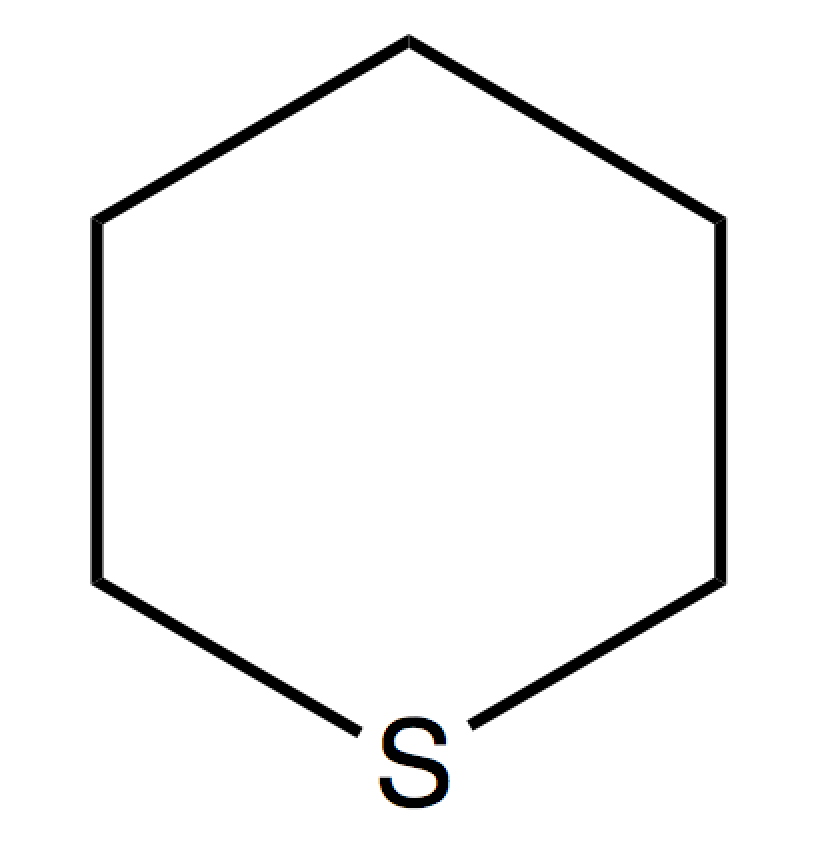
\includegraphics[scale=0.08]{image/sulfure-cycle} & Sulfures cycliques \\
			RSSR' & Disulfures \\
			 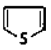
\includegraphics[scale=0.08]{image/thiophene} & Thiophène \\
			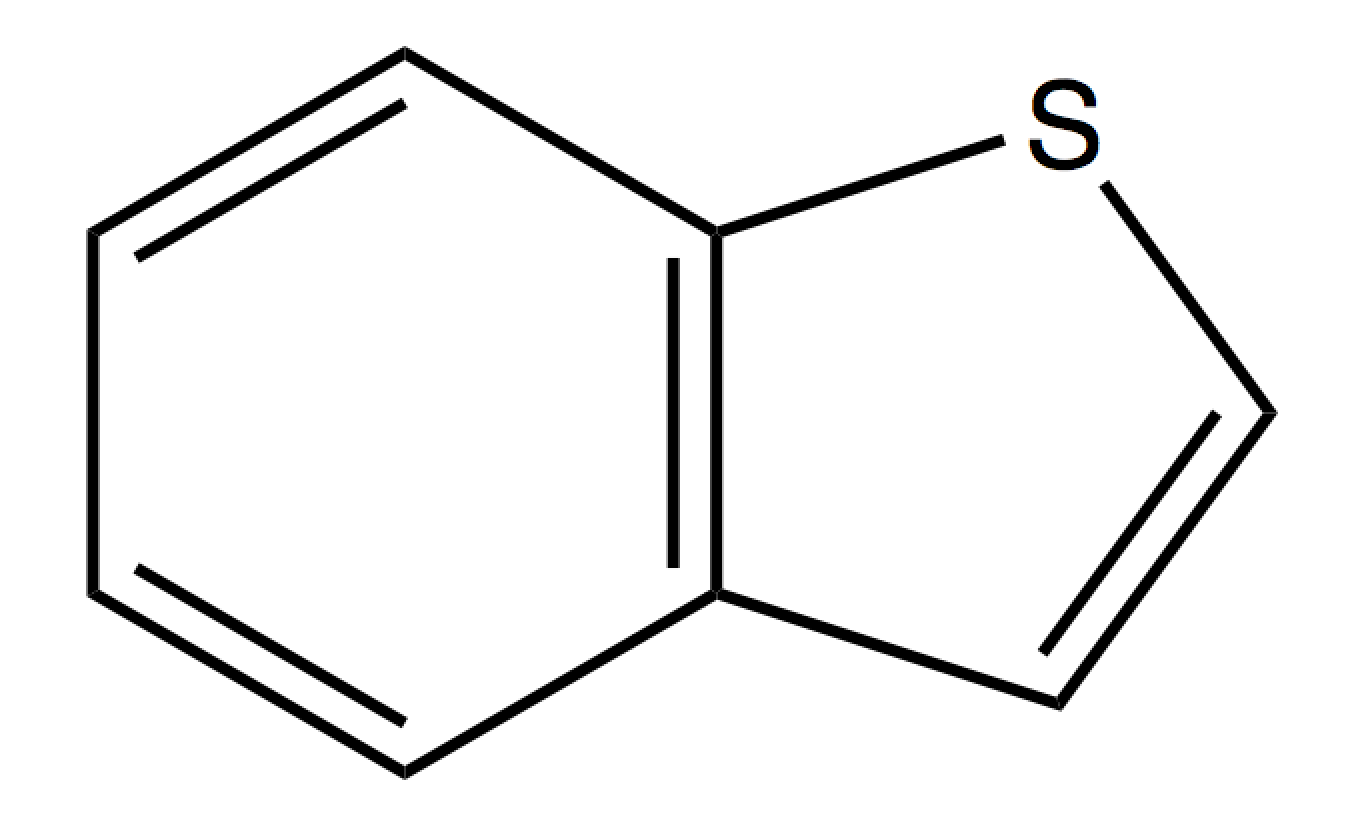
\includegraphics[scale=0.08]{image/benzothiophene} & Benzothiophène \\
			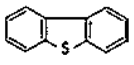
\includegraphics[scale=0.08]{image/dibenzothiophene} & Dibenzothiophène \\
			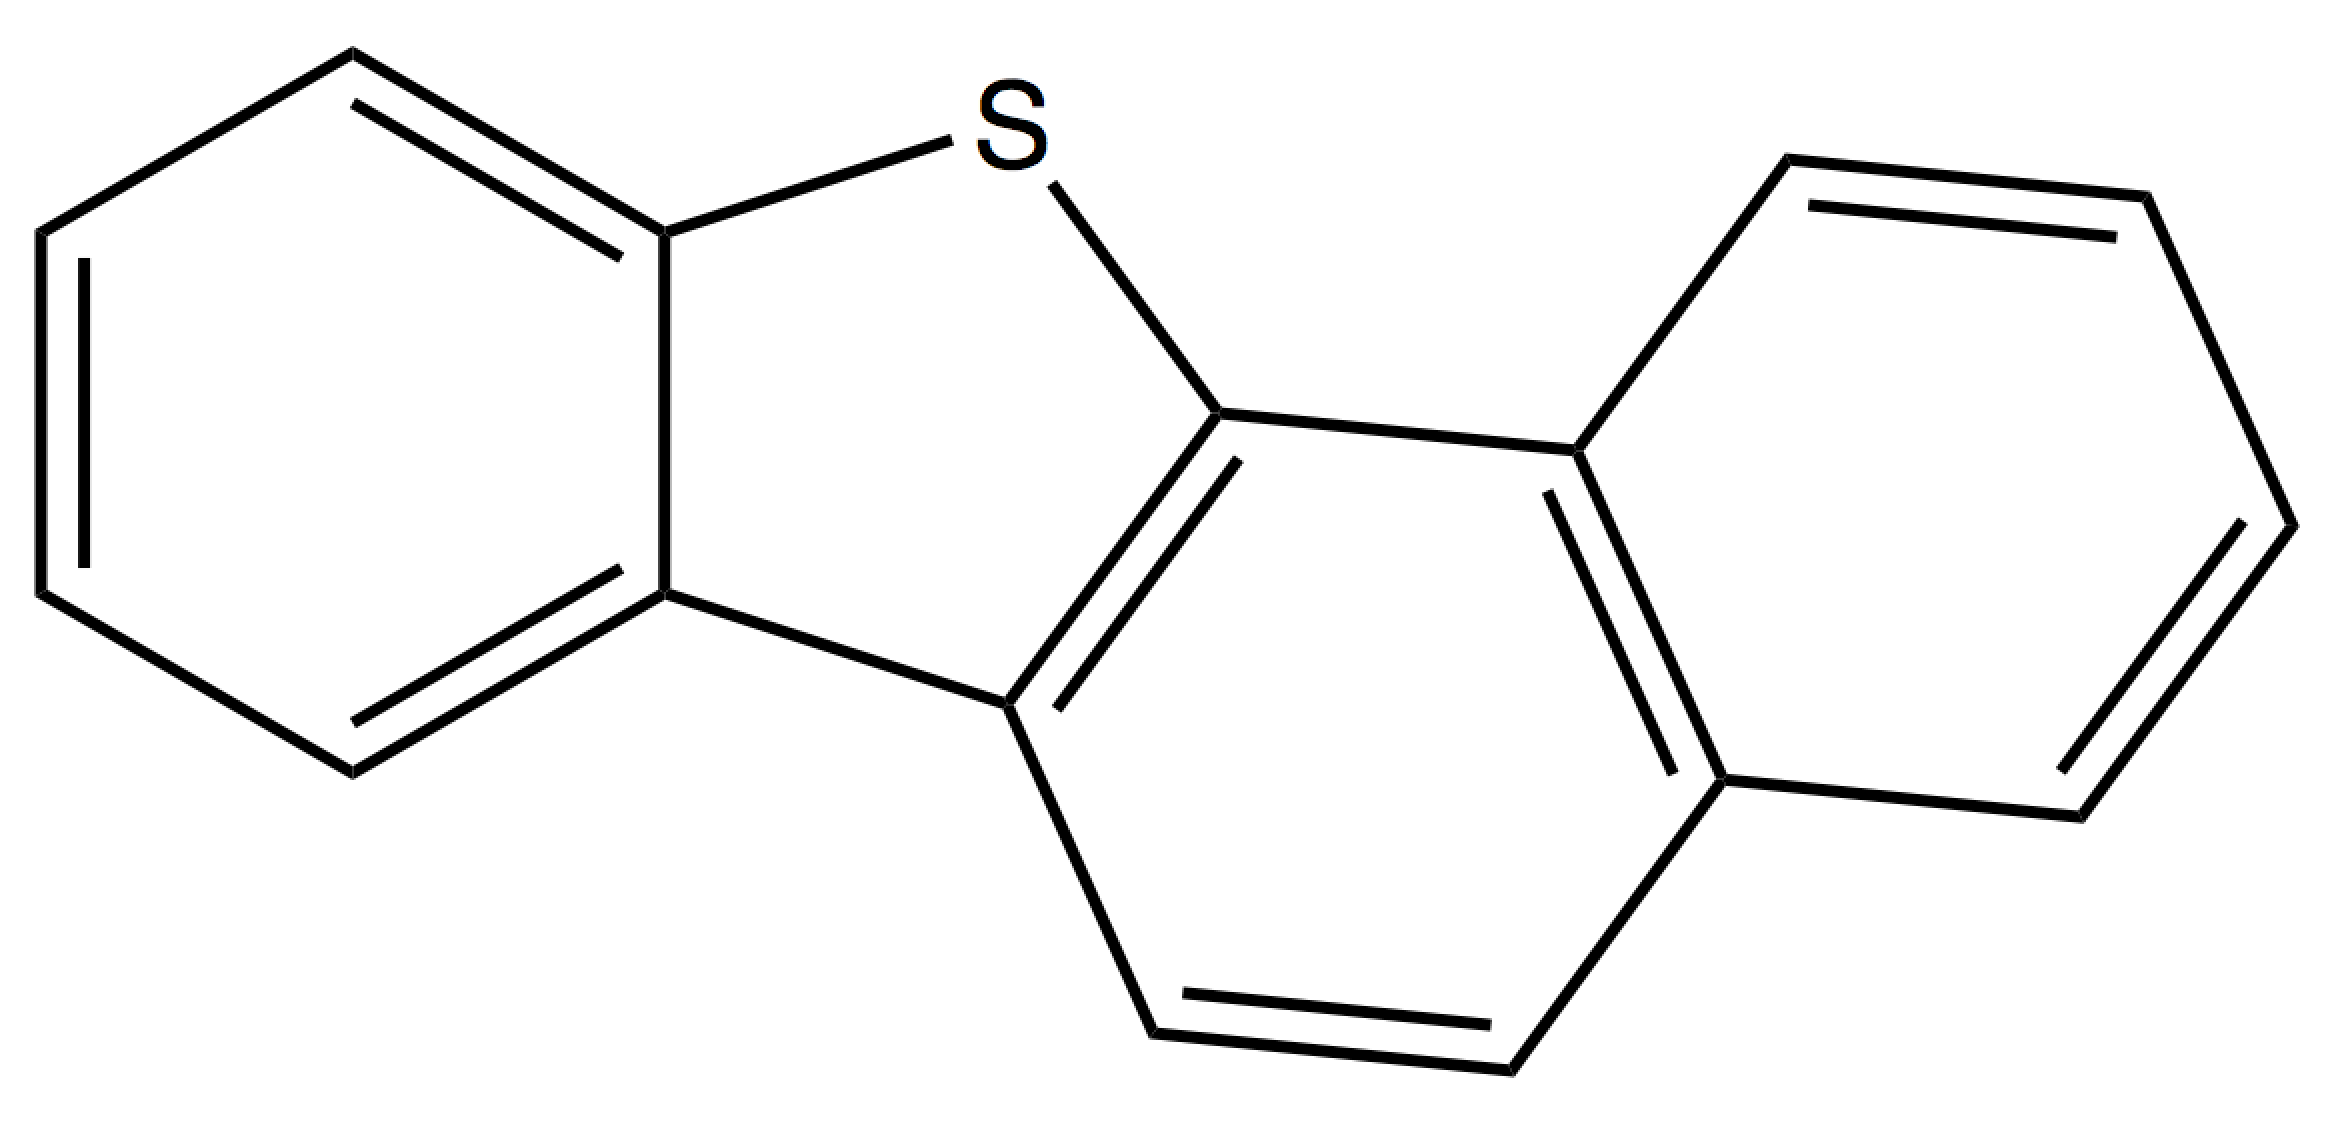
\includegraphics[scale=0.08]{image/naphto1} & Naphtobenzothiophènes \\
			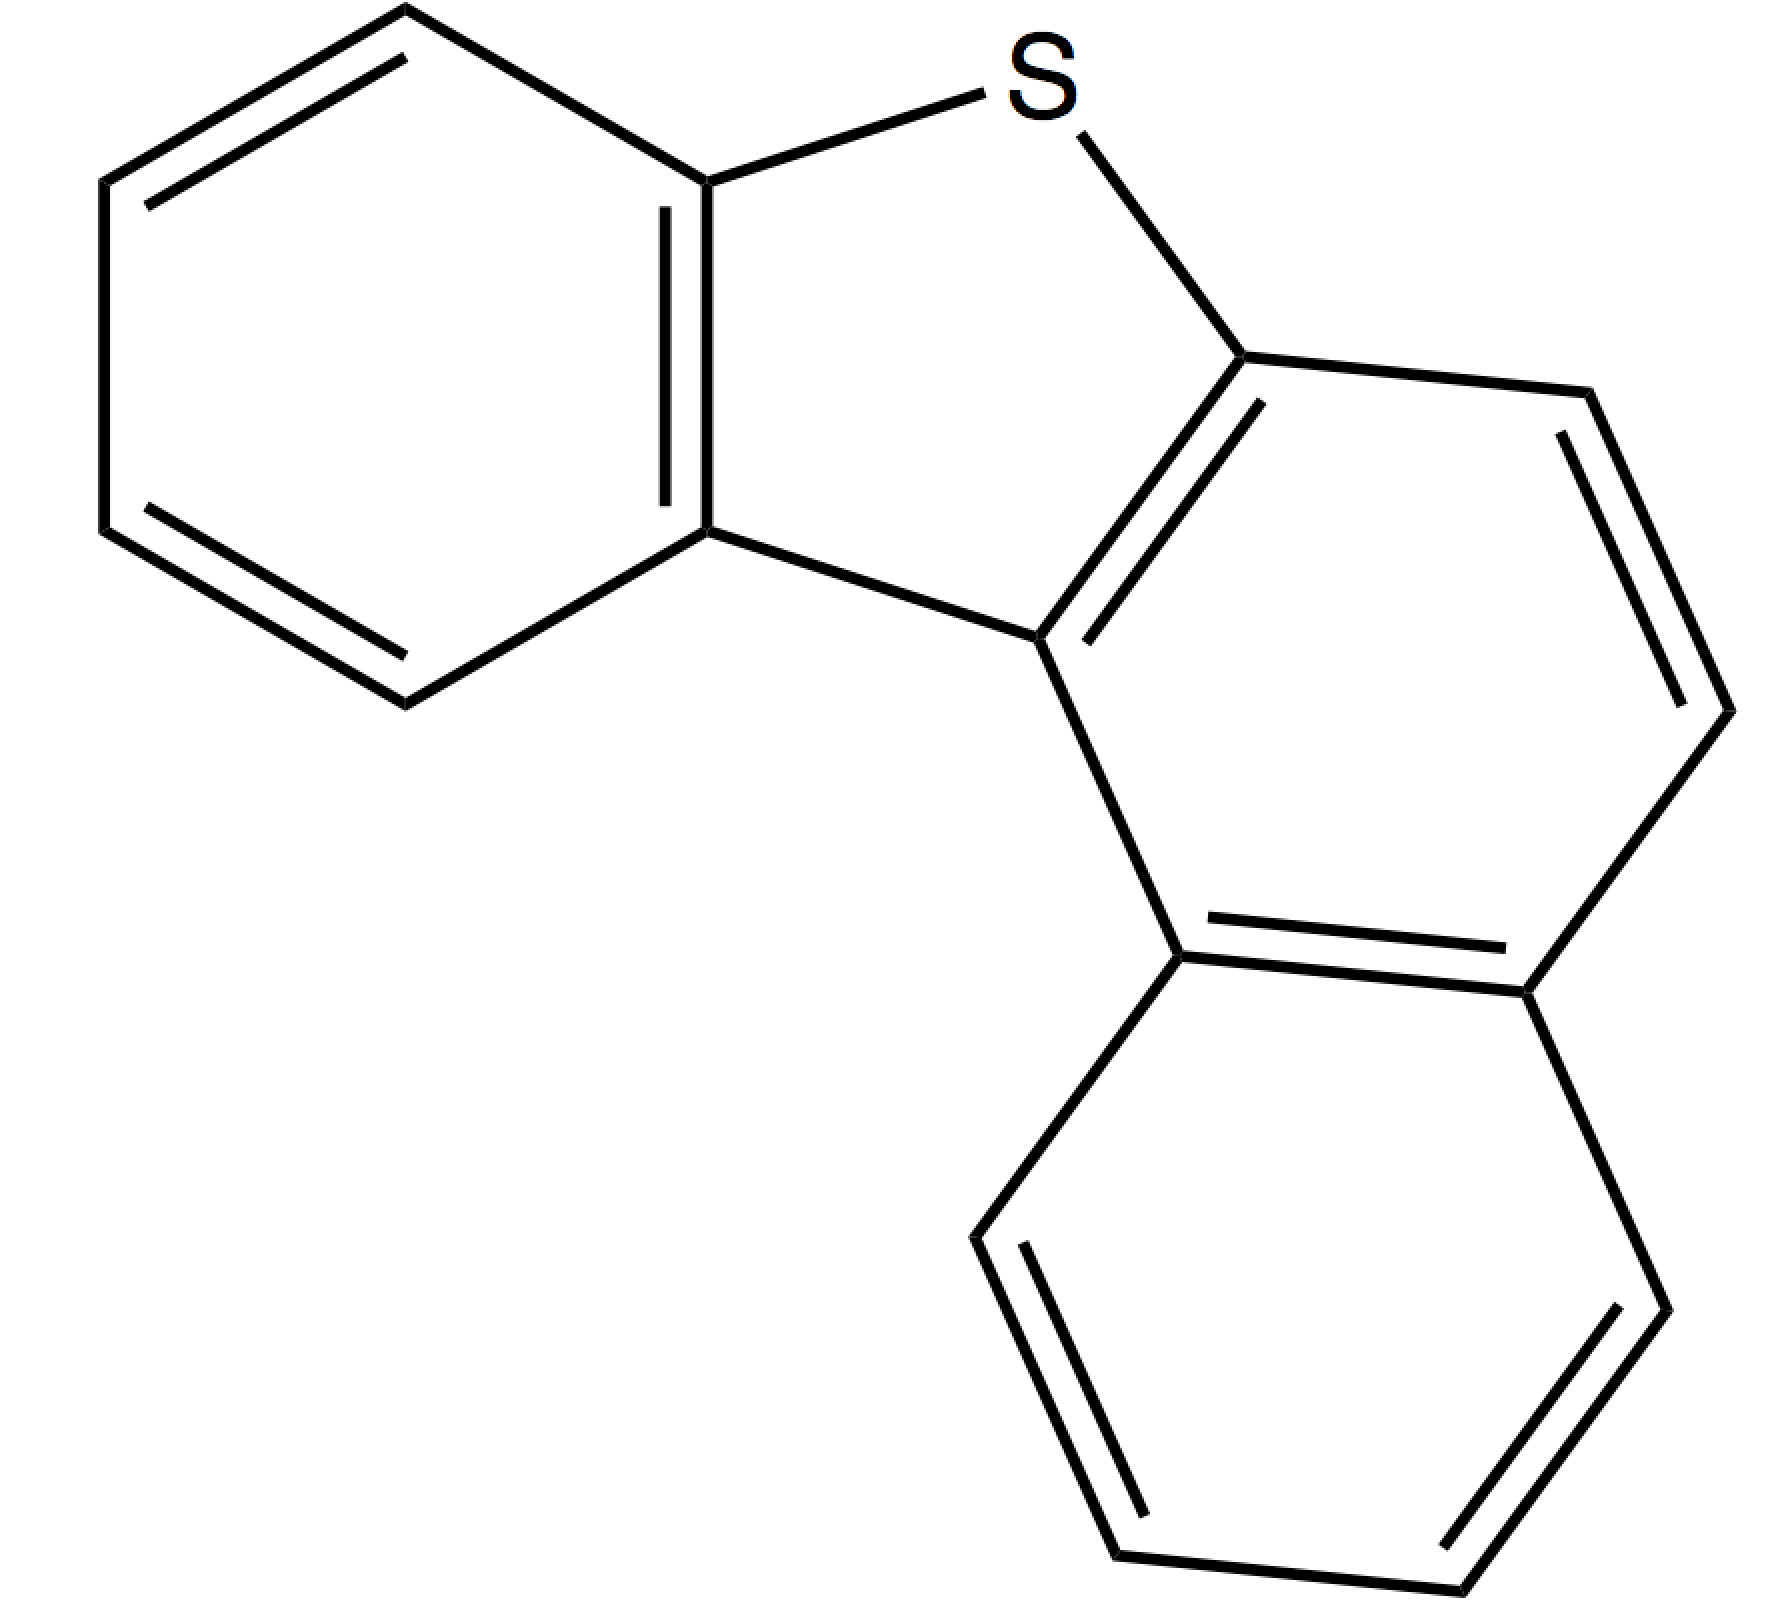
\includegraphics[scale=0.08]{image/naphto2} & \\
			\hline 
		\end{tabular}
	\end{center}
	\caption{Famille de composés soufrés caractérisés au sein du pétrole brut}
	\label{tab:soufre}
\end{table}


Thiols, sulfures, sulfoxydes et disulfides peuvent être classés plus précisément suivant leur nature cyclique ou acyclique, soit suivant l'organisation du squelette carboné (alkyle, aryle ou alkyl-aryle). Les dérivés thiophéniques, quant à eux, sont des structures polyaromatiques condensées autour d'un noyau thiophène (benzo, dibenzo, naphtobenzo-thiophènes, etc.). Au sein des fractions lourdes, la majorité des espèces soufrées sont des dérivés thiophéniques (cf. tableau \ref{tab:soufre-ex}), suivi par des dérivés sulfures (cycliques et acycliques). Enfin, des espèces de type sulfoxydes ont été mises en évidence, dans des proportions très variables, leur teneur variant entre 0.3\% et 10.3\% \cite{merdrignac2007physicochemical, speight2004petroleum}.

\begin{table}[h!]
	\begin{center}
		\begin{tabular}{rl}
			\hline
			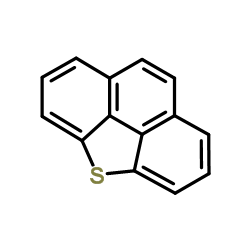
\includegraphics[scale=0.4]{image/phenanthro-thiophene} & Phénanthro-thiophènes \\
			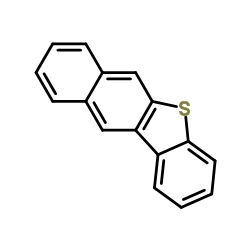
\includegraphics[scale=0.4]{image/benzo-naphto-thiophene} & Benzonaphto-thiophènes \\
			\hline 
		\end{tabular}
	\end{center}
	\caption{Exemples de dérivés thiophéniques courants identifiés au sein des fractions lourdes : phénanthro-thiophènes et benzonaphto-thiophènes}
	\label{tab:soufre-ex}
\end{table}


\paragraph{Azote}
En dépit des faibles proportions dans lesquelles il est présent, les dérivés de l'azote sont particulièrement étudiés, puisqu'à l'origine de la destruction des catalyseurs employés lors du craquage. Comme leurs analogues soufrés, les composés azotés se retrouvent en majeure partie au sein des fractions lourdes et des résidus de distillation du pétrole. \\
On distingue communément deux classes de composés azotés, à savoir les dérivés dits \og \textit{basiques} \fg, qui regroupent les homologues de la pyridine, et les dérivés dits \og \textit{neutres} \fg, qui rassemblent des systèmes de type pyrrole, indole et carbazole.  
En règle générale, environ un tiers des composés azotés sont des dérivés "basiques", la part restante revenant donc aux composés dits "neutres", bien que ces proportions puissent varier sensiblement en fonction des paramètres géochimiques de provenance du pétrole. \\
Comme indiqué dans le tableau \ref{tab:azote}, les structures "basiques" identifiées sont des analogues de la pyridine, tels que la quinoléine ou l'iso-quinoléine, comprenant entre deux et quatre cycles aromatiques condensés avec différents degrés d'alkylation ; des benzo- et dibenzoquinoléines, tétrahydroquinoléines, ainsi que des azapyrènes, ont par exemple pu être caractérisés, qui forment autant de systèmes à haut encombrement stérique. \\

\begin{table}[h!]
	\begin{center}
		\begin{tabular}{rl}
			\hline
			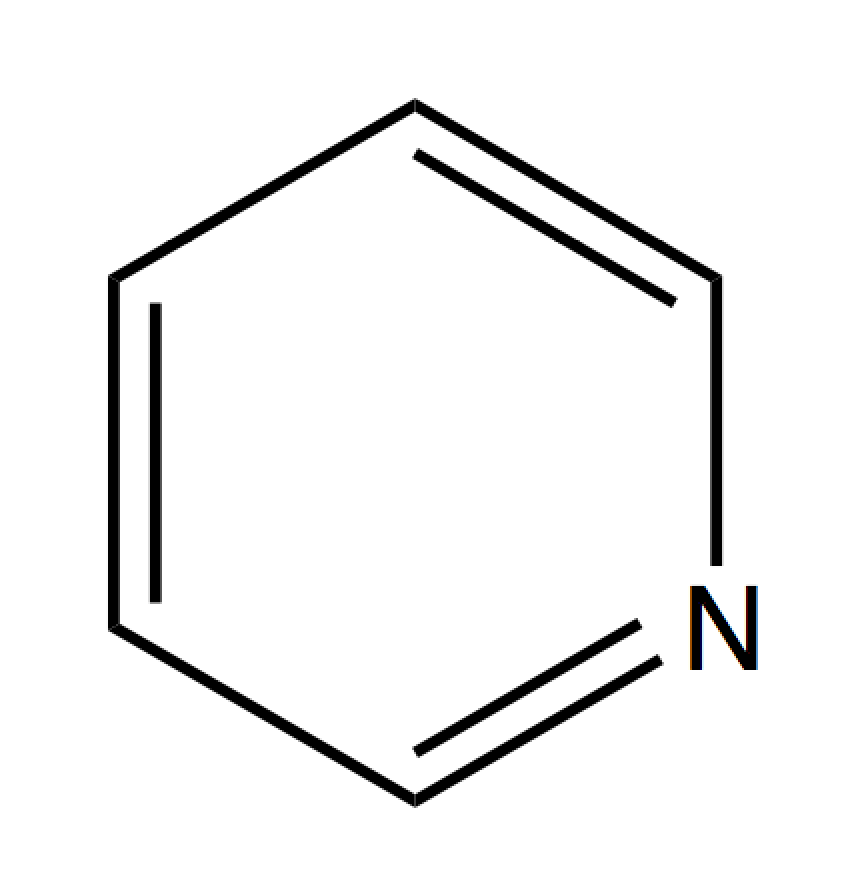
\includegraphics[scale=0.08]{image/pyridine} & Pyridine \\
			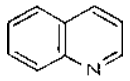
\includegraphics[scale=0.08]{image/quinoline} & Quinoline \\
			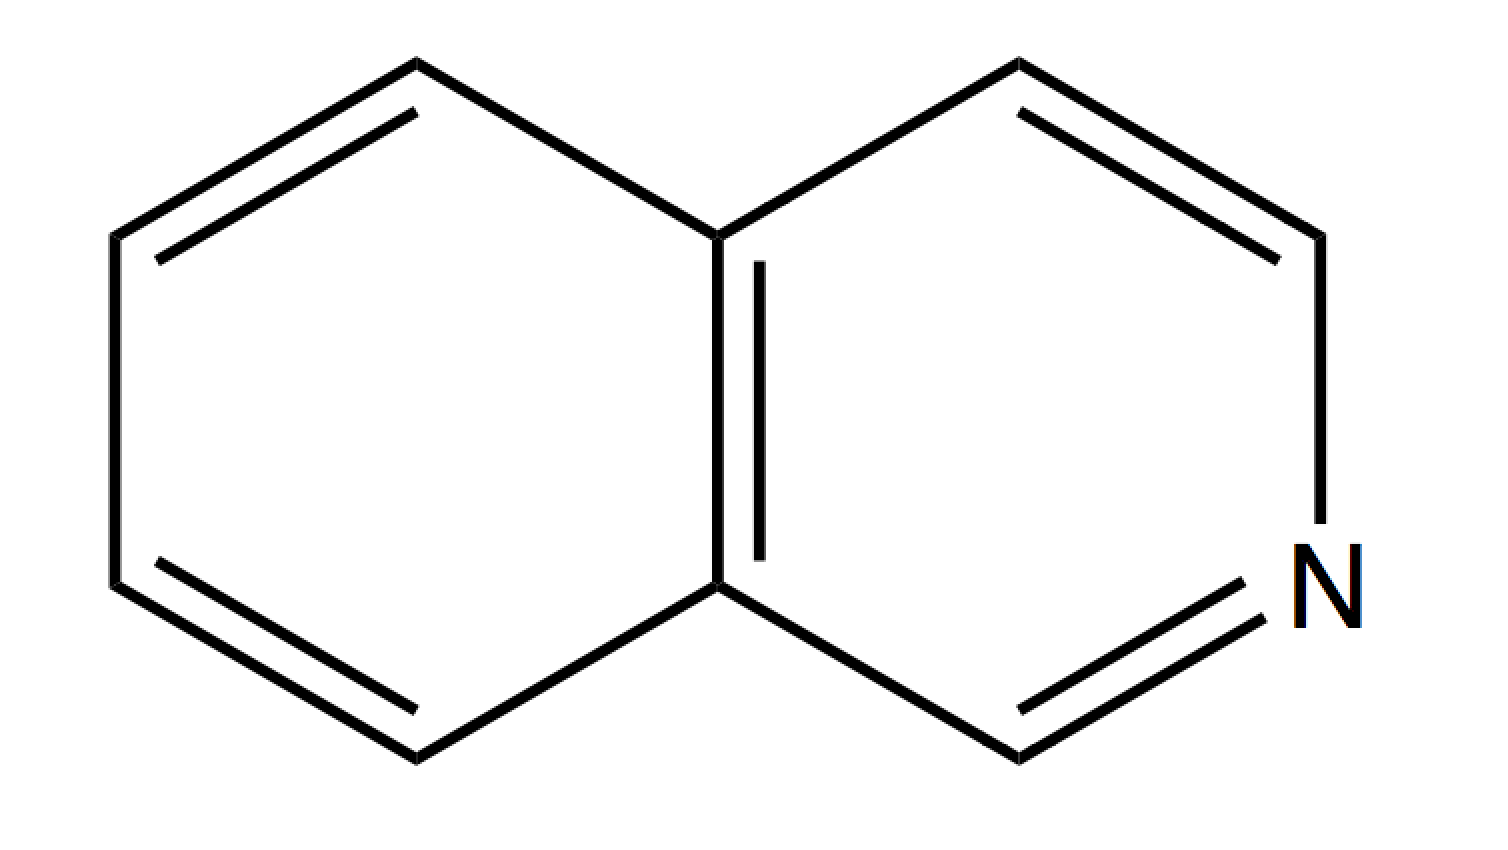
\includegraphics[scale=0.08]{image/isoquinoline} & Isoquinoline \\
			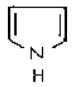
\includegraphics[scale=0.08]{image/pyrrole} & Pyrrole \\
			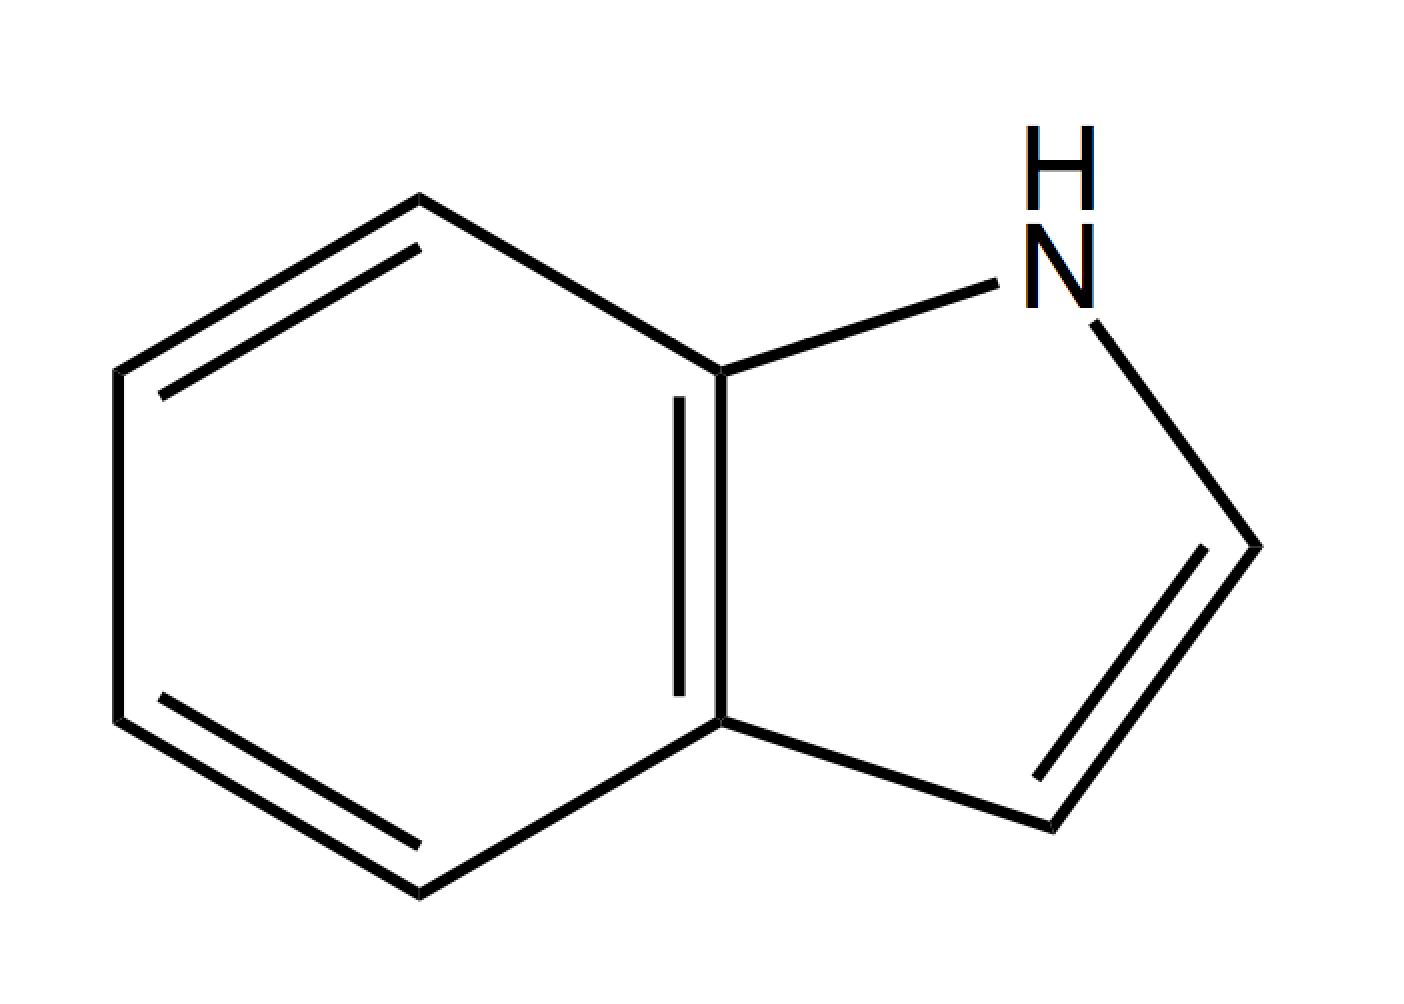
\includegraphics[scale=0.08]{image/indole} & Indole \\
			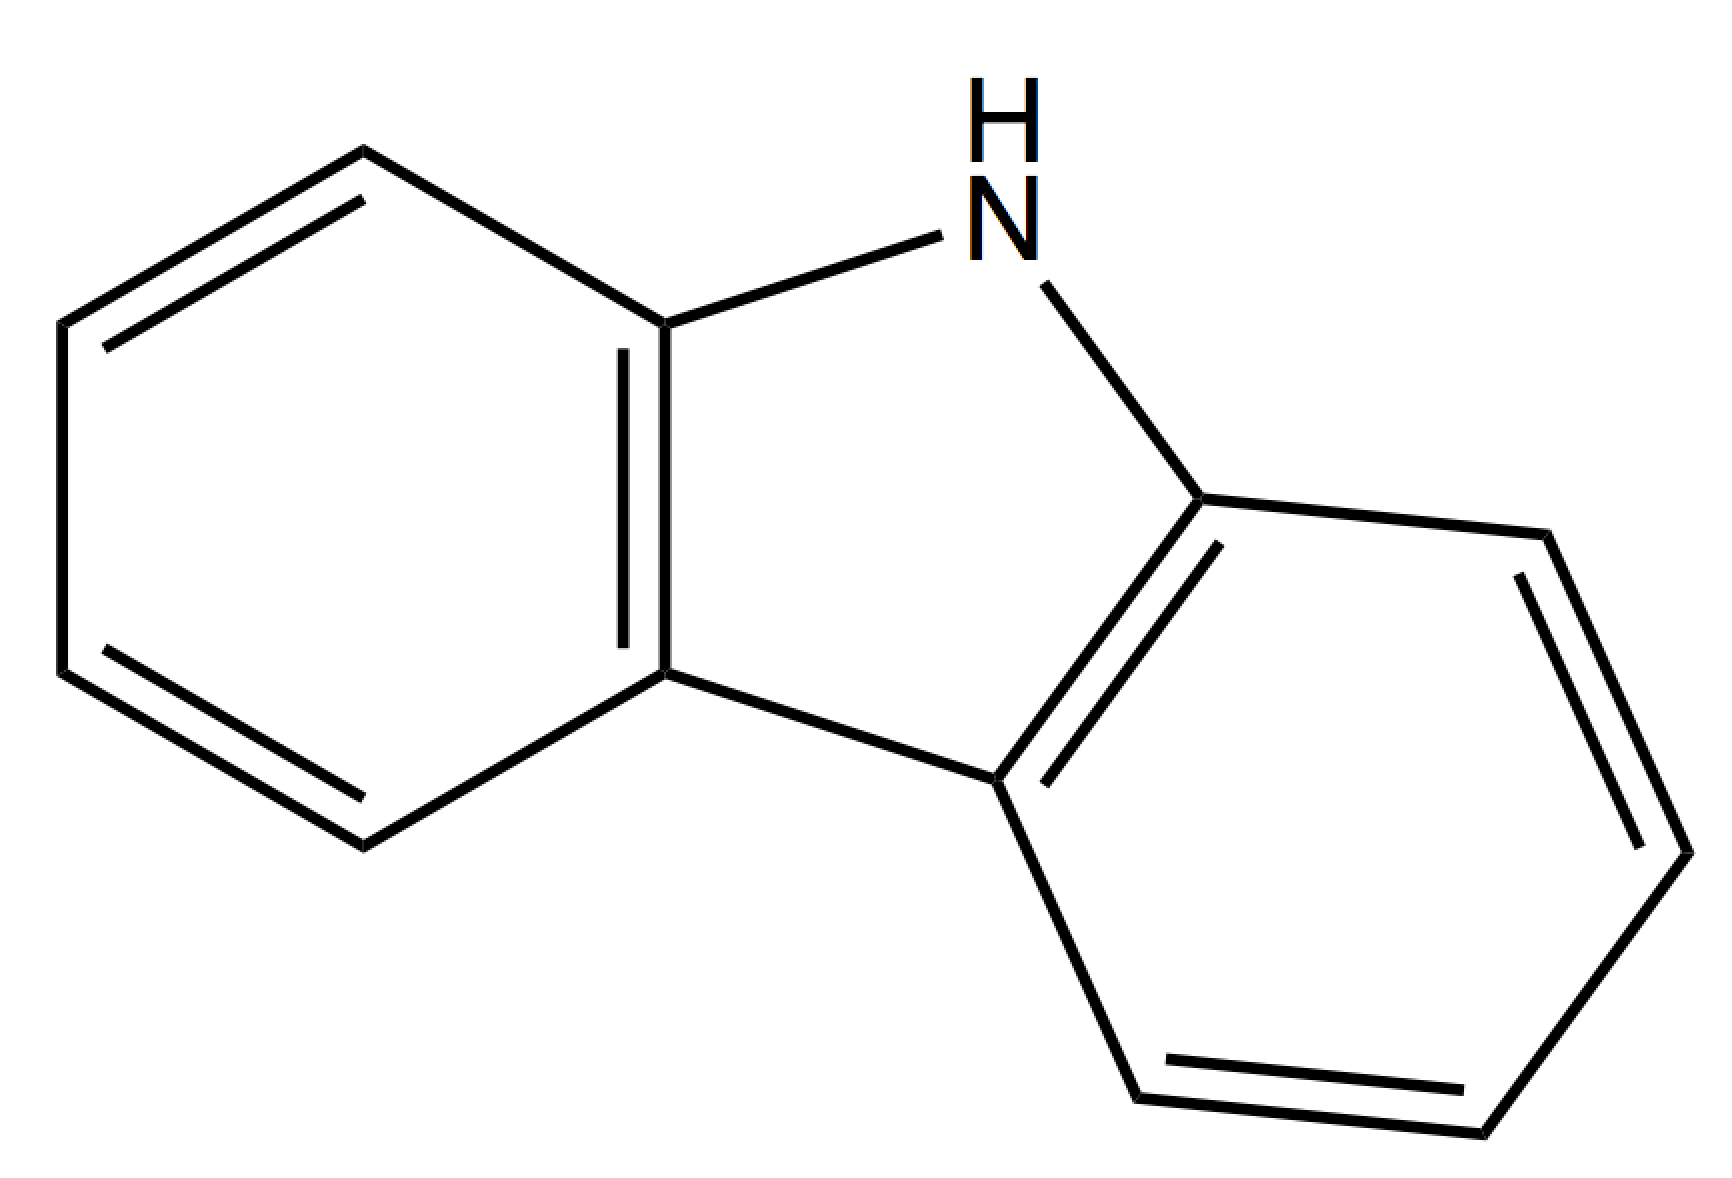
\includegraphics[scale=0.08]{image/carbazole} & Carbazole \\
			\hline 
		\end{tabular}
	\end{center}
	\caption{Famille de composés azotés caractérisés au sein du pétrole brut}
	\label{tab:azote}
\end{table}


Les structures "neutres", majoritaires, sont essentiellement représentées par les dérivés carbazolés (benzo-carbazoles, dibenzo-carbazole, etc.). C'est également au sein de cette classe de composés que l'on trouve les porphyrines qui, bien que présentes en proportions plus anecdotiques, possèdent une stabilité remarquable. La brique élémentaire de ces systèmes de grande taille est la molécule de pyrrole, et la plus simple des porphyrines est constituée par l'assemblage de quatre molécules de pyrrole [figure porphine !!!], reliées par des ponts méthylène =CH--. Le large système de résonance ainsi formé augmente considérablement la stabilité des structures ainsi formées. Par ailleurs, les porphyrines ont tendance à former des complexes métalliques avec les ions nickel et vanadium présents au sein du pétrole, par substitution des deux atomes d'hydrogène liés aux atomes d'azote de la structure porphyrinique. La proportion de ces structures au sein du pétrole dépend une nouvelle fois de l'origine géochimique de ce dernier, et un nombre croissant d'études s'intéresse à la part de métaux présents dans les huiles brutes. On estime aujourd'hui que ces complexes porphyrine-métaux représentent entre 0.6 et 3.3\% des fractions lourdes extraites\cite{merdrignac2007physicochemical, speight2004petroleum}.

\paragraph{Oxygène}
Au sein des fractions lourdes qui nous intéressent, la teneur en composés oxygénés varie entre 0.3 et 4.9\% \cite{speight2004petroleum}. Ces composés oxygénés figurent parmi les premières espèces caractérisées du pétrole. Les premiers travaux reportant la présence d'espèces acides au sein du pétrole remontent à 1874, et il faudra attendre quelques années de plus avant que celles-ci ne soient formellement identifiées comme étant des acides carboxyliques. Avec les dérivés du phénol, les acides carboxyliques représentent la majorité des espèces oxygénées constituant le pétrole, que l'on retrouve aussi bien dans les fractions lourdes qu'au sein de fractions plus légères. L'ensemble des études réalisées sur le sujet tend à établir que la structure de ces acides carboxyliques correspond à la structure de l'hydrocarbure prévalent. En d'autres termes, la structure de l'acide dépend du nombre d'atomes de carbone que compte le squelette carboné de l'hydrocarbure. Ainsi, lorsque l'acide comporte moins de huit atomes de carbone, ce qui correspond à un hydrocarbure de type paraffinique comme évoqué ci-avant, sa structure sera de type aliphatique. Suivant cette logique, des acides comportant un cycle commencent à apparaître à partir de six atomes de carbone et ces structures monocycliques prédominent jusqu'à quatorze atomes de carbone environ. \\
Une caractérisation plus fine des groupements carboxyles en présence révèle également la coexistence d'esters, de cétones, d'amides, d'anhydrides, d'éthers et de sulfoxydes. Néanmoins, à la différence des acides carboxyliques, plus aisés à caractériser puisque présent tant dans les fractions lourdes que dans les fractions légères, ces composés oxygénés se retrouvent majoritairement dans les fractions lourdes et leurs structures sont de fait plus complexes à identifier. Il est par ailleurs à noter que certains de ces composés sont supposés provenir de réactions entre les résidus de distillation et l'oxygène soufflé, qui intervient notamment dans les procédés de production de l'asphalte. De fait, il est difficile de conclure quant au fait que toutes ces espèces sont ou non des constituants du pétrole brut. 


\subsubsection{Débat autour du poids moléculaire des asphaltènes}

Un rapide passage en revue de la bibliographie des asphaltènes révèle tout le débat autour de leur poids moléculaire. En effet, la distribution, en termes de poids moléculaire, varie entre 400 et 1500 Da pour les fractions de faible poids moléculaire, et peut atteindre $10^{6}$ Da pour les fractions de haut poids moléculaire \cite{mullins2008contrasting}. Le phénomène d'agrégation des asphaltènes est une des raisons avancées pour justifier qu'à l'heure actuelle aucune méthode n'ait permis de déterminer avec précision le véritable poids moléculaire de ces espèces. De nombreux procédés ont été employés pour tenter de résoudre ce problème, mais ceux-ci conduisent à des résultats ambigüs, qu'il serait hasardeux de généraliser. À titre d'exemple, des mesures par osméométrie à tension de vapeur font apparaître des résultats fortement dépendants du type de solvant employé ; en présence d'un solvant apolaire tel que le toluène, les résultats apparaissent surestimés, au contraire de l'utilisation d'un solvant polaire tel que la pyridine ou le nitrobenzène. 
%S'agissant d'autres méthodes d'analyse, Groenzin et Mullins\cite{groenzin2000molecular} parviennent, par spectroscopie de fluorescence résolue en temps, à un poids moléculaire moyen de 750 Da environ, pour une distribution de 500 à 1000 Da, là où Pinkston et col.\cite{pinkston2009analysis} rapportent une distribution de 350 à 1050 Da pour une étude par spectrométrie de masse de résonance cyclotronique ionique à transformée de Fourier (FT-ICR). Ces derniers supposent l'existence de fragments de plus bas poids moléculaires, non détectés même à haute énergie électronique du fait de la stabilisation des intermédiaire obtenus par les chaînes alkyles des asphaltènes. 

%Merdrignac et col.\cite{merdrignac2006evolution} rapportent l'évolution du poids moléculaire des asphaltènes et comparer les changements causés par le procédé d'hydroconvertion. 


%\subsubsection{Une inconnue : la structure des asphaltènes}

\section{État des lieux des connaissances sur les systèmes asphalténiques}

La description de la structure des asphaltènes repose à l'heure actuelle sur deux modèles construits sur la base des résultats de diverses caractérisations expérimentales.  
Le premier modèle, baptisé modèle \og continental \fg, représente les asphaltènes comme de larges cœurs constitués de quatre à dix cycles aromatiques condensés, ramifiés par des chaînes alkyles courtes \cite{groenzin2000molecular} (cf. figure \ref{figZ1}). Ce modèle a été proposé par Zhao \textit{et al.} \cite{zhao2001molecular} après caractérisation des asphaltènes obtenus par fractionnement avec du pentane supercritique, puis remployé par Rogel et Carbognani \cite{rogel2003density} dans leur travail sur des asphaltènes stables et instables extraits de pétrole provenant du Vénézuela. 
Ce type de représentations est corrélé par des analyses en spectroscopie RMN, diffraction des rayons X et spectroscopie de fluorescence résolue en temps (TRDF). 



\begin{figure}[h!]
	\centering
	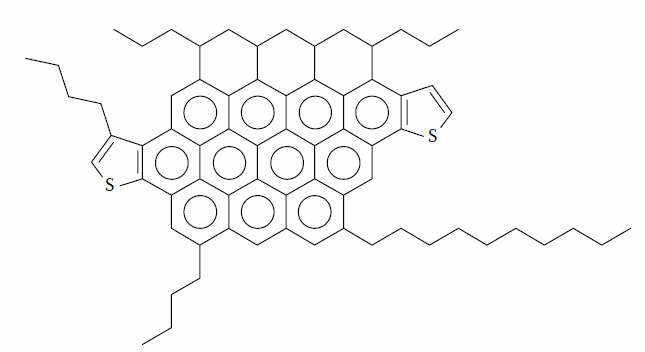
\includegraphics[height=5cm]{image/Zhao}
	\caption[Structure moyenne du modèle continental des asphaltènes]{Structure moyenne du modèle continental des asphaltènes (Zhao et col. \cite{zhao2001molecular})}
	\label{figZ1}
\end{figure}


Le modèle "archipel" présente quant à lui ces systèmes comme un ensemble de régions à caractère aromatique, constituées de deux à trois cycles condensés, reliées par des chaînes carbonées. Ce modèle s'appuie sur des analyses par pyrolyse, oxydation, dégradation thermique et dispersion angulaire neutronique, telles que rapportées par Gawrys \textit{et al.} \cite{gawrys2003role}. Sheremata \textit{et al.}\cite{sheremata2004quantitative} ont notamment employé ce modèle pour la description des asphaltènes, comme le présente la figure reproduite ci-après (figure \ref{fig2}). 

\begin{figure}[h!]
	\centering
	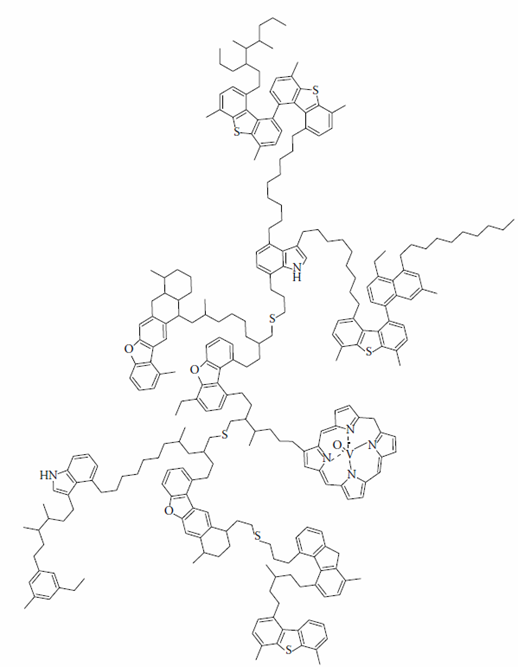
\includegraphics[height=8cm]{image/Sher}
	\caption[Molecule d'asphaltènes type archipel]{Représentation d'asphaltènes à l'aide du modèle archipel, proposé par Sheremata \textit{et al.}\cite{sheremata2004quantitative}}
	\label{fig2}
\end{figure}

Ces deux modèles, basés sur des structures moléculaires bien distinctes, conduisent néanmoins à des propriétés physico-chimiques différentes. La description des agrégats d'asphaltènes ainsi que leur solubilité dans le pétrole brut seront nettement impactées par l'emploi de l'une ou l'autre de ces représentations. Du fait de la planéité induite par la présence d'un grand nombre de cycles aromatiques condensés, la représentation d'un agrégat d'asphaltènes dans le cadre du modèle continental conduit à un empilement de plans. À l'inverse, les chaînes alkyles du modèle archipel confèrent une toute autre géométrie à ces systèmes : les asphaltènes peuvent se courber par le biais d'interactions intermoléculaires pour former des macro-agrégats globulaires susceptibles de piéger les molécules de solvant. \bigskip

Le paragraphe qui suit se veut résumer les nombreuses analyses expérimentales menées sur ces systèmes, analyses qui ont dans un premier temps permis l'émergence des deux modèles que nous venons d'évoquer, avant de travailler à les confirmer ou les infirmer. 

\subsection{Revue des données expérimentales}

\subsubsection{Analyses par spectroscopie RMN}

La spectroscopie de résonance magnétique nucléaire est couramment employée pour l'analyse structurale et la caractérisation de matériaux et de substances organiques. 
%Elle est fondée sur les propriétés magnétiques de certains noyaux atomiques.Les noyaux les plus étudiés, dans le cadre de la chimie organique sont l'hydrogène $^{1}H$ et le carbone $^{13}C$. 
Cette technique représente donc une méthode d'analyse de choix pour l'étude des asphaltènes et a, à ce titre, permis d'acquérir les premiers résultats visant à résoudre leur composition chimique. Dès 1982, les travaux de Murphy \textit{et al.} \cite{murphy1982determination} révèlent que la structure primaire des asphaltènes se compose de multiples cycles aromatiques condensés (l'indice de condensation relevé sur ces systèmes étant de 3 au moins) ainsi que d'une grande variété de chaînes aliphatiques, longues et ramifiées. Par la suite, les travaux de Yen \textit{et al.} en RMN $^{1}H$ ont donné une première idée de la proportion d'hydrocarbures saturés en regard de la fraction d'hydrocarbures aromatiques au sein de molécules d'asphaltènes  \cite{yen1984study}. Enfin, plus récemment, Durand \textit{et al.} ont employé les résultats de leurs analyses par RMN $^{13}C$ pour évaluer les indices de substitution et de condensation d'échantillons d'asphaltènes de différentes origines \cite{durand2010effect}. Leur étude tend à démontrer qu'au sein d'agrégats d'asphaltènes cohabitent les deux modèles structuraux évoqués ci-avant, à savoir le modèle continental et le modèle archipel. 


\subsubsection{Analyses par diffraction des rayons X}  

Une étude du caractère aromatique et des paramètres cristallins des asphaltènes, des résines et des gilsonites issus du pétrole a été présentée par Yen \textit{et al.} sur la base d'analyses en diffraction des rayons X \cite{yen1961investigation}. Leurs résultats, confortés par les travaux réalisés par Shirokoff \textit{et al.} sur quatre échantillons d'asphaltènes issus d'huiles brutes provenant d'Arabie Saoudite \cite{shirokoff1997characterization}, représentent les asphaltènes comme des feuillets de cycles aromatiques condensés portant des ramifications de natures naphténiques et aromatiques.
Toutefois, Altget et Boduszynky rappellent judicieusement dans leur étude \cite{altgeltcomposition} qu'il convient de prendre avec précaution les résultats provenant d'analyses de diffraction, lorsque les données géométriques fournies par l'analyse servent de base pour construire un modèle structural du système étudié. Leurs travaux semblent en outre indiquer que la détermination du caractère aromatique des asphaltènes est, par ce biais, inappropriée sinon arbitraire. 



\subsubsection{Analyses par spectroscopie de fluorescence résolue en temps} 

Cette méthode d'analyse a été employée à plusieurs reprises pour tenter d'élucider plus précisément la taille et la structure de molécules d'asphaltènes faiblement agrégées.  
Les premiers travaux en ce sens, réalisés par Groenzin et Mullins  \cite{groenzin1999asphaltene}, tendent à montrer que les molécules d'asphaltènes ne seraient constituées que d'un seul groupe chromophore. En effet, le faible poids moléculaire obtenu pour ces systèmes, comme la coloration des molécules, sont autant d'éléments recueillis incompatibles avec la représentation des asphaltènes sous forme de larges structures pseudo-polymériques constitués de deux ou trois cycles aromatiques reliés entre eux par de longues chaînes aliphatiques. En définitive, ces premières analyses par spectrométrie de fluorescence semblent conforter la représentation des asphaltènes par le modèle continental. \\
Par la suite, Souza \textit{et al.} ont rapporté l'agrégation persistante des asphaltènes à la faible concentration de 0.8 g/L, soit sous le seuil de concentration critique de nanoagrégation \cite{souza2009study}. Leurs travaux corroborent par ailleurs les résultats de Groenzin \textit{et al.}\cite{groenzin1999asphaltene} quant à la structure de type \og continental \fg{} des molécules d'asphaltènes, en cela qu'ils concluent à une structure primaire constituée d'un anneau polyaromatique de quatre cycles ou plus. 




\subsubsection{Analyses par spectroscopie infrarouge}

La caractérisation d'un système chimique en termes de composition passe nécessairement par des analyses en spectroscopie infrarouge, laquelle permet l'identification des groupements fonctionnels. Toutefois, dans le cadre de l'étude des fractions lourdes du pétrole, la diversité chimique et la taille des espèces présentes rendent complexe l'utilisation de la spectroscopie IR. C'est ce que soulignent Yuan \textit{et al.}, qui relèvent l'existence d'un faible nombre d'analyses employant l'infrarouge moyen pour la caractérisation physique et chimique des huiles lourdes \cite{hongfu2006determination}. 
Parmi les travaux notables, l'étude couplée en spectroscopies IR et UV-sisible menée par El-Bassoussi \textit{et al.}\cite{el2010characterization} sur deux échantillons d'asphaltènes provenant d'Egypte a permis de classifier les espèces présentes en mono, di et polyaromatiques. En accord avec les deux modèles de représentation des asphaltènes, les espèces prédominantes sont les espèces di ou polyaromatiques. En 2007, Rodrigues Coelho \textit{et al.} \cite{coelho2007characterization} démontrent l'existence d'une corrélation linéaire entre les intensités des bandes infrarouges symétriques et antisymétriques associées aux atomes d'hydrogène aromatiques de type arènes méthyl-substitués dans les régions 2900-3100 $cm^{-1}$ et 700-900 $cm^{-1}$. Enfin, Laxalde \textit{et al.} \cite{laxalde2014combining} rapportent une interprétation, toutefois ajustée sur les structures modèles des asphaltènes, en repérant les vibrations de stretching des liaisons C-H (hors du plan) et C=C.

\bigskip

\subsubsection{Conclusion : les asphaltènes, une coexistence de structures moléculaires ?}

La compilation de l'ensemble de ces résultats expérimentaux tend à suggérer que les deux modèles structuraux des asphaltènes peuvent coexister au sein des fractions lourdes. Cette idée est appuyée par les résultats d'Acevedo \textit{et al.} \cite{acevedo2004structural, gutierrez2001fractionation} qui ont montré que les asphaltènes pouvaient se diviser en deux fractions : une fraction insoluble dans le toluène, baptisée A1, qui serait rigide et plane, conformément au modèle continental, et une fraction soluble dans le toluène grace à de nombreuses interactions intermoléculaires, baptisée A2 et qui correspondrait au modèle archipel. Sur la base de ces éléments, Acevedo et son équipe ont mis en place une nouvelle représentation des agrégats d'asphaltènes. Le système colloïdal consisterait en une fraction d'asphaltènes A1, entourés par une couche d'asphaltènes A2, ces derniers aidant à la solubilisation de l'ensemble. \\
En définitive, une revue bibliographique des analyses expérimentales menées à ce jour sur les asphaltènes montre qu'aucun modèle structural définitif valide n'a encore émergé pour ce type de systèmes. De nombreux travaux cherchent encore à clarifier l'architecture moléculaire des asphaltènes, à deux échelles distinctes. En premier lieu, l'étude de la microstructure correspond à des systèmes de poids moléculaires variant entre 500 et 10 000 Da, soit à des nano-agrégats d'asphaltènes. En second lieu, les travaux sur la macrostructure de ces entités correspondent à l'étude d'assemblages de ces nano-agrégats d'asphaltènes et sont intimement liés au milieu. 



\subsection{La modélisation, outil indispensable dans l'élucidation des structures asphalténiques}

\subsubsection{Des nombreux intérêts de la modélisation des asphaltènes}

La chimie computationnelle a révolutionné notre façon d'appréhender la structure et la réactivité des molécules, de sorte que la simulation est désormais une des clés de voûte de l'avancée scientifique. \\
Comme nous l'avons souligné dans le paragraphe précédent, la nature et la complexité des asphaltènes rendent impossible leur caractérisation exhaustive par le seul biais de données expérimentales. Dans ce cadre, l'intérêt des simulations est incontestable et nombreux sont les travaux qui se sont déjà penchés sur la configuration moléculaire, les interactions intermoléculaires, la stabilité ou les phénomènes d'agrégation de ces systèmes.  
Concernant ce dernier point, la modélisation moléculaire a permis de justifier que l'agrégation des asphaltènes représentait la conformation la plus stable, sur la base d'une double approche structurale et thermodynamique révélant les interactions avec les résines, présentes au sein des fractions lourdes, et les solvants \cite{murgich1996molecular}. Selon ces travaux, l'interaction responsable de la formation comme de la stabilité des micelles formés d'asphaltènes et de résines serait la force d'attraction qui s'exerce entre les plans aromatiques. 
D'autres études théoriques se fondent sur les modèles structuraux proposés pour les asphaltènes. Les orbitales moléculaires de dimères d'asphaltènes, envisagés successivement par les modèles continental et archipel, ont été étudiés dans une approche semi-empirique ZINDO après optimisation des structures en DFT (théorie de la fonctionnelle de la densité). Du point de vue de la stabilité, la configuration continentale, représentée dans les simulations par des dimères empilés pour symboliser les plans d'asphaltènes propres à ce modèle, s'avère globalement plus stable que la configuration archipel \cite{alvarez2013island}. 


\subsubsection{Construction de la structure moléculaire des asphaltènes}

La construction d'un modèle moléculaire utilisable en simulation se fait sur la base des données expérimentales recueillies, suivant deux méthodes principales. \\
La première méthode repose sur une corrélation des résultats empiriques utilisés pour déduire des informations structurales. Dans le cas des asphaltènes, l'existence de nombreux cycles aromatiques et l'ensemble des données obtenues concernant la longueur des chaînes aliphatiques ont permis à Takanohashi \textit{et al.} d'étudier trois structures distinctes d'asphaltènes générées par la méthode de Sato par le biais de simulation en dynamique moléculaire \cite{takanohashi2004structural}. \\
La seconde méthode consiste à identifier des caractéristiques structurales propres au système, ainsi que sa composition moléculaire, en suivant un processus stochastique. Le modèle structural se construit alors par addition des données expérimentales et/ou par recoupement de ces résultats avec une base de données existantes. Cette méthode a été poursuivie aussi bien par Elyashberg \textit{et al.} \cite{elyashberg2008computer}, qui ont développé un algorithme permettant la construction d'une structure sur la base de données RMN, que par Todeschini \textit{et al.} \cite{todeschini1995weighted} qui ont quant à eux employé des propriétés physiques telles que l'hydrophobie, le point de fusion et le point d'ébullition. 
La construction d'un modèle moléculaire des asphaltènes peut en dernier lieu se faire initialement de façon plus intuitive, les informations expérimentales servant ensuite à optimiser le modèle de départ \cite{faulon1996stochastic}, \cite{al2012systematic}, \cite{de2012monte}. 





%\newgeometry{textwidth=16cm}
\chapter[Rappels théoriques : DFT]{Rappels théoriques : Méthodes de la fonctionnelle de la densité (DFT)}
\minitoc
\restoregeometry

\newpage

\section*{Introduction}
\markright{INTRODUCTION}{}

La chimie théorique est une science relativement récente, puisque ce n'est qu'en 1933 que le physicien autrichien Erwin Schr\"{o}dinger  a reçu le prix \textsc{Nobel} de physique, en commun avec Paul \textsc{Dirac}, pour ses travaux représentant, depuis, les fondements de la chimie quantique. En effet, l'équation de Schr\"{o}dinger nous prouve que la connaissance de la fonction d'onde du système donne accès, explicitement ou non, à toutes les valeurs caractéristiques du système chimique étudié. Dans l'article \textit{La situation actuelle en mécanique quantique}~\cite{schrodinger1992situation} paru en 1935, la métaphore du  \og chat de Schr\"{o}dinger \fg{} a largement contribué à la vulgarisation de cette science auprès du public scientifique. En effet, il y symbolise, à l'aide d'un exemple macroscopique régit par les lois de la physique classique, la philosophie de la mécanique quantique dévolue à l'étude des systèmes microscopiques. Le plus grand défi à relever ici était de faire comprendre qu'une \og mesure quantique \fg{} est une combinaison linéaire d'une somme d'états de probabilités non-nulles et non une valeur unique. L'expérience fictive consiste à placer un chat dans une boîte contenant un flacon de poison ainsi qu'une source radioactive. Lorsqu'un compteur Geiger détecte un certain seuil de radiation, un mécanisme vient briser le flacon et libère ainsi des vapeurs mortelles. Dans un raisonnement quantique, le chat est donc à la fois vivant \underline{et} mort dans la boîte tant qu'elle reste close, avec une probabilité de vie de plus en plus faible au cours du temps.\\

En pratique, le nombre considérable de calculs à réaliser dans le cadre de la chimie théorique lie intrinsèquement cette science au développement de l'informatique, tout aussi récent. Il s'agit même de l'une des plus grandes limites encore rencontrée de nos jours. Même si la loi de \textsc{Moore}~\cite{moore1965electronics}~\footnote{La loi de \textsc{Moore} (1965), renommée première loi de \textsc{Moore} compte-tenu de l'ajustement ultérieur, énonce que la complexité des semi-conducteurs (et donc de la puissance de calcul) suit une loi exponentielle au cours du temps.}, empirique de son état, a commencé à perdre en véracité dès lors que la fréquence des processeurs (CPU) engendrait une déperdition de chaleur trop importante et commercialement non-maîtrisable ($\gtrsim$ 5 Ghz), l'apparition des processeurs multic\oe urs s'est vu être la solution la plus efficace. Après l'adaptation nécessaire des codes séquentiels en version parallèle, la démocratisation relative des clusters de calcul~\footnote{Un cluster de calcul, ou grappe de serveurs, est un ensemble de serveurs esclaves, les n\oe uds, contrôlés par un ou plusieurs serveurs maîtres, le(s) frontal(aux). Ce groupe de serveurs indépendants, fonctionnant comme un seul et même système, permet d'optimiser les ressources (processeur, mémoire vive, stockage\dots{}) et une meilleure répartition des tâches sur les différents n\oe uds.} permet à l'heure actuel le développement de codes hautement parallélisés (> 1000 processeurs). Ceci permet alors de faire moins d'approximations théoriques et donc de tendre vers des valeurs de plus en plus exactes, tout en gardant des temps de calcul raisonnables. Un engouement pour les clusters de cartes graphiques (GPU) est aussi à noter dans les domaines scientifiques où, tel que la dynamique moléculaire, les calculs sont extrêment fragmentables et peu interdépendants.\\

Dans ce chapitre, nous rappellerons dans un premier temps les fondements de la théorie de la fonctionnelle de la densité, notée DFT, par le biais de l'évolution des différents modèles qui ont été proposés. Nous verrons ensuite comment les théorèmes de \textsc{Hohenberg} et \textsc{Kohn} prouvent que la seule connaissance de la densité électronique permet de résoudre l'équation de Schr\"{o}dinger dans le cadre de la DFT. La fonctionnelle universelle $F_{HK}[\rho]$, qui permettrait une résolution exacte du problème, restant inconnue, nous aborderons dans une troisième partie l'approche KS qui contourne ce problème et légitime certaines approximations. Ces dernières donnant naissance à différents types de fonctionnelle, elles seront succintement présentées dans la pénultième partie de ce chapitre. Finalement, le développement de la méthode de calcul utilisée dans ce travail de thèse, sera présentée étape par étape en fin de chapitre. 

\newpage

\section{Les fondements de la DFT}

Contrairement aux méthodes HARTREE-FOCK, noté HF, et \textit{a fortiori} post-HF qui décrivent le système électronique par une fonction d'onde $\Psi_{(\vec{r})}$, la théorie de la fonctionnelle de la densité le décrit par la densité électronique, notée $\rho_{(\vec{r})}$, qui est liée à la fonction d'onde $\Psi_{(\vec{r})}$ par la relation suivante~:

\begin{align}
\rho_{(\vec{r})} &= \int \Psi_{(\vec{r})}^{*} \Psi_{(\vec{r})} \\
&= \int |\Psi_{(\vec{r})}^{2}| \notag
\end{align}

\begin{flushleft}
\begin{tabular}{@{}lrp{10cm}}
avec & $\vec{r}$ : & ensemble des coordonnées électroniques. 
\end{tabular}
\end{flushleft}


L'énergie de l'état fondamental est ainsi une fonctionnelle de la densité électronique, c'est-à-dire que $E_{0} = E_{(\rho)}$.

\subsection{Modèle de \textsc{Thomas-Fermi}}

Le terme d'énergie cinétique a été exprimé comme une fonctionnelle de la densité pour la première fois en 1927 par \textsc{Thomas} et \textsc{Fermi}~:

\begin{equation}
\hat{T}_{TF}[\rho] = \frac{3}{10} (3\pi)^{2/3} \int \rho_{(\vec{r})}^{5/3} .d\vec{r}
\label{ener_cin_thom_ferm}
\end{equation}

Celle fonctionnelle est alors combinée aux expressions classiques des interactions électrons-noyaux et électrons-électrons, exprimées elles aussi en fonction de la densité électronique :

\begin{equation}
E_{TH}[\rho] = T_{TH}[\rho] + V_{Ne}[\rho] + V_{ee}[\rho]
\end{equation}

\subsection{Modèle de \textsc{Thomas-Fermi-Dirac}}

Le terme d'échange, résultant du principe d'exclusion de \textsc{Pauli}, a ensuite été ajouté par Dirac en 1930 afin d'affiner le modèle :

\begin{align}
K[\rho] = E_{x}[\rho] &= \int \rho_{\vec{r}} \epsilon_{x}[\rho] .d\vec{r} \\
&= -\frac{3}{4} \left(\frac{3}{\pi}\right)^{1/3} \int \rho_{(\vec{r})}^{4/3} .d\vec{r} \notag
\end{align}

\begin{flushleft}
\begin{tabular}{@{}lrp{10cm}}
avec & $\epsilon_{X}[\rho]$ : & énergie d'échange par électron. 
\end{tabular}
\end{flushleft}

Le modèle de \textsc{Thomas-Fermi-Dirac} est défini par la combinaison de cette expression avec l'équation~\ref{ener_cin_thom_ferm} et le potentiel d'interaction électrons-noyaux $V_{Ne}[\rho]$. Notons que la corrélation électronique n'est toujours pas prise en compte dans ce modèle.

\subsection{Modèle de \textsc{Slater}}

Partant d'une approche basée sur la méthode HF, \textsc{Slater} proposa en 1951 de substituer le terme d'énergie d'échange par une fonctionnelle de la densité issue de l'énergie d'échange de Dirac. Ce terme d'échange dans le formalisme HF peut alors être généralisé en introduisant le paramètre $\alpha$ :

\begin{equation}
E_{x}[\rho] = - \frac{9\alpha}{8} \left(\frac{3}{\pi}\right)^{1/3} \int \rho_{(\vec{r})}^{4/3} .d\vec{r}
\end{equation}

Des analyses empiriques basées sur différents types de systèmes chimiques ont conduit à une valeur de $3/4$ pour $\alpha$, offrant une meilleure précision que la valeur originelle de l'expression de Dirac ($2/3$).

\section{Les théorèmes de \textsc{Hohenberg} et \textsc{Kohn}}

Tous ces modèles, qui constituent les fondements de la DFT, ne démontrent pas formellement que seul la connaisance de la densité est importante pour atteindre la valeur de l'énergie totale d'un système. C'est ainsi que \textsc{Hohenberg} et \textsc{Kohn} eurent l'idée en 1965 de démontrer, par le biais de deux théorèmes, que l'équation de Schr\"{o}dinger pouvait être résolue de façon exacte, dans le cadre de l'approximation de \textsc{Born-Oppenheimer} uniquement grâce à la densité électronique.

\subsection{Premier théorème : preuve d'existence}

Ce premier théorème énonce que l'ensemble des propriétés du système, notamment l'énérgie, peuvent être calculées à partir de la seule densité électronique de l'état fondamental. Elles peuvent donc être décrites comme une fonctionnelle de la densité électronique, et l'énergie totale s'écrit alors :

\begin{equation}
E[\rho] = F_{HK}[\rho] + \int \rho_{(\vec{r})} \nu_{ext} .d\vec{r}
\label{Hohen_Kohn}
\end{equation}
\noindent où :
\begin{align}
F_{HK}[\rho] &= T_{e}[\rho] + V_{ee}[\rho] \\
\nu_{ext} &= V_{Ne}[\rho] \notag
\end{align}

Notons que la fonctionnelle universelle $F_{HK}[\rho]$, qui regroupe les termes d'énergie cinétique des électrons et celui d'énergie potentielle d'interaction électron-électron, n'est pas liée au potentiel externe $\nu_{ext}$. L'énergie de l'état fondamental est \textit{a priori} accessible de manière exacte car cette fonctionnelle ne repose sur aucune approximation.

\subsection{Second théorème : théorème variationnel}

Basé sur l'équation~\ref{Hohen_Kohn}, \textsc{Hohenberg} et \textsc{Kohn} ont ensuite construit un principe variationnel pour déterminer la densité électronique de l'état fondamental :

\begin{equation}
E[\rho] \geq E[\rho_{0}]
\end{equation}

\begin{flushleft}
\begin{tabular}{@{}lrp{10cm}}
avec & $\rho_{0}$ : & densité électronique de l'état fondamental, \\
& $\rho$ : & densité électronique quelconque.
\end{tabular}
\end{flushleft}

Dans cette équation, à une densité d'essai $\rho$ correspond une seule énergie potentielle $\int \rho_{(\vec{r})} \nu_{ext} .d\vec{r}$ et une seule fonction d'onde $\Psi_{\rho}$. La méthode de double minimisation, \textit{i.e.} sous contrainte de \textsc{Levy}, permet de différencier la fonction d'onde $\Psi_{\rho_{0}}$, correspondant à l'état fondamental, parmi le jeu infini des fonctions d'ondes $\Psi_{\rho}$ donnant la même densité. Ainsi, nous pouvons déterminer, parmi toutes les densités, celle qui minimisera l'énergie par la relation suivante :

\begin{equation}
E[\rho_{0}] = \min\limits_{\rho}\, (\min\limits_{\Psi\rightarrow\rho}\, (F[\rho] + \int \rho_{\vec{r}} \nu_{\vec{r}}\, .d\vec{r}\, ))
\end{equation}

Si les théorèmes de \textsc{Hohenberg} et \textsc{Kohn} démontrent une correspondance unique entre une densité $\rho_{\vec{r}}$ et la fonction d'onde $\Psi$ du système, la fonctionnelle universelle $F_{HK}[\rho]$ reste cependant inconnue.

\section{Approche Kohn-Sham}\label{Kohn-Sham}

Afin de contourner ce problème, \textsc{Kohn} et \textsc{Sham} substituèrent au Hamiltonien réel, décrivant un système de $n$ particules en interaction, un Hamiltonien de référence décrivant un système de $n$ particules sans interaction mais ayant la même densité que le système réel. Le problème est ainsi réduit à la résolution de $n$ équations monoélectronique couplées, analogues aux équations de HF. L'opérateur monoélectronique de Kohn-Sham $\hat{K}_{KS}$ s'exprime ainsi :

\begin{equation}
\hat{H}_{KS} = -\frac{1}{2} \nabla^{2} + \nu_{H}[\rho] + \nu_{xc}[\rho] + \nu_{ext}[\rho]
\end{equation}

\noindent où :
\begin{align}
\nu_{H}[\rho] &= \int \frac{\rho_{(\vec{r})} - \rho_{(\vec{r}')}}{|\vec{r} - \vec{r}'|} .d\vec{r}' \\
\nu_{xc}[\rho] &= \frac{\partial E_{xc}[\rho_{(\vec{r})}]}{\partial\rho_{(\vec{r})}}
\end{align}

\noindent $\nu_{H}[\rho]$ et $\nu_{xc}[\rho]$ étant respectivement le potentiel de \textsc{Hartree} et le potentiel d'échange et de corrélation, dans lequel $E_{xc}[\rho_{(\vec{r})}]$ est l'énergie d'échange et de corrélation.

En définissant un potentiel fictif $\nu_{eff(\vec{r})}$ pouvant être appliqué à des systèmes sans interaction de densité $\rho$ :

\begin{equation}
\nu_{eff(\vec{r})} = \nu_{H}[\rho] + \nu_{xc}[\rho] + \nu_{ext}[\rho]
\end{equation}

\noindent nous introduisons alors un jeu d'orbitales $\psi_{(\vec{r})}$, appelées orbitales de \textsc{Kohn-Sham}, et nous obtenons un jeu d'équations aux valeurs propres :

\begin{equation}
\hat{H}_{KS} \psi_{i(\vec{r})} = \epsilon_{i} \psi_{i(\vec{r})}
\end{equation}

Comme dans le cas de la méthode HF, l'énergie du système peut être minimisée en résolvant ce jeu d'équations de façon auto-cohérente grâce à l'utilisation des orbitales de \textsc{Kohn-Sham}. L'énergie du système est alors donnée par :

\begin{equation}
E_{KS}^{tot}[\rho] = T_{s}[\rho] + J[\rho] + E_{xc}[\rho] + \int V_{ext(\vec{r})}\rho_{(\vec{r})} .d\vec{r}
\end{equation}

\begin{flushleft}
\begin{tabular}{@{}lrp{10cm}}
avec & $T_{s}[\rho]$ : & énergie cinétique des électrons sans interaction, \\
& $J[\rho]$ : & énergie d'interaction coulombienne entre les électrons, \\
& $E_{xc}[\rho]$ : & énergie d'échange et de corrélation, \\
& $\int V_{ext(\vec{r})}\rho_{(\vec{r})} .d\vec{r}$ : & énergie d'interaction avec le potentiel externe. 
\end{tabular}
\end{flushleft}

D'après les théorèmes de \textsc{Hohenberg} et \textsc{Kohn}, $E_{KS}^{tot}[\rho]$ doit être égale à l'énergie totale du système réel $E_{reel}^{tot}[\rho]$, qui peut être décrite comme suit :

\begin{equation}
E_{reel}^{tot}[\rho] = T[\rho] + V_{ee}[\rho] + \int V_{ext(\vec{r})}\rho_{(\vec{r})} .d\vec{r}
\end{equation}

Le terme d'échange corrélation peut ainsi être explicité comme étant la somme de la correction à l'énergie cinétique due à l'interaction entre électrons ($T[\rho] - T_{s}[\rho]$) et les corrections non classiques à la répulsion électron-électron ($V_{ee}[\rho] - J[\rho]$) :

\begin{equation}
E_{xc}[\rho] = T[\rho] - T_{s}[\rho] + V_{ee}[\rho] - J[\rho]
\end{equation}

La théorie de la fonctionnelle de la densité de \textsc{Kohn-Sham} a connu un grand succès parmi les méthodes de calcul appliquées aux grands systèmes dû à son ratio coût calculatoire/performance très intéressant. C'est pour cet avantage indéniable qu'elle sert de base à de nombreuses évolutions de la DFT.

\section{Les différentes classes de fonctionnelle}

Formellement, la DFT est donc une méthode exacte, dans la limite de la connaissance de la fonctionnelle universelle $F_{HK}[\rho]$ ou de sa fonctionnelle exacte d’échange et de corrélation $F_{xc}[\rho]$. Malheureusement, la forme exacte de l’énergie d’échange et de corrélation est inconnue, si bien qu’il est nécessaire de faire des approximations. Dans la pratique, l’énergie d’échange et de corrélation $E_{xc}[\rho]$ est calculée à l’aide de fonctionnelles d’échange et de corrélation, définies comme suit :

\begin{equation}
\int F_{xc}[\rho_{(\vec{r})}].d\vec{r} = E_{xc}[\rho_{(\vec{r})}]
\end{equation}

L’énergie d’échange et de corrélation est généralement séparée en deux termes distincts, l’un d’échange $E_{x}[\rho]$ et l’autre de corrélation $E_{c}[\rho]$ :

\begin{equation}
E_{xc}[\rho_{(\vec{r})}] = E_{x}[\rho_{(\vec{r})}] + E_{c}[\rho_{(\vec{r})}]
\end{equation}

Plusieurs fonctionnelles ont donc été développées pour traiter chacune de ces contributions, de façon simultanée ou indépendante. Nous allons ici donner un bref aperçu -- non exhaustif -- des différentes familles de fonctionnelles, en suivant le critère de classification donné par \textsc{Perdew} et couramment dit \og échelle de Jacob de \textsc{Perdew} \fg{}. Il a proposé de classer les fonctionnelles en fonction du degré d’information non local contenu dans leur forme analytique. Au premier échelon se trouvent les fonctionnelles qui dépendent uniquement de la densité électronique, dites fonctionnelles LDA (\og Local Density Approximation \fg{}). Viennent ensuite les fonctionnelles corrigées par gradient GGA (\og Generalized Gradient Approximation \fg{}) dans lesquelles la non-localité est introduite grâce à leur dépendance par rapport au gradient de la densité. A ce même niveau se trouvent également les fonctionnelles de type méta-GGA, dépendant aussi de l’énergie cinétique (calculée à partir des orbitales moléculaires remplies). Il faut noter que, d’un point de vue mathématique, toutes ces familles de fonctionnelles sont strictement locales. Pour parvenir à des fonctionnelles véritablement non locales il faut encore monter d’un cran dans l’échelle de \textsc{Perdew}, jusqu’aux fonctionnelles dites hybrides, où la présence d’un pourcentage (variable) d’échange HF calculé en utilisant les orbitales KS, permet d’introduire un véritable terme non local. Plus récemment une autre famille de fonctionnelles hybrides a été développée (dite à longue portée ou encore à séparation de portée) dans laquelle le pourcentage d’échange calculé de façon HF n’est pas constant mais dépend de la distance inter-électronique. Enfin, des fonctionnelles non locales montrant une dépendance explicite des orbitales KS occupées et vacantes représentent le dernier niveau dans l’échelle de \textsc{Perdew}.

\subsection{Local Density approximation (LDA)}\label{lda}

L’approximation locale de la densité est l’approximation la plus grossière, dans laquelle l’énergie d’échange et de corrélation $E_{xc}$ n’est fonction que de la seule densité électronique :

\begin{equation}
E_{xc}^{LDA}[\rho_{(\vec{r})}] = \int \rho_{(\vec{r})} \epsilon_{xc}[\rho_{(\vec{r})}].d\vec{r}
\end{equation}

\noindent où la valeur de $\epsilon_{xc}$ à une position $\vec{r}$ est calculée exclusivement à partir de la valeur de la densité électronique $\rho$ à cette position. En pratique, $\epsilon_{xc}$ décrit l’énergie d’échange et de corrélation par particule pour un gaz uniforme d’électrons de densité $\rho$. Le potentiel d’échange et de corrélation correspondant est alors :

\begin{equation}
\nu_{xc(\vec{r})}^{LDA} = \epsilon_{xc}[\rho_{(\vec{r})}] + \rho_{(\vec{r})} \frac{\partial \epsilon_{xc}[\rho_{(\vec{r})}]}{\partial \rho}
\end{equation}

Malgré le fait que les résultats obtenus soient généralement en bon accord avec les résultats expérimentaux, notamment au niveau de la géométrie et de la structure électronique, cette approximation reste une approximation locale, c'est-à-dire dans laquelle on ne tient pas compte de l’inhomogénéité de la densité électronique.

\subsection{Generalized Gradient Approximation (GGA)}

L’idée directrice de l’approximation du gradient généralisé est donc de mieux tenir compte de l’inhomogénéité de la densité du système, en introduisant une dépendance de la densité $\rho$ à son gradient $\nabla \rho$. L’expression générale des fonctionnelles de type GGA est la
suivante :

\begin{equation}
E_{xc}^{GGA}[\rho_{(\vec{r})}] = A_{x} \int \rho_{(\vec{r})}^{4/3} E^{GGA}(s) .d\vec{r}^{3}
\end{equation}

\noindent où $s$, gradient de la densité réduite, est tel que :

\begin{equation}
s = \frac{|\nabla \rho_{(\vec{r})}|}{2 k_{F} \rho_{(\vec{r})}}
\end{equation}

\noindent avec $k_{F} = (3 \pi^{2} \rho_{(\vec{r})})^{1/3}$. Ainsi, on fait apparaître avec $s$ un terme quasi-local, dépendant non seulement de la densité électronique mais également de son gradient au voisinage de $\vec{r}$.

Un exemple de fonctionnelle GGA est celle de \textsc{Perdew}, \textsc{Burke} et \textsc{Ernzherhof}, notée PBE~\cite{perdew1996generalized}.

\subsection{Fonctionnelles hybrides}

La dernière grande famille de fonctionnelles est celle des fonctionnelles hybrides. L’idée consiste à introduire une fraction d’échange calculée de façon exacte (telle qu’utilisée dans la méthode HF) dans une fonctionnelle d’échange de type GGA. L’expression de $E_{xc}$ devient alors :

\begin{equation}
E_{xc}^{hybride}[\rho_{(\vec{r})}] = (1- \alpha) E_{xc}^{GGA}[\rho_{(\vec{r})}] + \alpha E_{xc}^{HF}[\rho_{(\vec{r})}]
\end{equation}

\noindent où le coefficient de la combinaison $\alpha$ donne le rapport HF/DFT.
PBE0~\cite{adamo1999toward} Celle-ci présente 25\% d’échange HF~\cite{adamo1997toward} dans une fonctionnelle GGA de type PBE~\cite{perdew1996generalized} :

\begin{equation}
E_{xc}^{PBE0} = E_{xc}^{PBE} + \frac{1}{4} (E_{x}^{HF} - E_{x}^{PBE})
\end{equation}

Elle a l’avantage d’être non paramétrée (car le pourcentage d’HF inclus n’est pas empirique mais basé sur des arguments de théorie perturbationnelle), et de fournir des résultats très précis, que ce soit au niveau du calcul des structures moléculaires, des structures électroniques ou encore des propriétés spectroscopiques \cite{adamo1999toward}.

Nous mentionnerons également la fonctionnelle hybride la plus utilisée pour traiter des systèmes moléculaires, à savoir la fonctionnelle B3LYP \cite{becke1993density}. Comme son nom l’indique, elle inclus trois paramètres et est basée sur les fonctionnelles GGA d’échange et de corrélation de \textsc{Becke} (B) \cite{becke1988density} et \textsc{Lee}, \textsc{Yang} et \textsc{Parr} (LYP) \cite{chengteh1988development}, suivant l’expression :

\begin{equation}
E_{xc}^{B3LYP} = (1-a) E_{x}^{LSDA} + a E_{x}^{HF} + b \Delta E_{x}^{B} + (1-c) E_{c}^{LSDA} + c E_{c}^{LYP}
\label{B3LYP}
\end{equation}

\noindent avec $a$, $b$ et $c$ fixés respectivement à 0,20 , 0,72 et 0,81.


\subsection{Nécessité d'une fonctionnelle « longue portée »}

Bien que calculatoirement très pratiques, les méthodes basées sur la fonctionnelle de la densité connaissent des limites évidentes lorsqu'il s'agit de traduire correctement les interactions à longue distance. Ces interactions se révèlent pourtant être à l'origine de nombreuses propriétés chimiques et physiques des matériaux. En effet, elles sont par exemple responsables de la cohésion des cristaux liquides et moléculaires, des propriétés d'adhésion et de physisorption sur des surfaces, de la spécificité de site de l'ADN mais aussi de la cohésion dans les systèmes lamellaires, et plus particulièrement dans le cas des matériaux graphitiques qui nous intéresse présentement. La compréhension et la bonne modélisation de ce type d'interactions est donc naturellement devenu un axe important dans le domaine de la physique et de la chimie quantique. 

%!!!!!!!!!!!! tensioactif, température de fusion, ébullition, solvatation des ions, capillarité...


\subsubsection{Mise en évidence des forces de Van der Waals}

L'existence de phases naturellement condensées comme les liquides et les solides moléculaires a permis de démontrer de façon empirique la présence de forces attractives entre les molécules. Avec un raisonnement analogue, des forces répulsives à faibles distances ont été mises en avant grâce aux propriétés d'incompressibilité infinie de ces mêmes systèmes chimiques.

Johannes Diderik Van der Waals fut le premier en 1873 à intégrer cette notion de forces attractives et répulsives dans le modèle du \og gaz parfait \fg{} (\ref{GP}) en introduisant comme suit deux termes correctifs dans sa loi des \og gaz réels \fg{} (\ref{GR})~:

\begin{align}
PV &= nRT \label{GP} \\
\left(P+\frac{n^{2}a}{V^{2}}\right)(V-nb) &= nRT \label{GR}
\end{align}

\begin{flushleft}
\begin{tabular}{@{}lrp{10cm}}
avec & $P$ : & pression (Pa), \\
& $V$ : & volume du gaz ($m^{3}$), \\    % bien mettre le m cube en lettre droite
& $n$ : & quantité de matière de gaz (mol), \\
& $R$ : & constante des gaz parfaits, \\
& $T$ : & température (K), \\
& $a$ et $b$ : & constantes ajustables positives. 
\end{tabular}
\end{flushleft}

Cette équation d'état est beaucoup plus proche des valeurs expérimentales, notamment aux fortes pressions. En effet, le volume d'exclusion $nb$ permet de tenir compte du volume propre occupé par les molécules. Nous rappelerons que dans le modèle des gaz parfaits, dans lequel les molécules sont assimilées à des points ponctuels, ce volume est négligé. Notons que la pression est aussi corrigée par le terme $\frac{n^{2}a}{V^{2}}$ afin de tenir compte de la diminution de pression au voisinage des parois, du fait de l'existence d'interactions attractives entre les molécules.

L'écriture de la loi des \og gaz réels \fg{} par Van der Waals a réellement initié la volonté de comprendre la nature de ces interactions et a naturellement conduit à de nombreuses études concernant les différents systèmes chimiques. Des efforts sont particulièrement portés sur la modélisation de forces de cohésions universelles, et non pas liées à une seule problématique.

\subsubsection{Natures des interactions à modéliser}

Avant de pouvoir établir une théorie, il faut avant tout comprendre la nature du phénomène. Les atomes et molécules étant composés de particules naturellement chargées, \textit{i.e.} de noyaux et d'électrons, ils interagissent donc par des forces de \textsc{Coulomb}. Celles-ci se décomposent en plusieurs éléments selon leur nature~: l'électrostatique, l'induction (ou polarisation), la dispersion et l'échange.
L'effet du terme électrostatique représente la répulsion ou l'attraction entre des charges respectivement de même signe ou de signes opposés (figure \ref{chargecharge}). Son énergie $E_{Coulomb}$ a été définie par Charles-Augustin \textsc{Coulomb} en 1785 comme suit :

\begin{figure}[h]
	\centering
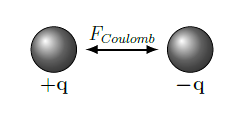
\includegraphics[scale=0.5]{image/chargecharge}	
\caption{Interaction électrostatique entre charges.}
\label{chargecharge}
\end{figure}



\begin{equation}
E_{Coulomb} = \frac{1}{4 \pi \epsilon_{0}} * \frac{q_{1} q_{2}}{r}
\end{equation}

\begin{flushleft}
\begin{tabular}{@{}lrp{10cm}}
avec & $q_{1}$ et $q_{2}$ : & charges respectives des particules 1 et 2, \\
& $r$ : & distance entre les particules. 
\end{tabular}
\end{flushleft}

L'induction est quant à elle due à la déformation de la densité électronique d'un atome ou d'une molécule par l'effet du champ électrique d'une molécule voisine. Ces deux contributions sont très bien définies en physique classique, contrairement à la dispersion et l'échange, qui sont liés à des effets quantiques.
En effet, ce sont les phénomènes de fluctuations quantiques de la distribution des charges qui sont à l'origine du terme de dispersion, et la contribution d'échange est dûe au principe d'exclusion de \textsc{Pauli} qui impose que deux électrons ne peuvent pas posséder le même état quantique au même moment. Dans le cas d'une paire d'atomes en interaction ayant leurs couches électroniques partiellement occupées, cette contribution est positive et engendre une liaison chimique liante forte. À l'inverse, lorsqu'il s'agit de systèmes électroniques à couche fermée, elle devient un terme de répulsion à courte distance responsable du phénomène d'exclusion stérique. Ce phénomène étant inclu dans la loi des \og gaz réels \fg{} de Van der Waals (équation~\ref{GR}) sous la forme du volume d'exclusion $nb$.  


D'une manière plus générale, c'est-à-dire en dépassant le cadre des gaz, les interactions de Van der Waals sont générées par les fluctuations de distributions de charge des atomes et molécules et conduisent aux équations suivantes, où l'énergie est exprimée en Joules :

\begin{align}
E_{Keesom} &= - \frac{1}{r^{6}} \left(\frac{\mu_{1}^{2}\mu_{2}^{2}}{3(4\pi \epsilon_{0} \epsilon)^{2} k_{B}T}\right) \\
E_{Debye} &= - \frac{1}{r^{6}} \left(\frac{\mu_{1}^{2}\alpha_{2}+\mu_{2}^{2}\alpha_{1}}{(4\pi \epsilon_{0} \epsilon)^{2}}\right) \\
E_{London} &= - \frac{1}{r^{6}} \left(\frac{3}{4}\frac{h\nu\alpha_{1}\alpha_{2}}{(4\pi \epsilon_{0})^{2}}\right)
\end{align}

\begin{flushleft}
\begin{tabular}{@{}lrp{10cm}}
avec & $\mu_{1}$ et $\mu_{2}$ : & moments dipolaires respectifs des particules 1 et 2, \\
& $\alpha_{1}$ et $\alpha_{2}$ : & polarisabilités respectives des particules 1 et 2, \\
& $\epsilon_{0}$ : & permittivité diélectrique du vide, \\
& $\epsilon$ : & permittivité diélectrique du milieu, \\
& $k_{B}$ : & constante de \textsc{Boltzmann}, égale à la constante des gaz parfaits $R$ divisée par le nombre d'\textsc{Avogadro} $\mathcal{N}\!a$, \\
& $T$ : & température, \\
& $r$ : & distance entre les particules. \\
\end{tabular}
\end{flushleft}

L'énergie de \textsc{Keesom} (effet d'orientation) représente l'énergie d'interaction entre deux dipôles électrostatiques, c'est-à-dire deux molécules ayant un moment dipolaire\footnote{Le moment dipôlaire d'une molécule résulte d'une répartition hétéroclite de charges électriques, telle que le barycentre des charges positives (noyaux) ne coïncide pas avec celui des charges négatives (électrons), les électrons étant en effet attirés par l'atome le plus électronégatif de la liaison.} $\mu{}$ non nul (figure~\ref{figKeesom}). Il s'agit concrètement de l'attraction mutuelle de deux dipôles permanents qui est d’autant plus forte que les moments dipolaires sont élevés (grande charge et petite taille de la molécule) et que la température est basse.

\begin{figure}[h]
\centering
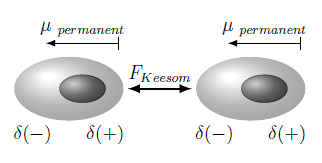
\includegraphics[scale=0.5]{image/Keesom}
\caption{Interaction entre dipôles électrostatiques.}
\label{figKeesom}
\end{figure}

Celle de \textsc{Debye} (effet d'induction) résulte de la déformation du nuage électronique d'une molécule, d'un atome ou d'un ion, par action du champ électrique engendré par le moment dipolaire d'une molécule voisine (figure \ref{figDebye}). Il en résulte ainsi un moment dipolaire induit. Elle est souvent nommé interaction dipôle {permanent-dipôle{ induit et fait intervenir le moment dipolaire $\mu$ et la polarisabilité\footnote{La polarisabilité est la capacité du nuage électronique à se déformer sous l'action d'un champ électrique. Le barycentre des charges négatives (électrons) étant légèrement décalé par rapport à celui des charges positives (noyaux) sous l'effet du champ, un moment électronique induit $\vec{m}_{e}$ apparaît, engendrant la notion de polarisabilité $\alpha$.} $\alpha$ des molécules concernées. Le nominateur $\mu_{1}^{2}\alpha_{2}+\mu_{2}^{2}\alpha_{1}$ décrit l'interaction lorsque les deux molécules sont polaires (cas A) mais s'écrit naturellement $\mu_{1}^{2}\alpha_{2}$ quand la seconde molécule est apolaire (cas B).

% mettre les deux cas dans la figure !
\begin{figure}[h]
\centering
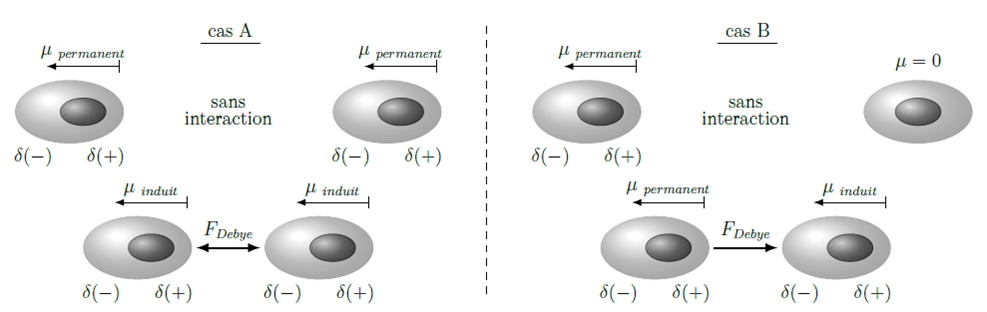
\includegraphics[scale=0.9]{image/Debye}
\caption{Interaction entre une molécule polaire et une seconde polarisable.}
\label{figDebye}
\end{figure}

Finalement, l'énergie de \textsc{London} (effet de dispersion), qui est la plus importante en terme de grandeur, représente l'interaction entre deux dipôles instantanés (figure \ref{figLondon}). Par définition, une molécule apolaire possède un moment dipolaire moyen nul mais la combinaison des mouvements des noyaux et des électrons fait qu'il existe malgré tout un moment dipolaire instantané. Cette interaction est d'autant plus forte que les deux molécules sont facilement polarisables, donc d'autant plus forte que leur taille est importante. Les forces de \textsc{London} étant présentes entre toutes les particules, quelle que soit leur nature, ce sont principalement elles qui permettent la cohésion de la matière dans l'univers.

Notons que les énergies de Van der Waals varient en fonction de l'inverse de la distance à l'ordre 6.

\begin{figure}[h]
\centering
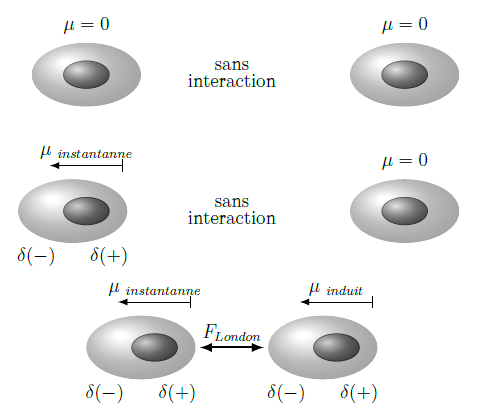
\includegraphics[scale=0.8]{image/London}
\caption{Interaction entre deux dipôles instantanés.}
\label{figLondon}
\end{figure}


Il existe toutefois d'autres types d'interactions électrostatiques que celles décrites par le modèle des forces de VdW. En effet, similaire dans l'esprit à l'énergie de \textsc{Keesom}, l'énergie d'interaction entre un ion et un dipôle permanent est donné par la formule suivante :

\begin{equation}
E_{ion-dipôle} = - \frac{1}{r^{2}} \frac{\mu_{1}q_{2}}{4\pi \epsilon_{0} \epsilon}
\end{equation} 

Il s'agit là encore de l'interaction positive entre une espèce chargée, anion ou cation, et une molécule possédant un moment dipolaire non-nul (\ref{figiondipole}). Ce phénomène est notamment à l'origine de la dissolution des espèces ioniques (ex~:~NaCl) dans un solvant polaire, de l'étape de solvatation qui suit, puis de la bonne dispersion des charges en solution.

\begin{figure}[h]
\centering
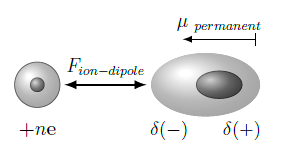
\includegraphics[scale=0.7]{image/Ion-dipole}
\caption{Interaction entre une espèce chargée et une molécule polaire.}
\label{figiondipole}
\end{figure}

De plus, notons aussi la spécificité de la liaison hydrogène qui est une liaison chimique non covalente, de type dipôle-dipôle. Lorsqu'un hétéroatome possédant au moins une paire libre est suffisamment électronégatif (ex : O, N, F), il vient se positionner aux abords d'un hydrogène acide porté par un autre atome fortement électronégatif afin d'en stabiliser la charge partielle $\delta (+)$ ainsi créée.

Bien que de la même famille que les forces de Van der Waals, \textit{i.e.} électrostatique, les liaisons hydrogènes s'en distinguent par une intensité environ dix fois supérieure. Elles restent toutefois une vingtaine de fois plus faibles qu'une liaison covalente. La distance moyenne entre les deux hétéroatomes est de l'ordre de 2,5 \AA .

Dans le cadre de cette thèse, ce sont principalement les interactions entre systèmes conjugués, \textit{i.e.} interactions $\pi-\pi$, qu'il sera nécessaire de traduire. Comme nous pouvons le voir dans le cas simple d'un dimère de benzène représenté en figure \ref{pistackbenz}, l'interaction positive se fait entre les liaisons $\sigma$ et les liaisons $\pi$ alors que les nuages électroniques des liaisons $\pi$ se repoussent naturellement, dû à leurs charges négatives.

Notons que nous retrouvons ce phénomène sous des aspects intramoléculaires, comme par exemple dans le cas de l'hyperconjugaison $\sigma-\pi$ qui vient stabiliser certaines conformations du toluène.

\begin{figure}[h]
\centering
\begin{tikzpicture}[scale=0.7, every node/.style={scale=0.7}]
\shade [shading=ball, ball color=gray, opacity=0.5] (0,0.8) ellipse (2.2cm and 0.6cm) ;
\draw (-2,1.2) --++ (1,0.5) --++ (2,0) --++ (1,-0.5) ;
\fill (-2,1.2) --++ (1,-0.6) --++ (2,0) --++ (1,0.6) --++ (-1,-0.5) --++ (-2,0) -- cycle ;
\draw [dashed] (0,1.2) ellipse (1.4cm and 0.35cm) ;
\shade [shading=ball, ball color=gray, opacity=0.5] (0,1.6) ellipse (2.2cm and 0.6cm) ;
\shade [shading=ball, ball color=gray, opacity=0.5] (0,-1.6) ellipse (2.2cm and 0.6cm) ;
\draw (-2,-1.2) --++ (1,0.5) --++ (2,0) --++ (1,-0.5) ;
\fill (-2,-1.2) --++ (1,-0.6) --++ (2,0) --++ (1,0.6) --++ (-1,-0.5) --++ (-2,0) -- cycle ;
\draw [dashed] (0,-1.2) ellipse (1.4cm and 0.35cm) ;
\shade [shading=ball, ball color=gray, opacity=0.5] (0,-0.8) ellipse (2.2cm and 0.6cm) ;
\draw [latex-latex, thick] (-2.2,-1.2) ..controls +(-1.7,0) and +(-1.5,0).. (-2.4,0.8) node [above, midway, rotate=90, yshift=3mm] {interaction attractive $\sigma - \pi$} ;
\draw [latex-latex, thick] (-2.2,1.2) ..controls +(-1.7,0) and +(-1.5,0).. (-2.4,-0.8) ;
\draw [latex-latex, thick] (2.4,-0.8) ..controls +(1.5,0) and +(1.5,0).. (2.4,0.8) node [below, midway, rotate=90, yshift=-2mm] {interaction répulsive $\pi - \pi$} ;
\end{tikzpicture}
\caption{$\pi$-stacking dans le cas d'un dimère de benzène}
\label{pistackbenz}
\end{figure}

Même si la théorie de la fonctionnelle de la densité connaît un large succès tant elle arrive désormais bien à traduire les phénomènes de liaisons chimiques, les structures géométriques et même la cohésion des solides moléculaires et cristallins, il reste toujours l'obstacle des systèmes chimiques où les forces de Van der Waals sont prédominantes. En effet, les effets de corrélation électronique des forces de dispersion étant purement non-locaux, l'approximation locale ou non-locale qui fait le fondement de la DFT restera problèmatique. Se pose alors la question de savoir comment modéliser ces types d'interaction de façon idiomatique. Nous allons voir que l'élaboration d'une fonctionnelle hybride à longue portée est capable de répondre à cette problèmatique.

\section[LC-DFT-D hybride : $\omega$BXD]{Construction d'une LC-DFT-D hybride : cas de la $\omega$BXD}

Les DFT hybrides avec correction à longue portée basées sur la théorie \textsc{Kohn-Sham} ont naturellement rencontré un grand engouement puisque la précision apportée n'accroît pas le coût calculatoire par rapport aux DFT hybrides.

\subsection{B88}

Comme nous l'avons vu dans le cadre des approximations de la fonctionnelle de la densité, notées DFAs\footnote{\og Density Functional Approximations \fg{} }, la décroissance en exponentielle du potentiel d'échange-corrélation, au lieu d'être en $1/r$, engendre une mauvaise représentation des interactions à longue distance. Cette erreur, nommée erreur d'auto-interaction (SIE, pour \og self-interaction error \fg{}), est liée au fait que ces approximations, basées sur la densité de spin locale (LSDA, pour \og local spin density approximation \fg{}), décrivent mal l'état fondamental qui devrait être, dans le cadre de la DFT pure, strictement sans auto-interaction.     
C'est pourquoi, afin d'introduire un effet non-local de l'échange-corrélation dans le modèle KS-DFT (partie~\ref{Kohn-Sham}), \textsc{Becke} proposa en 1988 d'incorporer dans sa fonctionnelle d'échange B88~\cite{becke1988density} une petite part d'echange exact \textsc{Hartree-Fock}. 

Dans le cadre général des DFAs, l'énergie d'échange-corrélation s'écrit donc :

\begin{equation}
E_{xc} = c_{x}E_{x}^{HF} + E_{xc}^{DFA}
\label{xcB88}
\end{equation}

\noindent où $c_{x}$ prend généralement des valeurs comprises entre 0,2 et 0,25~\cite{becke1993density} pour les données thermodynamiques et entre 0,4 et 0,6~\cite{boese2004development} pour les études cinétiques.

Basée sur ce modèle, la désormais bien connue DFT hybride B3LYP \cite{becke1993density} (équation~\ref{B3LYP}) donne des résultats comparables à ceux obtenus à partir de la théorie perturbative \textsc{M\o ller-Plesset} à l'ordre 2 \cite{moller1934note}, noté MP2, souvent utilisée comme référence, dans le cadre de systèmes fortement liés. Depuis, de nombreuses recherches ont porté sur l'amélioration constante de ce potentiel d'échange-corrélation $E_{xc}[\rho]$.

\subsection{B97}

Une avancée significative a de nouveau été faite par \textsc{Becke} en 1997 dans le domaine des KS-DFT. Par une méthode similaire à la combinaison linéaire d'orbitales atomiques, notée LCAO\footnote{\og Linear Combination of Atomic Orbitals \fg{}.}, il a proposé un modèle mathématique basé sur l'approximation de densité de spin local (LSDA), sa première dérivée et une petite fraction d'échange HF pour décrire le potentiel d'échange-corrélation $E_{xc}[\rho]$. Une optimisation systématique des coefficients linéaires à partir d'un jeu classique de données expérimentales a conduit à l'apparition de la méthode B97~\cite{becke1997density}. La base de données contient notamment des valeurs relatives à l'interaction entre systèmes conjugués.

Cette méthodologie a été reprise par F. A. \textsc{Hamprecht} et al, P. J. \textsc{Wilson} et al et T. W. \textsc{Keal} et al pour respectivement conduire à la B97-1 \cite{hamprecht1998development} (1998), la B97-2 \cite{wilson2001hybrid} (2001) et la B97-3 \cite{keal2005semiempirical} (2005). Il s'agissait alors de réoptimisations des coefficients linéaires par rapport à d'autres bases de données expérimentales plus complètes.

Mais cette reparamétrisation empirique du terme d'échange-corrélation ne résout pas le problème de sa non-décroissance en $1/r$. La prise en compte totale du terme d'échange HF $E_{x}^{HF}$ ($c_{x}$=1 dans l'équation~\ref{xcB88}) pourait résoudre ce problème mais cela serait incompatible avec le terme de corrélation DFA $E_{c}^{DFA}$. En effet, il existerait alors une mauvaise compensation des erreurs respectives.

\subsection{$\omega$B97}

L'idée de séparer le traitement des interactions courtes (SR, pour \og short range \fg{}) et longues portées (LR, pour \og long range \fg{}) s'est alors présentée comme le choix le plus évident, aussi bien au niveau de la compréhension des phénomènes que mathématiquement parlant. Nous pouvons ainsi traiter séparément à l'aide d'une fonction erreur $(erf)$ les interactions à courtes distances par une fonctionnelle de la densité et celles longue distance par une fonction d'onde. Ce principe conduit naturellement à l'élaboration d'une fonctionnelle hybride à séparation de portée. L'introduction de la fonction erreur, avec un paramètre libre, permet de contrôler le rayon d'action des interactions de courte-portée.

La première proposition faite par \textsc{Iikura} et al \cite{iikura2001long} a été de traiter la partie d'échange LR par la théorie HF alors que la partie SR est approximée par une DFA; le terme de corrélation est quant à lui le même que celui de \textsc{Coulomb}, quelle que soit la distance :

\begin{equation}
E_{xc}^{LC-DFA} = E_{x}^{LR-HF} + E_{x}^{SR-DFA} + E_{c}^{DFA}
\end{equation}

Ce schéma de séparation de portée a l'avantage de conduire à des temps de calcul très proches des DFT hybrides, mais il reste à développer une fonctionnelle d'échange SR précise et une fonctionnelle de corrélation qui soit entièrement compatible entre elles.

Le type d'opérateur de coupure le plus utilisé dans le cadre des LC-DFT hybrides est la fonction d'erreur standard $(erf)$ :

\begin{equation}
\frac{1}{r} = \frac{erf(\omega r_{12})}{r_{12}} + \frac{erfc(\omega r_{12})}{r_{12}}
\label{erf}
\end{equation}

\begin{flushleft}
\begin{tabular}{@{}lrp{10cm}}
avec & $\frac{erf(\omega r_{12})}{r_{12}}$ : & interaction de courte portée, \\
& $\frac{erfc(\omega r_{12})}{r_{12}}$ : & interaction complémentaire, \\
& $r_{12}$ : & distance entre les particules 1 et 2, \\
& $\omega$ : & paramètre contrôlant la séparation.
\end{tabular}
\end{flushleft}

Notons que l'introduction du paramètre $\omega$, qui s'exprime comme l'inverse d'une distance, permet de donner un sens physique à cette valeur, en cela qu'il est étroitement lié à une longueur caractéristique de la séparation.
Naturellement, il existe différents types de fonctions erreur $(erf)$ afin de faciliter son intégration mathématique dans les codes de calculs. Dans le cas de la $\omega$B97 \cite{chai2008long} et, par conséquent, des fonctionnelles $\omega$B97X et $\omega$B97X-D, c'est la fonction $erf/erfc$ qui a été choisie par Jeng-Da \textsc{Chai} et Martin \textsc{Head-Gordon} dans leurs travaux. \\

Le choix des auteurs s'est porté sur un terme d'échange exact HF longue portée $E_{x}^{LR-HF}$, calculé à partir des spin-orbitales occupées $\phi_{i \sigma}(r)$, et une forme analytique du terme d'échange $E_{x}^{SR-DFA}$ obtenue par l'intégration du carré de la matrice densité LSDA :

\begin{align}
E_{x}^{LR-HF} &= -\frac{1}{2} \sum_{\sigma} \sum_{ij}^{occ.} \iint \phi_{i \sigma}^{*}(r_{1}) \phi_{j \sigma}^{*}(r_{1}) \frac{erf(\omega r_{12})}{r_{12}} \phi_{i \sigma}(r_{2}) \phi_{j \sigma}(r_{2}).dr_{1}.dr_{2}, \\
E_{x}^{SR-LSDA} &= \sum_{\sigma} \int \underbrace{-\frac{3}{2}\left(\frac{3}{4\pi}\right)^{1/3}\rho_{\sigma}^{4/3} (r) F(a_{\sigma})}_{e_{x \sigma}^{SR-LSDA} (\rho_{\sigma}) .dr}.
\end{align}

\noindent où :
\begin{align}
k_{F \sigma}&=(6\pi^{2}\rho_{sigma}(r))^{1/3},\nonumber\\
F(a_{\sigma})&=1-\frac{8}{3}a_{\sigma}\left[\sqrt{\pi}\: erf\left(\frac{1}{2a_{\sigma}}\right)-3a_{\sigma}+4a_{\sigma}^{3}+(2a_{\sigma}-4a_{\sigma}^{3}) \: exp\left(-\frac{1}{4a_{\sigma}^{2}}\right)\right],\nonumber\\
a_{\sigma}&=\frac{\omega}{2k_{F\sigma}}.\nonumber
\end{align}

\begin{flushleft}
\begin{tabular}{@{}lrp{10cm}}
avec & $k_{F\sigma}$ : & vecteur d'onde local de Fermi,\\
& $F(a_{\sigma})$ : & fonction d'atténuation,\\
& $a_{\sigma}$ : & paramètre de contrôle (sans unité) de la fonction d'atténuation $F(a_{\sigma})$.
\end{tabular}
\end{flushleft}

En retenant une fonctionnelle de corrélation basée elle aussi sur la LSDA $E_{c}^{LSDA}$, la plus simple des DFT hybrides à correction de longue portée (RSHX-LDA) s'écrit~:

\begin{equation}
E_{xc}^{RSHXLDA} = E_{x}^{LR-HF} + E_{x}^{SR-LSDA} + E_{c}^{LSDA}
\end{equation}

La fonctionnelle $\omega$B97\cite{chai2008long} s'écrit alors :

\begin{equation}
E_{xc}^{\omega B97} = E_{x}^{LR-HF} + E_{x}^{SR-B97} + E_{c}^{B97}
\end{equation}

Il est à noter que celle-ci ne possède pas d'échange \textsc{Hartree-Fock} à courte portée (SR), comme la plupart des fonctionnelles hybrides à correction de portée.

Malgré plusieurs études visant à optimiser la valeur du paramètre $\omega$, la précision calculatoire reste insuffisante en terme de thermochimie. En effet, nous l'avons déjà vu, une valeur trop grande pour $\omega$ tendrait vers une incompatibilité entre le terme d'échange non-local $E_{x}^{LR-HF}$ et le terme local de corrélation $E_{c}^{LSDA}$. De plus, nous pouvons aisément comprendre, d'après l'équation~\ref{erf}, que plus $\omega$ est petit, plus la contribution du terme d'échange SR $E_{x}^{SR-LSDA}$ sera importante. L'utilisation d'une trop faible valeur  reviendrait alors à traiter le problème dans un cadre très proche de la LDA classique qui, comme nous l'avons vu dans la partie~\ref{lda}, est incapable de traduire correctement le terme d'échange à courte portée.

\subsection{$\omega$B97X}

Afin d'y remédier, une partie d'échange SR HF $E_{x}^{SR-HF}$, est ajoutée à $E_{x}^{SR-LSDA}$ dans une proportion d'environ 16\%,  de la même manière que \textsc{Becke} dans la fonctionnelle B88. Ceci à l'avantage de ne pas perturber la partie LR qui est dorénavant correcte. Ainsi, la nouvelle fonctionnelle comporte désormais un paramètre $c_{x}$ contrôlant la proportion d'échange exact HF à courte distance, comme nous pouvons le voir dans son expression :

\begin{equation}
E_{xc}^{LC-DFA} = E_{x}^{LR-HF} + c_{x}E_{x}^{SR-HF} + E_{x}^{SR-DFA} + E_{c}^{DFA}
\end{equation}

\noindent où :

\begin{equation}
E_{x}^{SR-HF} = -\frac{1}{2} \sum_{\sigma} \sum_{ij}^{occ.} \iint \phi_{i \sigma}^{*}(r_{1}) \phi_{j \sigma}^{*}(r_{1}) \frac{erfc(\omega r_{12})}{r_{12}} \phi_{i \sigma}(r_{2}) \phi_{j \sigma}(r_{2}).dr_{1}.dr_{2}, \\
\end{equation}

C'est ainsi que la fonctionnelle $\omega$B7X\cite{chai2008long} se décompose de la façon suivante~:

\begin{equation}
E_{xc}^{\omega B97X} = E_{x}^{LR-HF} + c_{x}E_{x}^{SR-HF} + E_{x}^{SR-B97} + E_{c}^{B97}
\end{equation}

La valeur de $\omega$, comme les valeurs des coefficients de développements linéaires et de développements à l'ordre $m$ des fonctionnelles $\omega$B97 et $\omega$B97X ont été déterminées par la méthode des moindres carrés appliquée à une base de données composées de 412 valeurs précises, expérimentales et théoriques.

Malgré toutes ces optimisations conduisant à une bien meilleure représentation des systèmes en interaction, ces fonctionnelles connaissent encore des lacunes quant à la traduction des interactions de dispersion entre atomes, ie les forces de \textsc{London}. Comme nous allons le voir dans le cas de la fonctionnelle $\omega$B97X-D, ceci peut être corrigé par une prise en compte empirique des effets de dispersion.

\subsection{$\omega$B97X-D}

Cette dernière correction pourrait naturellement passer par le calcul idiomatique de l'énergie de dispersion entre chaque atome, mais cela occasionnerait alors un coût calculatoire prohibitif. C'est pourquoi Jeng-Da \textsc{Chai} et Martin \textsc{Head-Gordon} ont fait le choix d'appliquer cette correction de façon empirique par l'ajout d'un terme $E_{disp}$ à la fonctionnelle KS-DFT, ici la $\omega$B97X. L'expression de l'énergie de la fonctionnelle $\omega$B97X-D \cite{chai2008long} ainsi créée devient alors :

\begin{equation}
E_{DFT-D}=E_{\omega B97X}+E_{disp}
\end{equation}

L'énergie de dispersion $E_{disp}$ est définie par rapport à une fonction d'amortissement $f_{damp}$ :

\begin{equation}
E_{disp}=-\sum_{i-1}^{N_{at}-1} \sum_{j-i+1}^{N_{at}} \frac{C_{6}^{ij}}{R_{ij}^{6}}f_{damp} (R_{ij})
\end{equation}

\noindent où :
\begin{equation}
f_{damp} (R_{ij})=\frac{1}{1+a(\frac{R_{ij}}{R_{r}})^{-12}}
\end{equation}

Une nouvelle fois, la partie empirique a été paramétrée par rapport à la même base de données que pour les fonctionnelles $\omega$B97 et $\omega$BX97.


\newpage

\section*{Conclusion}
\markright{CONCLUSION}{}

En résumé, l'apport de la fonction erreur $(erf)$ permet de mieux gérer les contributions d'échange-corrélation selon la distance d'interaction. Les DFT hybrides $\omega$B97 et $\omega$B97X prennent ainsi en compte la totalité de l'échange exact à longue distance et utilisent la méthode des gradients généralisés à faible distance, alors que la corrélation électronique reste basée sur celle initialement développée par \textsc{Becke} dans la fonctionnelle B97. Ceci a pour effet de supprimer le problème d'auto-interaction de la fonctionnelle d'échange à longue distance.

Les travaux de Jeng-Da \textsc{Chai} et Martin \textsc{Head-Gordon} ont finalement conduit à la fonctionnelle $\omega$B9X-D, de type LC-DFT-D hybride, où la totalité de l'échange exact HF est pris en compte à longue distance, en même temps qu'une petite partie -- environ 22 \% -- de l'échange exact HF est introduite à courte distance pour compléter une fonctionnelle d'échange B97 modifiée ; une correction empirique de la dispersion est finalement appliquée.

Comme toutes les fonctionnelles LC-DFT, le problème de l'auto-interaction est corrigé à longue distance mais reste quelque peu présent à courte distance. Les effets de corrélation à longue distance sont quant à eux purement et simplement traités par la correction empirique de dispersion.

Cette fonctionnelle est, d'après les tests des auteurs, définitivement plus adaptée à l'étude de systèmes chimiques où les interactions non-covalentes sont importantes.







%\newgeometry{textwidth=16cm}
\chapter[Corrections à la dispersion]{Corrections à la Dispersion}
\minitoc
\restoregeometry

\newpage

	\section*{Introduction}
\spacing{1.5}
	
	En mécanique quantique les molécules sont décryptes comme un assemblage de noyaux et d'électrons attaché aux effets classiques et quantiques. Même en considérant les noyaux comme fixes, le comportement des électrons constituent un problème complique à N corps. Pour la résolution de l'équation de Schrödinger la théorie de la fonctionnelle de la densité établie une alternative intéressante pour aborder ce problème, grâce à la description du système par sa densité électronique\cite{adamo2014decrire}.
	
	\bigskip
	La DFT a eu un grand succès dans l'étude de systèmes dans lesquels la taille fait impossible un calcul ab initio Post Hartree- Fock, pour la compréhension parmi différents sujets en sciences et technologie.\cite{neese2009prediction,sanchez1997density,waller2006hybrid}
	\bigskip
	
	Cependant cette méthode présente déficiences au moment de traduire la dispersion dans les systèmes et les interactions du van der Waals, voire le théorème Hohenberg- Kohn prédit que si nous connaissons la fonctionnelle correcte, nous pourrions obtenir l’énergie à l’état fondamental en arrivant à son point minimum, donc la difficulté provient des fonctionnelles approximatifs. Local et semi local fonctionnelles  ne peuvent pas reproduire le comportement asymptotique de $1/R^{6}$, comme cela affecte les molécules où il y a une considérable superposition de la densité est inconnue. Il existe une corrélation claire de l'incapacité de décrire les interactions de Van der Waals avec la fonctionnelle d'échange GGA dans la région de faible densité et gradient de densité réduite x. 
	
	\bigskip
	
	L'échec de LDA et GGA pour donner l'énergie correcte pour deux densités fixes a longue distances a conduit à des corrections, surtout dans l'étude des interactions intermoléculaire qui définissent le comportement de systèmes complexes en chimie et biologie. 
	
	Ce chapitre constitue l'occasion de connaitre les bases des corrections disponibles pour les calculs électroniques et qui nos aideront à avoir une approche théorique plus exacte dans les interactions des heterocycles aromatiques.  
	
	\newpage
	
	\section{DFT-D2}
	
	En 2006 Stefan Grimme \cite{grimme2006semiempirical} propose une correction à la dispersion basée en semiempirical GGA adjustement de la correction déjà présenté pour lui même en 2004 \cite{grimme2004accurate}, dû à l'amélioration de trois points : 
	
	\begin{itemize}
		\item Les coefficients C$_{6}$ étaient disponibles que pour les premières atomes du tableau périodique.
		\item Calculs d'essaie pour molécules avec atomes du troisième période ont montré des erreurs systématiques. 
		\item L'addition de l'énergie de dispersion à l'énergie KS-DFT conduit a des incohérences pour les valeurs normaux en thermochimie. 
	\end{itemize} 
	
	\subsection{Theorie}
	
	L'approche est basée dans la fonctionnelle de Becke (GGA) \cite{becke1997density}. La fonctionnelle B97 est fondée : 
	
	\begin{equation}
	S_{\sigma} = \frac{\bigtriangledown n_{\sigma}}{n_{\sigma}^{4/3}}
	\end{equation}
	 
	 Où n est la densité électronique et $\sigma$ dénote le spin ($\alpha ou \beta$ selon la position). La partie de la densité qui dépende de l'échange-corrélation vient donnée par :
	 
	 \begin{equation}
	 E_{XC} = E_{X} + E_{C\alpha \beta} + \sum_{\sigma} E_{C\sigma \sigma}
	 \end{equation}
	
	Où X et C sont les contributions d'échange et corrélation respectivement. 
	
	L'énergie total est : 
	
	\begin{equation}
	E_{DFT-D} = E_{KS-DFT} + E_{disp}
	\end{equation}
	
	Où $E_{KS-DFT}$ est l'énergie KS usuel obtenue par la fonctionnelle de la densité choisie, et $E_{disp}$ est la correction à la dispersion qui est représente par :
	
	\begin{equation}
	E_{disp}= -s_{6} \sum_{i=1}^{N_{at-1}} \sum_{j=i+1}^{N_{at}} \frac{C_{6}^{ij}}{R_{ij}^{6}} f_{dmp} (R_{ij})
	\end{equation}

  $N_{at}$ est le nombre des atomes dans le système, $C_{6}^{ij}$ le coefficient de la dispersion pour les atomes paire ij, $s_{6}$ est le scaling facteur qui dépende de la fonctionnelle choisie pour le calcul DFT et $R_{ij}$ est la distance interatomique. 
  
  Les paramètres $C_{6}$ ($Jnm^{6}mol^{-1}$) et $R_{0}$ ($\AA$) radio de van der Waals utilisés dans le champ de force semiempirique de Grimme sont tabulé, selon la figure \ref{Grimme-parametres}. 
  
  \begin{figure}[H]
  	\centering
  	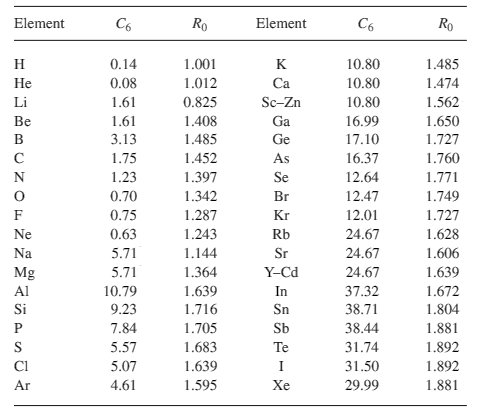
\includegraphics[scale=0.8]{image/C6}
  	\caption[Les paramètres empiriques $C_{6}$ et $R_{0}$ pour DFT-D2]{Les paramètres $C_{6}$ et $R_{0}$} \label{Grimme-parametres}
  \end{figure}
	

	La correction D2 a été employé par Grimme \cite{grimme2006semiempirical} dans systèmes de références comme gaz diatomiques, benzène, anthracène, etc. Les clusters du deuxième groupe du tableau périodique ont donné les plus grands erreurs à cause de la difficile description de systèmes avec cette configuration électronique, laquelle donné des interactions type métalliques.  
	
	Park et al \cite{park2011ab} étudient l'interaction benzène-benzène dans le cas graphite, ils ont trouvé bon corrélation avec les données expérimentales pour les paramètres de maille. 
	
	Plus tard Lee et al \cite{lee2013sum} rapportent les fréquences de vibration des polymorphes de cellulose $I_{\alpha}$ et $I_{\beta}$ dans le logiciel VASP, cependant le valeur du streching OH calculé est 100 cm$^{-1}$ plus petit que l'expérimental. 
	
	
 	\section{DFT-D3}
	
	Les propriétés que présente cette correction par rapport aux versions précédents sont les suivantes :
	\bigskip 
	\begin{itemize}
		\item Elle est moins empirique, les paramètres les plus importants sont calculés par KS-DFT.
		\item L'approche est asympotiquement corrigée pour les fonctionnelles de la densité dans les systèmes limités (molécules) ou systèmes infinites non métalliques.
		\item Elle fournit une description pour les éléments plus relevants (Z=1-94).
		\item Les coefficients de la dispersion des atomes paires et leur cutoff radio sont calculés. 
	\end{itemize}
	\bigskip
	
	L'énergie totale DFT-D3 est donnée par la relation:	
	\begin{equation}
	E_{DFT-D3} = E_{KS-DFT} - E_{disp}
	\end{equation} 
	\bigskip
	
	Où $E_{KS-DFT}$ est l'énergie KS usuel obtenue par la fonctionnelle de la densité choisie, et $E_{disp}$ est la correction à la dispersion qui est représente comme une somme de l'énergie de deux ou trois corps.
	
	\begin{equation}
	E_{disp} = E ^{(2)} + E^{(3)}
	\end{equation}
	
	Le plus important terme de deux corps expression est :
	\begin{equation}
	E^{(2)} = \sum_{AB} \sum_{n=6,8,10...} s_{n}\frac{C_{n}^{AB}}{r^{n}_{AB}} f_{d,n} (r_{AB})
	\end{equation}
	Le premier somme est sur tous les atomes paires du systèmes. $C_{n}^{AB}$ indique la moyenne de nème ordre des coefficients de la dispersion pour les atomes paires AB, et $r_{AB}$ est la distance internucléaire entre eux. Global $s_{n}$ ou facteur d'écaillage est ajusté seulement pour $n>6$ pour assurer l'exactitude asymptotique qui est remplie quand $C_{6}^{AB}$ est exacte. 
	\bigskip
	
	$C_{6}$ terme n'est pas largement écaillage, les plus hauts termes sont nécessaires afin d'adapter le potentiel pour la fonctionnelle de la densité utilisée dans sa région moyenne. Il a été constaté que les termes $n>8$ fassent la méthode légèrement instable dans certains situations, pour cela il a été fait une troncature à $n=8$.
	\bigskip
	
	Pour éviter les singularités dans petits $r_{AB}$ et double comptage des effets de corrélation pour distances intermédiaires, la fonction damping $f_{d,n}$ est employée pour déterminer le range de la correction de la dispersion.
	\bigskip
	
	Il est utilisé une variante proposée par Chai et Head-Gordon\cite{chai2008long} laquelle révèle être numériquement stable et pratique également pour les termes d'ordre supérieur de la dispersion. l'expression de cette fonction est donnée par :
	
	\begin{equation}
	f_{d,n} (r_{AB}) = \frac{1}{1+ 6(r_{AB}/(s_{r,n}R_{0}^{AB}))^{-\alpha_{n}}}
	\end{equation}
	\bigskip
	
	Où $s_{r,n}$ est le facteur d'écaillage dépendant du radio de cutoff $R_{0}^{AB}$. Il remplace $s_{6}$ terme en DFT-D2. 
	\bigskip
	
	Compare au potentiel DFT-D2 le nouveau est moins contraignant pour les petites distances
	mais plus attrayante dans la région typique des interactions de van der waals. Il fournit une séparation plus nette entre le court terme et les effets de dispersion à longue portée.
	
	\subsection{Les coefficients de la dispersion}
	
	
	Au lieu d'utiliser une formule d'interpolation dérivée de manière empirique comme dans DFT-D2, les coefficients de la dispersion sont maintenant calculés par DFT dépendant du temps (TD-DFT), employant des relations de récursion connues pour les termes d'ordre supérieur des multipôles. Le point du départ est la formule de Casimir- Polde\cite{kaplan2006intermolecular} 
	
	\bigskip
	\begin{equation}
	C_{6}^{AB} = \frac{3}{\pi}\int_{0}^{\infty} \alpha^{A} (i\omega) \alpha^{B} (i\omega) d\omega
	\end{equation}
	\bigskip
	
	Où $\alpha(i\omega)$ est la moyenne du dipôle de polarisabilité à la fréquence imaginaire $\omega$. Les coefficients d'ordre supérieur sont calculés récursivement par :
	\bigskip
	\begin{equation}
	C_{8}^{AB} = 3C_{6}^{AB} \sqrt{Q^{A}Q^{B}}
	\end{equation}
	
	et \begin{equation}
	C_{10}^{AB} =\frac{49}{40} \frac{(C_{8}^{AB})^{2}}{C_{6}^{AB}}
	\end{equation}
	
	Avec
	\begin{equation}
	Q^{A} = s_{42}\sqrt{Z^{A}} \frac{\langle r^{4}\rangle r^{A}}{\langle r^{2}\rangle r^{A}}
	\end{equation}
	
	\bigskip
	\subsection{Le terme de Trois Corps}
	\bigskip
	
	La partie à long terme de l'interaction entre trois atomes à l'état fondamental ne correspond pas exactement aux énergies d'interaction prises par paires. Au meilleur de nos connaissances, nous ne sommes pas conscients de toute considération de cet effet dans une structure modèle. Le premier terme non additif de dispersion dérivé du
	la théorie des perturbations de troisième ordre pour trois atomes ABC est :
	
	\begin{equation}
	E^{ABC} = \frac{C_{9}^{ABC}(3\cos\theta_{a}\cos\theta_{b}\cos\theta_{c}+ 1)}{(r_{AB} r_{BC} r_{CA})^{3}}
	\end{equation}
	
	
	Reckien et al \cite{reckien2012implementation} ont mis en place dans le logiciel VASP les corrections D2 et D3. Ils ont étudié métaux, oxydes métalliques, cristaux moléculaires comme benzène, et l'adsorption sur surfaces. Tous les deux méthodes montrent qualitatif et quantitatif resultats des paramètres de maille, cependant la méthode D3 proportionne une meilleure performance.   
	
	\bigskip
	\section{La méthode Tkatchenko-Scheffler (DFT-TS)}
	
	Elle a été propose en 2009 par Tkatchenko et Scheffler\cite{tkatchenko2009accurate}. Nombreux études des structures cristallines ont été menés en utilisant cette correction. Par exemple Kronik et Tkatchenko\cite{kronik2014understanding} étudient le cristal d'Hemozoin d'importance biologique, lequel présent des interactions sur les liaisons hydrogènes. Pour vérifier l'exactitude de la méthode ils sont calculés les paramètres de maille et les modes de vibration du Brushite et le phosphate de calcium hydraté. Bu\u{c}ko et col\cite{buvcko2014extending} ont montre que la méthode peut être utilisée dans systèmes ioniques en changeant le calcul de volume effectif et les charges des atomes par la version itératif de la partition de Hisrfeld.
	
	Dans cette méthode la expression pour l'énergie de dispersion est officiellement identique à la méthode DFT-D2, la plus important différence cependant c'est que les coefficients de dispersion et la fonction damping sont dépendants de la densité de charge. La méthode DFT-TS est capable de prendre en compte les variation à la contribution des interactions de van der waals des atomes dû à leur environnement. 
	
	En effet les coefficient de la dispersion, la polarisabilité et les radios atomiques sont calculés à partir des valeurs des atomes libres selon les expressions suivantes :
	
	\begin{equation}
	\alpha_{i} = \nu_{i} \alpha_{i}^{free}
	\end{equation}
	
	\begin{equation}
	C_{6ii} = \nu_{i}^{2} C_{6ii}^{free}
	\end{equation}
	
	\begin{equation}
	R_{0i} = \left(\frac{\alpha_{i}}{\alpha_{i}^{free}}\right)^{\frac{1}{3}} R_{0i}^{free}
	\end{equation}
	
	Les paramètres $\alpha_{i}^{free}$, $C_{6ii}^{free}$ et $R_{0i}^{free}$ sont tabulé pour tous les éléments des premiers 6 lignes du tableau périodique des éléments, sauf pou les lanthanides. $\nu_{i}$ représente le volume effectif et il est calculé en utilisant la partition de Hirshfeld de la densité des électrons. 
	
	\begin{equation}
	\nu_{i} = \frac{\int r^{3} w_{i}(r)n(r)d^{3}r}{\int n_{i}^{free} (r)d^{3}r}
	\end{equation}
	
	Où n(r) est la densité totale électronique, $n_{i}^{free}$ est la moyenne de la densité électronique sphérique des électrons pour les espèces atomiques neutres libres i. $w_{i}(r)$ est le poids de Hisrfeld et il se définit par les densités atomiques libres.
	
	\begin{equation}
	w_{i}(r)= \frac{n_{i}^{free}(r)}{\sum_{j=1}^{N} n_{j}^{free}(r)}
	\end{equation}
	\bigskip
	
	L'energie de dispersion su système AB est égal : 
	
	\begin{equation}
	E_{dis}= -\frac{1}{2} \sum_{A=1}^{N} \sum_{B=1}^{N} \sum_{L} \frac{C_{6AB}}{R^{6}_{AB,L}} f_{damp}(R_{AB,L})
	\end{equation}
	\bigskip
	
	\subsection{Self-consistent screening dans la méthode Tkatchenko-Scheffler}
	
	Ce variant de la méthode Tkatchenko-Scheffler a été proposé en 2012 par Tkatchenko et col\cite{tkatchenko2012accurate} avec l'objectif d'inclure le dépistage des effets à longe portée des polarisabilités effectifs des atomes. Grâce à l'utilisation de l'équation self-consistent screening d'électrodynamique classique. 
	
	Cela conduit à une description clair de polarisation et dépolarisation pour le tenseur de polarisabilité des molécules et solides. 
	
	Dans cette méthode la fréquence dépendante de la polarisabilité s'obtient la équation self-consistent :
	
	\begin{equation}
	\alpha_{i^{SCS}}(\omega) = \alpha_{i}(\omega) - \alpha_{i}(\omega) \sum_{i\neq j} \tau_{ij} \alpha_{j}^{SCS}(\omega)
	\end{equation} 
	
	où $\tau_{ij}$ est le tenseur d'interaction dipôle- dipôle et $\alpha_{i}(\omega)$ est la fréquence effectif dépendant de la polarisabilité, avec l'expression approximatif : 
	
	\begin{equation}
	\alpha_{i} (\omega) = \frac{\alpha_{i}}{1 + (\omega/\omega_{i})^{2}}
	\end{equation}
	
	avec la fréquence d'excitation moyenne caractéristique $\omega_{i} = \frac{4}{3} \frac{C_{6ii}}{(\alpha_{i})^{2}}$
	\bigskip
	
	Les coefficients de la dispersion sont calcules par l'intégral de Casimir- Polder :
	
	\begin{equation}
	C_{6ii} = \frac{3}{\pi} \int_{0}^{\infty} \alpha_{i}^{SCS} (\omega) \alpha_{i}^{SCS} (\omega) d\omega
	\end{equation}
	
	Les radios atomiques de van der waals sont calcules par renormalisation du radio obtenu par la méthode de Tkatchenko (DFT-TS). 
	
	\begin{equation}
	R_{0i}^{SCS} = \left(\frac{\alpha_{i}^{SCS}}{\alpha_{i}}\right)^{1/3} R_{0i}
	\end{equation}
	
	L'energie de dispersion est évaluée en utilisant la même équation DFT-TS, avec les paramètres corrigés $C_{6ii}^{SCS}$, $\alpha_{i}^{SCS}$ et $R_{0i}^{SCS}$
	
	Cette methode est disponible sur le code VASP grâce à Bu\u{c}ko et col\cite{buvcko2013tkatchenko} qui étudiaient une large gamme de solides comme gaz nobles, cristaux ioniques et moléculaires, structures type chaines et métaux. La méthode conduit à des valeurs raisonnablement précises des propriétés structurelles et de cohésion pour divers types de matières solides. Cependant, l'analyse des résultats a montré que les performances ne sont pas aussi bons pour tous les systèmes et il y a certains types de solides où l'approche échoue définitivement. C'est ainsi que pour les cristaux moléculaires le volume calculé est tout à fait exact, l'énergie de cohésion est exacte pour l'azote, mais surestimée dans une certaine mesure pour les autres systèmes. Ils ont montré que les effets de dépistage sont assez petites pour les systèmes constitués par interactions faibles des atomes neutres et molécules. La méthode est moins performante dans les solides ioniques.
	
	\newpage
	
	\subsection*{Conclusion}
	
	Les interactions faibles ou de Van der Waals jeu un important rôle dans le comportement des systèmes en interaction, en raison de cela la compréhension de ces interactions représentent un domaine d'intérêt surtout dans les calculs théoriques qui ont donné d'importants idées aux scientifiques. 
	\bigskip
	
	Bien qu'il existe de méthodes lesquels prennent en compte la dispersion du systèmes, tels que MP2 ou CCSDT, la taille moléculaire représente une limitant dû au cout de ressources et temps. En conséquence différents approches pour ajouter la dispersion dans les calculs DFT fournissent d'une opportunité pour l'étude de systèmes complexes dont actuellement nous ne connaissons pas vraiment comme ils interagissent. 
	\bigskip
	
	Sans doute chaque système présente caractéristiques spécifiques pour lesquelles une ou autre correction sera plus appropriée, cependant nombreux travaux donnent les pistes à suivre ou les bases pour la démarche dans l'analyse de molécules à l'état solide. 
	\bigskip
	
	En définitive la DFT continue apporter un approche ajusté au molécules de plusieurs atomes dans les différents états d'agrégation. 
%\newgeometry{textwidth=16cm}
\chapter[Modélisation des interactions intermoléculaires]{Modélisation des interactions intermoléculaires}
\minitoc
\restoregeometry

\newpage

\section*{Introduction}
\markright{INTRODUCTION}{}
\spacing{1.5}

Les interactions non-covalentes ou interactions Van der Waals occupent une place prépondérante dans les problématiques actuelles de recherche, celles-ci étant aujourd'hui considérées comme les pierres angulaires de disciplines telles que la chimie supramoléculaire, la science des matériaux ou la biochimie.  Après les liaison hydrogènes et les interactions électrostatiques fortes (\textit{e.g.} charge- charge, charge- dipôle, dipôle- dipôle), la plus significatif interaction non covalente est probablement laquelle implique les systèmes aromatiques \cite{grimme2008special}. Attractives interactions entre cycles aromatiques ont été considérées comme  responsables de la stabilité de la double hélice d'ADN et ARN, ainsi comme l'agrégation de Porphyrines \cite{mcgaughey1998pi}.

L'énergie d'interaction intermoléculaire d'un ensemble de molécules se situe généralement entre 1 et 20 kcal/mol selon le nombre et le type de molécules impliquées. Cependant, l'énergie d'une liaison chimique covalente se mesure entre 100 et 300 kcal/mol, ce qui est d’un autre ordre de grandeur. De même, la portée d’une liaison chimique dépasse rarement quelques Angströms tandis que les interactions intermoléculaires s'étendent théoriquement jusqu'à l'infini (électrostatique) et de manière pratique entre 2 et 10 Angströms selon la taille et la nature du système.

Malgré toute cette importance pour grandes structures, $\pi$-stacking est un phénomène pas bien connu. L’étude expérimentale de ces interactions présente un défi car il est complique séparer les interactions $\pi$-stacking d’interactions secondaires ou les effets de solvant. A cause de ces difficultés expérimentales, les études en chimique computationnelle apparaissent ainsi qu’un avantage pour comprendre la nature fondamentale des interactions non covalentes, et l’influence sur les systèmes chimiques. 

\section{Bases Théoriques}

La modélisation en chimique théorique de la corrélation électronique représente la principale difficulté dans les systèmes des molécules ou bien dans de complexes faisant intervenir des interactions intermoléculaires. Ce phénomène déterminé par l’impossibilité de trouver deux électrons au même endroit de l’espace, apparaît puisque il n’existe pas une solution analytique à l’équation de  Schrödinger à des systèmes à plus d’un électron; plusieurs méthodes ont été développées pour traites des systèmes électroniques à n corps.

La méthode Hartree-Fock, proposée indépendamment par Hartree et Fock en 1930 \cite{slater1930note}, met chaque électron d’un systèmes dans un champ moyen de façon isolé, dans lequel chaque électron pris subit l’interaction des n-1 autres électrons du systèmes. La méthode permet de reproduire le trou de Fermi, par contre ne prends pas compte de trou de Coulomb et il manque de la corrélation électronique, indispensable pour calculer avec la précision nécessaire des énergies et différences. Cela sera ajouté par perturbation, interaction de configurations, random phase approximation ou autres méthodes post Hartree-Fock.

D'autre part la théorie de la fonctionnelle de la densité (DFT) permet de prendre en compte à la fois le trou de Coulomb et le trou de Fermi. Elle modélise un système multi électronique par un système fictif sans interaction électron- électron  ayant la même densité que le système réel

L’énergie d’interaction intermoléculaire est une observable qu’on peut interpréter par différentes décompositions qui ont un sens physique. Buckingham \cite{buckingham1967permanent}, a proposé par exemple une décomposition de l’énergie d’interaction intermoléculaire en quatre grandes contributions : l’électrostatique $E_{elec}$, l’induction $E_{ind}$, l’echange-repulsion $E_{rep}$, et la dispersion $E_{disp}$.

\begin{equation}
\Delta E = E_{elec} + E_{ind} + E_{rep} + E_{disp}
\end{equation} 

L’interaction électrostatique est l’ensemble des interactions coulombiennes des deux densités de charges isolées, est additive et peut être répulsive ou attractive selon l’orientation relative des molécules. Elle constitue la plus grande partie de l’interaction intermoléculaire.  
L’énergie d’induction est la stabilisation d’un système par la polarisation des constituant par le champ électrique qu’ils subissent de la part de densités de charge que les avoisinant. Cette énergie est non additive et toujours attractive.

La répulsion vient du principe de Pauli, qui stipule que deux électrons ne peuvent pas occuper le même spin au sein d’une même orbitale. C’est une interaction toujours répulsive et qui apparaît seulement à court distance.

Finalement la dispersion n’a pas d’équivalent classique car c’est une interaction qui est liée à la corrélation électronique de deux densités de charge en interaction. Elle est attractive et existe dans tous les complexes.

Il y a deux manière différentes de calculer une énergie d’interaction intermoléculaire. L’une est la méthode supermoléculaire, et l’autre est la construction d’une interaction par contributions directement résultat des fonctions d’onde des monomères séparés.

Dans la méthode supermoleculaire l’énergie d’interaction intermoléculaire est la différence entre l’énergie totale du dimère et la somme de l’énergie total de chaque monomère.


\begin{equation}
\Delta E = E_{AB} - E_{A} - E_{B} \label{eq2}
\end{equation}

A et B représentent les monomères et AB le dimère. Dans ce cas là, une erreur subtile peut se produire autour de l’énergie d’interaction. Cette erreur est connue sous le nom de Basis Set Superposition Error (BSSE) \cite{sherrill2010counterpoise}. Si nous calculons les deux monomères dans leurs bases spécifiques, et ensuite un dimère dans l’ensemble des fonctions de base des monomères, nous pourrons utiliser les orbitales virtuelles d’un monomère pour agrandir la base disponible pour la distribution de charge de l’autre monomère et vice versa. Le résultat est donc une augmentation de la qualité de la base pour le dimère vis-à-vis des monomères, et par conséquent une surestimation de l’énergie de l’interaction. Pour corriger l’erreur de BSSE, une méthode possible est de travailler dans une base complète ou saturée pour les monomères et le dimère. Une autre méthode est de calculer l’énergie des monomères dans la base du dimère, ce qui est le plus fréquemment utilisé sous le nom de counterpoise grace a Boys et Bernardi \cite{boys1970calculation}. Cette correction entraîne que pour chaque distance intermoléculaire considérée il faut calculer l’énergie totale du dimère et des monomères.

L'energie sans correction donnée pour l'equation \ref{eq2}  peut-etre modifiée pour l'estimation de la quantité pour laquelle le monomere A est stabilisé artificiellment pour la base supplémentaire du monomere B et vice versa, avec la relation suivante :

\begin{equation}
E_{BSSE}(A) = E_{A}^{AB}(A) - E_{A}^{A}(A)
\end{equation}

\begin{equation}
E_{BSSE}(B) = E_{B}^{AB}(B) - E_{B}^{B}(B)
\end{equation}

Où l'exposant designe la base utilisée, l'indice designe la geometrie et le symbole entre parentheses est le systeme chimique consideré. Ainsi nous soustrayons l'energie du monomere A et ses bases de l'energie et bases du dimer, egalment dans le cas du monomere B. 

Pour le moment nous considerons que la geometrie des monomeres ne changent pas quand ils s'approchent pour former le complexe . Normalement cette approximation simplifie les calculs et donne de bon resultat. 

Le calcul direct d’une énergie d’interaction par la méthode supermoléculaire ne donne aucune information sur la nature de l’interaction. Il y a des méthodes pour décomposer l’énergie d’interaction en différentes contributions ayant en sens physique. 

La première théorie mécanique quantique pour interactions intermoléculaire a été développée en 1930 par London et al \cite{london1930z}, (la même idée été dégagée plutôt par Wang \cite{wang1927mutual}. Cette théorie est basée en le standard bas ordre de l’expansion  de perturbation de Rayleidgh Schrödinger avec l’hamiltonien non perturbé des monomères pas interagissant. 

La différence entre le totale et l’hamiltonien non perturbé est l’opérateur V d’interaction intermoléculaire, lequel est remplacé par ses multipôles expansions. La méthode de London est validée seule de façon asymptotique pour large séparation intermoléculaire.

Elle peut être améliorée par l’utilisation de l’opérateur \textbf{V} non étendu, l’expansion de perturbation résultant est  dénommée comme l’approximation de la polarisation. Les composant qui sont présentes dans la polarisation et qui manquent dans la théorie de London sont visé comme l’effet de pénétration.  

Autre approche, la méthode de Morokuma, qui est l’une des premières méthodes développées, modifiée plus tard par Kitaura et Morokuma, où l'energie est divisée au niveau Hartree-Fock dans les composants  électrostatique, echange, polarisation et transfert de charge. Ces constituants sont determinés pour le change de l'energie totale quand quelques elements bien defini sont eliminés de la matrice d'interaction de Fock et la matrice de recouvrement. Ils derivent d'un fonction d'onde  qui n'a pas été antisymetrisé \cite{morokuma1977molecules}. Restricted Virtual Space (RVS), qui a été proposée indépendamment par Stevens et Fink \cite{stevens1987frozen}, corrige nombreux tendance insatisfaisant de la décomposition de Morokuma en conséquence des termes lesquels n’étaient pas bien corrigés du principe d’exclusion de Pauli. Cependant elle combine leurs termes électrostatique et d’échange et modifie l’évaluation de la polarisation et les composants de transfert de charge \cite{chen1996energy}.

\singlespacing
\section{La Théorie de Perturbations à Symétrie Adaptée (SAPT)}

\spacing{1.5}

Cette théorie est un ab initio méthode qui prends en compte les déficiences de la théorie de London et permet de calculer la surface d’énergie potentiel, grâce à une structure conceptuel pour comprendre le phénomène des interactions intermoléculaire. 

Le point du départ est similaire à la théorie de London avec l’hamiltonien non perturbé, mais chacune des corrections à l’énergie d’interaction calculées dans cette approximation peuvent être classifiés tels en décrivant les quatre interactions fondamentales : l’électrostatique,  l’induction, l’échange et la dispersion. Ainsi SAPT représente l’énergie d’interactions comme la somme des termes bien définis avec interprétation physique. 

Les propriétés de cette approximation ont été étudiées depuis 1960 pour systèmes simples comme H2+. Dans le cas de systèmes multiélectroniques SAPT a fallu appliquer une double perturbation, laquelle a été fait après 1970 \cite{szalewicz1979symmetry}. 

L’hamiltonien du dimère est partitionné dans les contributions de l’opérateur de Fock de chaque monomère (F), l’interaction entre les monomères (V) et le potentiel de fluctuation (W).

\begin{equation}
H = F_{A} + F_{B} + V + W_{A} + W_{B}
\end{equation}

L’énergie d’interaction peut être décrit comme une série perturbative :

\begin{equation}
E_{int} = \sum_{n=1}^{\infty} \sum_{k=0}^{\infty} \sum_{l=0}^{\infty} (E_{pol}^{(nkl)}+ E_{exch}^{(nkl)}) 
\end{equation}

Le terme n dénote l’ordre en V, k et l dénotent l’ordre en W$_{A}$ et W$_{B}$ respectivement. $E_{pol}$ sont de termes qui viennent de l’expansion de la polarisation et $E_{exch}$ sont de termes résultants de l’antisymétrisation de la fonction d’onde par rapport à l’échange des électrons entre les monomères.  
La série peut être effectuée à divers degrés d’exhaustivité selon la taille du système étudie et la précision souhaitée.  

Historiquement plusieurs troncatures de la série ont été faite :

\begin{equation}
E_{SAPT0} = E_{HF} + E_{disp}^{(20)} + E_{exch-disp}^{(20)} \label{sapt0}
\end{equation}

\begin{equation}
E_{HF} = E_{elst}^{(10)} + E_{exch}^{(10)} + E_{ind,resp}^{(20)} + E_{exch-ind,resp}^{(20)} + \delta E_{HF}
\end{equation}

Où $\delta E_{HF}$ contient tous les termes de troisieme et ordre superieur en induction et echange – induction. 

\begin{equation}
E_{SAPT2} = E_{SAPT0} + E_{elst,resp}^{(12)} + \epsilon_{exch}^{(1)} (2) + ^{t}E_{ind}^{(22)} + ^{t}E_{exch-ind}^{(22)} \label{sapt2}
\end{equation}

\begin{equation}
E_{SAPT} = E_{SAPT2} + E_{elst,resp}^{(13)} + [\epsilon_{exch}^{(1)} (CCSD) - \epsilon^{(1)}(2)] + \epsilon_{disp}^{(2)}(2) \label{sapt}
\end{equation}

Dans l’équation \ref{sapt0} $E_{HF}$ est l’énergie d’interactions de Hartree- Fock, en \ref{sapt2} $\epsilon_{exch}^{(1)}(2) = E_{exch}^{(11)} + E_{exch}^{(22)}$, alors que dans l’équation \ref{sapt}  $\epsilon_{exch}^{(1)}(CCSD)$ fait référence à la correction de corrélation intramonomère d’échange évaluée au niveau CCSD de théorie. L’indice \og resp \fg montre que la contribution due à la réponse de l’orbitale a été considérée, egalment l'equation \ref{sapt} est équivalente à l'ordre 4 de la theorie des perturbations supramoléculaire. Ces équations ont été utilisées jusqu'à la moitie des années 90, après les développements des systèmes informatiques ont aidé à l’inclusion de termes d’ordre supérieur dans la formulation.

\begin{equation}
E_{SAPT}^{(30)} = E_{ind}^{(30)} + E_{ind-disp}^{(30)} + E_{disp}^{(30)} + E_{exch-ind}^{(30)} + E_{exch-ind-disp}^{(30)} + E_{exch-disp}^{(30)}
\end{equation}

Pour reduire l’effort numérique, souvent les termes EHF sont remplacés par un calcul Hartree-Fock du dimère, reintroduisant les approximations d’orthogonalisation et couplage entre ordres différents de dispersion et induction par exemple.
Au delà du deuxième ordre en V, les termes dispersion et induction et ind-disp perdent un peu leur signification physique et deviennent des grandeurs numériques qui augmentent ou baissent tel ou tel effet au 2$^{e}$ ordre.

\subsection{L'interaction Electrostatique}


Le premier ordre de l'energie de polarisation peut être ecrit :

\begin{equation}
E_{pol}^{(10)} = \langle \Phi_{A}^{0} \Phi_{B}^{0} |V_{AB}| \Phi_{A}^{0} \Phi_{B}^{0} \rangle  \label{pol}
\end{equation}

Pour avoir une representation physique nous transformons l'equation \ref{pol} dans :

\begin{equation}
E_{pol}^{(10)} = \int \int \rho_{A} (r_{1}) \frac{1}{r_{12}} \rho_{B} (r_{2}) dr_{1} dr_{2} \label{pol-phys}
\end{equation}

Avec $\Phi_{A/B}$ est la fonction d'onde sans perturbée des monomeres A et B, ainsi comme $\rho_{A/B}$ est la densité de charge qui s'obtient de l'integration sur les coordennées de tous les electrons moins un. 

L'equation \ref{pol-phys} represent l'interaction entre deux distribution de charge, et on peut la nomme comme l'energie electrostatique $E_{elst}^{(10)}$. Dans le limite de la separation asymptotique,peut-être representée comme la somme de l'interaction des moments des multipôles permanents. Alors que dans la région non-asymptotique il contient effet de penetration de charge.


		
%\newgeometry{textwidth=16cm}
\chapter{Partie vibrationnelle}
\minitoc
\restoregeometry

\newpage


% % % % % % % % % % % % % % % % % % % % % % % % % % % % % % % % % % % % % % % % % % % % % % % % % % % % % % % % 
% % % % % % % % % % % % % % % % % % % % % % % % % % % % % % % % % % % % % % % % % % % % % % % % % % % % % % % % 
% % % % % % % % % % % % % % % % % % % % % % % % % % % % % % % % % % % % % % % % % % % % % % % % % % % % % % % % 

\section*{Introduction}
\markright{INTRODUCTION}{}
\spacing{1.5}
La littérature consacrée aux applications des spectrométries vibrationnelles dans le domaine de la caractérisation des constituants présent dans les pétroles est relativement peu abondante même si la spectrométrie infrarouge est devenue une technique d'analyse de \og routine \fg{} dans de très nombreux laboratoires, académiques comme industriels. La raison de cette faible abondance réside essentiellement dans le fait de la complexité des mélanges qui constituent un pétrole, un asphaltène … Pourtant les champs de cette technique d'applications se sont considérablement développés depuis l'apparition sur le marché de spectrophotomètres à transformée de \textsc{Fourier}.
Après avoir vu sa position privilégiée menacée par d'autres méthodes, telles que la spectroscopie RMN\footnote{\og Nuclear Magnetic Resonance Spectroscopy \fg{}.} ou la spectrométrie de masse, la spectrométrie infrarouge à transformée de \textsc{Fourier} (IRTF) a connu de nouvelles avancées technologiques, telle que la spectrométrie photoacoustique que nous avons employés dans ce travail, qui lui confèrent à l'heure actuelle une précision d'analyse permettant d'atteindre des informations détaillées sur :

\begin{itemize}
	\item la structure chimique de molécules, de macromolécules: identification de l'unité de base, des ramifications ; analyses des extrémités de chaînes ; identification des défauts, d'éventuelles impuretés\dots{}
	\item les interactions intra et inter-moléculaires, la conformation des chaînes, l'orientation des molécules et des macromolécules, les auto-associations éventuelles, \textit{etc}\dots{}
\end{itemize}

Cette partie a pour but essentiel de définir le vocabulaire et les notions fondamentales que nous emploierons par la suite, le développement détaillé du traitement classique de la vibration se trouvant dans de nombreux ouvrages  et repris dans de nombreuses thèses. Parallèlement à ces développements expérimentaux, la modélisation en spectroscopie vibrationnelle a connu ces dernières décennies de très grandes mutations. Ce chapitre vise aussi à rappeler les fondements essentiels de la résolution de l'équation vibrationnelle de Schr\"{o}dinger, qui sous-tendent les principales méthodes -- que nous développerons -- actuellement disponibles pour tenter de répondre aux problématiques posées par les expérimentateurs. 


En particulier, le domaine de la pétrochimie qui nous intéresse dans ce travail, et précisément la thématique visant à l'élucidation de la composition de ces mélanges complexes et composés de milliers de molécules différentes non encore identifiées, est un domaine au champ d'investigation large et pour lequel les attentes sont grandes en termes de caractérisation comme en terme de compréhension des processus d’interaction et d’agrégation de ces molécules. Dans ce domaine encore, la spectrométrie IRTF est certainement un des outil le plus efficace pour élucider les mécanismes impliqués, mais les données résultantes sont complexes et de fait difficilement interprétables et justifiables sans un support théorique adapté.

L'Équipe de Chimie Physique (ECP) de l'IPREM est depuis très longtemps spécialisée dans les développements méthodologiques et logiciels dans la double hypothèse des anharmonicités électriques et mécaniques. Pour ces compétences, les expérimentateurs  font généralement appel à la modélisation, dans le but d'interpréter leurs données spectrales.
Le problème qui nous a été posé dans ce travail a cependant constitué un challenge qui nous a contraint à adapter nos méthodes de calculs pour proposer, \textit{in fine}, une méthode de type variation-perturbation adaptée et simplifiée permettant une interprétation des données dans des gammes spectrales non usuelles (très bas nombres d’ondes) et sur un ensemble de molécules suffisamment large et représentatif de quelques familles moléculaires suspectées comme étant présentent dans les asphaltènes. 


\newpage

% % % % % % % % % % % % % % % % % % % % % % % % % % % % % % % % % % % % % % % % % % % % % % % % % % % % % % % % 
% % % % % % % % % % % % % % % % % % % % % % % % % % % % % % % % % % % % % % % % % % % % % % % % % % % % % % % % 
\section{Généralités}

L'identification des principaux composés -- ou, pour le moins, des familles de composés -- chimiques fait l'objet, depuis de nombreuses années, de recherches intensives.

En soit, la thématique liée à l'identification et à la caractérisation des molécules au sein d'un milieu chimique donné n'a rien de novatrice. En effet, depuis de nombreuses décennies, les chimistes de tous domaines recherchent ce \og graal \fg{} avec plus ou moins de succès. Parmi les techniques expérimentales les plus utilisées pour répondre au problème, la spectroscopie vibrationnelle est certainement celle qui a permis le plus grand nombre de progrès dans des domaines aussi variés que la biochimie, l'agroalimentaire, la chimie interstellaire ou encore la chimie des matériaux. Le point commun à l'ensemble de ces études est qu'elles sont toutes basées sur une connaissance \textit{a minima} des molécules constituant le milieu étudié. La complexité des problèmes de suivi et de devenir d’un ensemble de molécules mal défini et ayant évolué dans des conditions extrêmes sur une échelle de temps démesurée (en terme de réactivité chimique) rend toutefois l'utilisation de cette technique plus délicate et plus hasardeuse, si bien qu'il est indispensable de faire appel à des techniques complémentaires ou de recourir au soutien de la modélisation prédictive. Il est en effet indéniable que les progrès conjoints des techniques de modélisation et des moyens informatiques font aujourd'hui de cet outil un support indispensable et performant à l'identification de systèmes moléculaires de plus en plus variés.\\

Le développement de ces modélisations en spectroscopie vibrationnelle fait état depuis une vingtaine d'années de progrès fulgurants. Les techniques mathématiques développées par les générations précédentes sont désormais largement éprouvées et mises en application au service des expérimentateurs.
Il ne se passe plus une seule année sans que les limites calculatoires et les précisions atteintes par ces simulations ne soient repoussées, grâce au développement de méthodes adaptées et développées dans le cadre d'hypothèses mathématiques précises et contrôlées. \\

Le travail présenté dans ce chapitre s'inscrit donc dans le cadre de ces développements mathématiques au service de l'identification de systèmes chimiques complexes. Les calculs que nous développons sont réalisés dans le cadre de la Résolution de l'Equation vibrationnelle de Sch\"{o}dinger (RES), dans la double hypothèse des approximations anharmoniques électriques et mécaniques permettant d'accéder à la détermination des intensités et des fréquences de tous les modes de vibrations intrinsèques à un système chimique donné, dans un environnement donné. Il est encore communément admis qu'un calcul mené dans une hypothèse plus simple, dite harmonique, suffit aux identifications. En réalité, les raisons fondamentales qui poussent les chercheurs à préférer l'approximation harmonique sont aussi bien liées au problème de coût calculatoire autant qu'au manque d'implémentation d'approches de type anharmoniques dans les grands codes de calculs commerciaux. Dans la stratégie que nous développons, nos calculs se distinguent des études menées dans le domaine en cela qu'ils se placent précisément dans l'hypothèse anharmonique. Néanmoins, il est important de savoir qu'un calcul réalisé dans l'hypothèse harmonique engendre une erreur que le modélisateur à pour habitude de \og contrôler \fg{} par un facteur correctif adapté qu'il applique à ses résultats selon les conditions de calculs utilisées lors de la RES. Malheureusement, cette technique de calcul, utilisée depuis une cinquantaine d'années, et qui a fait de la modélisation en spectroscopie vibrationnelle une méthode quelque peu empirique dans l'esprit des expérimentateurs, est toujours assujettie à un doute quant à l'identification précise des vibrateurs, car il n'est fondamentalement pas concevable que l'erreur commise sur chaque mode soit la même pour tous et que la correction proposée soit universellement applicable à tous les système étudiés quels que soient les milieux dans lesquels ils se trouvent. De plus, les calculs développés dans cette hypothèse ne permettent pas d'identifier d'autres vibrateurs que les modes fondamentaux puisqu'aucun couplage entre modes n'est pris en compte.

En résumé, toute modélisation en spectroscopie vibrationnelle, qu’elle soit développée dans l’hypothèse harmonique ou anharmonique, est directement dépendante de la qualité de la fonction d’onde moléculaire électronique, donc de la prise en compte de la corrélation électronique. S’il est aujourd’hui commun de réaliser la REVS pour des systèmes de petite taille (3, 4 atomes), ce critère devient toutefois pratiquement rédhibitoire lorsqu'il s'agit de résoudre ces mêmes problèmes dans l’hypothèse anharmonique sur des systèmes de taille plus importante.

Ce chapitre constituera avant tout une occasion pour moi de recenser les difficultés inhérentes au développement méthodologique vibrationnel et de montrer les pistes avancées pour l'étude des systèmes moléculaires dont la taille excède la vingtaine d'atomes, taille minimale nécessaire à la caractérisation des motifs/familles de base présentes dans les asphaltènes. Ces activités s’inscrivent dans le prolongement et le complément des actions antérieures menées au sein de l'ECP, notamment pour le développement de méthodes de variation-perturbation et de calcul des intensités IR de petits systèmes moléculaires \ref{krusic1991electron}. 



% % % % % % % % % % % % % % % % % % % % % % % % % % % % % % % % % % % % % % % % % % % % % % % % % % % % % % % % 
% % % % % % % % % % % % % % % % % % % % % % % % % % % % % % % % % % % % % % % % % % % % % % % % % % % % % % % % 
\section[Séparation des mouvements]{Séparation des mouvements rotationnels et vibrationnels}

Cette partie a pour but essentiel de définir le vocabulaire et les notions fondamentales que nous emploierons par la suite, le développement détaillé du traitement classique de la vibration se trouvant dans de nombreux ouvrages~\cite{barchewitz1971spectroscopie,wilson1955molecular,wilson1955molecular} et repris dans de nombreuses thèses~\cite{pouchan1978approche,zaki1996etude}.

Dans une approximation d'ordre 0 supplémentaire à celle de \textsc{Born}- \textsc{Oppenheimer}, les mouvements nucléaires peuvent être séparés en deux classes : les mouvements de rotation et les mouvements de vibration.
Pour ce faire, il est nécessaire d'expliciter l'expression de l'énergie cinétique des noyaux au sens classique et de repérer la molécule dans un référentiel respectant les conditions d'\textsc{Eckart}~\cite{eckart1935some}
Considérons dans cet espace un repère mobile $oxyz$, lié à la molécule, et un repère fixe $OXYZ$, définissant les mouvements de translation et de rotation du repère mobile. Le mouvement du trièdre mobile par rapport au trièdre fixe est défini par la distance $R$ et la vitesse angulaire instantanée $\alpha$.
Le mouvement de la molécule est défini par le trièdre mobile représentant à chaque instant la position $\stackrel{\rightarrow}{r_{\alpha}}$ des noyaux $\alpha$ par rapport à leur position d'équilibre $\stackrel{\rightarrow}{a_{\alpha}}$. Soit : 

\begin{equation}
\stackrel{\rightarrow}{\rho_{\alpha}} = \stackrel{\rightarrow}{r_{\alpha}} - \stackrel{\rightarrow}{a_{\alpha}}
\end{equation}

La vitesse $\stackrel{\rightarrow}{v_{\alpha}}$ du $\alpha^{ieme}$ noyau est donc : $\stackrel{\rightarrow}{v_{\alpha}} =\stackrel{\rightarrow}{\dot{r_{\alpha}}} =  \stackrel{\rightarrow}{\dot{\rho_{\alpha}}}$ puisque, par définition, $\stackrel{\rightarrow}{a_{\alpha}}$ est constant dans le temps.
	
Ainsi, dans le repère fixe, la vitesse de ce noyau s'écrit :
	
\begin{equation}
	\stackrel{\rightarrow}{V_{\alpha}} = \stackrel{\rightarrow}{\dot{R}} + \left(\stackrel{\rightarrow}{\omega} \wedge \stackrel{\rightarrow}{r_{\alpha}}\right) + \stackrel{\rightarrow}{v_{\alpha}}
\end{equation}

On peut facilement déduire de cette expression l'énergie cinétique totale des noyaux :

\begin{align}\label{2T-Eckart}
	2T = \dot{R}^2 \sum_{\alpha}m_{\alpha}\left(\stackrel{\rightarrow}{\omega} \wedge \stackrel{\rightarrow}{r_{\alpha}}\right)^2 &+ \sum_{\alpha}m_{\alpha}v^2_{\alpha} \\ \notag
	 &+ 2\stackrel{\rightarrow}{\dot{R}}\sum_{\alpha}m_{\alpha}\stackrel{\rightarrow}{v_{\alpha}} \\ \notag 
	 &+ 2\left(\stackrel{\rightarrow}{\dot{R}} \wedge  \stackrel{\rightarrow}{\omega}\right)\sum_{\alpha}m_{\alpha}\stackrel{\rightarrow}{r_{\alpha}} \\ \notag
	 &+ 2\stackrel{\rightarrow}{\omega}\sum_{\alpha}m_{\alpha}\left(\stackrel{\rightarrow}{r_{\alpha}} \wedge \stackrel{\rightarrow}{v_{\alpha}}\right)
\end{align}

Si nous supposons que les noyaux ne possèdent aucun mouvement de translation dans le système mobile et que l'origine de ce dernier correspond au centre de gravité de la molécule, alors :

\begin{equation}
	\sum_{\alpha}m_{\alpha}\stackrel{\rightarrow}{v_{\alpha}} = 0
\end{equation}
\noindent et
\begin{equation}
	\sum_{\alpha}m_{\alpha}\stackrel{\rightarrow}{r_{\alpha}} = 0
\end{equation}

Si, de plus, nous considérons que dans le trièdre mobile la molécule ne possède aucun mouvement de rotation, nous pouvons écrire :

\begin{equation}
	\sum_{\alpha}m_{\alpha}\left(\stackrel{\rightarrow}{a_{\alpha}} \wedge \stackrel{\rightarrow}{v_{\alpha}}\right) = 0
\end{equation}
\noindent et donc
\begin{equation}
	\sum_{\alpha}m_{\alpha}\left(\stackrel{\rightarrow}{r_{\alpha}} \wedge \stackrel{\rightarrow}{v_{\alpha}}\right) = \sum_{\alpha}m_{\alpha}\left(\stackrel{\rightarrow}{\rho_{\alpha}} \wedge \stackrel{\rightarrow}{v_{\alpha}}\right)
\end{equation}

Les deux conditions ci-dessus portent le nom de conditions d'\textsc{Eckart} et simplifient l'expression~\ref{2T-Eckart} :
	
\begin{equation}
	2T = \dot{R}^2\sum_{\alpha}m_{\alpha} + \sum_{\alpha}m_{\alpha}\left(\stackrel{\rightarrow}{\omega} \wedge \stackrel{\rightarrow}{r_{\alpha}}\right)^2 + \sum_{\alpha}m_{\alpha}v^2_{\alpha} + 2\stackrel{\rightarrow}{\omega}\sum_{\alpha}m_{\alpha}\left(\stackrel{\rightarrow}{r_{\alpha}} \wedge \stackrel{\rightarrow}{v_{\alpha}}\right)
\end{equation}

Le premier terme correspond à l'énergie cinétique de translation de la molécule. Il ne contribue pas à la quantification de l'énergie. Le second terme correspond  à l'énergie cinétique de rotation. Le troisième terme correspond à l'énergie de vibration moléculaire. Le dernier terme est appelé terme de \textsc{Coriolis}. Il est relatif à l'interaction entre la rotation et la vibration, et peut être négligé si nous considérons que les mouvements vibrationnels sont de faible amplitude : $\stackrel{\rightarrow}{r_{\alpha}} \approx \stackrel{\rightarrow}{a_{\alpha}}$. Cette approximation  appelée condition de \textsc{Casimir}~\cite{casimir1931rotation} est généralement vérifiée pour les vibrations d'élongation, par opposition aux modes très mous de torsion, qui restent souvent mal traduits dans ce cadre.
En conséquence, l'énergie cinétique des noyaux peut s'écrire, en première approximation, comme la somme d'un terme rotationnel et d'un terme vibrationnel :

\begin{equation}
	2T_n = 2T_R + 2 T_V \text{ en supposant }2T_{VR} = 0
\end{equation}

D'un point de vue quantique, les considérations ci-dessus conduisent à séparer les mouvements rotationnels et vibrationnels de l'équation nucléaire en deux équations distinctes :

\begin{align}
	\psi^n_{R_{\alpha}} &= \psi^R_{R_{\alpha}} \bullet \psi^V_{R_{\alpha}} \\
	E_n &= E_V + E_R
\end{align}
\begin{flushleft}
\begin{tabular}{@{}lrp{10cm}}
avec & $\psi^R_{R_{\alpha}}$ : & fonction d'état rotationnelle, \\
& $\psi^V_{R_{\alpha}}$ : & fonction d'état vibrationnelle,\\
& $E_R$ : & énergie correspondant à la fonction d'état rotationnelle,\\
& $E_V$ : & énergie correspondant à la fonction d'état vibrationnelle.
\end{tabular}
\end{flushleft}

On obtient ainsi l'équation de Schr\"{o}dinger décrivant les mouvements vibrationnels :

\begin{equation}
	\left(\hat{T}_V + \hat{V}_V\right) \psi^V_{R_{\alpha}} = E_V \psi^V_{R_{\alpha}}
\end{equation}

\noindent et l'équation de Schr\"{o}dinger décrivant les mouvements rotationnels dans l'hypothèse où les liaisons interatomiques ne s'allongent pas pendant la rotation (hypothèse du rotateur rigide):

\begin{equation}
	T_R \psi^R_{R_{\alpha}} = E_R \psi^R_{R_{\alpha}}
\end{equation}


% % % % % % % % % % % % % % % % % % % % % % % % % % % % % % % % % % % % % % % % % % % % % % % % % % % % % % % % 
% % % % % % % % % % % % % % % % % % % % % % % % % % % % % % % % % % % % % % % % % % % % % % % % % % % % % % % % 
\section{Energie cinétique de vibration }

L'énergie cinétique de vibration d'une molécule composée de $n$ atomes dans le repère d'\textsc{Eckart} s'écrit :

\begin{equation}
	2T_V = \sum^n_{\alpha}m_{\alpha}\left( \dot{x}^2_{\alpha} + \dot{y}^2_{\alpha} + \dot{z}^2_{\alpha}\right)
\end{equation}

\begin{flushleft}
\begin{tabular}{@{}lrp{10cm}}
avec & $\dot{x}_{\alpha}, \dot{y}_{\alpha}, \dot{z}_{\alpha}$ : & composantes de la vitesse $\stackrel{\rightarrow}{\dot{\rho}}_{\alpha}$ de l'atome $\alpha$. 
\end{tabular}
\end{flushleft}

En exprimant cette énergie dans le système de coordonnées cartésiennes pondérées par les masses $(q_x = m^{1/2}_{\alpha}x_{\alpha}, q_y = m^{1/2}_{\alpha}y_{\alpha} et q_z = m^{1/2}_{\alpha}z_{\alpha} )$, et sans labelliser les axes cartésiens, nous obtenons une écriture simplifiée, explicitement fonction de $3n$ coordonnées :

\begin{equation}
	2T_V = \sum^{3n}_i \dot{q}^2_i
\end{equation}

Matriciellement, l'équation ci-dessus prend la forme :

\begin{equation}
	2T_V = \left[\dot{q}\right]^t\left[\dot{q}\right]
\end{equation}

\begin{flushleft}
\begin{tabular}{@{}lrp{10cm}}
avec & $\dot{q}_i$ : & dérivée de $q_{i}$ en fonction du temps $\left( \dfrac{dq_i}{dt} \right)$,\\
& $\left[\dot{q}\right]^t$ : & matrice transposée de $\left[\dot{q}\right]$.
\end{tabular}
\end{flushleft}

Notons que dans l'espace des coordonnées cartésiennes non pondérées, nous avons :

\begin{equation}
	2T_V = \left[\dot{x}\right]^t \left[M_{\alpha}\right] \left[\dot{x}\right]
	\label{eq_nrj_cin_vib}
\end{equation}

% % % % % % % % % % % % % % % % % % % % % % % % % % % % % % % % % % % % % % % % % % % % % % % % % % % % % % % % 
% % % % % % % % % % % % % % % % % % % % % % % % % % % % % % % % % % % % % % % % % % % % % % % % % % % % % % % % 
\section{Energie potentielle harmonique}\label{E-harmonique}

La fonction potentielle s'écrit généralement comme un développement en série de \textsc{Taylor} au voisinage de la position d'équilibre. Dans l'espace des coordonnées ci-dessus, elle prend la forme d'un polynôme caractéristique d'ordre $n$, dont nous limitons le développement à l'ordre 2 dans l'hypothèse harmonique :

\begin{equation}
	V = V_{eq} + \sum^{3n}_i\left(\frac{\partial V}{\partial q_i}\right)_{eq} q_i + \frac{1}{2!} \sum^{3n,3n}_{i\leq j}\left(\frac {\partial^2 V}{\partial q_i \partial q_j}\right)_{eq} q_iq_j
\end{equation}

 Les coefficients de ce polynôme représentent les dérivées $n^{ièmes}$ de la fonction potentielle à la structure géométrique d'équilibre. Pour cette configuration d'équilibre, $V$ est égale à $V_{eq}$ ; ce terme d'ordre 0 peut être pris comme référence. De plus, si l'état électronque est un état stable, ce qui est le cas lorsque la molécule peut vibrer, les dérivées premières $\left(\frac{\partial V}{\partial q_i}\right)_{eq}$ sont nulles. Les coefficients d'ordre 2 sont appelés constantes de forces quadratiques ou harmoniques (notées $f^{(q)}_{ij}$ dans cet espace) et constituent le champ de force harmonique.
Ainsi, la fonction potentielle harmonique s'écrit :

\begin{equation}
	2V = \sum^{3n,3n}_{i\leq j} f^{(q)}_{ij} q_iq_j
\end{equation}

\noindent soit, sous sa forme matricielle :

\begin{equation}
	2V = \left[q\right]^t\left[ f^q\right]\left[q\right]
\end{equation}


% % % % % % % % % % % % % % % % % % % % % % % % % % % % % % % % % % % % % % % % % % % % % % % % % % % % % % % % 
% % % % % % % % % % % % % % % % % % % % % % % % % % % % % % % % % % % % % % % % % % % % % % % % % % % % % % % % 
\section{Équations de \textsc{Lagrange}}

% % % % % % % % % % % % % % % % % % % % % % % % % % % % % % % % % % % % % % % % % % % % % % % % % % % % % % % % 
\subsection{Espace des coordonnées cartésiennes pondérées par les masses}\label{esp_pond_masse}
 La détermination des $3n$ mouvements vibrationnels et de leur fréquence s'effectue en résolvant les $3n$ équations de \textsc{Lagrange} à partir de la connaissance des deux fonctions fondamentales de la mécanique, exprimées dans les deux sous-paragraphes précédents :
 
\begin{equation}
	\frac{d}{dt}\left(\frac{\partial T}{\partial \dot{q}_i}\right) + \frac{\partial V}{\partial q_i} = 0
\end{equation}

\noindent soit : 
\begin{equation}
\ddot{q}_i + \sum^{3n}_j f^{(q)}_{ij} q_j
\end{equation}

Les solutions sont de la forme $q_i = q_i^{\check{r}} \cos \lambda^{1/2} t$, où $q_i^{\check{r}}$ est l'amplitude maximale du mode i et $\lambda^{1/2}$ est relié à sa fréquence de vibration. Pour déterminer la valeur des $3n$ fréquences, nous injectons ses solutions particulières dans les $3n$ équations. Matriciellement, cette opération revient tout simplement à diagonaliser la matrice $\left[ f^q\right]$.
On obtient 6 valeurs propres nulles qui correspondent aux trois translations et trois rotations de la molécule (deux rotations si la molécule est linéaire) et $3n-6(5)$ valeurs propres non nulles, correspondant aux vibrations de la molécule. Nous déduisons de ces valeurs propres les nombres d'ondes $\varpi$ (exprimés en cm$^{-1}$) et les fréquences de vibration $\omega$ (en Hz) par la relation :

\begin{equation}
	\lambda^{1/2} = 2\pi c\varpi = 2\pi\omega
\label{varpi}
\end{equation}
\begin{flushleft}
\begin{tabular}{@{}lrp{10cm}}
avec & $c$ : & vitesse de la lumière. 
\end{tabular}
\end{flushleft}

Lorsque certaines valeurs propres sont identiques, ce qui correspond à deux ou trois mouvements vibrationnels différents mais de même fréquence, ces modes sont dits doublement ou triplement dégénérés.
Les vecteurs propres représentent le mouvement des atomes en coordonnées cartésiennes pondérées par les masses, induits par les $3n-6(5)$ vibrations. Ces mouvements, propres à chaque vibration, se nomment modes normaux de vibration. Ce nouvel espace, représenté par un repère orthonormé où chaque dimension correspond à un mouvement vibrationnel harmonique de la molécule, constitue une base de construction de l'Hamiltonien vibrationnel dans le traitement quantique.



% % % % % % % % % % % % % % % % % % % % % % % % % % % % % % % % % % % % % % % % % % % % % % % % % % % % % % % % 
\subsection{Espace des coordonnées internes : résolution par la méthode de \textsc{Wilson}}

Le choix de cet espace permet de réduire la dimension des équations à traiter en éliminant les valeurs propres nulles correspondant aux translations et aux rotations de la molécule. Ceci est possible si nous choisissons un référentiel qui obéit aux conditions d'\textsc{Eckart}. De plus, les vibrations moléculaires sont étudiées en fonction des variations des longueurs de liaison et des déformations angulaires, ce qui permet d'attribuer un sens physique aux constantes de force calculées dans cet espace.
Ici, l'expression de l'énergie cinétique est plus compliquée, car il est nécessaire de définir une matrice de passage de dimension $(3n-6)x3n$ (notée B) entre les coordonnées cartésiennes de déplacements $x$ et les coordonnées de déplacements $r$ : $\left[r\right] = \left[B\right]\left[x\right]$. D'après l'équation~\ref{eq_nrj_cin_vib} et dans l'hypothèse d'une transformation à coefficients constants, valable pour les petits mouvements, l'énergie cinétique s'écrit~:

\begin{equation}
	2T = \left[\dot{r}\right]^t\left[G^{-1}\right]\left[\dot{r}\right] 
\end{equation}
\noindent où :
\begin{equation}
\left[G^{-1}\right] = \left[B^{-1}\right]^t \left[M_{\alpha}\right]\left[B^{-1}\right]
\end{equation}

L'énergie potentielle s'écrit en fonction des constantes de force harmoniques exprimées dans la base des coordonnées internes :

\begin{equation}
	2V = \left[r\right]^t \left[f^{(r)}\right] \left[r\right]
\end{equation}

La résolution des $3n-6$ équations de \textsc{Lagrange} revient à diagonaliser le produit matriciel $\left[G\right]\left[f^{(r)}\right]$ :

\begin{equation}
	\left[G\right]\left[f^{(r)}\right]\left[L\right] = \left[\lambda\right]\left[L\right]
\end{equation}
\begin{flushleft}
\begin{tabular}{@{}lrp{10cm}}
avec & $\left[L\right]$ : & matrice des vecteurs propres. 
\end{tabular}
\end{flushleft}


% % % % % % % % % % % % % % % % % % % % % % % % % % % % % % % % % % % % % % % % % % % % % % % % % % % % % % % % 
\subsection{Espace des coordonnées internes de symétrie}

Une coordonnée interne de symétrie (notée $s_i$) est une combinaison linéaire de coordonnées internes et peut représenter un mode local de vibration. Un mode de vibration peut être constitué à son tour d'une combinaison linéaire de plusieurs modes locaux possédant la même symétrie. Cette propriété est extrêmement importante puisque, dans cet espace, il est possible de déterminer \textit{a priori} les constantes de force harmoniques $f^{(s)}_{ij}$ nulles par simple application des règles de calcul du produit direct issues de la théorie des groupes. Les matrices $\left[G^{(s)}\right]$ et $\left[f^{(s)}\right]$ ont ici la propriétés d'être bloc-symétriques. Une étude intéressante a été menée par \textsc{Pulay}~\cite{pulay1979systematic} sur la construction de cet espace en fonction des différents groupements fonctionnels de composés organiques.


% % % % % % % % % % % % % % % % % % % % % % % % % % % % % % % % % % % % % % % % % % % % % % % % % % % % % % % % 
% % % % % % % % % % % % % % % % % % % % % % % % % % % % % % % % % % % % % % % % % % % % % % % % % % % % % % % % 
\section{Traitement quantique de la vibration}

Que l'approche classique soit menée dans l'espace des coordonnées cartésiennes, internes ou internes de symétrie, la finalité est d'exprimer les coordonnées normales, seules capables de conduire au traitement quantique de l'équation vibrationnelle. Dans cet espace, les deux énergies s'expriment sous forme quadratique :

\begin{align}
	2T &= \sum^{3n-6(5)}_{i=1} \dot{Q}^2_i = \left[\dot{Q}\right]^t\left[\dot{Q}\right] \\
	2V &= \sum^{3n-6(5)}_{i=1} \lambda_i Q^2_i = \left[Q\right]^t\left[\lambda\right]\left[Q\right]
\end{align}

\noindent et le Hamiltonien correspondant s'écrit :

\begin{equation}
	\hat{H} = \hat{T} + \hat{V} = \frac{1}{2} \sum^{3n-6(5)}_{i=1} \left(\dot{Q}^2_i + \lambda_i Q^2_i\right)
\end{equation}

En associant à ces grandeurs leur opérateur correspondant,

\begin{align}
\hat{Q} &= Q \\
\hat{\dot{Q}} &= \hat{P} = -i\hbar \frac{\partial}{\partial Q}
\end{align}

\noindent nous obtenons l'équation de Schr\"{o}dinger vibrationnelle :

\begin{equation}
\sum^{3n-6(5)}_{i=1} \frac{\partial^2 \Psi}{\partial Q^2_i} + \frac{2}{\hbar^2}\left(E - \frac{1}{2} \sum^{3n-6(5)}_{i=1} \lambda_i Q^2_i\right) \Psi = 0
\label{schro_vib}
\end{equation}

Cas de l'oscillateur non dégénéré :

Considérons les séparations de variables suivantes :

\begin{align}
	\Psi(Q_1,Q_2,\ldots,Q_{3n-6}) &= \Psi_1(Q_1) \Psi_2(Q_2)\ldots \Psi_{3n-6}(Q_{3n-6}) \\
	E &= E_1 +E_2 + \ldots + E_{3n-6}
\end{align}

L'équation~\ref{schro_vib} revient donc à résoudre $(3n-6)$ équations à une seule variable~:

\begin{equation}
 \frac{d^2 \Psi_i(Q_i)}{dQ^2_i} + \frac{2}{\hbar^2}\left(E - \frac{\lambda_i}{2} Q^2_i\right) \Psi_i\left(Q_i\right) = 0	
\end{equation}

Habituellement, les coordonnées normales $Q_i$ sont remplacées par les coordonnées normales sans dimension $q_i$ (à ne pas confondre avec les coordonnées cartésiennes pondérées par les masses définies dans la partie~\ref{esp_pond_masse}) \textit{via} l'application de la relation :

\begin{equation}
	Q_i = \left(\frac{\hbar^2}{\lambda_i}\right)^{1/4} q_i
\end{equation}

Dans ce système de coordonnées, l'équation de Schr\"{o}dinger vibrationnelle monodimensionnelle prend la forme bien connue :

\begin{equation}
	 \frac{d^2 \Psi_i(q_i)}{dq^2_i} + \left(\frac{2E_i}{\hbar\lambda^{1/2}_i} - q^2_i\right) \Psi_i\left(q_i\right) = 0	
\end{equation}

 Il existe une infinité de couples $(E_i, \Psi_i)$ solution de cette équation, dont les caractéristiques dans l'espace des coordonnées normales sans dimension sont les suivantes :
 
\begin{align}
	\Psi_i\left(q_i\right) &= N_{v_i} H_{v_i} \left(q_i\right) e^{-\frac{q^2_i}{2}} \\
	E_i &= \int \Psi_i H_i \Psi_i dq_i = hc \varpi_i\left(v_i + \frac{1}{2}\right)
\end{align}
\begin{tabular}{@{}lrp{10cm}}
avec & $v_i$ : & nombre quantique vibrationnel de la coordonnée $q_i$, entier positif,\\
 & $N_{v_i}$ : & facteur de normation des fonctions d'état vibrationnel (\ref{f_norm_f_etat_vib}),\\
 & $H_{v_i}(q_i)$ : & un polynôme d'\textsc{Hermite} (\ref{poly_hermite}).\\
\end{tabular}


\begin{equation}
N_{v_i} = \left(2^{v_i} v_i ! \sqrt{\pi} \right)^{-1/2}
\label{f_norm_f_etat_vib}
\end{equation}
\begin{equation}
H_{v_i}(q_i) = (-1)^{\upsilon_i} e^{q_{i}^{2}} \frac{d^{\upsilon_i}}{dq_{i}^{\upsilon_i}} \left(e^{-q_{i}^{2}} \right)
\label{poly_hermite}
\end{equation}

Notons de plus que d'après la partie~\ref{esp_pond_masse}, ces fonctions d'état s'expriment en fonction des coordonnées normales et sont donc de fait orthogonales.
Ce traitement est le plus général et peut bien entendu s'appliquer lorsque certaines valeurs propres sont dégénérées. Dans ce cas, nous ne discernons pas de façon explicite un mode à dégénerescence multiple mais de multiples modes à dégénerescence simple de même valeur propre. Nous appelerons ce type de traitement \og traitement implicite de la dégénerescence\fg{} par opposition au \og traitement explicite de la dégénerescence \fg{} que nous abordons dans le sous-paragraphe suivant.




% % % % % % % % % % % % % % % % % % % % % % % % % % % % % % % % % % % % % % % % % % % % % % % % % % % % % % % % 
% % % % % % % % % % % % % % % % % % % % % % % % % % % % % % % % % % % % % % % % % % % % % % % % % % % % % % % % 
\section{La fonction potentielle anharmonique}

Le concept de mode normal de vibration est basé sur l'hypothèse de déplacements infinitésimaux autour de la position d'équilibre. En réalité, les états vibrationnels excités ou les modes mous correspondent à des mouvements de large amplitude. De ce fait, l'expression du potentiel développée dans la partie~\ref{E-harmonique} n'est plus suffisante, et les termes d'ordres supérieurs à 2 de la fonction potentielle doivent être pris en compte pour modéliser plus correctement le spectre vibrationnel de la molécule étudiée. Dans l'espace des coordonnées internes curvilignes de symétrie $s_i$\footnote{Dans le cas d'oscillateurs fortement anharmonique, des coordonnées de type \textsc{Simons-Parr-Finlan}~\cite{simons1973new} ou des coordonnées de type \textsc{Morse}~\cite{meyer1986abinitio} peuvent être aussi utilisées.}, la forme analytique de cette fonction devient :

\begin{align} \label{V-Taylor-si}
	V_v = V_{eq} + \sum^{3n-6}_i\left(\frac{\partial V}{\partial s_i}\right)_{eq} s_i &+ \frac{1}{2} \sum^{3n-6}_{i\leq j} \left(\frac{\partial^2 V}{\partial s_i \partial s_j}\right)_{eq} s_i s_j \\ \notag
	&+ \frac{1}{3} \sum^{3n-6}_{i\leq j\leq k} \left(\frac{\partial^3 V}{\partial s_i \partial s_j \partial s_k}\right)_{eq} s_i s_j s_k \\ \notag
	&+ \frac{1}{4} \sum^{3n-6}_{i\leq j\leq k\leq l} \left(\frac{\partial^4 V}{\partial s_i \partial s_j \partial s_k \partial s_l}\right)_{eq} s_i s_j s_k s_l \\ \notag
	&+ \ldots
\end{align}

Les dérivées d'ordre 2, 3 et 4 sont appelées respectivement constantes de force quadratiques, cubiques et quartiques. 
La troncature de l'expression du potentiel à l'ordre 4 est, selon \textsc{Maslen}~\cite{maslen1991higher}, suffisante pour étudier correctement les modes de stretching fortement excités jusqu'à 10~000~cm$^{-1}$.
Les différentes constantes de force sont déterminées, soit classiquement par calcul \textit{ab initio} (ou DFT) de l'énergie moléculaire pour plusieurs configurations nucléaires autour de la position d'équilibre, soit par une procédure de différences finies des dérivées secondes ou premières de l'énergie électronique par rapport aux coordonnées nucléaires.

La fonction potentielle est ensuite exprimée dans l'espace des modes normaux sans dimension de manière à pouvoir construire le Hamiltonien dans cette base. Elle prend alors la forme :

\begin{equation}
	\frac{V_v}{hc} = \frac{1}{2!} \sum_i \varpi_i q^2_i + \frac{1}{3!} \sum_{i,j,k} \phi_{ijk}q_i q_j q_k + \frac{1}{4!} \sum_{i,j,k,l} \phi_{ijkl}q_i q_j q_k q_l
\end{equation}

\noindent où $\phi_{ijk}$ et $\phi_{ijkl}$ sont les constantes de force cubiques et quartiques exprimées en $cm^{-1}$. Les relations entre les dérivées d'ordre 3 et 4 de l'équation~\ref{V-Taylor-si} et les $\phi$, qui s'obtiennent par les termes de la matrice de passage $[L]$, sont détaillées dans la référence~\cite{hoy1972anharmonic}.
Lorsqu'il est nécessaire d'expliciter la dégénérescence des coordonnées, nous utiliserons la notation de \textsc{Nielsen}~\cite{nielsen1951vibration} dans la base des modes normaux sans dimension :

\begin{align} \label{V-Nielsen}
V_{pot} = \sum_i^{3n-6} \frac{\omega_i}{2} q_i^2 + \sum_{{\vert \vert S \vert \vert}_1 = 3}^{S} K_S \prod_{i=1}^{3n-6} q_i^{S_i}
\end{align}

avec $\omega_i$ la fréquence harmonique (en $cm^{-1}$) associé à la coordonnée $q_i$. ${\vert \vert S \vert \vert}_1$ la somme des éléments du multi-indice S=($S_1$, $S_2$, …, $S_{3n-6}$) et S le degré maximal de la PES. 

Plusieurs manières permettent de déterminer les valeurs numériques des constantes de force. Il est important de noter préalablement que le nombre de coefficients de la PES est fonction du nombre de vibrateurs et de l’ordre de son développement (même si certains termes peuvent être simplement déterminés par la prise en compte de la symétrie moléculaire). On distingue trois grandes familles de méthodes pour la détermination des constantes de force : \\

- les méthodes analytiques : elles consistent à rechercher l’expression analytique des dérivées secondes, troisièmes et quatrièmes de l’énergie et à calculer ces dérivées à la configuration d’équilibre.\\ 
- Les méthodes numériques : il s’agit ici de calculer la valeur du potentiel pour différentes structures géométriques du système étudié, pour ensuite ajuster une fonction analytique sur cette grille de points ainsi obtenue. L’expression de cette fonction est déterminée par des procédés de régression linéaires. C’est cette approche qui est généralement la plus utilisée, donnant des résultats avec une précision satisfaisante sous condition de disposer d’une redondance d’informations convenables et d’une disposition correcte des points sur le domaine de calcul. En contrepartie, l’effort calculatoire devient très vite gigantesque, amenant l’utilisateur à devoir « dégrader » la qualité la qualité de la méthode de calcul de la fonction d’onde moléculaire pour pouvoir mener à bien l’acquisition de la PES.\\
- Les méthodes analytiques-numériques : cette approche proposée par Peter Pulay \cite{pulay1969ab} est un compromis entre les deux processus de dérivations précédents. On construit ici par différences finies un champs de force d’ordre $n$ à l’aide des dérivées analytiques d’ordre $n-x$ disponibles. Cette méthode requiert, certes, moins de calculs que l’approche précédente, mais est numériquement très sensible, conduisant parfois à des résultats difficilement exploitables lorsque l’on veut connaître la forme analytique d’un potentiel d’ordre 4 pour des systèmes de grande dimension. Ainsi, une molécule de 10 atomes conduit à 20475 calculs ab initio, nombre que l’on double généralement pour assurer la convergence des résultats. 

Indépendament de la famille de méthodes utilisée pour la détermination des constantes de force il est important de souligner le fait que la dimension du problème augmente de façon vertigineuse avec le nombre d’atome du système à étudier. Il suffit, pour s’en persuader, de rappeler que l’étude d’une molécule de 12 atomes conduit à 46376 calculs $\it{ab initio}$, soit plus du double de ceux nécessaire pour le système à 10 atomes précédemment cité. De plus, il est également important de rappeler que chacun des termes (constantes de force) qui constitue l’expression analytique de la PES ne contribue pas avec la même intensité à la description des couplages entre tous les modes. Enfin, compte tenu de la dimension des molécules qui nous a été nécessaire de décrire dans notre étude (de dimensions toutes supérieurs à 20 atomes), il nous est apparu très rapidement nécessaire de trouver un moyen soit, à ne pas avoir à calculer l’ensemble des termes de la PES jusqu’à l’ordre 4 soit, à chercher à ne tenir compte que des termes qui traduisent les couplages principaux entre modes en essayant d’influer le moins possible sur la précision des calculs vibrationnels résultants. Deux pistes sont actuellement en cours de développement au sein de  notre équipe. L’une consiste à supprimer de la PES les monômes d’ordre 3 et 4 inférieurs à une constante de force prédéterminée par l’utilisateur. Cette stratégie ‘arbitraire’ a été employée avec succès dans le travail qui sera présenté au chapitre xx sur la famille des acènes. L’autre, développée très récemment dans le cadre d’un stage de master (citer G. Fradet Master 1 CPCM), consiste à prendre en compte la notion de ‘proximité énergétique’ afin d’éliminer de la PES les monômes d’ordre 3 et 4 qui couplent les états vibrationnels les plus éloignés énergétiquement. L’un et l’autre de ces critères est intimement lié aux formules énergétiques issues de la méthode standard de perturbation dite de \textsc{Rayleigh-Schrödinger} que nous développerons ci-après et qui permet d’évaluer la correction énergétique apportée par chaque état vibrationnel à l’énergie d’un état donné à travers l’ahnarmonicité mécanique. Le premier critère est directement corrélé à la valeur numérique des constantes de forces $Ks$ envisagées (présentes au numérateur des formules de perturbation) alors que le second critère est, quand à lui, directement corrélé à la différence énergétique des modes couplés par cette constante (terme présent au dénominateur des formules perturbatives). cette observation devrait nous permettre, dans un proche avenir, de disposer d’un outil de contrôle efficace et moins ‘arbitraire’ pour réduire de façon efficace la dimension de la PES utile à la REVS. 

  




% % % % % % % % % % % % % % % % % % % % % % % % % % % % % % % % % % % % % % % % % % % % % % % % % % % % % % % %
% % % % % % % % % % % % % % % % % % % % % % % % % % % % % % % % % % % % % % % % % % % % % % % % % % % % % % % % 
\section[Représentation matricielle du Hamiltonien]{Représentation matricielle du Hamiltonien, calculs d'intégrales}

Le premier terme de l'équation (\ref{V-Nielsen}) représente le Hamiltonien d'ordre 0. Ce terme est diagonal. De ce fait, les $j \ \left(j\in\left[1,N\right]\right)$ fonctions propres normées $\psi^{(0)}_{j,v}$, produits  d'oscillateurs harmoniques $\Theta^{(0)}_{j,v}(q_k)$ issues du traitement de l'équation vibrationnelle d'ordre 0 forment un système orthogonal complet~:

\begin{equation}
\psi^{(0)}_{j,v} = \prod^{nv}_{k=1} \Theta^{(0)}_{j,v}(q_k) \text{ avec } \left\langle \Theta^{(0)}_{j,v} \right| \Theta^{(0)}_{j,v} \rangle = \delta_{v_k v_{k'}}
\end{equation}

Ce système constitue une base de développement des $i$ $\left(i\in\left[1, N_s\right.]\right) \left(N_s\leq N\right.)$ fonctions d'ondes vibrationnelles recherchées $\left.|v\right.\rangle_i$ construites comme des combinaisons linéaires de fonctions propres d'ordre 0 :

\begin{equation}
\left.|v\right.\rangle_i = \left.|v_1, v_2, \ldots, v_{nv}\right.\rangle_i = \sum_j C_j \psi^{(0)}_{j,v}
\end{equation}

Dans le cas des modes doublement dégénérés, nous noterons la fonction d'onde vibrationnelle associée à l'oscillateur dégénéré $i$ : $\left.\left.\right|v,l\right\rangle_i$.

Il s'agit alors de résoudre l'équation de Schr\"{o}dinger vibrationnelle anharmonique~:

\begin{equation} \label{Eq-Schrod-anhar}
	\hat{H}_{v,l} \left.\left.\right|v,l\right\rangle_i = E_{v,l} \left.\left.\right|v,l\right\rangle_i
\end{equation}

Ceci se fait habituellement à l'aide de méthodes de perturbation ou de variation, ou bien encore à l'aide de méthodes combinées type variation-perturbation.

Pour résoudre des systèmes d'équations tels que l'équation~(\ref{Eq-Schrod-anhar}), l'outil informatique prend toute sa valeur. Par conséquent, il est commode de résoudre le problème sous sa forme algébrique, c'est-à-dire de le représenter matriciellement. Pour cela, nous définissons la représentation matricielle du Hamiltonien par la projection de ce dernier dans sa base de fonctions harmoniques non dégénérées et doublement dégénérées. Les éléments matriciels $H_{(v,l)(v',l')}$ sont définis par la relation :

\begin{align}
	H_{(v,l)(v',l')} &= \int \Psi^{(0)}_{(v,l)} \hat{H} \Psi^{(0)}_{(v',l')}dq_{(i,j,\ldots ,nv)} \\
	        &= \left\langle (v,l)^{(0)}\right| \hat{H} \left| (v',l')^{(0)} \right\rangle 
\end{align}
 
\noindent où $\hat{H}$ est partitionné de la manière suivante : 

\begin{equation}
	\hat{H} = \hat{H}^0 + \hat{H}^1 + \hat{H}^2 
\end{equation}

$\hat{H}^0$ se rapporte au Hamiltonien harmonique, $\hat{H}^1$ et $\hat{H}^2$ traduisent l'anharmonicité et font intervenir les opérateurs $q^3$ et $q^4$ respectivement, ces derniers pouvant être décomposés en un produit d'opérateurs $q$~\cite{barchewitz1961spectroscopie} : $q^3 = \displaystyle{\prod^3_{i,j,k}q_iq_jq_k}$ , $q^4 = \displaystyle{\prod^4_{i,j,k,l}q_iq_jq_kq_l}$.
Les variables étant séparables, chaque terme matriciel se décompose en produit d'intégrales monomodes.

\subsubsection*{Cas des modes non dégénérés}

Soit l'intégrale $\left\langle v_{\alpha}\left|q \right|v'_{\alpha} \right\rangle$. Les fonctions monomodes étant dans ce cas caractérisées par des polynômes d'\textsc{Hermite}, noté ici $\textsl{\textbf{H}}$, l'intégrale s'écrit :

\begin{equation}
	\left\langle v \left|q \right|v' \right\rangle = N_v N_{v'} \int e^{-q^2} \textsl{\textbf{H}}_v q \textsl{\textbf{H}}_{v'} dq
\end{equation}

On peut montrer qu'il existe des relations de récurrence entre les polynômes, ce qui conduit à \cite{wilson1955molecular} :

\begin{equation}
	\left\langle v \left|q \right|v' \right\rangle = N_v N_{v'} \int e^{-q^2} \textsl{\textbf{H}}_{v'}\left(v\textsl{\textbf{H}}_{v-1} + \frac{1}{2} \textsl{\textbf{H}}_{v+1}\right) dq
\end{equation}

Ces polynômes étant orthogonaux, cette intégrale est non nulle si $v' = v\pm 1$ et nous obtenons :

\begin{align}
	\left\langle v \left|q \right| v+1\right\rangle &= \left\langle v+1 \left|q \right| v\right\rangle = \sqrt{\frac{v+1}{2}} \\
	\left\langle v \left|q \right| v-1\right\rangle &= \left\langle v-1 \left|q \right| v\right\rangle = \sqrt{\frac{v}{2}}
\end{align}

Comme le développement limité de la fonction potentielle est tronqué à l'ordre 4 dans notre étude, les opérateurs présents dans le Hamiltonien sont de type $p^2,q,q^2,q^3,q^4$. Le résultat des intégrales correspondantes est tabulé~\cite{carbonniere2002calcul}.



% % % % % % % % % % % % % % % % % % % % % % % % % % % % % % % % % % % % % % % % % % % % % % % % % % % % % % % %
% % % % % % % % % % % % % % % % % % % % % % % % % % % % % % % % % % % % % % % % % % % % % % % % % % % % % % % %
\section{Méthodes Perturbationnelles}

Il existe deux méthodes de calcul perturbationnel : La méthode de \og Transformation de contact \fg{} issue des travaux de \textsc{Van Vleck}~\cite{papousek1982molecular,van1929sigma} et la méthode standard dite de \textsc{Rayleigh-Schrödinger}~\cite{oka1967vibration}.
Cette dernière est relativement simple à mettre en place et conduit aux expressions bien connues de l'énergie :

\begin{equation}
	E^{Tot}_{(v,l)} = E^{(0)}_{(v,l)} + H^{(2)}_{(v,l),(v,l)} + \sum_{v\neq v'} \frac{(H^{(1)}_{(v,l),(v',l')})^2}{E^{(0)}_{(v,l)} - E^{(0)}_{(v',l')}}
\end{equation}

$E^{(0)}_v$ et $E^{(0)}_{v'}$ étant respectivement les énergies harmoniques des états $v$ et $v'$.
Le développement de la fonction d'onde est habituellement déduit d'un traitement perturbationnel d'ordre 1 :

\begin{equation}
	\left| v,l \right\rangle^{(1)} = \left| v,l \right\rangle^{(0)} + \sum_{v \neq v'} \frac{H_{(v,l),(v',l')}}{E^{(0)}_{(v,l)} - E^{(0)}_{(v',l')} } * \left| v',l' \right\rangle^{(0)}
\end{equation}

Quelle que soit l'approche  envisagée, l'expression perturbationnelle de l'énergie totale de vibration peut se formuler de la façon suivante :

\begin{align}
	E_{(v,l)} &= \sum_s \omega_s \left(v_s + \frac{1}{2}\right) + \sum_t	\omega_t \left(v_t + 1\right) + \sum_{s\geq s'} x_{ss'}\left(v_s + \frac{1}{2}\right)\left(v_{s'} + \frac{1}{2}\right) \\ \notag
	&+ \sum_{s,t} x_{st} \left(v_s + \frac{1}{2}\right)\left(v_t + 1\right) + \sum_{t\geq t'}\left(v_t + 1\right)\left(v_{t'} + 1\right) + \sum_{t\geq t'} g_{tt'}l_t l_{t'} + \ldots
\end{align}

\noindent soit encore\footnote{On pose pour des raisons pratiques : $q_{\pm} = q_x \pm iq_y$} :

\begin{align}
	E_{(v,l)} &= \sum_s \omega_s \left\langle v_s \right| q^2_s\left| v_s\right\rangle +\sum_t \omega_t \sum_l \left\langle v_t, l \right| q^2_t\left| v_t, l\right\rangle \\ \notag
            &+ \sum_{s \neq s'} k_{sss's'} \left\langle v_s \right| q^2_s\left| v_s\right\rangle \left\langle v_{s'} \right| q^2_{s'}\left| v_{s'}\right\rangle + \sum_{s=s'} k_{ssss} \left\langle v_s \right| q^4_s\left| v_s\right\rangle \\ \notag
            &+ \sum_{s,t} k_{sstt} \left\langle v_s \right| q^2_s\left| v_s\right\rangle \left(\sum_l \left\langle v_t,l \right| q_{t_+}q_{t_-}\left| v_t,l\right\rangle\right) \\ \notag
            &+ \sum_{t \neq t'} k_{ttt't'} \left( \sum_l \left\langle v_t,l \right| q_{t_+}q_{t_-}\left| v_t,l\right\rangle\right) \left( \sum_{l'}\left\langle v_{t'},l' \right| q_{{t'}_+}q_{{t'}_-}\left| v_{t'},l'\right\rangle\right) \\ \notag
            &+ \sum_{t=t'} k_{tttt} \left( \sum_l \left\langle v_t,l \right| q^2_{t_+}q^2_{t_-}\left| v_t,l\right\rangle\right) \\ \notag
            &- \frac{1}{2} \sum_{t=t'} k_{tttt} l^2_t + \Theta(q^3)
\end{align}
 
\noindent où les indices $s$ et $t$ se rapportent successivement aux états non et doublement dégénérés, $x$ et $g$ sont les constantes d'anharmonicité dépendantes des termes cubiques et quartiques. Si la méthode de perturbation est facile à programmer, et malgré le fait qu'elle soit une des techniques les plus utilisées pour calculer un spectre anharmonique~\cite{frisch2015gaussian}, il n'en demeure pas moins que son utilisation reste limitée puisqu'elle s'adresse uniquement, en toute rigueur, au calcul des fréquences les plus basses d'un spectre, zone spectrale où la densité d'états vibrationnels est peu élevée. Cette limitation de la théorie de perturbation est due aux phénomènes de résonance (type \textsc{Fermi}~\cite{fermi1931ramaneffekt} ou bien encore \textsc{Darling-Dennison}~\cite{darling1940water}) et au fait que, tronquant la fonction à l'ordre 4 (termes (semi) diagonaux), il n'est pas possible de prendre en compte tous les termes d'interaction indispensables au traitement des bandes chaudes et de combinaisons.

Des solutions ont ensuite été developpées ces dix dernières années afin de résoudre ce problème. Nous pouvons citer, par exemple, la méthode du Hamiltonien vibrationnel à transformée de contact, couplée à une procédure automatisée pour mettre en place et résoudre les résonances pertinantes propres aux systèmes de \textsc{Martin} et \textsc{Taylor}~\cite{martin1997accurate}, la théorie de perturbation canonique de grand ordre de \textsc{Van Vleck}~\cite{nielsen1951vibration} et l'approximation du champ vibrationnel auto-cohérent (VSCF, pour \og Vibrational Self-Consistent Field \fg{}) qui inclue les corrections concernant la corrélation entre les modes par la théorie de la perturbation développée par \textsc{Jung}, \textsc{Gerber} et \textsc{Norris}. Elle se nomme CC-VSCF pour Correlation Corrected VSCF~\cite{jung1996vibrational,norris1996mo}. 


% % % % % % % % % % % % % % % % % % % % % % % % % % % % % % % % % % % % % % % % % % % % % % % % % % % % % % % %
% % % % % % % % % % % % % % % % % % % % % % % % % % % % % % % % % % % % % % % % % % % % % % % % % % % % % % % %
\section{Méthodes Variationnelles}\label{methodesvariationnelles}

La résolution approchée de l'équation de Schr\"{o}dinger vibrationnelle par la méthode variationnelle consiste à développer les états propres de $H_v$ dans la base des fonctions propres connues du Hamiltonien d'ordre 0 $H^{(0)}_v$, puis de diagonaliser la représentation matricielle de ce Hamiltonien. 

Le problème revient donc à calculer les coefficients $C_j$ des fonctions propres $\left|v,l\right\rangle_i$ solutions du Hamiltonien vibrationnel $H_v$ tels que :

\begin{itemize}
	\item $\left|v,l\right\rangle$ soit normé : 
\begin{equation}
	\left\langle v,l\right|\left. v ,l\right\rangle = \sum^N_j C^2_j
\end{equation}
  \item l'énergie vibrationnelle : 
\begin{align}
	E_{v,l} = \left\langle v,l\right. \left|H_{v,l}\right|\left. v,l\right\rangle &= \sum^N_j C^2_j \left\langle \psi^{(0)}_{j,v}\right. \left|H_{v,l}\right|\left. \psi^{(0)}_{j,v}\right\rangle + \sum^N_j \sum^N_{k\neq j}C_jC_k \left\langle \psi^{(0)}_{j,v}\right. \left|H_{v,l}\right|\left. \psi^{(0)}_{j,v}\right\rangle \\
	E_{v,l} &= \sum^N_j C^2_j H_{jj} + 2 \sum^N_j \sum^N_{k\neq j} C_jC_k H_{jk}
\end{align}
\noindent soit minimale compte-tenu de la condition de normalisation.
   \item la variation sur l'énergie conduise à l'obtention d'un extremum : 
\begin{equation}
dE_{v,l} = \sum^N_{j=1} \frac{\partial E_{v,l}}{\partial C_j}dC_j = 0 	
\end{equation}
\noindent où
\begin{equation}
\frac{\partial E_{v,l}}{\partial C_j}dC_j = 2C_jH_{jj} + 2\sum^N_{k\neq j} C_kH_{jk}
\end{equation}
\end{itemize}


Les variations $(\partial C_j)$ ne sont pas indépendantes les unes des autres puisqu'il faut qu'elles vérifient simultanément la condition de normation. La méthode des multiplicateurs de Lagrange permet de prendre en compte ces conditions. L'application du théorème de variation conduit donc à calculer la transformation unitaire $(C)$ qui diagonalise la représentation du Hamiltonien $(H)$ :

\begin{equation}
	(H)(C) = E (C)
\end{equation}

\noindent dans la base des fonctions propres du Hamiltonien non perturbé afin d'obtenir les valeurs propres -- énergies des niveaux vibrationnels -- et vecteurs propres -- états vibrationnels -- correspondants. Les solutions vibrationnelles seront d'autant plus proches des solutions exactes que la base $(N)$ de développement tendra vers l'infini. Cette dernière étant toujours finie et limitée, le problème repose alors sur le choix des configurations de l'espace à diagonaliser.


Les stratégies de sélection sont nombreuses~\cite{pouchan1997ab,carter1997vibrational,koput2001ab,cassam2003alternative,gohaud2005new,culot1995vibrational} et très proches de celles pratiquées en chimie quantique pour les méthodes permettant d'atteindre l'énergie de corrélation électronique. 


% % % % % % % % % % % % % % % % % % % % % % % % % % % % % % % % % % % % % % % % % % % % % % % % % % % % % % % %
\subsubsection*{Choix de l'espace à diagonaliser} 

Le choix de l'espace à diagonaliser $(N_s)$ influe grandement sur la précision et la rapidité de convergence des méthodes variationnelles. La troncature de l'espace complet $(N)$ est un problème délicat sur lequel il est nécessaire de s'attarder tant il est à l'origine des particularités singulières des différentes approches.

Pour une meilleure interprétation d'un spectre vibrationnel résonant, il est donc préférable d'employer une méthode variationnelle, même si ce type de méthodes conduit à des écueils connus. En effet, l'ensemble des données extraites à partir de la fonction potentielle $V$ croît radicalement avec la taille de la molécule i.e. proportionnellement au nombre de vibrateur et au terme noté $g$ qui représente le nombre de terme non nul de la PES. On montre que cette croissance se comporte en $O(gN)$ (ref O. Colaud, M. Odunlami, V. LeBris, D. Bégué, I. Baraille. Notes PyRAVCI : Python implémentation of the A-VCI algorithm. India, IPREM, 2016). Or, la précision de la méthode est entièrement dépendante de la qualité de $V$ et de l'obligation de prendre en compte un maximum des $N$ configurations vibrationnelles dans l’espace actif variationnel. La solution recherchée sera d'autant plus proche de le solution exacte que la base $N$ tendra vers l'infini ; or, cette dernière est forcément finie et limitée et le problème réside donc dans le choix des configurations $N_{s}$ à diagonaliser. Ce point est crucial car de lui dépend grandement la précision et la rapidité de convergence de la méthode variationnelle. La troncature faite sur l'espace $N$ est alors devenue un axe de recherche majeur, qui a conduit à différentes méthodes ayant chacune leurs spécificités.

Ces méthodes de sélection sont très proches de celles employées pour le calcul de l'énergie de corrélation électronique en chimie quantique. Il y a presque autant de stratégies sélectives que de programmes basés sur l'interaction de configuration (CI, pour \og \fg{Configuration Interaction}). En accord avec les deux algorithmes de \textsc{Wyatt} etal~\cite{wyatt1995toward}, nous avons initialement commencé par implémenter une méthode dite P\_MWCI (Parallel Multiple Windows CI) basée sur la construction itérative et parallélisée ($\gamma$ cycles) de $\langle H_{v} \rangle$ de l’espace de configuration. Les détails sont reportés dans la référence~\cite{begue2007comparison}. Plus récemment, une méthode plus efficace, appelée A-VCI (Adaptative Variational CI) a été mise au point au laboratoire pour sélectionner, non plus la matrice complète du problème, mais une sous-matrice suffisamment représentative du problème pour nous permettre d’être en mesure de calculer les premières valeurs propres d’intérêt à nos analyses (sans jamais avoir à diagonaliser la matrice globale du problème variationnel). Notre analyse est basée sur une méthode hiérarchique apparenté à la méthode de Rayleigh-Ritz variationnelle utilisant une nouvelle façon d’écrire l’erreur résiduelle commise entre deux itérations (ref). Cet algorithme adaptatif a donc été développé afin de corréler trois conditions simultanément, à savoir, un espace approprié de départ qui ne comporte aucun ‘trou’ énergétique, un critère de convergence contrôlé, et une procédure d’enrichissement de l'espace actif raisonné. L’utilisation à postériori du résidu nous permet de contrôler la/les direction(s) la(es) plus pertinente(s), dans laquelle il est nécessaire d’enrichir l’espace actif de travail.

Ces méthodes ne sont cependant pas uniques et, parmi les différentes méthodes variationnelles développées, nous pouvons citer en exemple le travail innovant de \textsc{Bowman} et \textsc{Gerber} relatif à l'approche VSCF~\cite{vscfa,vscfb,vscfc,vscfd}, au développement du MULTIMODE~\cite{multimode} et à la très efficace approche VCC (\og Vibrational Coupled Cluster \fg{}) récemment développée par \textsc{Christiansen}~\cite{christ}. Plus récemment encore, une extension de la VSCF par l'introduction de la théorie de la perturbation des états quasi-dégénérés (QDPT, pour \og Quasi-Degenerate Perturbation Theory \fg{}) a été développée, afin d'améliorer la description de la résonance vibrationnelle dans le cas de molécules polyatomiques~\cite{polyatomic}. Il est cependant important de rappeler ici que la précision moyenne actuelle concernant les calculs variationnels sur les petits systèmes organiques est de 1 à 15~cm$^{-1}$, suivant la nature des mouvements étudiés. Celle-ci est à la fois dépendante de la qualité et de la forme analytique choisie pour décrire le champ de forces. Notons enfin que ces approches en cours de développement ne sont destinées, pour le moment, qu’à l’étude de systèmes comportant moins de 10 atomes au total.


% % % % % % % % % % % % % % % % % % % % % % % % % % % % % % % % % % % % % % % % % % % % % % % % % % % % % % % %
\subsubsection{Les méthodes de variation-perturbation}


Face à l’impossibilité de résoudre le problème séculaire de grande dimension associé à une interaction de configuration (CI) complète, nous avons fait le choix dans  ce travail d’avoir recours à une méthode de variation-perturbation similaire à celle développée dans le domaine de la spectroscopie électronique CIPSI (B. Huron, J.P. Malrieu, P. Rancurel, J. Chem. Phys. 58, 5745 (1973)) dont l’équipe ECP s’est fait une spécialité depuis plus de 20 ans. Dans cette méthode, on cherchera à diagonaliser la représentation du Hamiltonien vibrationnel dans une base construite de façon itérative, l’espace des fonctions générées à partir d’un sous espace initial $S_0$ verra l’information qu’il contient traité de manière plus approximative par une méthode de perturbation Rayleigh-Schrödinger à l’ordre 2 (sur l’énergie).

Le processus itératif pour l’enrichissement de la base se fait par rapport aux coefficients de fonctions générées qui seront testées dans la correction de la fonction d’onde d’ordre 0 au premier ordre de perturbation. Seules les fonctions qui ont un poids $(C_{jj})^2$ important, défini par l’utilisateur, seront incluses dans la base pour l’itération suivante. 
Ce choix réside dans le fait que l’on cherche à décrire le mieux possible les fonctions d’onde associées aux états étudiés. On améliore donc la description de la fonction  d’onde en lui adjoingnant une correction qui tienne compte des excitations de cette dernière, à l’aide d’une méthode de perturbation de Rayleigh-Schrödinger au second ordre. Pour chacun des états la norme de la correction apportée à la fonction initiale est calculée, cette norme permet de suivre l’importance de la correction et de juger si le choix de la base (l’espace générateur) est judicieux. Le choix de la base de départ $S_0$ va déterminer la qualité du calcul. Il faut nécessairement y inclure toutes les fonctions vibrationnelles (fonctions produit d’oscillateurs harmoniques) que l’on juge importantes pour décrire les états étudiés. Dans la pratique, la dimension de la base peut être de l’ordre de 200 tandis que l’espace total généré peut être de plusieurs milliers ou dizaines de milliers.

Un détail plus précis de la méthode de variation-perturbation est donné ci-après.

Le but de l'algorithme est de construire une base de fonctions vibrationnelles (les fonctions propres $\psi^{(0)}$ de $H^{(0)}$) sur laquelle seront développés les états propres de H ($H=H^{(0)} + H'$)

\begin{equation}
H^{(0)} \psi^{(0)}_{i} = E^{(0)}_{i}  \psi^{(0)}_{i} 
\end{equation}

avec

\begin{equation}
\psi^{(0)}_{i} = \prod^{nv}_{k=1} \Theta^{(0)}_{v_k}(q_k) \text{avec} v_k = 0,1,2, ...
\end{equation}

A chaque itération, le processus de génération des fonctions $\psi^{(0)}$ à partir de celles contenues dans S se fait suivant :

\begin{equation} 
      \left\langle \psi^{(0)}_{i} \right \vert H' \left  \vert \psi^{(0)}_{k} \right\rangle \text{avec}  \psi^{(0)}_{k} \notin S_0
\end{equation}

Soient ($S^{(n)}_{m}$, $\psi^{(n)}_{0m}$, $\eta^{(n)}_{m}$, $\psi^{(n)}_{1m}$, $E^{(n)}_{0m}$, $E^{(n)}_{m}$) représentant respectivement le sous-espace $S$, la fonction d'onde d'ordre 0, le seuil de sélection, la fonction d'ordre 1, l'énergie d'ordre 0, l'énergie corrigée à la (n)$^{ième}$ itération. La diagonalisation de l'Hamiltonien dans le sous-espace $S^{(n)}_{m}$ nous permettra d'obetenir la fonction d'onde $\psi^{(n)}_{0m}$ associée à l'état étudié, de valeurs propres associée $E^{(n)}_{0m}$ :


\begin{align} \label{dev}
	\psi^{(n)}_{0m} =  \sum_{i \in  S^{(n)}_{m}}  C_i \psi^{(0)}_{i}
\end{align}

\begin{equation}
	 \left\langle \psi^{(n)}_{0m} \right| H \left| \psi^{(n)}_{0m} \right\rangle 
\end{equation}

A l'itération n, l'énergie associée à l'état étudié sera :

\begin{equation}
	  E^{(n)}_{m} = E^{(n)}_{0m} + \epsilon^{(n)}_{m}
\end{equation}

\begin{equation}
	\epsilon^{(n)}_{m} =  \sum_{j \notin  S^{(n)}_{m}}  \frac{\left| \left\langle \psi^{(0)}_{i} \right| H' \left| \psi^{(0)}_{j} \right\rangle \right|^2}       {E^{(0)}_{(i)} - E^{(0)}_{(j)}}
\end{equation}

$\epsilon^{(n)}_{m}$ est la correction due à la perturbation de l'état $m$, décrit par la fonction d'onde $\psi^{(n)}_{0m}$ par toutes les fonctions générées à partir des fonctions de $S^{(n)}_{m}$.
Ceci donne lieu à la fonction :


\begin{equation}
	\left| \psi^{(n)}_{1m} \right\rangle  =  \left| \psi^{(n)}_{0m} \right\rangle + \sum_{j \notin  S^{(n)}_{m}}  \frac{| \left\langle \psi^{(0)}_{i} \right| H' \left| \psi^{(0)}_{j} \right\rangle |} {E^{(0)}_{i} - E^{(0)}_{j}}  \left| \psi^{(0)}_{j} \right\rangle = \left| \psi^{(n)}_{0m} \right\rangle  + \sum_{j \notin  S^{(n)}_{m}} C_{ij}^{(n)} \left| \psi^{(0)}_{j} \right\rangle
\end{equation}

Seules les fonctions générées $\left \vert \psi^{(0)}_{j} \right \rangle$ dont les coefficients du développement satisfont la condition :


\begin{equation}
         \left| C_{ij}^{(n)} \right| > \eta^{(n)}_{m}
\end{equation}

vont contribuer à la correction au premier ordre de la fonction d'onde vibrationnelle. Le sous espace $S^{(n)}_{m}$ sera enrichi par les fonctions qui ont un poids $(C_{ij}^{(n)})^2$ important (supérieur à un seuil choisi par l'utilisateur) servant à définir ainsi le sous-espace $S^{(n+1)}_{m}$ qui nous permettra par diagonalisation, d'engendrer la fonction $\psi^{(n+1)}_{0m}$ et recommencer le cycle, jusqu'à obtenir un résultat stable. Toutefois, notons que cette notion de 'résultat stable' reste délicate à définir comme l'on prouvés nos récents développements concernant la notion de résidu (ref). Néanmoins, de façon générale, la fonction d'onde vibrationnelle s'améliore au cours des itérations, ceci étant réalisé en diminuant le seuil de sélection$\eta^{(n)}_{m}$, ainsi que le poids ($C_{ij}^{(n)})^2)$ des fonctions choisies. A la fin du processus itératif, on aura donc :

- un sous-espace S judicieusement choisi qui sera traité par une méthode variationnelle. Les fonctions propres obtenues sont de bonnes approximations des solutions vraies pour les états de plus basse énergie.
- un sous-espace généré dont on va évaluer la contribution à l'énergie vibrationnelle en faisant la somme des contributions à la correction de perturbation au 2$^{ième}$ ordre de chacun des fonctions qui le composent. Les fonctions du sous-espace générateur doivent interagir faiblement avec ceux de l'espacé complémentaire de manière que la fonction d'onde $\psi^{(n)}_{1m}$ soit normalisée ce qui correspond à :

\begin{equation}
	 \sum_{j \notin  S^{(n)}_{m}}  \left| C_{ij}^{(n)} \right|^2  \cong 0
\end{equation}



 









%\newgeometry{textwidth=16cm}
\chapter[Modélisation des interactions intermoléculaires]{Modélisation des interactions intermoléculaires}
\minitoc
\restoregeometry

\newpage

\section*{Introduction}
\markright{INTRODUCTION}{}

Les interactions non-covalentes occupent une place prépondérante dans les problématiques actuelles de recherche, celles-ci étant aujourd'hui considérées comme les pierres angulaires de disciplines telles que la chimie supramoléculaire, la science des matériaux ou la biochimie.  Au delà des liaisons hydrogènes et des interactions de nature électrostatique (\textit{e.g.} charge- charge, charge- dipôle, dipôle- dipôle), l’autre interaction non covalente la plus étudiée à l’heure actuelle est probablement celle impliquant les systèmes aromatiques \cite{grimme2008special}. Ces interactions dénommées ‘pi-stacking’ (peut être à mauvais escient (Chelsea R. Martinez and Brent L. Iverson Chem Science 2012,3, 2191-2201) entre cycles aromatiques sont notamment considérées comme responsables de la stabilité d’un très grand nombre de structures remarquables \cite{mcgaughey1998pi} dont celles qui préfigurent certainement la structures des asplhaltènes. L’étude expérimentale de ces interactions présente encore un défi car il est généralement complique de séparer les interactions $\pi$-stacking des interactions secondaires ou des effets de l’environnement. A cause de ces difficultés expérimentales, les études en chimique computationnelle apparaissent comme une alternative de choix pour comprendre la nature fondamentale des ces interactions non covalentes, ainsi que leur influence sur les systèmes chimiques étudiés. Nous encourageons le lecteur à se reporter au travail de revue Martinez et Iverson concernant ce sujet
revue dans laquelle sont recensés les principales définitions et les principaux modèles employés pour décrire ces interactions particulières.
Le graal pour les expérimentateurs comme pour les théoriciens serait d’arriver, \textit{in fine}, pouvoir caractériser séparément la contribution de chacune des ces interactions non-covalentes et d’en prévoir leur rôle et leur intensité.\\


Quoi qu’il en soit, nous savons désormais que l’énergie d'interaction intermoléculaire d'un ensemble de molécules se situe généralement entre 1 et 20 kcal/mol selon le nombre et le type de molécules impliquées. Cependant, l'énergie d'une liaison chimique covalente se mesure entre 100 et 300 kcal/mol, ce qui est d’un autre ordre de grandeur. De même, la portée d’une liaison chimique dépasse rarement quelques Angströms tandis que les interactions intermoléculaires s'étendent théoriquement jusqu'à l'infini (électrostatique) et de manière pratique entre 2 et 10 Angströms selon la taille et la nature du système.\\


D’un point de vue théorique l’énergie d’interaction intermoléculaire est une observable qu’on peut interpréter par différentes décompositions auxquelles on souhaite adjoindre, dans la mesure du possible, un sens physique. Buckingham \cite{buckingham1967permanent} proposait déjà en 1967 une décomposition de l’énergie d’interaction intermoléculaire en quatre grandes contributions : l’électrostatique $E_{elec}$, l’induction $E_{ind}$, l’echange-repulsion $E_{rep}$, et la dispersion $E_{disp}$.\\

\begin{equation}
\Delta E = E_{elec} + E_{ind} + E_{rep} + E_{disp}
\end{equation} 

L’interaction électrostatique est l’ensemble des interactions coulombiennes existant entre deux densités de charges isolées. Elle est additive et peut être répulsive ou attractive selon l’orientation relative des molécules. Elle constitue la plus grande partie de l’interaction intermoléculaire. 
 
L’énergie d’induction quand à elle due à la déformation de la densité électronique d’un atome ou d’une molécule par l’effet du champs électrique d’une molécule voisine. Cette énergie est non additive et toujours attractive.\\

Ces deux contributions sont très bien définies en physique classique, contrairement à la dispersion et à l’échange, qui sont liés à des effets quantiques.\\

La répulsion vient du principe de Pauli, qui stipule que deux électrons ne peuvent pas occuper le même spin au sein d’une même orbitale. C’est une interaction toujours répulsive et qui apparaît seulement à courte distance.\\

Finalement la dispersion n’a pas d’équivalent classique car c’est une interaction qui est liée à la corrélation électronique de deux densités de charge en interaction (fluctuation quantique des distributions de charges). Elle est attractive et existe dans tous les complexes.\\

Il y a, de façon pratique, deux manières différentes de calculer une énergie d’interaction intermoléculaire. L’une est la méthode appelée en « supermolécules », et l’autre est la méthode consistant en la construction de l’interaction intermoléculaire à partir de la connaissance des réponses des fonctions d’onde des monomères séparés (au sein du dimère) soumis à l’action de perturbations externes.\\


Dans la méthode supermoléculaire l’énergie d’interaction intermoléculaire est obtenue comme la différence entre l’énergie totale du dimère et la somme de l’énergie total de chaque monomère.


\begin{equation}
\Delta E = E_{AB} - E_{A} - E_{B} \label{eq2}
\end{equation}

A et B représentent les monomères et AB le dimère. Dans ce cas là, une erreur subtile peut se produire autour de l’énergie d’interaction. Cette erreur est connue sous le nom de Basis Set Superposition Error (BSSE) \cite{sherrill2010counterpoise}. Si nous calculons les deux monomères dans leurs bases spécifiques, et ensuite un dimère dans l’ensemble des fonctions de base des monomères, nous pourrons utiliser les orbitales virtuelles d’un monomère pour agrandir la base disponible pour la distribution de charge de l’autre monomère et vice versa. Le résultat est donc une augmentation de la qualité de la base pour le dimère vis-à-vis des monomères, et par conséquent une surestimation de l’énergie de l’interaction. Pour corriger l’erreur de BSSE, une méthode possible est de travailler dans une base complète ou saturée pour les monomères et le dimère. Une autre méthode est de calculer l’énergie des monomères dans la base du dimère, ce qui est le plus fréquemment utilisé sous le nom de counterpoise grace a Boys et Bernardi \cite{boys1970calculation}. Cette correction entraîne que pour chaque distance intermoléculaire considérée il est nécessaire de calculer l’énergie totale du dimère et des monomères.\\

L’énergie sans correction donnée pour l’équation \ref{eq2}  peut-être modifiée pour l'estimation de la quantité pour laquelle le monomère A est stabilisé artificiellement pour la base supplémentaire du monomère B et vice versa, avec la relation suivante:

\begin{equation}
E_{BASE}(A) = E_{A}^{AB}(A) - E_{A}^{A}(A)
\end{equation}

\begin{equation}
E_{BSSE}(B) = E_{B}^{AB}(B) - E_{B}^{B}(B)
\end{equation}

où l'exposant désigne la base utilisée, l'indice désigne la géométrie et le symbole entre parenthèses est le système chimique considéré.
L'énergie d'interaction corrigée est donc donnée par l'expression suivante :

\begin{equation}
E^{CP} = E_{A-B}^{A-B}(A-B) - E_{A}^{A-B}(A) - E_{B}^{A-B}(B)
\end{equation}

Dans ces conditions, les électrons de chaque fragment du système bénéficient de la base d'orbitales des autres fragments. La correction de la BSSE est par définition la différence entre l'énergie d'interaction non corrigée et l'énergie corrigée :

\begin{equation}
\Delta E^{CP} = E - E^{CP} = (E_{A-B}^{A-B}(A-B) - E_{A}^{A}(A) - E_{B}^{B}(B)) - (E_{A-B}^{A-B}(A-B) - E_{A}^{A-B}(A) - E_{B}^{A-B}(B))
\end{equation}

\begin{equation}
\Delta E^{CP} =  E_{A}^{A-B}(A) - E_{B}^{A-B}(B) - E_{A}^{A}(A) - E_{B}^{B}(B)
\end{equation}

Les bases ayant une extension spatiale finie, cette erreur est d'autant moins importante que les molécules sont éloignées les une des autres. La BSSE étant nulle dans la limite des bases infinies.
En pratique le calcul de la BSSE doit donc être effectué pour chaque conformation d’énergie minimale déterminée pour chaque distance intermoléculaire qui sépare les espèces A et B.

Plus la base est petite plus cette erreur est importante. 
Dans la limite d’une base complète la BSSE s’annule.

Les calculs HF et KS souffrent moins des effets de la BSSE (J. Garza, J.-Z. Ramírez, and R. Vargas, J. Phys. Chem. A 109, 643 (2005))
qui sont plus marqués dans les calculs post-HF (MPn, CCSD(T)), du fait en particulier du traitement de l’espace des virtuels nécessaire pour ces approches.\\


Malheureusement, le calcul direct d’une énergie d’interaction par la méthode « supermolécules » ne donne jamais aucune information sur la nature des interactions mises en jeu.\\


La première théorie qui, en mécanique quantique, a été proposé pour déterminer la nature de ces interactions intermoléculaire a été développée en dès 1927 par Wang \cite{wang1927mutual}  puis reprise et très largement étendue en 1930 par London et al \cite{london1930z}. 
Nous souhaitons, dans les paragraphes qui vont suivre rappeler en détail tous les développement de ces théories.
Nous souhaitons seulement rappeler la nature des principaux termes mis en évidence par ces auteurs. Nous avons fait le choix, dans les paragraphes qui vont suivre, de ne mener le recensement de ces termes que jusqu’aux plus bas ordres de perturbation  (les interactions de distorsion et de dispersion que l’on peut relier aux propriétés électroniques des fragments interagissant, trouvent leurs origines dans des effets du second ordre). Le choix du modèle perturbation dans notre exposé est aussi totalement arbitraire puisqu’il existe aujourd’hui de nombreux modèles autres tels ceux de  Kitaura et Morouma \cite{morokuma1977molecules} et de Stevens et Fink \cite{stevens1987frozen} pour ne citer qu’eux. Le modèle perturbatif est celui qui, à notre avis, permet la meilleur compréhension de la physique qui se cache derrière les forces de dispersion et de rendre compte des coefficients ‘dits’ de van der Waals (et des fonctions de réponses associées tels que les polarisabilités multipolaires elles même reliées aux fonctions spectrales telles que les forces d’oscillateurs et les énergies d’excitations (ref)). Enfin, le choix de présenter les termes d’interaction à partir de la théorie de perturbation nous semblait aussi justifié par le fait qu’une fois les hypothèses de travail définies et une fois les fonctions de réponses établies, la présentation des approches de type SAPT (Symetrized Adaptative Perturbation Theory) et des méthodes basées sur la détermination des fonctions semi-empiriques devant rendre compte des effets de dispersion que nous employons tout au long de ce travail s’en trouvent facilitées et justifiées.

\section[Potentiel électrostatique-Système de coordonnées]{Potentiel électrostatique - Système de coordonnées sphériques}

	Dans ce premier chapitre consacré aux interactions entre atomes à longues distances, nous allons donner les expressions générales du hamiltonien d'interaction, et établir à l'aide de la méthode de perturbation les équations du problème. Pour cela, nous utiliserons le système de coordonnées sphériques, qui, nous le verrons, est le mieux adapté à la symétrie des atomes et définirons les règles mathématiques qui en découlent.\\ 
	
	Soient deux systèmes a et b qui à l'état isolé sont susceptibles de se trouver dans les états $\phi_{0}^{a}$ ... $\phi_{p}^{a}$ et $\phi_{0}^{b}$ ... $\phi_{q}^{b}$ fonctions propres des hamiltoniens $H_{0}(a)$ et $H_{0}(b)$ correspondants aux énergies $E_{0}^{a}$ ... $E_{p}^{a}$ et $E_{0}^{b}$ ... $E_{q}^{b}$. Lorsque ces deux systèmes interagissent, le hamiltonien du système global s'écrit : 
	
	\begin{equation}
	H = H_{0}(a) + H_{0}(b) + H'
	\end{equation}
	
	Le système crée au niveau de $b$ un potentiel électrostatique $\Phi_{Kb}$ avec lequel les charges de $a$ interagissent, donnant naissance à une énergie d'interaction (et réciproquement au niveau du système $b$).
	
	\section{Ordre zéro}
	
	\subsection{Hamiltonien à l'ordre zéro pour le système [$a-b$]}
	
	A distance suffisamment grande pour que les distributions de charges liées aux systèmes a et b ne se recouvrent pas (on considère que celles-ci sont séparées), le hamiltonien à l'ordre zéro qui représente le système [$a-b$] est simplement la somme des hamiltoniens propres dus système $a$ et du système $b$. D'où : 
	
	\begin{equation}
	H_{0} = H_{0}(a) + H_{0}(b) \label{1.2}
	\end{equation}
	
	avec : 
	
	\begin{equation}
	H_{0}(a) = -\frac{1}{2} \sum_{k_{a}=1}^{n_{a}} \triangledown^{2} k_{a} - \sum_{k_{a}=1}^{n_{a}} \frac{Z_{a}}{rk_{a}} + \sum_{k'_{a}>k_{a}} \frac{1}{rk_{a},k'_{a}} + H_{l.s}(a)  \label{1.3}
	\end{equation}
	
	
	Où $\triangledown_{k_{a}}$, $Z_{a}$, $r_{k_{a}}$ et $rk_{a},k'_{a}$ représentent respectivement l'opérateur énergie cinétique, la charge du noyau de $a$, les distances noyau- électron $k_{a}$ et électron $k_{a}$- électron $k'_{a}$. L'expression de $H_{0}(b)$ se deduit facilement de celle de $H_{0}(a)$ en remplacant les coordonnées des $n_{a}$ électrons du systeme $a$ par les $n_{b}$ électrons du système $b$. $H_{l.s}(a)= \sum_{k_{a}=1}^{n_{a}} \zeta_{k_{a}} \widehat{l_{k_{a}}} \widehat{S_{k_{a}}}$ est le hamiltonien de spin-orbite de l'atome $a$, $\widehat{l_{k_{a}}}$ et $\widehat{S_{k_{a}}}$ sont les operateurs moment orbital et moment de spin de l'électron $k_{a}$, et $\zeta_{k_{a}}$ une constante de couplage spin orbite pour le même électron. 
	
	
	\subsection{Fonction d'onde moléculaire à l'ordre zéro}
	
	
	La structure électronique d'un système moléculaire et les propriétés qui en découlent peuvent être déterminées à partir de la résolution de l'équation de Schr\"{o}dinger. Pour un système constitue de $N$ électrons se déplaçant dans le champs électrostatique créé par les noyaux, cette équation s'écrit : 
	
	\begin{equation}
	H\Psi = E\Psi
	\end{equation}
	
	La résolution de l'équation intégro-différentielle de Schr\"{o}dinger aux états stationnaires pour les systèmes pluriélectroniques n'est pas envisageable sans approximations. Les fonctions propres du hamiltonien $H$ décrivent les états du systèmes dont l'énergie est égale à la valeur propre correspondante. De l'expression \ref{1.2} du hamiltonien non perturbé, une expression de la fonction d'onde $\Psi_{00}$ décrivant l'interaction entre deux atomes $a$ et $b$ pris dans leur état fondamental peut être : 
	
	\begin{equation}
	\Psi_{00} = \phi_{0}^{a} \cdot \phi_{0}^{b}
	\end{equation}
	
	Produit non antisymétrisé des fonctions d'ondes $\phi_{0}^{a}$ et $\phi_{0}^{b}$ des systèmes $a$ et $b$ non perturbés. En toute rigueur, le simple produit des fonctions $\phi_{0}^{a}$ et $\phi_{0}^{b}$ n'est pas correct au vu des lois de la mécanique quantique puisque le principe d'indicernabilité n'est pas vérifié. Néanmoins, pour les grandes distances interatomiques pour lesquelles les électrons ne peuvent s'échanger d'un atome à l'autre, on pourra dans ce cas, négliger le recouvrement entre les fonctions d'onde atomiques (et par conséquence de ne pas tenir compte des termes d'échanges).\\
	
	Le dernier terme de l'expression \ref{1.3} $H_{l.s}(a) = \sum_{k_{a}=1}^{n_{a}} \zeta_{k_{a}} \widehat{l_{k_{a}}} \widehat{S_{k_{a}}}$ représente le couplage spin orbite qui rend compte de l'interaction entre les deux dipôles magnétiques produite respectivement par le spin et le mouvement de chacun des électrons sur son orbite. Ce terme est de nature relativiste. Dans ce travail, nous négligerons les interactions des spins avec les orbites des autres spins, ainsi que les interactions spin- spin, approximation qui est d'autant plus justifiée que le terme répulsif est faible. Nous nous placerons donc toujours dans le cas d'un couplage (a) de Hund \cite{bussery1989semi}. Cette approximation est appelée "non couplée" \cite{fontana1961theory,fontana1962theory} et les fonctions d'onde moléculaires correspondante qui représentent le système [$a-b$] auront pour expression générale : 
	
	\begin{equation}
	\Psi_{00}^{\nu} = \sum_{k=1}^{n_{\nu}} \alpha_{\nu k}| S_{k} L_{k} M_{S_{k}} M_{L_{k}} \rangle _{a} | S'_{k} L'_{k} M'_{S_{k}} M'_{L_{k}} \rangle _{b}
	\end{equation}
	
	Où $S_{k}$, $L_{k}$, $M_{S_{k}}$ et $M_{L_{k}}$ representent les nombres quantiques de spin, orbitalaire et magnetiques de l'atome $a$. L'indice prime sera réservé au système $b$. 
	
	
	\subsection{Perturbation}
	
	Deux atomes ou molécules à couches fermées manifestent toujours une énergie d'interaction due aux forces de Van der Waals. Cette énergie d'interaction sera calculée, dans ce travail, à l'aide d'une méthode de perturbation puisqu'elles représente aux grandes distances interatomiques $R$, la différence très faible entre deux énergies voisines $E_{ab}(R)$ (avec $R$ grand devant $R_{eq}$) et $E_{ab}(\infty)$ qui est l'énergie des deux entités séparées d'une distance à laquelle aucune interaction n'existe.\\
	
	Tout le problème consiste donc à évaluer le déplacement de l'état fondamental du à l'introduction de $H'$ et particulier sa dépendance en $R$. L'interaction coulombienne $V$, entre les électrons et le noyau de $a$ et les électrons et le noyau de $b$ sera traitée comme une perturbation en considerant que $H'$ reste faible devant le hamiltonien du système global isolé ($H_{0}(a)+ H_{0}(b)$). 
	
	\begin{equation}
	V = - \sum_{k_{a}=1}^{n_{a}} \frac{Z_{b}}{r_{bk_{a}}} - \sum_{k_{b}=1}^{n_{b}} \frac{Z_{a}}{r_{ak_{b}}} + \sum_{k_{a}=1}^{n_{a}} \sum_{k_{b}=1}^{n_{b}} \frac{1}{r_{k_{a}k_{b}}} + \frac{Z_{a} Z_{b}}{R}
	\end{equation}
	
	
	\section{Le Hamiltonien d'interaction}
	
	
	Soit un système dans lequel les charges sont localisées. Le hamiltonien d'interaction $H'$ s'exprime en fonction du potentiel électrostatique [$\Phi_{K_{b}}= \sum_{k_{a}=1}^{N_{a}} \frac{e_{k_{a}}}{r_{k_{a}}}$] subi par les charges du système $b$ vis à vis des charges du système $a$ (ou réciproquement par son équivalent $\Phi_{K_{a}}$ relatif au système $a$).
	
	\begin{equation}
	H' = \sum_{k_{b}=1}^{N_{b}} e_{k_{b}} \Phi_{k_{b}} = \sum_{k_{a}=1}^{N_{a}} \sum_{k_{b}=1}^{N_{b}} \frac{e_{k_{a}} e_{k_{b}}}{r_{k_{a}k_{b}}}
	\end{equation}
	
	En développant le potentiel $\Phi_{K_{b}}$ en série de Taylor par rapport au centre de la distribution de charges de $b$ (noté "o") :
	
	\begin{equation}
	\Phi_{K_{b}} = \Phi_{o} + (\triangledown_{\alpha} \Phi)_{o} r_{K_{b}\alpha} + \frac{1}{2} (\triangledown_{\alpha} \triangledown_{\beta} \Phi)_{o} r_{K_{b}\alpha} r_{K_{b}\beta} + \ldots
	\end{equation}
	
	On obtient pour expression de $H'$ : 
	
	\begin{equation}
	H' = \sum_{K_{b}=1}^{N_{b}} e_{K_{b}} \left(\Phi_{o} + (\triangledown_{\alpha} \phi)_{o} r_{K_{b}\alpha} + \frac{1}{2}(\triangledown_{\alpha} \triangledown_{\beta}\phi)_{o} r_{K_{b}\alpha} r_{K_{b}\beta} + \ldots \right)
	\end{equation}
	
	Où $\alpha,\beta=$ (x, y ou z) et où l'indice $k_{b}$ se rapporte indifféremment au noyau et aux électrons du système $b$ ($N_{b}$). $\triangledown_{\alpha}$ correspond à une des trois composantes de l'opérateur gradient ($\frac{\partial}{\partial x}, \frac{\partial}{\partial y} ou \frac{\partial}{\partial z}$) et $r_{K_{b}\alpha}$ à la composante du rayon vecteur représentant la particule $k_{b}$. En tenant compte des définitions des moments multipolaires centrés sur l'origine du système : 
	
	\begin{flushleft}
		\begin{equation*}
		\sum_{k_{b}=1}^{N_{b}} e_{k_{b}} = q^{b} \hspace{8.1cm}\textup{charge électrique de la molecule $b$}     
		\end{equation*}
	\end{flushleft}
	
	\begin{flushleft}
		\begin{equation*}
		\sum_{k_{b}=1}^{N_{b}} e_{k_{b}} r_{k_{b}\alpha} = \mu_{\alpha}^{b}  \hspace{4.8cm} \textup{composante du moment dipolaire de $b$ à l'origine}
		\end{equation*}
	\end{flushleft}
	
	
	\begin{flushleft}
		\begin{equation*}
		\frac{1}{2} \sum_{k_{b}=1}^{N_{b}} e_{k_{b}} (3r_{k_{b}\alpha} r_{k_{b}\beta}- r^{2}_{k_{b}}\delta_{\alpha \beta}) = \theta_{\alpha \beta}^{b}  \hspace{1cm} \textup{élément $\alpha\beta$ du tenseur moment quadripolaire de $b$}
		\end{equation*}
	\end{flushleft}
	
	Ainsi que des définitions du champ :
	
	\begin{equation}
	F_{\alpha}^{b} = - \left(\frac{\partial \phi_{k_{b}}}{\partial r_{\alpha}}\right)_{o} = - (\triangledown_{\alpha} \phi_{k_{b}})_{o} \label{1.11}
	\end{equation}
	
	et du gradient du champ électrique en "o" : 
	
	\begin{equation}
	F_{\alpha\beta}^{b} = - \left(\frac{\partial^{2} \phi_{k_{b}}}{\partial r_{\alpha} \partial r_{\beta}}\right)_{o} = - (\triangledown_{\alpha} \triangledown_{\beta} \phi_{k_{b}})_{o} \label{1.12}
	\end{equation}
	
	on retrouve l'expression classique du hamiltonien d'interaction : 
	
	\begin{equation}
	H' = \Phi_{o} q^{b} - \sum_{\alpha} F_{\alpha}^{b} \mu_{\alpha}^{b} - \frac{1}{3} \sum_{\alpha\beta} F_{\alpha\beta}^{b} \theta_{\alpha\beta}^{b} + \ldots
	\end{equation}
	
	En posant le vecteur $\overrightarrow{R_{k}}= \overrightarrow{R} - \overrightarrow{r_{k}}$ qui représente la distance de la particule $k$ à l'origine de la distribution de charges, le potentiel $\Phi_{o}$ créé en "o" peut s'écrire soit sous sa forme classique \ref{1.14}:
	
	\begin{equation}
	\Phi_{o} = \frac{q^{a}}{R} + \sum_{\alpha} \mu_{\alpha}^{a} \frac{R_{\alpha}}{R^{3}} + \sum_{\alpha\beta} \theta_{\alpha,\beta}^{a} \frac{R_{\alpha} R_{\beta}}{R^{4}} + \ldots \label{1.14}
	\end{equation}
	
	soit sous une forme plus simplifiée : 
	
	\begin{equation}
	\Phi_{o} = q^{a} T - \sum_{\alpha} \mu_{\alpha}^{a} T_{\alpha} + \sum_{\alpha\beta} \theta_{\alpha\beta}^{a} T_{\alpha\beta} + \ldots
	\end{equation}
	
	
	dans laquelle, les quantités $T$, $T_{\alpha}$ et $T_{\alpha\beta}$ sont posées égales à :
	
	\begin{equation}
	\begin{cases}
	T = R^{-1} \\
	T_{\alpha} = \triangledown_{\alpha} R^{-1} = - \frac{R_{\alpha}}{R^{3}}\\
	T_{\alpha\beta} = \triangledown_{\alpha} \triangledown_{\beta} R^{-1} = \frac{3R_{\alpha} R_{\beta}- R^{2}\delta_{\alpha\beta}}{R^{5}}
	\end{cases}
	\end{equation}
	
	$F_{\alpha}^{b}$ \ref{1.11} et $F_{\alpha\beta}^{b}$ \ref{1.12} sont exprimées en fonction des moments multipolaires [$4-6$] précédemment définis : 
	
	\begin{equation}
	F_{\alpha}^{b} = -(\triangledown_{\alpha}\phi_{B})_{o} = -q^{a} T_{\alpha} + \mu_{\alpha}^{a} T_{\alpha\beta} - \frac{1}{3} \theta_{\beta\gamma}^{a} T_{\alpha\beta\lambda} + \ldots 
	\end{equation}
	
	\begin{equation}
	F_{\alpha\beta}^{b} = -(\triangledown_{\alpha} \triangledown_{\beta}\phi_{B})_{o} = q^{a} T_{\alpha\beta} + \mu_{\delta}^{a} T_{\alpha\beta\lambda} - \frac{1}{3} \theta_{\gamma\delta}^{a} T_{\alpha\beta\gamma\delta} + \ldots 
	\end{equation}
	
	Le hamiltonien d'interaction devient alors : 
	
	\begin{equation}
	H' = q^{a} q^{b} T + T_{\alpha}(q^{a} \mu_{\alpha}^{a}) + T_{\alpha\beta} (\frac{1}{3}q^{a}\delta^{b}_{\alpha\beta}+ \frac{1}{3} q^{b}\delta^{a}_{\alpha\beta} - \mu_{\alpha}^{a}\mu_{\beta}^{b}) + \ldots  \label{1.19}
	\end{equation}
	
	$H'$ apparait comme la somme d'une infinité de termes : 
	
	\begin{itemize}
		\item contribution de la charge totale du système : $\frac{q^{a}q^{b}}{R}$. Ce terme représente le potentiel en ($1/R$) que créent les charges des systèmes $a$ et $b$.
		
		\item contribution du moment dipolaire électrique du système : interaction charge de $a$ - moment dipolaire de $b$ et charge de $b$ - moment dipolaire de $a$. Au total, on obtient un terme variant en $T_{\alpha}$ soit en ($1/R^{2}$).
		
		\item un terme d'interaction dipôle dipôle et deux termes charge de $a$ - quadrupole de $b$ et charge de $b$ -quadrupole de $a$ variant en ($1/R^{3}) \ldots$
	\end{itemize}
	
	La première contribution au potentiel d'interaction des moments multipolaires sera généralement due au terme d'interaction dipôle- dipôle variant en ($1/R^{3}$). Aux grandes distances interatomiques, la contribution des termes au développement \ref{1.19} décroit très vite et seuls les premiers termes suffisent à exprimer le potentiel d'interaction. Nous verrons dans les applications les conséquences que cela entraine sur le développement de l'énergie d'interaction, dont l'expression analytique sera obtenue à l'aide des termes de Van der Waals ($C_{3}, C_{5}, C_{6}, \ldots$).
	
	\section{La théorie de perturbations}
	
	Le système de coordonnées cartésiennes est le système le plus utilisé et le plus naturel puisqu'il s'appuie sur la tri-dimensionnalité de notre espace quotidien. Néanmoins, son utilisation devient très vite complexe lorsque l'on veut traiter des propriétés d'interaction. Il existe un autre système de référence plus adapte à l'étude de ce type de propriétés qui s'appuie sur le principe simple de proportionnalité entre les harmoniques sphériques. Ce référentiel est le système de coordonnées sphériques. Nous étudierons dans ce chapitre, le développement à un et deux centres du potentiel électrostatique dû à une distribution de charges discrètes, puis nous montrerons quelles sont les transformations nécessaires pour passer d'un système de coordonnées à l'autre. 
	
	\subsection{Développement à un centre du potentiel électrostatique dû à une distribution de charges discrètes}  
	
	Soit $\Phi_{\rho}$, le potentiel électrostatique créé par une distribution de charges centrée en A, pour un point $\rho$ qui lui est extérieur : 
	
	\begin{equation}
	\Phi_{\rho} = \sum_{k_{a}=1}^{n_{a}} \frac{e_{k_{a}}}{r_{k_{a}\rho}} \label{1.20}
	\end{equation}
	
	$e_{k_{a}}$ représente la charge de la $k_{a}^{eme}$ particule et $r_{k_{a}\rho}$ la distance qui sépare cette charge du point $\rho$ considéré. Le développement de $\Phi_{\rho}$ sera effectué dans le système de coordonnées sphériques. Pour cela, nous utiliserons la formulation de Laplace pour développer la quantité $\frac{1}{r_{k_{a}\rho}}$.
	
	\begin{equation}
	\frac{1}{r_{k_{a}\rho}} = \sum_{i=0}^{\infty} \sum_{m=-i}^{+i} \frac{(i-|m|)!}{(i+ |m|)!} \frac{r^{i}<}{r^{i+1}>} P_{m}^{i} (\cos\theta_{k_{a}}) P^{i}_{m}(\cos\theta_{\rho})e^{im(\phi_{k_{a}}- \phi_{\rho})} \label{1.21}
	\end{equation}
	
	où $r< =$ min. $\{r_{k_{a}}, r_{\rho}\} \equiv r_{k_{a}}$
	$r> =$ max. $\{r_{k_{a}}, r_{\rho}\} \equiv r$
	
	et où les termes $P_{m^{i}} (\cos\theta_{\rho})$ représentent les fonctions associées au polynôme de Legendre de première espèce. Ces fonctions s'identifient aux harmoniques sphériques $Y_{i}^{m}(\theta,\phi)$ à un facteur près : 
	
	\begin{equation}
	P_{m}^{i}(\cos\theta) = (-1)^{m-|m|} \frac{\sqrt{4\pi}}{\sqrt{2i+ 1}} \frac{\sqrt{(i+ |m|)!}}{\sqrt{(i-|m|)!}} e^{-im\phi} Y_{i}^{m}(\theta,\phi) \label{1.22}
	\end{equation}
	
	D'après les équations \ref{1.21} et \ref{1.22}, le développement de la Laplace pour l'inverse de la distance $r_{k_{a}\rho}$ entre la charge $q_{a}$ appartenant à la distribution $a$ et le point $\rho(r_{\rho}, \theta_{\rho}, \phi_{\rho})$ qui lui est extérieur, s'exprime comme : 
	
	\begin{equation}
	\frac{1}{r_{k_{a}\rho}} = \sum_{i=0}^{\infty} \sum_{m=-i}^{+i} (-1)^{|m|} \frac{4\pi}{2i +1} \frac{r_{k_{a}}^{i}}{r_{\rho}^{i+1}} Y^{m}_{i} (\theta_{k_{a}}, \phi_{k_{a}}) Y_{i}^{-m} (\theta_{\rho},\phi_{\rho})  \label{1.23}
	\end{equation}
	
	
	En remplaçant l'expression \ref{1.23} dans la formulation du potentiel électrostatique \ref{1.20}, l'expression de $\Phi_{\rho}$ dépend de $\theta$ et $\phi$ : 
	
	\begin{equation}
	\Phi_{\rho} = \sum_{i=0}^{\infty} \sum_{m=-i}^{+i} (-1)^{|m|}\frac{4\pi}{2i +1} \frac{1}{r_{\rho}^{i+1}} Y_{i}^{-m} (\theta_{\rho},\phi_{\rho}) \sum_{k_{a}} e_{k_{a}}r^{i}_{k_{a}} Y^{m}_{i} (\theta_{k_{a}}, \phi_{k_{a}})
	\end{equation}
	
	dans laquelle, pour simplifier l'écriture, nous poserons la variable $Q_{m}^{i}(a)$ égale à : 
	
	\begin{equation}
	Q_{m}^{i}(a)= \frac{\sqrt{4\pi}}{\sqrt{2i + 1}} \sum_{k_{a}} e_{k_{a}}r_{k_{a}}^{i} Y_{i}^{m} (\theta_{k_{a}}, \phi_{k_{a}}) \label{1.25}
	\end{equation}
	
	\begin{equation}
	\Phi_{\rho} = \sum_{i=0}^{\infty} \sum_{m=-i}^{+i} (-1)^{|m|} \frac{4\pi}{2i +1} \frac{1}{r_{\rho}^{i+1}} Y_{i}^{-m} (\theta_{\rho},\phi_{\rho})Q_{m}^{i}(a)
	\end{equation}
	
	Physiquement, les quantités $Q_{m}^{i}(a)$ représentent les combinaisons linéaires des composantes des opérateurs moments polaires du système $a$. 
	
	
	\begin{itemize}
		\item i=0 m=0 \hspace{0.9cm} $Q_{0}^{0}(a) = \sum_{k_{a}} e_{k_{a}} = q^{a}$ \hspace{3.5cm} charge de $a$
		
		\item i=1 m=0 \hspace{0.9cm} $Q_{_{0}^{1}}(a)= \sum_{k_{a}} e_{k_{a}} r_{k_{a}} P^{0}_{1} (\cos\theta_{k_{a}}) = \mu_{z}^{a}$ \hspace{1cm} composante z de l'opérateur
		
		\item i=1 m=1 \hspace{0.9cm} $Q_{1}^{1}(a)= \sum_{k_{a}} \frac{1}{\sqrt{2}}e_{k_{a}} r_{k_{a}} P^{1}_{1} (\cos\theta_{k_{a}}) e^{i\phi k_{a}}$ \hspace{0.6cm} moment dipolaire de l'atome $a$
		
		\item i=1 m=-1 \hspace{0.9cm} $Q_{-1}^{1}(a) = -\sum_{k_{a}} \frac{1}{\sqrt{2}}e_{k_{a}} r_{k_{a}} P^{1}_{-1} (\cos\theta_{k_{a}}) e^{-i\phi k_{a}}$
	\end{itemize}
	
	Si l'on considère que l'axe $z$ est l'axe de plus haute symétrie, les formulations des composantes perpendiculaires $x$ et $y$ du moment dipolaire électrique du système sont : 
	
	\begin{equation}
	\mu_{x}^{a} = \frac{1}{\sqrt{2}} (Q_{1}^{1}(a)- Q_{-1}^{1}(a)
	\end{equation}
	
	\begin{equation}
	\mu_{y}^{a} = \frac{1}{\sqrt{2i}} (Q_{1}^{1}(a)+ Q_{-1}^{1}(a)
	\end{equation}
	Les autres composantes du tenseur d'ordre deux seront obtenues en remplaçant $m$ par ses valeurs permises ($m=\pm 1, m=\pm 2$).
	
	Les propriétés de ces opérateurs sont indépendantes du système étudié et satisfont à un ensemble de règles de sélections sur lesquelles nous reviendrons. 
	
	\begin{itemize}
		\item l=2 m=0 \hspace{1cm} $Q_{0}^{2}(a) = \theta_{zz}^{a}$ \hspace{1cm} composante $z$ de l'opérateur moment quadripolaire 
	\end{itemize}
	
	
	\subsection{Développement à deux centres de l'interaction coulombienne entre deux distributions de charges ne se recouvrant pas}
	
	De nombreux travaux \cite{buehler1951bipolar,hylleraas1931elektronenterme,proctor1977long,davison1968atomic} ont montré que l'inverse de la distance $r_{ij}$, distance de la charge $i$ à la charge $j$, peut s'écrire sous forme d'un développement bipolaire dans le système de coordonnées de deux distributions (système de coordonnées bipolaires).
	
	\begin{equation}
	\frac{1}{r_{k_{a}k_{b}}} = \sum_{i,j=0}^{\infty} \sum_{-l<}^{l>} B_{ij}^{|m|}(r_{k_{a}}, r_{k_{b}}; R) P_{i}^{m} (\cos\theta_{k_{b}}) P_{j}^{m}(\cos\theta_{k_{a}}) e^{im(\phi_{k_{a}}-\phi_{k_{b}})}
	\end{equation}
	
	$l< = inf.(i,j)$
	
	
	Dans l'hypothèse où les deux distributions de charges ne se recouvrent pas, on peut considérer que $R> r_{i} +r_{j}$ et poser : 
	
	\begin{equation}
	B_{ij}^{|m|}(r_{k_{a}}, r_{k_{b}}; R) = \frac{(1-)^{j+|m|} (i+j)!}{(i+|m|)! (j+|m|)!} r^{i}_{k_{a}} r_{k_{a}}^{j} \frac{1}{R^{i+j+1}}
	\end{equation}
	
	Le potentiel d'interaction entre les deux distributions de charges s'écrit : 
	
	\begin{equation}
	V = \sum_{k_{a}=1}^{N_{a}} \sum_{k_{b}=1}^{N_{b}} \frac{e_{k_{a}}e_{k_{b}}}{r_{k_{a}k_{b}}}
	\end{equation}
	
	
	Le polynôme associe de Legendre s'exprime en fonction des harmoniques sphériques : 
	
	\begin{equation}
	V = \sum_{i,j=0}^{\infty} \frac{1}{R^{i+j+1}} \sum_{-l<}^{l>} \frac{(-1)^{j} (i+j)!} {\sqrt{(i+m)! (i-m)! (j-m)! (j+m)!}}
	\end{equation}
	
	\begin{equation}
	\frac{\sqrt{4\pi}}{\sqrt{2i}+ 1} \sum_{k_{a}=1}^{N_{a}} e_{k_{a}} r_{k_{a}}^{i} Y_{i}^{m} (\theta_{k_{a}},\phi_{k_{a}}) \frac{\sqrt{4\pi}}{\sqrt{2j+ 1}} \sum_{k_{b}=1}^{N_{b}} e_{k_{b}}r_{k_{b}}^{j} Y_{j}^{-m}(\theta_{k_{b}},\phi_{k_{b}})
	\end{equation}
	
	Où $V$ se développe en fonction des opérateurs moments multipolaires de $a$ et de $b$ définis par la relation \ref{1.25}.
	
	En posant la quantité $\frac{(-1)^{j} (i+j)!} {\sqrt{(i+m)! (i-m)! (j-m)! (j+m)!}}$ égale à $d_{m}(i,j)$ on obtient pour expression simplifiée du potentiel d'interaction l'équation générale suivante : 
	
	\begin{equation}
	V = \sum_{i,j=0}^{\infty} \frac{1}{R^{i+j+1}} \sum_{-l<}^{l>} d_{m}(i,j) Q_{m}^{i}(a) Q_{-m}^{j} (b) = \sum_{i=0}^{\infty} \sum_{j=0}^{\infty} \frac{V_{ij}(a,b)}{R^{i+j+1}} \label{1.33}
	\end{equation}
	
	Les opérateurs multipolaires $Q_{m}^{i;j}$ (charge, dipôle, quadripôle,...) contiennent toute l'information sur la distribution de charges du système considéré. Le potentiel $V(a,b)$ contient donc chacune des ces informations pour chacun des deux systèmes $a$ et $b$ pris isolément. En prenant l'ensemble des valeurs de $i$ et $j$ permises, les différentes interactions intervenant entre les multipôles des deux systèmes (induit ou permanent) sont :
	
	\begin{itemize}
		\item i = j = 0 $V_{00}$ représente l'interaction entre la charge de $a$ et la charge de $b$. Ce terme est nul pour les systèmes neutres. 
		
		\item i = 0 et j = 1 $V_{01}$ représente l'interaction entre la charge de $a$ et le dipôle de $b$. 
		
		\item i = j = 1  $V_{11}$ représente l'interaction entre le dipôle de $a$ et le dipôle de $b$.
	\end{itemize}
	
	i et j prennent des valeurs théoriquement infinies, mais nous verrons que l'expression \ref{1.33} peut être tronquée pour des valeurs de i et j faibles. De plus, suivant la nature des espèces en présence, toutes les combinaisons des paramètres i et j ne sont pas permises. Ces règles de sélection sont fournies par les règles sur les symboles "3j".
	
	
	\chapter*{Energie d'interaction}
	
	Cette partie est consacré au recensement de l'ensemble des termes d'interaction obtenus à partir d'un calcul au premier et au second ordre de perturbation ainsi qu'à celui des termes prépondérants d'ordre 6 et 8 que nous pouvons estimer \cite{saute1982calculated}.
	
	\section{Calcul de l'energie électrostatique}	
	
	\subsection{Expression des éléments de matrice de l'énergie électrostatique}
	
	L'énergie électrostatique représente l'énergie calculée au premier ordre des perturbation 
	
	\begin{equation}
	E_{1} = \langle \psi_{00}^{\nu}|V| \psi_{00}^{\lambda}\rangle
	\end{equation}
	
	
	En remplaçant l'opérateur $V_{ij}$ de perturbation par son expression \ref{1.33}, l'énergie électrostatique d'un système [$a-b$] s'exprime sous la forme d'une suite infinie : 
	
	\begin{equation}
	E = \sum_{i=0}^{\infty} \sum_{j=0}^{\infty} \frac{E_{ij} (\nu,\lambda)}{R^{i+j+1}} = \sum_{m} \frac{C_{m}}{R^{m}}
	\end{equation}
	
	dans laquelle les coefficients $C_{m}$ representent directement les éléments de matrices $E_{ij}$ de l'énergie d'interaction électrostatique entre deux états $\nu$ et $\lambda$ : 
	
	\begin{equation}
	E_{ij}(\nu, \lambda) = \langle \psi_{00}^{\nu}|V_{ij}(a,b)|\psi_{00}^{\lambda} \rangle = C_{m}
	\end{equation}
	
	où $m= i+j+1$ 
	
	En reprenant les expressions des fonctions d'ondes :
	
	\begin{equation}
	F_{l}^{m} (\theta,\phi) = \lambda (l)Y_{l}^{m} (\theta,\phi)
	\end{equation}
	
	Les éléments de matrices $E_{ij}$ s'expriment en fonction du terme d'interaction induit par les multipôles électrostatiques de $a$ et de $b$ : 
	
	\begin{equation*}
	E_{ij} (\nu , \lambda) = \sum_{k=1}^{n_{\nu}} \sum_{l=1}^{n_{\lambda}} \alpha_{\nu k} \alpha_{\lambda l}
	\end{equation*}
	
	\begin{equation}
	\langle S_{k}L_{k}M_{S_{k}}M_{L_{k}}|\langle S'_{k}L'_{k}M'_{S_{k}}M'_{L_{k}}| V_{ij}(a,b)| S_{l}L_{l}M_{S_{l}} M_{L_{l}} \rangle S'_{l}L'_{l}M'_{S_{l}}M'_{L_{l}} \rangle
	\end{equation}
	
	avec 
	
	\begin{equation}
	V_{ij}(a,b) = \sum_{m=-l<}^{l>} d_{m}(i,j) Q_{m}^{i}(a) Q_{-m}^{j}(b) 
	\end{equation}
	
	
	Ce terme $V_{ij}$ apparaît comme le produit d'un opérateur tensoriel irréductible de rang $i$ n'agissant que sur les seules coordonnées de $a$, par un autre opérateur tensoriel irréductible, de rang $j$, n'agissant que sur les coordonnées de $b$. Dans le cadre de cette propriété, les éléments de matrices de l'énergie électrostatique se décomposent en deux parties : l'une relative au système $a$ et l'autre relative au système $b$. 
	
	\begin{equation*}
	E_{ij}(\nu , \lambda)= \sum_{k=1}^{n_{\nu}} \sum_{l=1}^{n_{\lambda}} \alpha_{\nu k} \alpha_{\lambda l} \sum_{m=-l<}^{l>} d_{m}(i,j)
	\end{equation*}
	
	
	\begin{equation}
	\langle S_{k}L_{k}M_{S_{k}}M_{L_{k}}| Q_{m}^{i} (a)| S_{l}L_{l}M_{S_{l}}M_{L_{l}}\rangle \langle S'_{k}L'_{k}M'_{S_{k}}M'_{L_{k}}| Q_{-m}^{j} (b) | S'_{l}L'_{l}M'_{S_{l}}M'_{L_{l}}\rangle
	\end{equation}
	
	Il est possible de simplifier notablement cette expression en utilisant les propriétés du théorème de Wigner- Eckart (WE).
	
	
	\subsection{Application des règles de sélection à la détermination des coefficients de dispersion $C_{m}$}
	
	Les règles de sélection nous ont conduis aux relations :
	
	\begin{equation}
	\begin{cases}
	L_{k} + i + L_{l} = entier\ pair \\
	|L_{k} - L_{l}| \leq i \leq L_{k} + L_{l} \\
	L'_{k} + j + L'_{l} = entier\ pair \\
	|L'_{k} - L'_{l}| \leq j \leq L'_{k} + L'_{l}
	\end{cases}
	\end{equation}
	
	
	\begin{itemize}
		\item Si $L_{k} + L_{l}$ est paire, $i$ est nécessairement paire (idem pour $j$). $i + j$ est donc paire.
		
		\item Si $L_{k} + L_{l}$ est impaire $i$ est nécessairement impaire (idem pour j). $i + j$ est encore paire.
	\end{itemize}
	
	
	Ainsi, on peut dire que quelles sue soient les valeurs des moments orbitaux, $i + j$ est toujours paire. L'énergie électrostatique : 
	
	\begin{equation}
	E(l) = \sum_{n=0}^{\infty} \frac{C_{i+j+1}}{R^{i+j+1}}
	\end{equation}
	
	sera donc toujours représentée par un développement en puissance impaire $i+ j + 1$ de $R$.
	
	\begin{itemize}
		\item Si deux atomes identiques ou non, de même spin ou non, sont tous les deux dans un état initial de symétrie $S$ : $L_{k} = L_{l} = L'_{k} = L'_{l} = 0$, nous aurons donc : 
		
		\begin{equation*}
		\begin{cases}
		0 + i + 0 = entier\ pair \\
		|0 - 0| \leq i \leq 0 + 0 \\
		0 + j + 0 = entier\ pair \\
		|0 - 0| \leq j \leq 0 + 0
		\end{cases}
		\end{equation*}
		soit $i = j = 0$; interaction charge-charge ($Q_{0}^{0}- Q_{0}^{0}$). 
		
		\item Si deux atomes identiques ou non, de même spin ou non, tel qu'un des deux se trouve dans un état de symétrie $S$ et l'autre dans un état de symétrie $P$ sont en interaction : $L_{k} = L_{l} = 0$, $L'_{k} = L'_{l} = 1$, alors les sommes $i + 1$ et $j + 1$ sont entières et paires. Soit $i = j = 1$. L'énergie électrostatique possède donc un terme de résonance non nul d'ordre trois : $C_{3}/R^{3}$. 
		
		\item Si deux atomes identiques ou non, de même spin ou non, se trouvent dans un état de symétrie $P$ et sont en interaction : $L_{k} = L_{l} = L'_{k} = L'_{l} = 1$, alors $i + 2$ et $j + 2$ sont entières et paires. Ces règles impliquent que $i = j = 2$. L'énergie électrostatique possède un terme d'ordre cinq non nul : $C_{5}/R^{5}$. 
		
	\end{itemize}
	
	
	
	
	
	\begin{itemize}
		\item Dans le cas d'interaction de type $S + S : l_{k} = l_{l} = 0$ et $ L'_{k} = L'_{l} = 0$ on a $i = i' = l"_{a}$ et $j= j' = 0$. Les combinaisons (i,i',j,j') permises seront celles pour lesquelles $i = i'$; (i,i,0,0). La somme $i = i'$ est paire. Les termes d'induction sont donc paires d'ordre 4. Ces termes représentent les interactions dipôle d $a$ - charge de $b$, quadrupôle de $a$ - charge de $b$, etc... et sont toujours nuls dans le cas des atomes neutres. Il est bien évident que le résultat serait le même si nous avions pris les états excités de $b$ plutôt que ceux de $a$. 
		
		\item Dans le cas d'interaction de type $S + P$, plusieurs cas de figures sont à envisager :
		
		On fait l'hypothèse de toujours raisonner sur les états excités de $a$ et sur l'état initial de $b$. La réciproque doit être envisagée pour traiter de la contribution de l'énergie d'induction dans son ensemble. 
		
		Dans le cas où l'atome $a$ est de symétrie $P (l_{k} = l_{l} = 1)$ et l'atome $b$ de symétrie $S (l'_{k} = l'_{l} = 0)$ les règles de sélection amènent pour $b$ aux mêmes conclusions que dans le cas précédent (j = j' = 0). Ce terme est toujours nul dans le cas des atomes neutres. 
		
		Dans le cas où l'atome $a$ est de symétrie $S (l_{k} = l_{l} = 0)$ et l'atome $b$ de symétrie $P (l'_{k} = l'_{l} = 1)$ les règles de sélections nous donnent pour $b$ (j=0, 2 et j'=0, 2) et pour $a$ (i = i'). Dans ce cas, les combinaisons permises sont (1,1,2,2) pour le terme d'ordre 8, (2,2,2,2) pour le terme d'ordre 10, etc. [la valeur 0 est interdite pour les atomes neutres]. Le premier terme qui contribue à la valeur de l'énergie d'induction est donc le terme d'ordre 8 ($C_{8}$) et l'expression de cette dernière prend la forme : 
		
		\begin{equation}
		E_{ind}^{ii'22} (a;\nu , \lambda) = \sum_{i=i'=1}^{\infty} \frac{C_{i+i'+6}}{R^{i+i'+6}} \hspace{2cm} avec \hspace{0.5cm} j = 2
		\end{equation}
		
	\end{itemize}
	
	
	
   \section{SAPT}
   \markright{SAPT}{}
   
   Comme nous l’avons déjà mentionné les interactions de van der Waals ne sont clairement distinctes des
   autres types d’interactions qu’à longues distances. Dans la région intermédiaire, qui inclut la région du
   minimum, il est même particulièrement difficile de décomposer de manière univoque l’énergie totale d’interaction
   en différentes contributions. Plusieurs schéma de décomposition ont néanmoins été proposés au fil du temps.
   Parmi ces schémas citons les approches du type ‘supermolécule’ ou encore les approches basées sur la théorie des perturbations de Rayleigh-Schr\"{o}dinger comme celle que nous avons développée au chapitre —. 
   Le principe de ces dernières approches est d’évaluer par morceaux les différentes contributions, telles que l’électrostatique, l’induction, la dispersion.
   Leur défaut majeur est qu’elles conduisent à des processus non convergés (ou mal convergés) de la série perturbationnelle du fait à la fois de leur troncature à des ordres souvent pris comme trop bas 
   et du fait de leur non complétude.
   C’est pour palier à ce dernier défaut que la théorie SAPT (Symmetry Adapted Perturbation Theory) a été proposée.  
   Dans cette approche il a été proposé que chacune des composantes précédentes devait inclure une correction d’échange afin de rendre compte de la nature anti-symétrique de la fonction d’onde du complexe formé. Elle a aussi été développée à partir du constat que c’est l’approximation de polarisation qui est le développement de la série perturbative qui diverge principalement du fait de ce manque.\\
   
   
   L’approche SAPT est en quelque sorte une théorie de double perturbation : 
   l’une concerne le potentiel intermoléculaire,
   l’autre traite du potentiel de corrélation intra-moléculaire. 
   Afin de comprendre cette remarque il est nécessaire de développer à minima les principes mathématiques sur lesquelles cette théorie repose.\\
   
   Un moyen simple de présenter cette théorie est de partir initialement d’une partition classique du Hamiltonien
   d'un complexe moléculaire constitué par deux monomères A et B de la façon suivante :
   
   \begin{equation}
   H = H^{A} + H^{B} + V
   \end{equation}
   
   dans laquelle le terme $V$ représente la perturbation intermoléculaire.\\
   
   Le Hamiltonien total s'écrit encore :
   
   \begin{equation}
   H = H_{0}^{A} + W^{A} + H_{0}^{B} + W^{B} + V
   \end{equation}
   
   dans lequel les termes $H_{0}^{A/B}$ sont les opérateurs de Fock des monomères A et B, $W^{A/B}$ représentent les termes de perturbations intramoléculaire des monomères et représentent la corrélation ‘normale’ de chaque fragment (i.e. des opérateurs de Moller-Plesset des monomères A et B), et ou V représente toujours la perturbation intermoléculaire (i.e. l’interaction électrostatique entre A et B).\\
   
   Le premier niveau de perturbation s’obtient en ne considérant pas, dans un premier temps, la corrélation intramoléculaire.  
   En considérant l’interaction classique intra moléculaire.
   Dans ce cas, et en considérant une terme $\zeta$ pour moduler la perturbation (du à la partie intermoléculaire)
   $H = H_0 + \zeta.V$ l’équation de Schr\"{o}dinger s’écrit :
   
   \begin{equation}
   (H_{0} + \xi V) \psi (\xi) = (E_{int} + E_{0}) \psi (\xi)
   \end{equation}
   
   ou encore :
   
   \begin{equation}
   (H_{0} - E_{0}) \psi (\xi) = (E_{int} - \xi V) \psi (\xi)
   \end{equation}
   
   la théorie des perturbations de Rayleigh-Schr\"{o}dinger nous fournit une série de corrections pour l’énergie \cite{chipman1973perturbation}
   de formes identiques à celles déjà fournies pour le seul ordre 2 dans la chapitre xx (donner les numéros des équations 2.22 et 2.42 dans ma thèse). Par soucis de simplification de notation nous noterons ces termes :
   
   \begin{equation}
   E_{pol}^{(n)} = \langle \phi_{0}|V| \phi_{pol}^{(n)}
   \end{equation}
   
   dans lesquels $n$ représente l’ordre de la première perturbation. 
   Le terme \og pol \fg{} signifie qu’on est dans l'approximation de polarisation, sans effet lié à l’échange d’électron entre les monomères violant ainsi le principe d’antisymétrie. Les fonctions issues d’un tel développement ne sont ni orthogonalisées, ni relaxées.\\
   
   
   Malheureusement il est courant de constater que la série perturbationnelle ne converge même même si l’on la développe aux ordres supérieurs à 2 (il arrive même que cette série diverge).
   Pour assurer la convergence de la fonction et de l’énergie emploi d’un terme d’atténuation asymptotique est employé : 
   
   \begin{equation}
   E_{int} = \sum_{n=1}^{N} E_{pol}^{(n)} + O(1/R^{2 (N+1)})
   \end{equation}
   
   Afin de rétablir le principe d’antisymétrie un opérateur d’antisymétrisation classique est initialement appliqué sur la fonction d’onde $\mathscr{A} \phi_{pol}^{(n)}$ permettant ainsi d’établir l’expression de l’énergie SRS (Symmetrized Rayleigh-Schr\"{o}dinger - d’ou le nom SAPT (symmetry adapted perturbation theory) corrigés des différents ordres $n$ de perturbation :
   	
   	\begin{equation}
   	E_{RS}^{(n)} = \frac{1}{\langle\phi_{0}|\mathscr{A}\phi_{0}\rangle} \left[\langle\phi_{0} | V| \mathscr{A} \phi_{pol}^{(n-1)}\rangle - \sum_{\kappa=1}^{n-1} E_{RS}^{\kappa} \langle \phi_{0}|\mathscr{A} \phi_{pol}^{(n-\kappa)}\rangle\right]
   	\end{equation}
   	
   	soit 
   	
   	\begin{equation}
   	E_{SRS}^{(1)} = E_{pol}^{(1)} + E_{exch}^{(1)}
   	\end{equation}
   	
   	\begin{equation}
   	E_{SRS}^{(2)} = E_{pol}^{(2)} + E_{exch}^{(2)}
   	\end{equation}
   	
   	jusqu’à un ordre de perturbation $n$ déterminé et suffisamment poussé pour contenir toute l’information à longue portée
   	(rappelons que $pol$ = $disp$ (variant à minima en $R^{(-6)}$ + $ind$).\\
   		
   		
   	Le second niveau de perturbation dans la méthodologie SAPT s’obtient re considérant la corrélation intramoléculaire
   		(maintenant que la perturbation intermoléculaire a bien été prise en compte). Ainsi, sur chaque ordre de perturbation intermoléculaire $k$, on peut ajouter une série de perturbation intramoléculaire propre au monomère A (d’ordre $m$ représentatif pour développer l’opérateur $W^{A}$) et au monomère B (d’ordre $p$ représentatif pour développer l’opérateur $W^{B}$). La somme sur tous les ordres $m$ et $p$ conduit aux formules correctives suivantes :
   		
   		\begin{equation}
   		E_{pol}^{(k)} = \sum_{m,p} E_{pol}^{(kmp)}
   		\end{equation}
   		
   		\begin{equation}
   		E_{exch}^{(k)} = \sum_{m,p} E_{exch}^{(kmp)}
   		\end{equation}
   		
   		soit une énergie d’interaction corrigée globale :
   		
   		\begin{equation}
   		E_{int} = \sum_{k=1}^{N} ( \sum_{m,p} E_{pol}^{(kmp)} + \sum_{m,p} E_{exch}^{(kmp)} ) + O(1/R^{2 (N+1)})
   		\end{equation}
   		
   		dans laquelle $E_{pol}^{(kmp)}$ représente ainsi l'énergie de polarisation identique aux corrections obtenues avec la théorie des perturbations de Rayleigh-Schr\"{o}dinger. Les corrections
   			d'échange $E_{exch}^{(kmp)}$ proviennent de l'utilisation de l'antisymétriseur permettant l'échange des électrons entre les monomères lorsqu'ils sont proches les uns des autres. Rappelons que la physique se ‘cachant’ derrière le terme est celle équivalente à un effet-tunnel permettant le passage d’un électron d’un système vers l’autre. Le défaut de la théorie des perturbations de Rayleigh-Schr\"{o}dinger classique (présentée au chapitre xx) est donc corrigé.
   				A une distance interatomique R suffisamment grande pour négliger les termes d'échange,
   				la théorie SAPT est similaire à la théorie des perturbations de Rayleigh-Schr\"{o}dinger.\\
   				
   				
   				En pratique, dans une approche SAPT quelques termes sont calculés de façon exact, les autres termes (non tronqués dans les séries perturbationnelles) sont calculés à partir des fonctions d’ondes corrélées sur les monomères. Jeziorski et coll rapportent dans leur travail l’ensemble des termes non nuls issus des séries perturbationnelles développées et montrent que l’on peut aisément séparer la contribution Hatree-Fock à l’énergie d’interaction des contributions calculées au moyen d’approches post-HF nécessaire à l’estimation de l’énergie de corrélation sur chaque monomère. 
   				
   				\begin{equation}
   				E_{int}^{HF} =  E_{pol}^{(100)} + E_{exch}^{(100)} + E_{ind}^{(200)} + E_{exch-ind}^{(200)} + \delta E_{int}^{HF}
   				\end{equation}
   				
   				Le terme $\delta E_{int}^{HF}$ contient tous les termes d’ordre supérieurs à 2 d’induction et d’échange.
   				
   				En s’arrêtant à l’ordre deux de perturbation intermoléculaire, il est alors possible de calculer explicitement la correction de la partie intermoléculaire sur l’énergie d’interaction :
   				
   				\begin{equation}
   				\Delta E_{int}^{inter} =  E_{disp}^{(200)} + E_{exch-disp}^{(200)}
   				\end{equation}
   				
   				Il est de même possible d’accéder à la correction de la partie intramoléculaire sur l’énergie d’interaction permettant ainsi d’atteindre une décomposition énergétique globale qu’il sera, à terme dans notre travail, intéressant de relier aux phénomènes spécifiques comme la nature des interactions.\\
   				
   				Jeziorski et coll rapportent dans leurs travaux que le développement en série du terme d’échange n’est pas unique et a conduit à plusieurs variante de méthodes SAPT (ref). Ainsi on comprends que puisque l’expression de chaque terme $E_{exch}^{(kmp)}$ est propre à chacune de ces méthodes que la convergence des diverses versions SAPT ne soient pas toutes équivalentes. Il est bon de noter que pour l’étude de systèmes non polaires dominés principalement par des forces de van der waals les différences reportées ci-dessus sont minimes puisque ce sont les termes du second ordre (pratiquement commun à chaque approche) qui domine la série perturbationnelle. Le choix de l’approche SAPT n’a pratiquement aucune et il n’est pas besoin de pousser l’ordre de perturbation au delà du second-ordre. Cette remarque n’est pas sans conséquence lorsque l’on sait combien coute en temps de calcul un calcul SAPT pour l’étude de systèmes moléculaires.
   				A noter également que l’approche Symmetrized Rayleigh-Schr\"{o}dinger (SRS) présentée et utilisée dans ce travail est actuellement considérée comme la méthode la plus adaptée à l’étude des systèmes à faible interaction intermoléculaire. Il n’existe, à notre avis, que très peu d’informations concernant l’étude des interactions spécifique $\pi-pi$.\\
   					
   					
   					En pratique, l’énergie d'interaction SAPT peut être calculée à différents niveaux de corrélation
   					intramonomère. Ainsi, d’autres variantes de la méthode SAPT existent.
   					Le recensement exhaustif de ses approches figure dans le travail de Jeziorski et coll.
   					Citons toutefois l’approche SAPT(DFT) principalement développée par 
   					Misquitta et al \cite{misquitta2005intermolecular}, Heßelmann et Jansen \cite{hesselmann2002first}, initiée à partir les idées de Williams et Chabalowski \cite{williams2001using} et basée sur le développement de la corrélation électronique des monomères à partir d’un formalisme KS (principalement PBE0) et incluant les énergies dispersives calculées au niveau TDDFT.
   					Il ne reste donc, à priori, plus que les termes intermoléculaires à évaluer dans le formalisme SAPT.\\
   					
   					
   					Enfin, et toujours de façon pratique, un calcul SAPT utilise en principe les orbitales des monomères non relaxées. Aussi, le terme de transfert de charge est partiellement absent.
   					Pour éviter cet écueil nous avons réalisés, dans nos approches SAPT, pour chaque situation géométrique considérée, une ré optimisation de chaque paramètre structural (hormis le paramètre fixant la distances entre deux monomères). L’importance de ces termes s’est avérée pratiquement négligeable, dans nos études.\\
   					
   					
   					A titre d’exemple nous reportons dans ce chapitre un calcul SAPT(DFT) réalisé sur une molécule prototype des systèmes incluant des interactions $\pi-\pi$ stacking qui ont motivées notre travail et pour laquelle la littérature fournie un ensemble de calculs et de mesures expérimentales de référence suffisamment détaillé \textit{i.e.} le dimère du benzène. \\
   					
   					Krause et al \cite{krause1991binding} ont reportés une estimation de l’énergie de liaison du dimère obtenue à partir de la mesure  des énergies de dissociation de l'ion et des potentiel d’ionisation du dimère et du monomère i.e. $D_{0}= 1.6 \pm 0.2 kcal mol^{1}$. Cette valeur est toutefois éloignée de celle reportée par initialement Grover et al \cite{grover1987dissociation} $2.4 \pm 0.4 kcal mol^{-1}$. 
   					L’ensemble des études expérimentales (et théoriques) disponibles traitent toutes de trois configurationscomme reportées dans la figure ci-dessous \ref{figprot}.
   					
   					\begin{figure}[H]
   						\centering
   						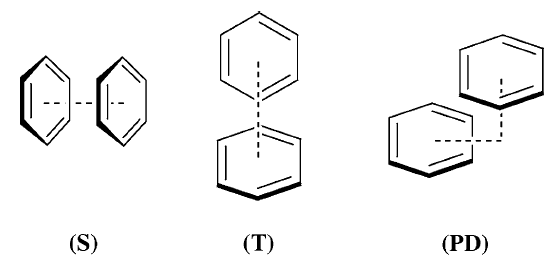
\includegraphics[scale=0.8]{image/Prot} \label{figprot}
   						\caption[Structures du dimère de Benzène]{Structures des dimères de Benzène : (S) Sandwich, (T) En forme de T et (PD) Parallèle Déplacé}
   					\end{figure}
   					
   					L’analyse de ces travaux montre que le débat pour estimer quelle est la conformation la plus stable est loin d’être clos. La majorité des travaux rapportent que ce sont les formes T et PD qui sont les plus stables. Pourtant, intuitivement il ne serait pas illogique de penser que la configuration en sandwich, qui correspond à la superposition maximal des deux monomères, puisse apparaitre comme suffisament stable du fait de la maximisation des interactions dispersives. La configuration parallèle déplacée est, quand à elle, souvent observée dans les expériences réalisées à l’état cristallin de composés purement aromatiques \cite{hunter1991pi,fyfe1997synthetic,rebek1996assembly} ou dans les études cherchant à caractériser les interactions des chaînes latérales aromatiques de protéines \cite{hunter1991pi,burley1985aromatic}.
   					Klemperer et al \cite{janda1975benzene} ont, quand à eux, rapportés que la configuration en T était prédominante à l’état gazeux. D’autres travaux issus de l’analyse des spectres rotationnel d'Arunan et Gutowsky \cite{arunan1993rotational}, en accord avec les études Raman de Henson et al \cite{henson1992raman} rapportent que les structures favorables du dimère du benzène s’approchent de la conformation T sans pour autant la confirmer.\\ 
   					
   					
   					Il existe dans la littérature une très grande variété d’approches concernant l’étude des dimères du benzène.
   					Nous faisons le choix de ne reporter, dans le tableau ci-dessous, que les modélisations conduisant aux résultats, à priori du fait des méthodes employées, les plus précis et qui font référence. Les travaux de Park et Lee \cite{park2006accurate}, de Tsuzuki et al \cite{tsuzuki2002origin} et de Sinnokrot et al \cite{hobza1996potential} ont tous été obtenus a partir de calculs CCSD(T) avec extrapolation CBS de base (en anglais Complete Basis Set extrapolation).
   					Cette méthodologie est une technique de calcul empirique basée sur un minimum de trois calculs séparés avec des bases de plus en plus complètes telles que les bases de type cc-pVXZ (X=T, Q, 5 …). 
   					Cette technique est une estimation approchée d’un résultat obtenu en utilisant une base infini. Elle permet d’atteindre la limite
   					de précision de la méthode de calcul la plus performante.
   					Nous avons reportés dans le tableau les résultats que nous avons obtenus sur la forme PD qui est celle qui à priori nous intéresse en priorité puisque c’est celle qui a été caractérisée expérimentalement à l’état solide (comme le seront les structures que nous aurons à modéliser dans notre travail issus des données IR obtenues en photo acoustiques). On peut remarquer, en accord avec toutes les données actuellement disponibles sur les approches SAPT, que notre valeur d’énergie d’interaction calculée en SAPT(PBE0)/aug-cc-pVTZ est totalement conforme à la valeur attendue. Sans surprise, l’approche SAPT
   					permet donc de reproduire avec une excellente vélocité les énergies d’interaction de systèmes en interaction pi-pi et d’atteindre la précision nécessaire pour reproduire des données aussi faibles que 1 à 2 kcal/mol. 
   					
   					
   					
   					\begin{table}[H]
   						\caption{Energie d'interaction du dimère de Benzène avec CCSD(T) en kcal/mol et DFT-SAPT (PBE0)}
   						\begin{center}
   							\begin{tabular}{l c c c c}
   								\toprule
   								& & T& & PD\\
   								\midrule
   								Park et Lee$^{1}$ & & -2,67& &-3,03\\
   								Tsuzuki et al$^{2}$ & & -2,46& & -2,48\\
   								Sinnokrot et al$^{3}$ & & -2,74& & -2,78\\
   								Hobza et al$^{4}$ & & -2,17& & -2,01\\
   								DFT-SAPT (PBE0) & & & & -2.35\\
   								\bottomrule
   							\end{tabular}
   						\end{center}
   						\centering
   						\footnotemark[1]{ref \cite{park2006accurate}},
   						\footnotemark[2]{ref \cite{tsuzuki2002origin}},
   						\footnotemark[3]{ref \cite{sinnokrot2002estimates}},
   						\footnotemark[4]{ref \cite{hobza1996potential}}
   						
   						[1] CCSD(T)/CBS
   						[2] CCSD(T)/CBS 
   						[3] CCSD(T)/CBS
   						[4] CCSD(T)/aug-cc-pVDZ
   						[5] SAPT(PBE0)/aug-cc-pVTZ
   						
   						
   						\label{benzene}
   					\end{table}
   					




%\newgeometry{textwidth=16cm}
\singlespacing
\chapter[Molecular dynamics study of the nano-aggregation in asphaltene]{Molecular dynamics study of the nano-aggregation in asphaltene mixtures: effects of the N, O and S heteroatoms}
\minitoc
\restoregeometry

\newpage


\textit{We present molecular dynamics simulations (MDS) for interpreting the molecular aggregation of:}
\begin{enumerate}
	\item \textit{six different asphaltene molecular models based on the C5Pe molecule;}
	\item \textit{several other derivatives based on the PA3 and CA22 structure issued from the recent work of isolation and identification of asphaltenes by Schuler \textit{et al.}\footnote{\textit{JACS}, \textbf{2015}, 137, 31, 9870}}
\end{enumerate}    

\textit{These simulations are based on recent X-ray (SAXS) and neutron (SANS) small-angle scattering experiments from Eyssautier \textit{et al.}\footnote{\textit{The J. of Phys. Chem. B}, \textbf{2011}, 115, 21, 6827} which proposed a discoidal asphaltene nanoaggregate structure of 0.67 nm height and its chemical composition. For the first topic, we have investigated the effect of sulfur atom position in the asphaltene structure and we have found that when it is grafted directly to the conjugated core no effect can be deducted from the stability of dimers and trimers and all the other studied parameters. This is not the case when sulfur is located in the lateral chain, where it has a particular affinity with oxygen and hydrogen atoms of the acid chain ends of neighbor molecules. Consequently, we suggest that these configurations of the sulfur atom are more likely to be problematic in oil industry. For the second topic, the chemical characteristics of these real asphaltene molecules were screened by changing the heteroatoms on the backbone and the lateral chain-ends. The results show that the interaction energies vary for different heteroatom arrangement within a given structure and depend on the type of asphaltene. Moreover, we showed that the chain-ends have a crucial role on this phenomenon.}

\clearpage

\section{Introduction}

%%%%%%%%%%%%%%%%%%%%%%%%%%%%%%%%%%%%%%%%%%%%%%
%     À VOIR SI ÇA VAUT LA PEINE D'INCLURE CE MORCEAU CI-DESSOUS      %
%%%%%%%%%%%%%%%%%%%%%%%%%%%%%%%%%%%%%%%%%%%%%%

Asphaltenes are the oil's insoluble phase in light \textit{n}-alkanes and soluble in aromatic solvents like benzene or toluene\cite{mullins2011asphaltenes}. Their presence is critical and can cause problems in several fields of petroleum utilization, from oil recovery and transportation to refining.\cite{adams2014asphaltene} These complications arise from the tendency of asphaltenes to aggregate and form macro structures able to modify their flow properties (increasing oil viscosity, emulsion stability, etc.) and even, in the worst cases, stop the fluid production (plugging pores in the reservoir, well-bore tubing or flow-lines/pipelines, accumulating in separators, etc.) \cite{benamsili2013multi}.\\

Asphaltenes consist of a complex mixture of polycyclic aromatic hydrocarbons substituted with alkyl side chains. Carbon and hydrogen are the major atoms, but the molecules also contain heteroatoms, mainly sulfur.\cite{mullins2010modified} Although much knowledge has been gained throughout the last years, the molecular structure of this phase is poorly determined and can vary quite significantly depending on the origin, on the age of the crude oil and on the pressure and temperature conditions\cite{sabbah2011evidence}.\\

So, in order to fully understand their nature and to predict their structure, several analytical techniques have been used to gather information on their macromolecular structure. Small angle X-ray (SAXS) and neutron scattering (SANS) techniques have proved that the basics of their supramolecular arrangement is the discoidal $\pi$-stacking of the conjugated cores, with heights varying from 1 to 10 nm \cite{eyssautier2011insight,barre2009relation}.\\

From \textit{in silico} point of view, the study of asphaltene aggregation makes use of molecular dynamics simulations. Several force-fields have proved to produce results consistent with experimental results.\cite{sedghi2013effect,liu2015molecular,gao2014molecular} Thereby, we have, in a first moment, chosen six asphaltene molecular models, as dimers and trimers in toluene, to investigate the sulfur atom position in the structure and the consequent effect on the stability of dimers and trimers in solution. These models are based on the C5Pe model module, a prototypical asphaltene molecule that has been reported and used in several studies\cite{gao2014molecular,teklebrhan2014initial}.\\

Experimental work in progress using this molecule also justifies this choice that allows us to compare experience and theory. This work aims to investigate the influence of sulfur atoms on C5Pe's dimers and trimers stabilization during a 150 ns time-delay in toluene at 298K and 1 atm conditions. In this way, all the other possible parameters influencing the nano-aggregation of asphaltenes (size of conjugated core, lateral chains, etc...) are excluded and one can really screen the effect of sulfur atoms in this physical-chemical process.\\

Then, the first part of this study uses the N-(1-Hexylheptyl)-N'-(5-carboxy-licpentyl)-perylene-3,4,9,10-tetracarboxylicbisimide molecule (C5Pe, molecule 1) and three C5Pe analogues (molecules 2, 3, and 4), with the presence of sulfur atom at different positions (core and side chain) as test cases. Two other molecules, 5 and 6, respectively, were studied: the situation where all the \ce{C=O} groups are replaced by \ce{C=S} ones (the extreme of molecule 2) and the situation where no heteroatom is found in this position (\ce{C-H} bond, quinoid structure imposed). 

\begin{figure}[htb]
	\centering
	\begin{tabular}{cc}
		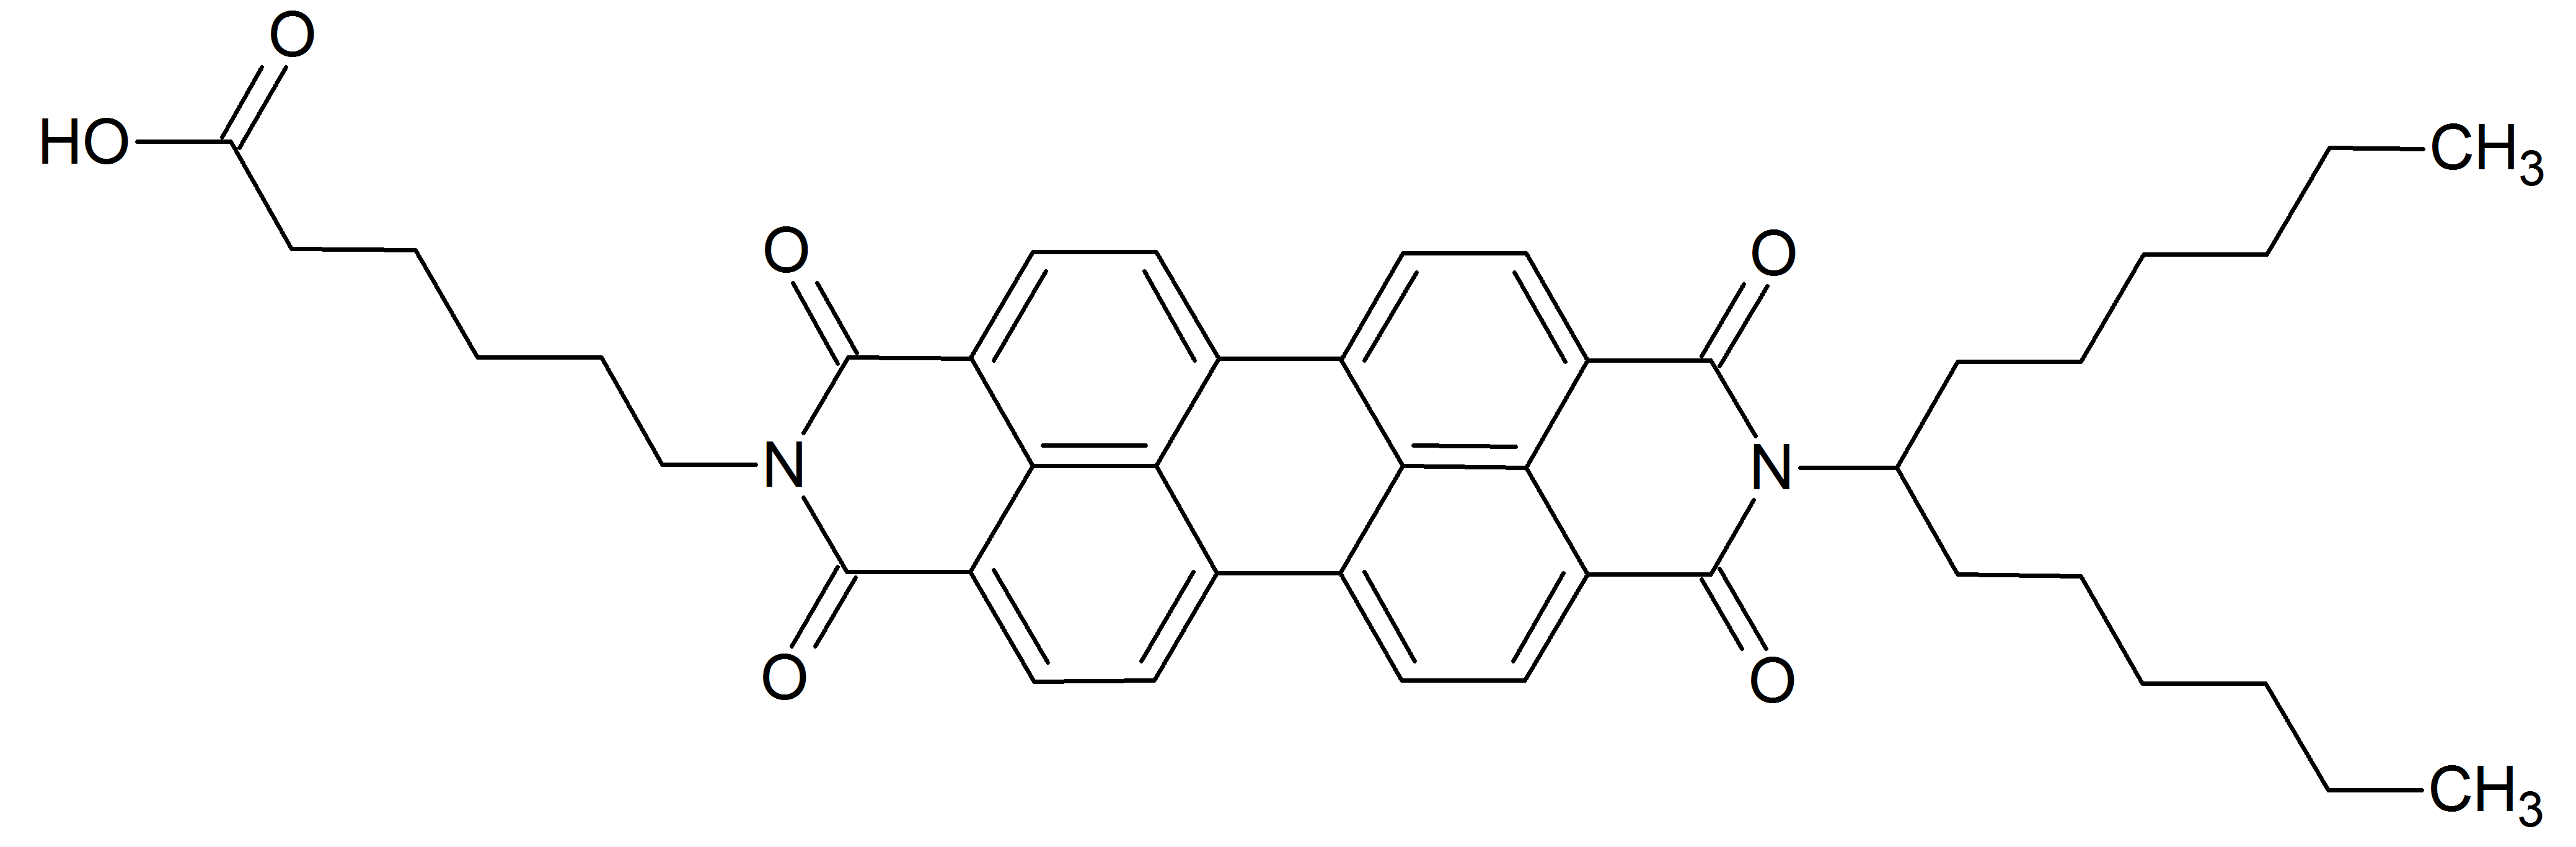
\includegraphics[width=0.45\columnwidth]{image/1} &
		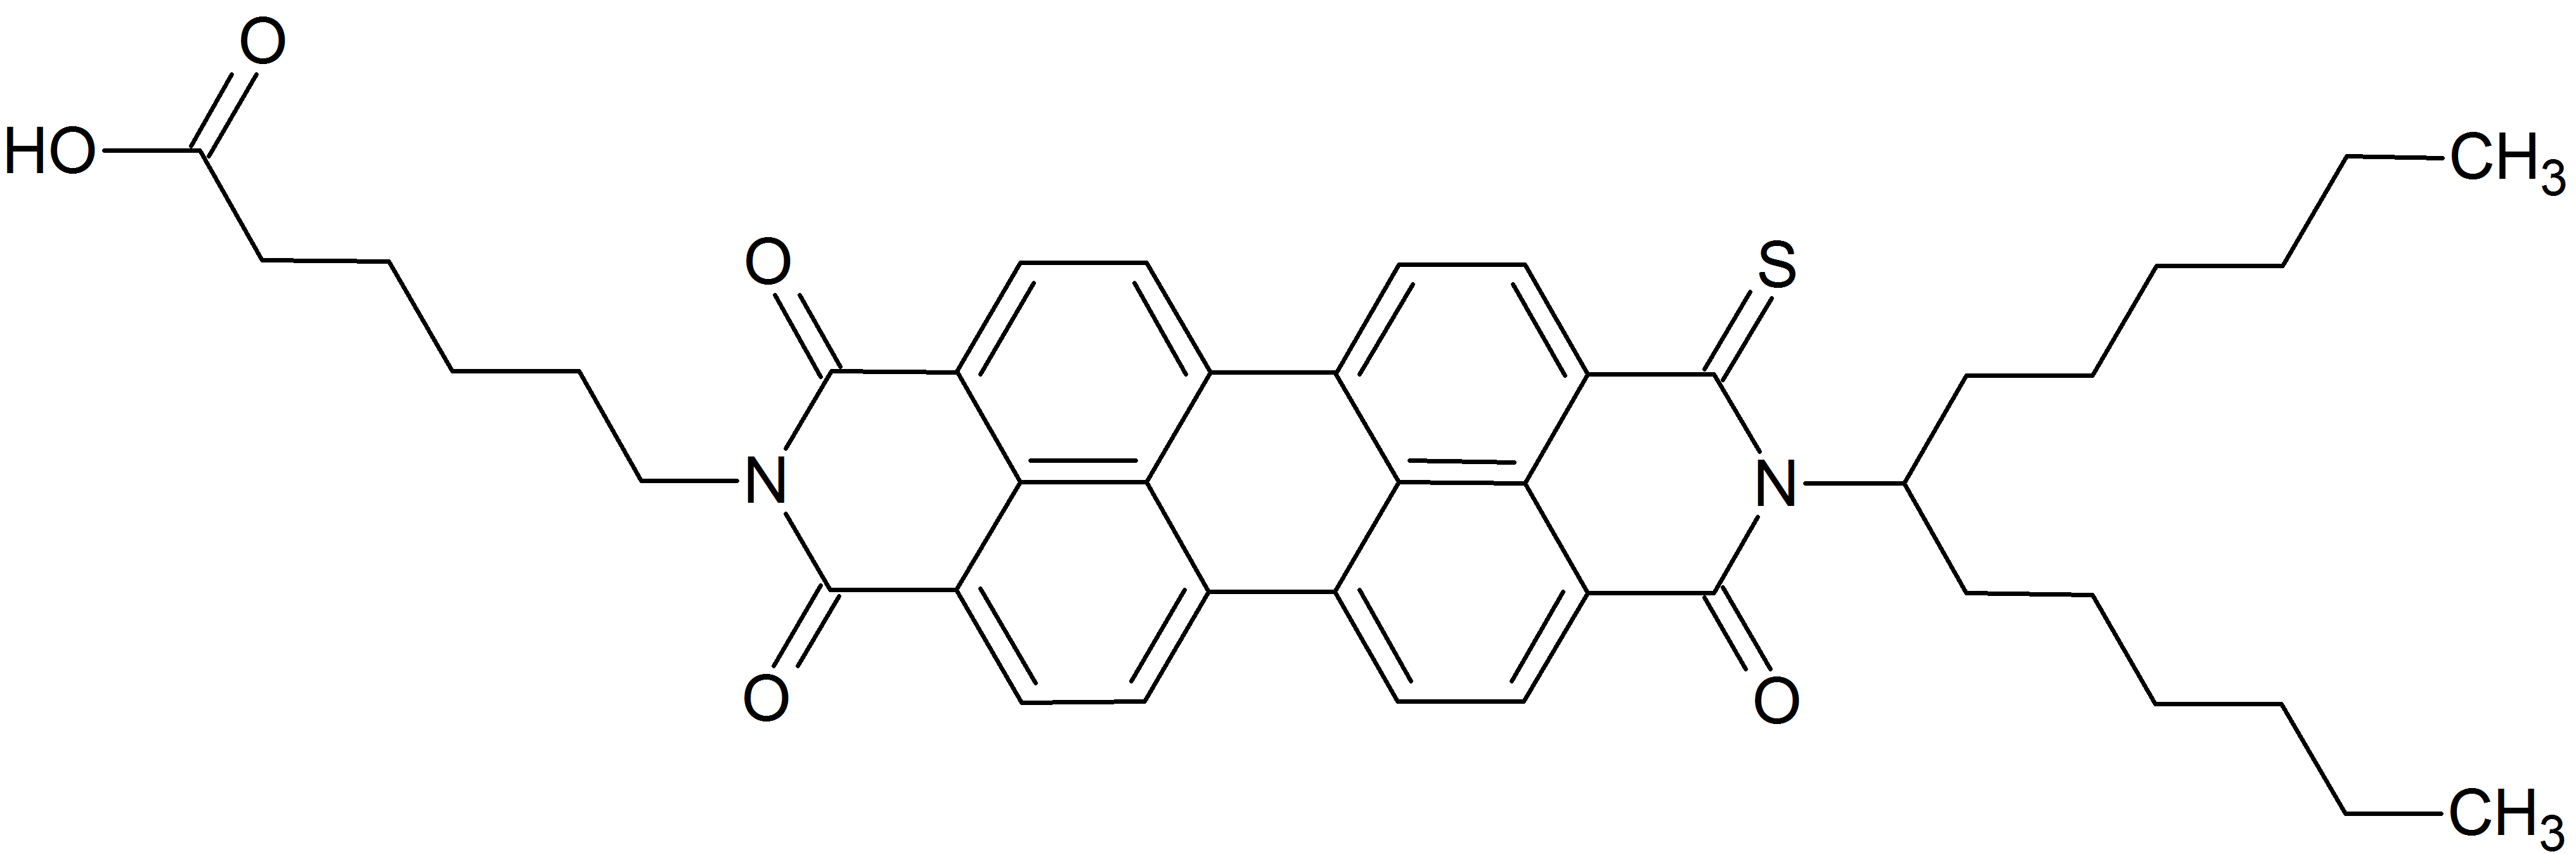
\includegraphics[width=0.45\columnwidth]{image/2}\\
		Molecule 1 & Molecule 2\\
		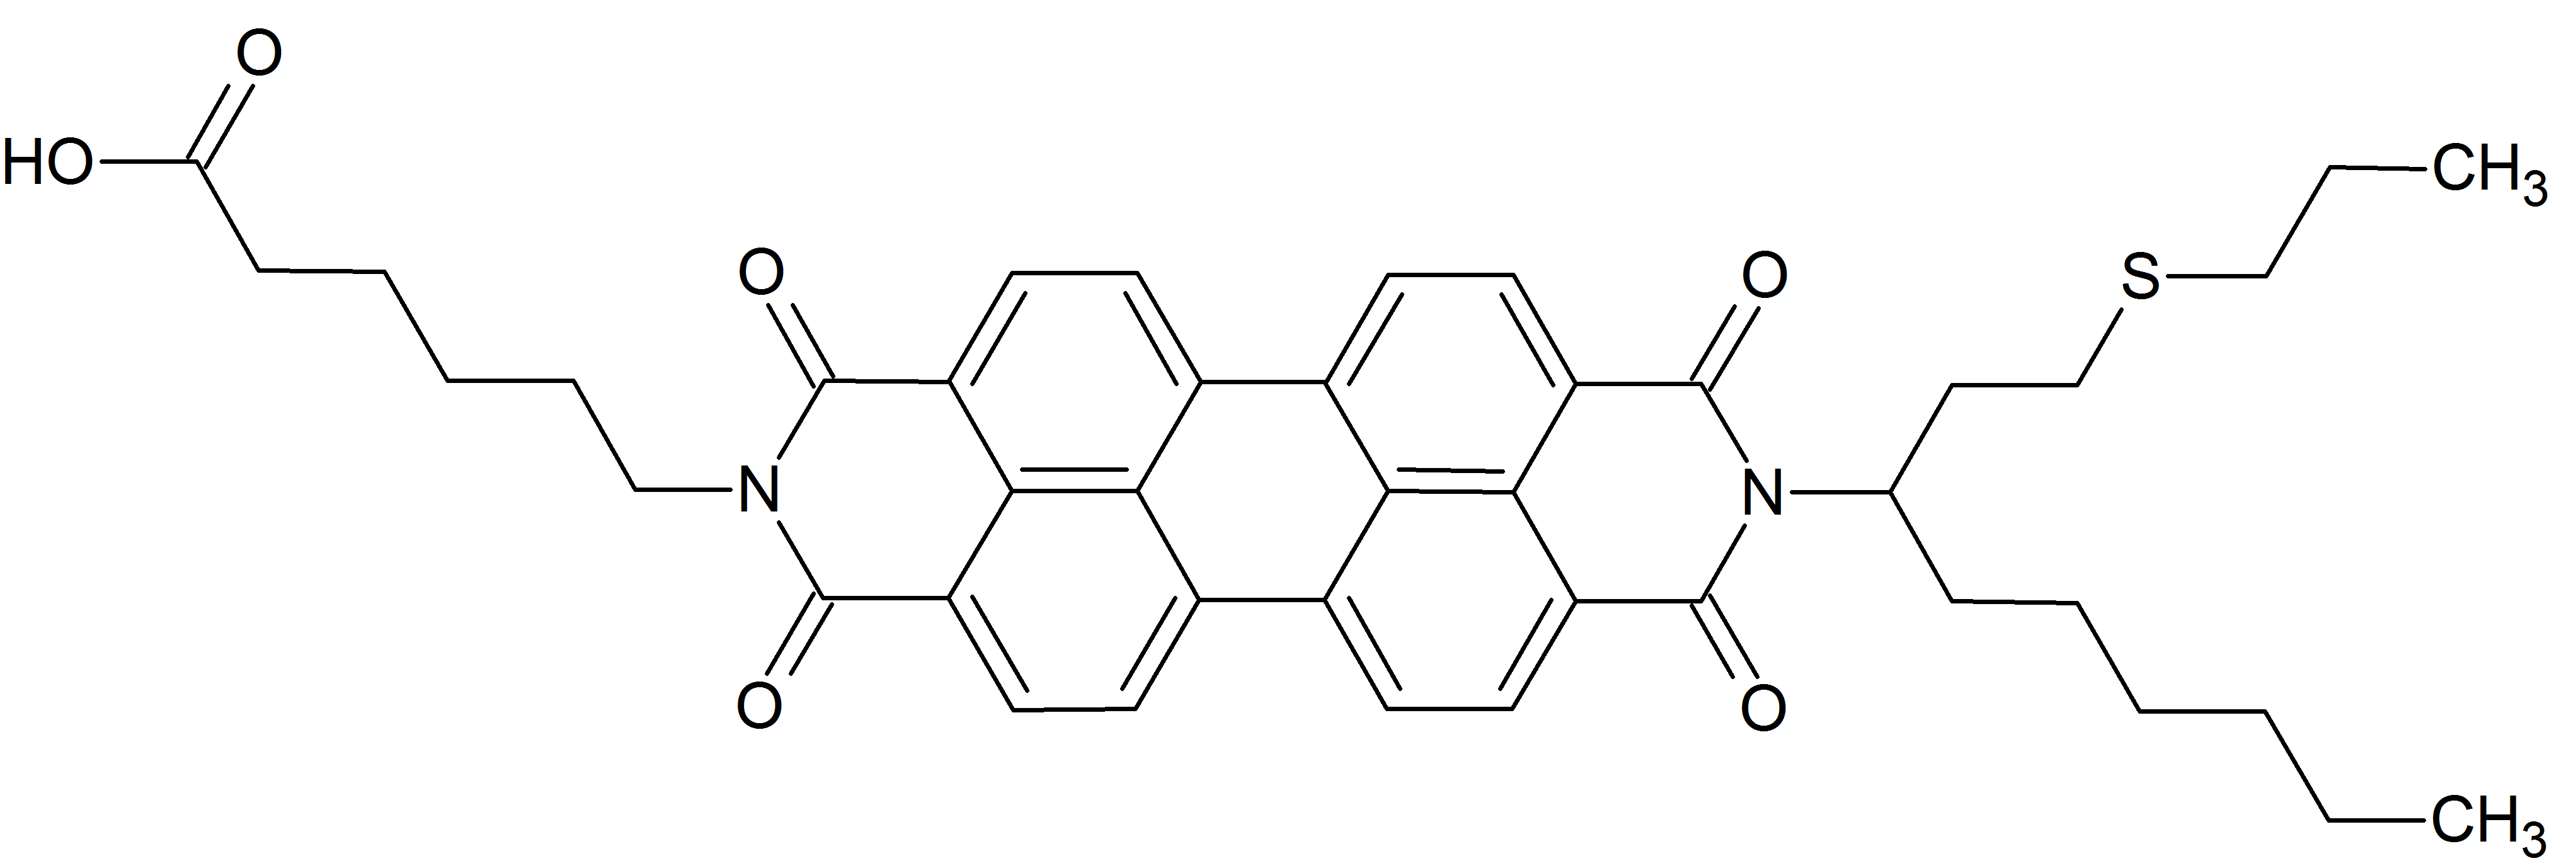
\includegraphics[width=0.45\columnwidth]{image/3} &
		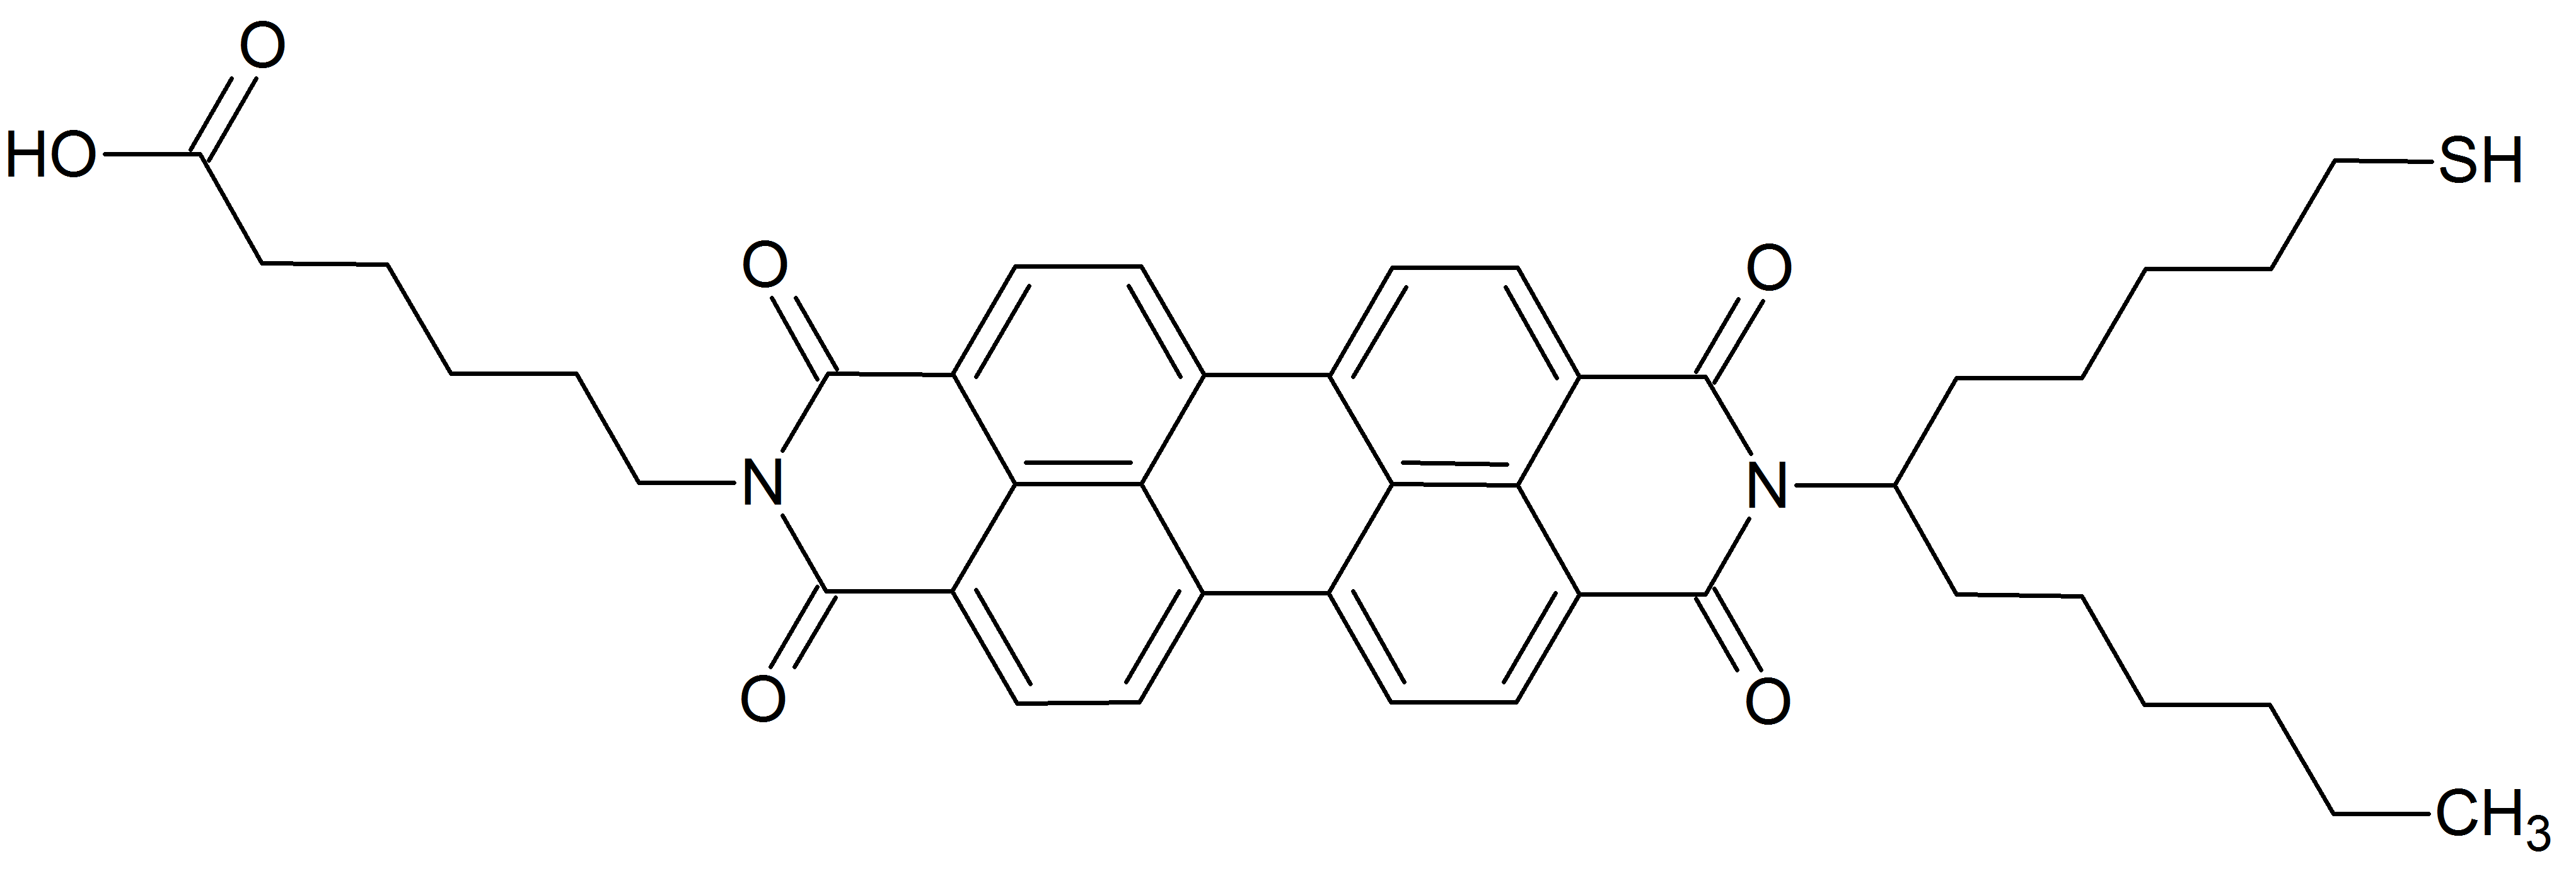
\includegraphics[width=0.45\columnwidth]{image/4}\\
		Molecule 3 & Molecule 4\\
		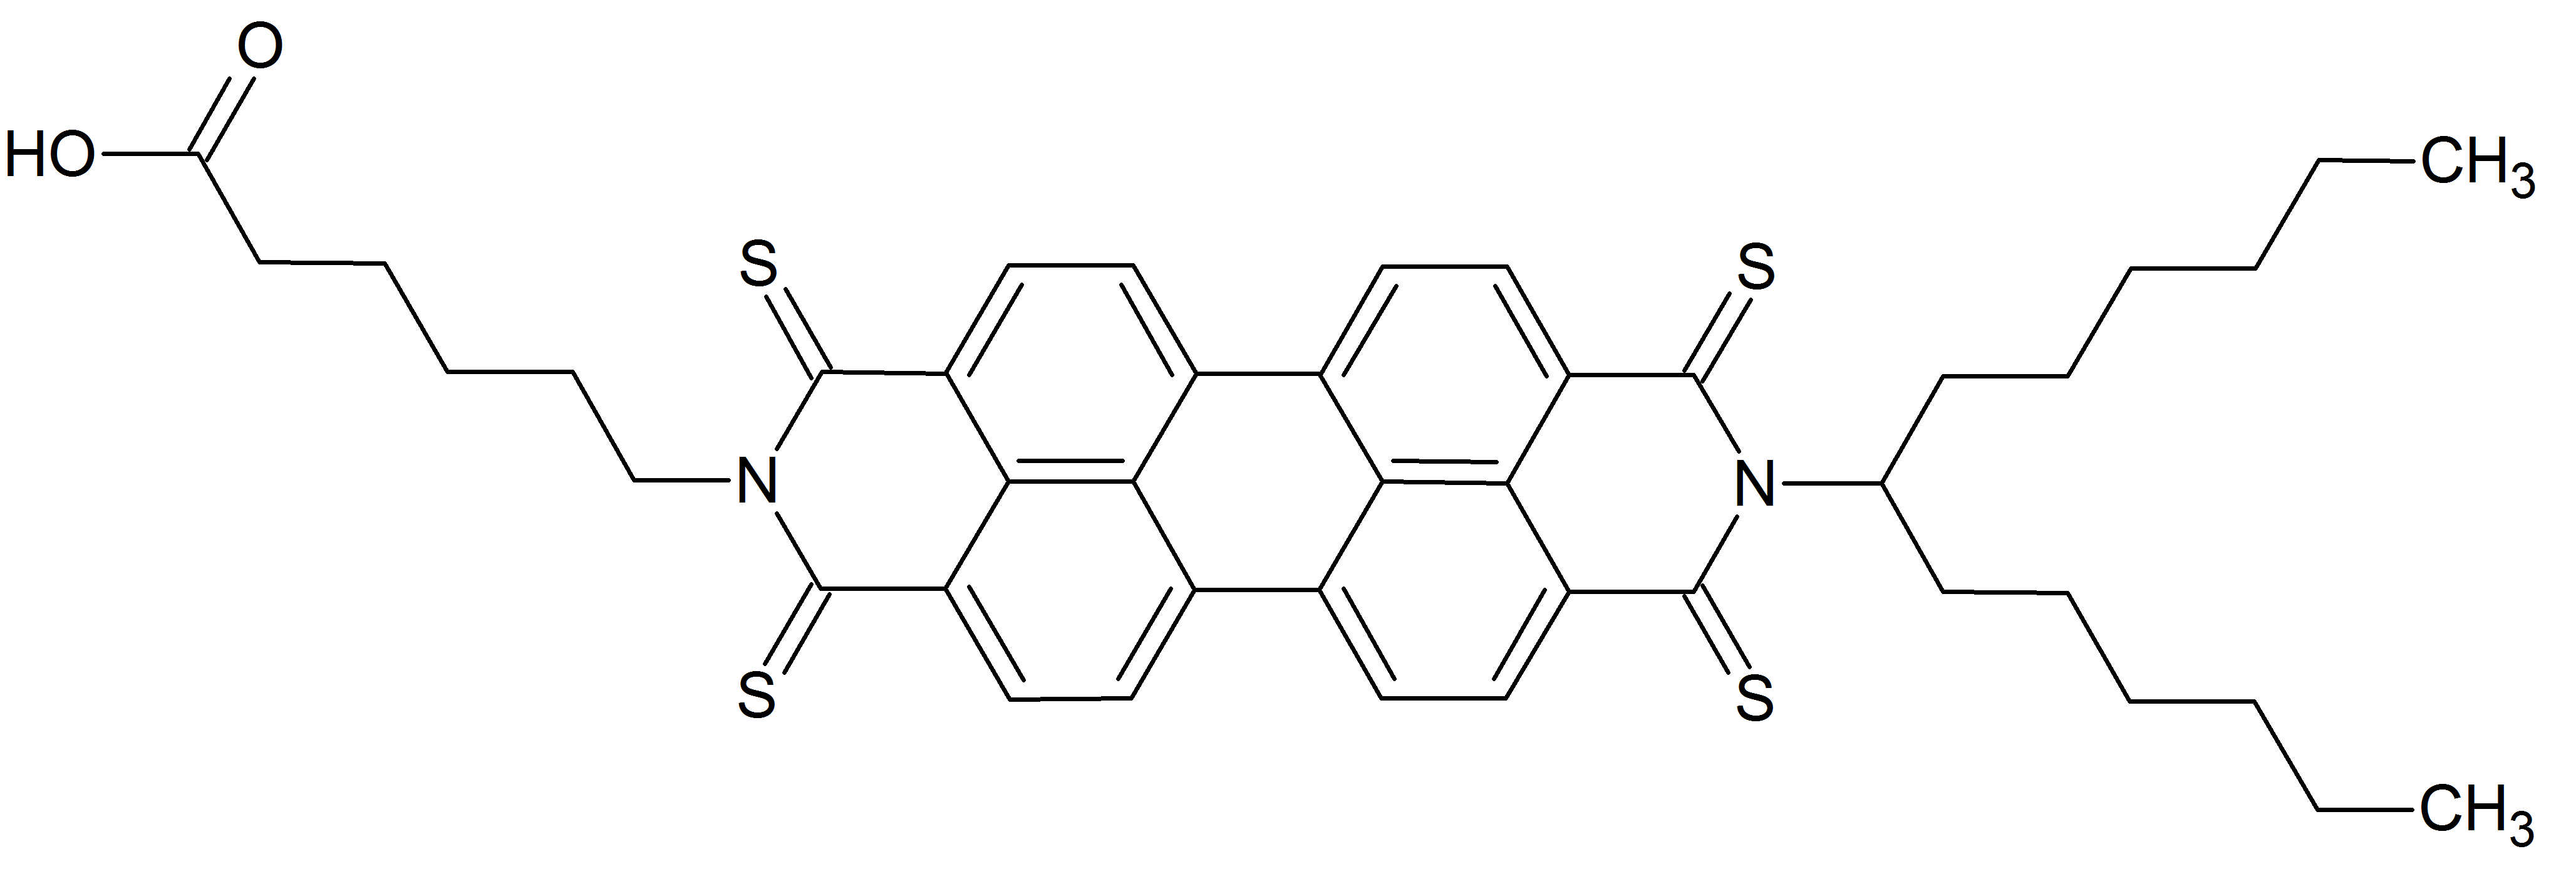
\includegraphics[width=0.45\columnwidth]{image/5} &
		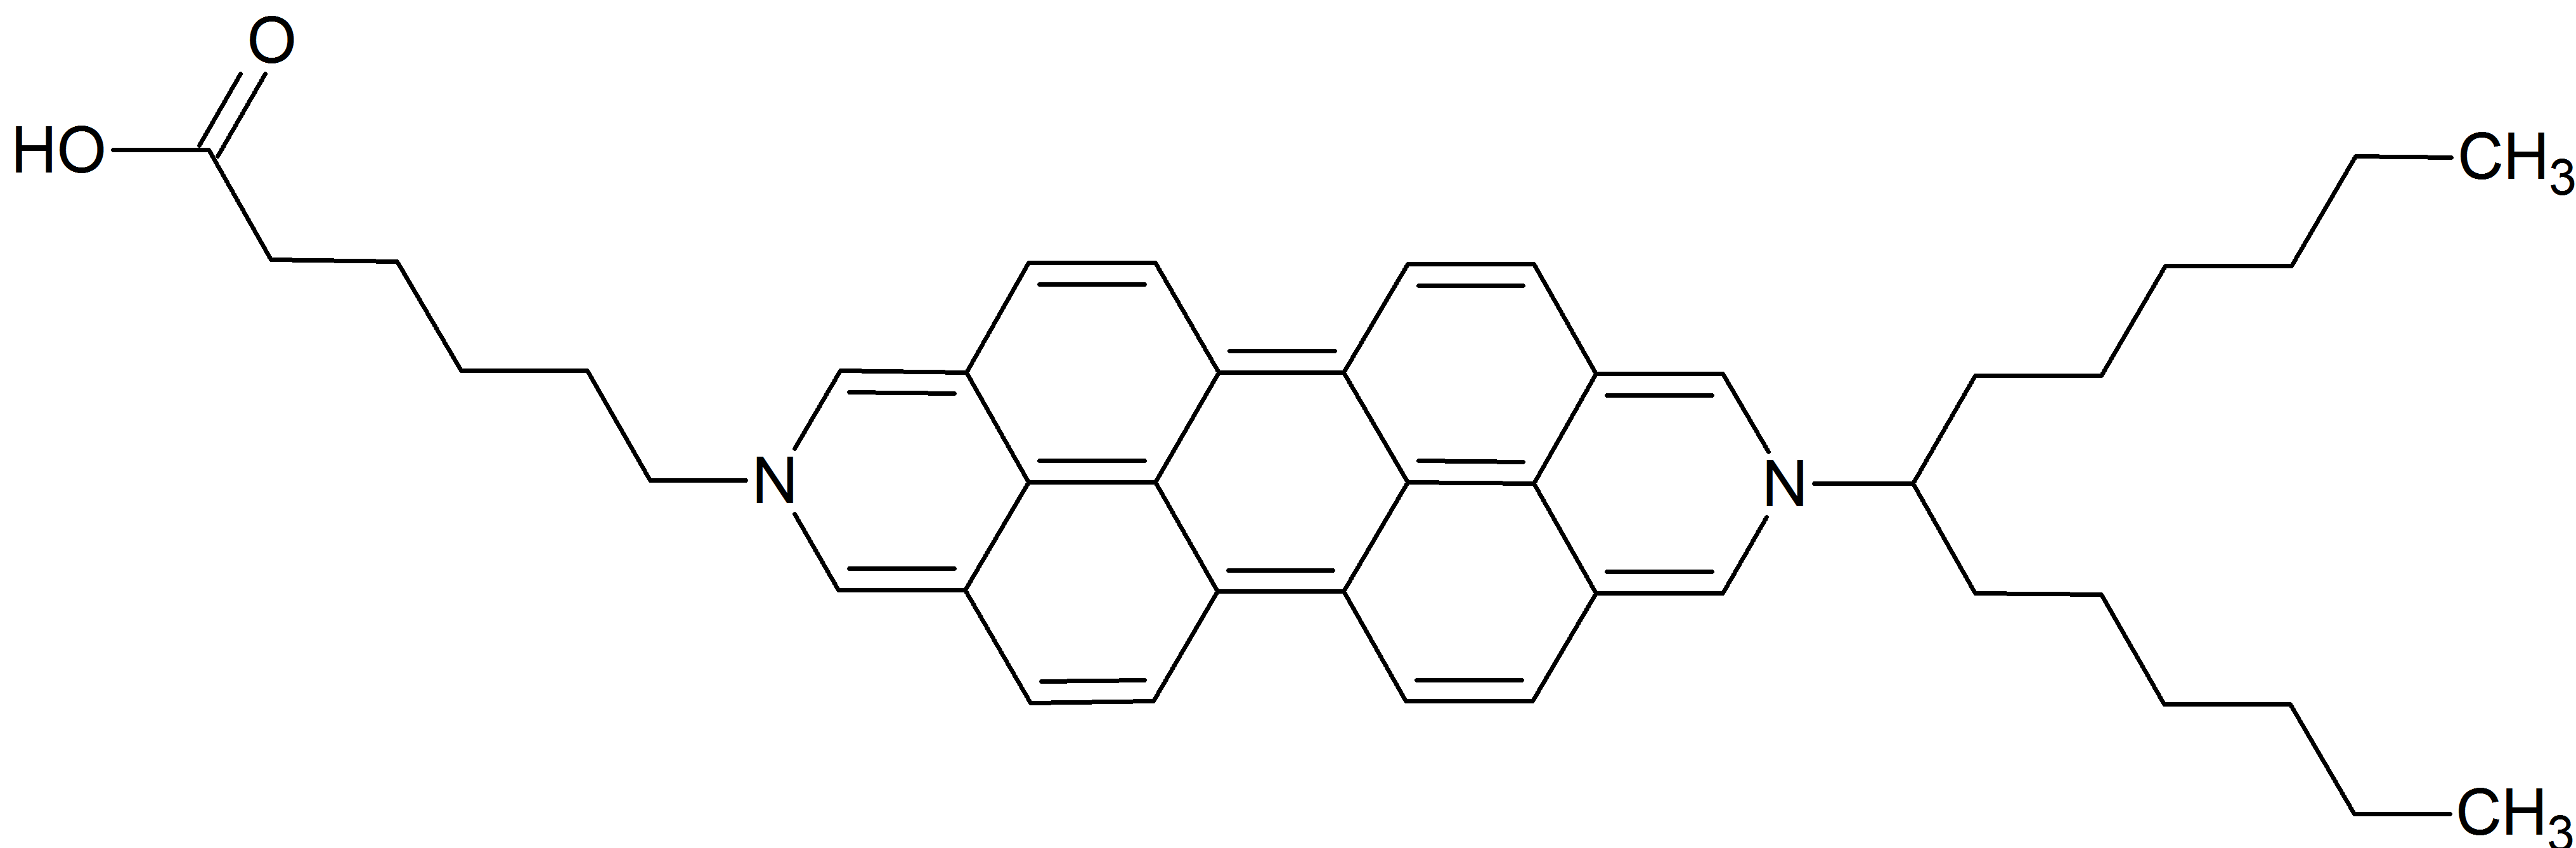
\includegraphics[width=0.45\columnwidth]{image/6}\\
		Molecule 5 & Molecule 6\\        
	\end{tabular}
	\caption{C5Pe molecular models of asphaltenes. }
	\label{pap:fig01}
\end{figure}

For each solvated asphaltene system using the C5Pe model, the initial configuration was constructed in a box with the 2 or 3 asphaltene molecules models. Two starting points were envisaged: 1) their poly-aromatic cores are anti-parallel to each other and the aggregate is already formed (this is called the``organized'' configuration); and 2), the molecules were randomly inserted in the simulation box. For the former case, the spacing between the mass centers of two neighboring asphaltene molecules is 0.35 nm in the -stacking direction. Finally, for both cases, the box was randomly filled with toluene molecules.\\

More recently, Schuler \textit{et al.}'s\cite{schuler2015unraveling} work brought more evidences on the molecular structures of asphaltenes based on Atomic Force Microscopy (AFM). They report the isolation of several distinct molecules which are in good agreement with the commonly accepted asphaltene structure: basically composed of aromatic cores, substituted by heteroatoms and presence of alkyl side chains with a variable number of carbons. We have chosen two among these molecules in order to study the effect of the heteroatom substitution on the conjugated aromatic core and the mixture in the crude oil and how the aggregation can occur in a more realistic model than just using one molecule at a time. The selected molecules, depicted in Figure \ref{pap:fig01}, are originally labeled PA3 and CA22 after Schuler \textit{et al.},\cite{schuler2015unraveling} both of them being of the continental type.\cite{mullins2010modified,mullins2011asphaltenes,mullins2012advances} Finally, it is worth saying that the CA22 molecule is a coal asphaltene rather than a petroleum asphaltene. It is herein used since it has a conjugated core size sensibly different from the PA3 one.

\begin{figure}[htb]
	\centering
	\begin{tabular}{cc}
		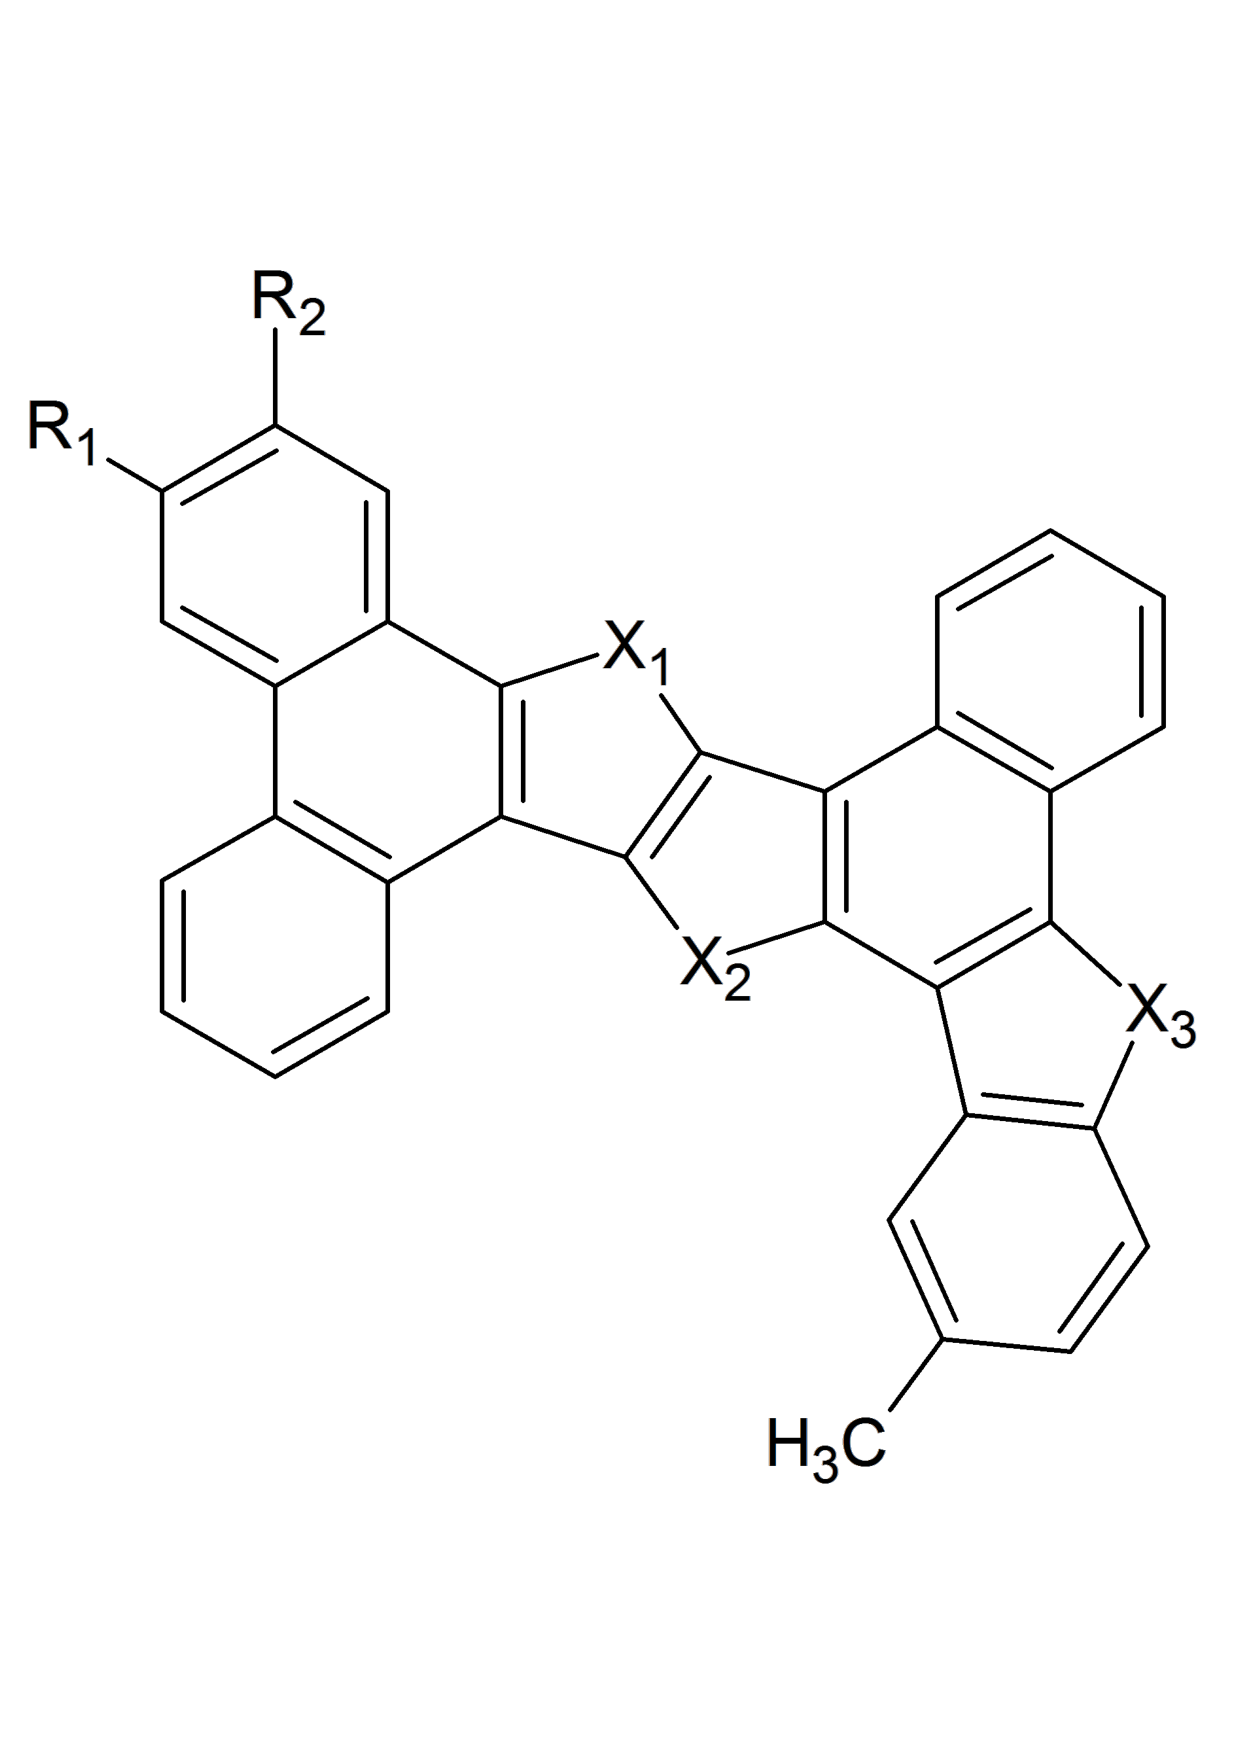
\includegraphics[width=0.35\columnwidth]{image/PA3} &
		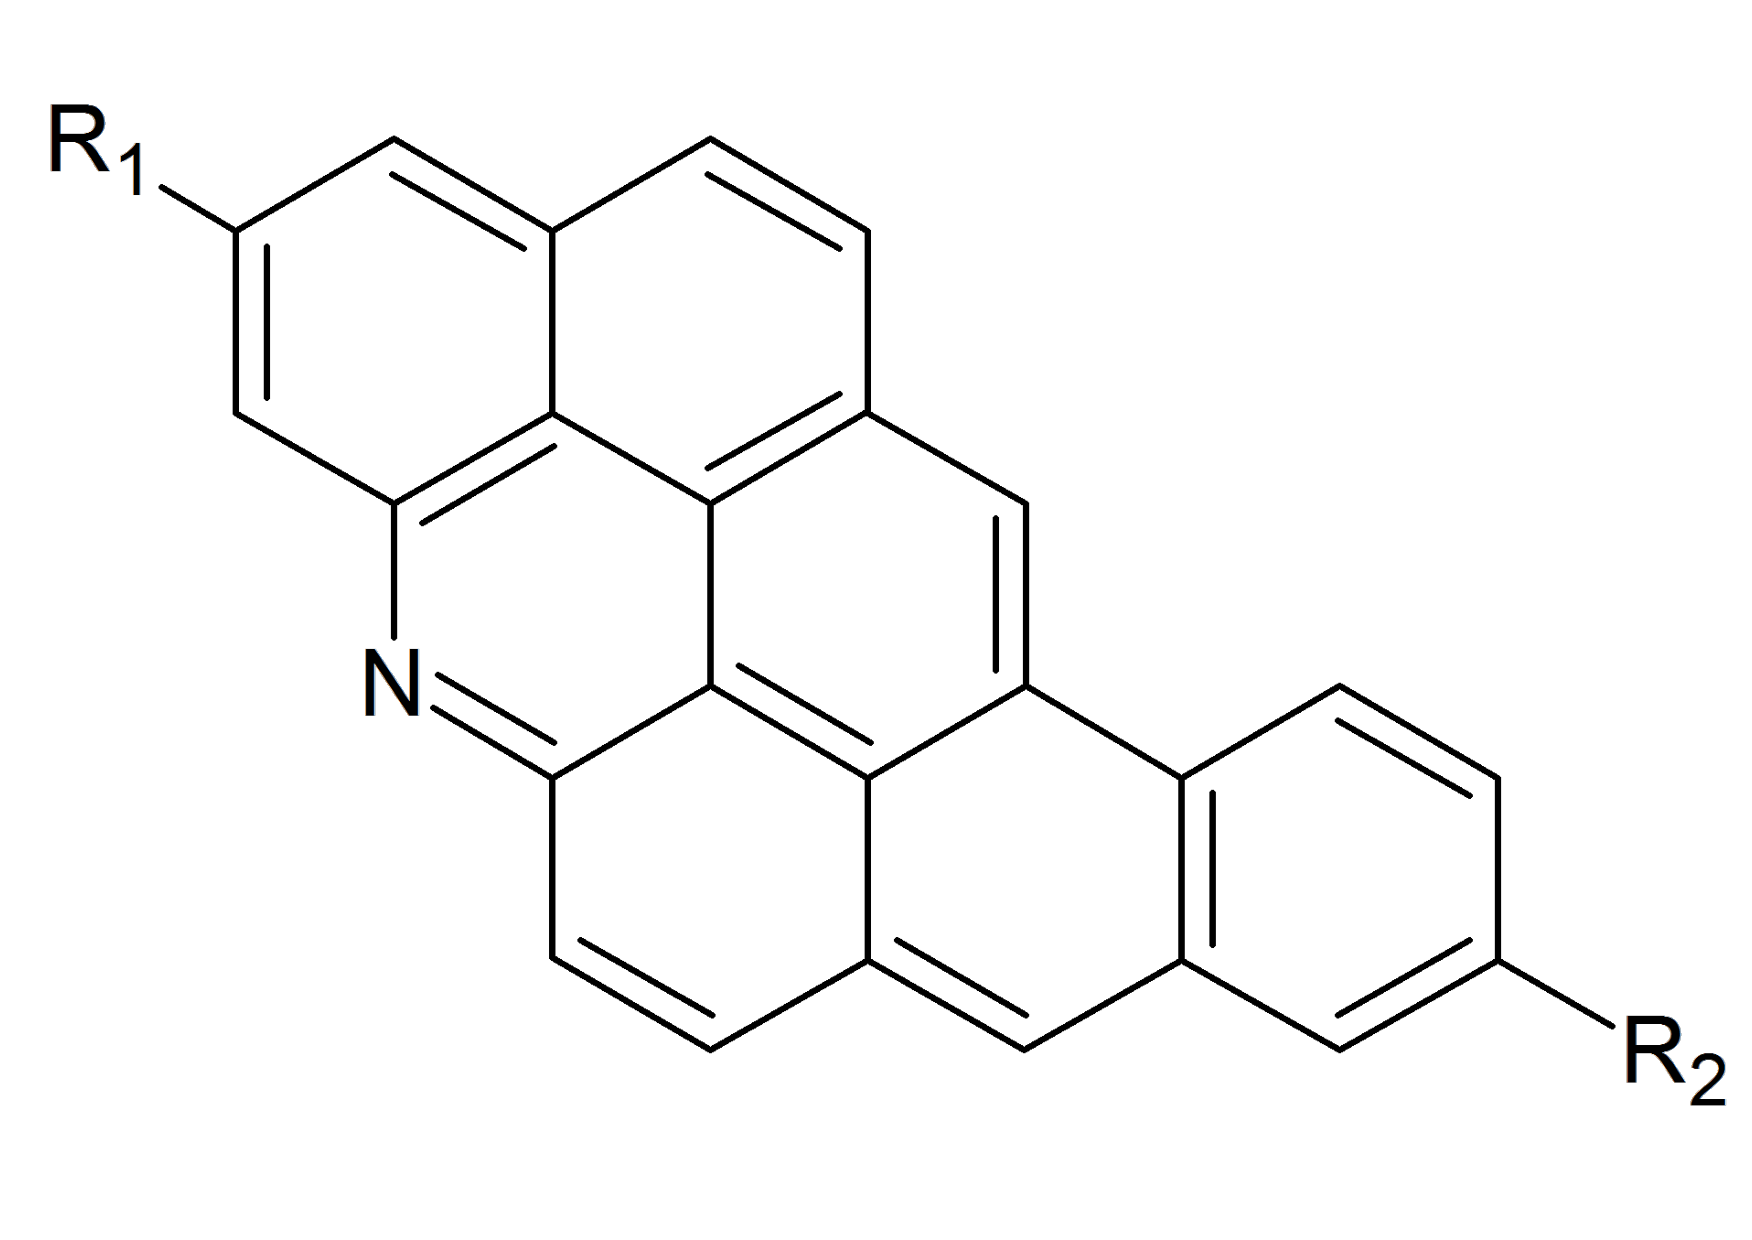
\includegraphics[width=0.35\columnwidth]{image/CA22}\\
		(a) & (b)\\
	\end{tabular}
	\caption{Two different asphaltene structures found in the crude petroleum: (a) PA3 and (b) CA22. $R_1$ and $R_2$ are the $n$-hexyl lateral chains which can have \ce{-COOH} or \ce{-CH3} as chain-ends. $X_n$ (n=1-3) can be \ce{O}, \ce{S}, or \ce{NH} atom groups.}
	\label{pap:fig02}
\end{figure}

These molecules had their lateral chain-end varied as well as the heteroatom on their conjugated cores. This allowed us to have 14 different molecular structures that were studied separately and together in different proportions. In this way, the aim of this paper is to study the first steps of the asphaltene nano-aggregation by molecular dynamics simulations (MD) as a function of their chemical composition. For PA3, the choice of the heteroatom was motivated by previous  Fourier transform ion cyclotron resonance mass spectroscopy (FT-ICR-MS) results indicating their presence in the aromatic core.\cite{kim2009automated,stanford2007compositional} In the case of CA22, nitrogen was chosen because of the relatively high stability of 6-atoms cycle compared to what can be obtained using the other heteroatoms. These molecules were declined following the tabulation in Table \ref{pap:tab01}. They are classified following their number of carbon atoms (NbC), their Double Bond Equivalent (DBE) and the Class to which they belong accordingly to FT-ICR-MS, \cite{kendrick1963mass,hughey2001kendrick,shi2010characterization} which indexes might be of use for further referring.

\begin{table}[htb]
	\caption{Labelling of the systems used in this study, with the chain-ends of the lateral chains. Molecules A11-A53 are of the type PA3 and AAA, AAB and AAC are of the type CA22. NbC is the number of Carbon atoms of the structure, DBE is the Double Bond Equivalent and Class stands for the nomenclature reporting the number of heteroatoms found in the structure by FT-ICR-MS. $M_w$ is the molecular weight of each molecule.}
	\centering    
	\begin{tabular}{c|ccc|cc|ccc|c}
		\hline 		
		\textbf{Label} & $X_1$ & $X_2$ & $X_3$ & $R_1$ & $R_2$ & NbC & DBE & Class & $M_w$ (g.mol$^{-1}$)  \\
		\hline 
		\textbf{A11} & O & O & O & \ce{COOH} & \ce{COOH} & 45 & 27 & \ce{O7} & 690.8\\
		\textbf{A12} & O & O & O & \ce{CH3} & \ce{COOH} & 45 & 26 & \ce{O5} & 660.8\\
		\textbf{A13} & O & O & O & \ce{CH3} & \ce{CH3} & 45 & 25 & \ce{O3} & 630.8\\
		\textbf{A21} & S & S & S & \ce{COOH} & \ce{COOH} & 45 & 27 & \ce{S3O4} & 740.0\\
		\textbf{A23} & S & S & S & \ce{CH3}& \ce{CH3} & 45 & 25 & \ce{S3} & 679.0 \\
		\textbf{A31} & NH & NH & NH & \ce{COOH} & \ce{COOH} & 45 & 27 & \ce{N3O4} & 687.8 \\
		\textbf{A33} & NH & NH & NH & \ce{CH3} & \ce{CH3} & 45 & 25 & \ce{N3} & 627.8\\
		\textbf{A41} & O & O & S & \ce{COOH} & \ce{COOH} & 45 & 27 & \ce{O6S} & 706.8\\
		\textbf{A43} & O & O & S & \ce{CH3} & \ce{CH3} & 45 & 25 & \ce{O2S} & 646.8 \\
		\textbf{A51} & O & S & S & \ce{COOH} & \ce{COOH} & 45 & 27 & \ce{O5S2} & 723.9\\
		\textbf{A53} & O & S & S & \ce{CH3}& \ce{CH3} & 45 & 25 & \ce{OS2}& 662.9 \\
		\hline
		\textbf{AAA} & - & - & - & \ce{COOH} & \ce{COOH} & 37 & 22 & \ce{N1O4} & 555.6\\
		\textbf{AAB} & - & - & - & \ce{COOH} & \ce{CH3} & 37 & 21 & \ce{N1O2}&525.7 \\
		\textbf{AAC} & - & - & - & \ce{CH3} & \ce{CH3} & 37 & 20 & \ce{N1} & 501.7\\
		\hline
	\end{tabular}
	\label{pap:tab01}
\end{table}

The DBE in this table was calculated as:

\begin{equation}
DBE = C - \frac{H}{2} + \frac{N}{2} +1
\end{equation}

Where C, H and N stand respectively for the number of carbon, hydrogen and nitrogen atoms. The labeling system relies on the following logics: the first ``A'' stands for ``asphaltene'', the second character identifies a different family of molecules: numeric for each type of different molecule within the PA3 family and alphabetic for each type of different molecule within CA22 family. The last character identifies the number of acid chain ends: index 1 for two acid chain ends \ce{-COOH}, index 2 for one acid chain \ce{-COOH} end and one \ce{-CH3} and index 3 for two \ce{-CH3} chain ends (no acid).

For this ensemble of molecules, three distinct scenarios were studied:

\begin{enumerate}
	\item homogeneous boxes - boxes where each asphaltene molecule interacts with its equal;
	\item heterogeneous boxes - boxes where asphaltenes of the same class (PA3 or CA22) are studied among them;
	\item  \textit{super}-heteregenous boxes - boxes where at least one asphaltene molecule is of type PA3 and at least one is of type CA22; 
\end{enumerate}

This variation allowed us to span a large variety of mixing scenarios and to separate the different contributions of each physical-chemical factor having a role on the aggregation of asphaltenes. Finally, it is worthy saying that this work is a follow-up of the one recently published by our group,\cite{sodero2016investigation} in which we have studied the influence of the heteroatom position in a model asphaltene molecule.

However, all the studies available in literature very often take into account the presence of only one type of asphaltene at a time. This approach is not completely representative of the real very complex mixture that is the crude oil and the effect of rationally changing the chemical structure on the aggregation behavior of asphaltenes has, up to our knowledge, never been reported. Some authors have indeed studied the presence of different asphaltenes in the same simulation box but their interest was, mainly, the distribution of each type of molecules across the oil-water interface.\cite{frigerio2011multiscale,mikami2013molecular,yang2015asphaltene}

\section{Simulation Method}

The MD simulations were carried out using the GROMACS 5.1.1 software package.\cite{berendsen1995gromacs,hess2008gromacs,van2005gromacs} The GROMOS96 force field\cite{van1998gromos} with the 53a6 parameter set\cite{oostenbrink2004biomolecular} was used in all calculations. This force field has already been tested on poly-aromatic molecules and has shown to be very useful in the dynamics of this type of system.\cite{teklebrhan2014initial,kuznicki2008molecular,kuznicki2009aggregation,teklebrhan2012probing}

Toluene was used as solvent in order to mimic the infinite dissolution effect and to avoid the formation of the aggregates due to polarity difference. The initial coordinates were used as input to the PRODRG 2.5 server\cite{schuettelkopf2004prodrg} to generate the GROMACS molecular topology and structure files. The topology of toluene molecule was generated from phenylalanine amino acid fraction in GROMACS. This method proved to be precise since it yields a calculated toluene density value of 0.88 g.cm$^{-3}$, in good agreement with the 0.86 g/cm$^{-3}$ value extracted from NIST WebBook (National Institute of Standards and Technology).\cite{nist}

The resulting topologies had their atomic charges adjusted in order to better reproduce the ones obtained by molecular quantum- mechanics methods, such as Density Functional Theory (DFT). 

The C5Pe derivatives had all partial charges for the compounds were used in the topologies based on the GROMOS96 force field parameters. For C=S group, the charges were applied as described by Huang and co-workers.\cite{huang2012molecular} For the molecules based on Schuler \textit{et al.}'s work, the Mulliken charges of the heteroatoms and their surroundings were obtained at the B3LYP/def2-SVP level of theory \cite{becke1993density,lee1988development,stephens1994ab,schafer1992fully,weigend2005balanced} using Orca 3.0.3 software\cite{neese2012orca}.\\

The first part of this study was divided into the study of dimers and trimers; separately, at a fixed concentration. For dimers, cubic boxes of 50 x  50 x 50 \AA~ were either filled randomly with the C5Pe-derivative molecules (random configuration) or filled with two molecules having their poly-aromatic cores are anti-parallel to each other and the aggregate is already formed (this is called the``organized'' configuration), as already mentioned. For the latter case, the spacing between the mass centers of two neighboring asphaltene molecules is 0.35 nm in the -stacking direction. Finally, for both cases, the box was randomly filled with toluene molecules. For trimers, so that the concentration could be kept constant, the simulation boxes now had 50 x  75 x 50 \AA~dimensions. The second part of this study, using the molecules reported by Schuler \textit{et al.}, a cubic box of 50 x  50 x 50 \AA~was randomly filled with 5 molecules of asphaltene and the solvent was then randomly added, as well.\\

Once the several distinct configurations of starting geometries were prepared, their energy was minimized by the steepest descent and conjugated gradients methods. Then, the systems were equilibrated in the NPT ensemble at 298 K and 1 bar pressure during 3 ns using the V-rescale thermostat\cite{bussi2007canonical}\footnote{For the systems using the C5Pe derivatives, the Berendsen thermostat was used for convenience reasons and this has no impact on the results of the calculations.} and Berendsen barostat.\cite{berendsen1984molecular} The production phase consisted of 60 ns of dynamics\footnote{150 ns for the C5Pe derivatives systems.} at 298 K  and 1 bar of pressure also under the NPT ensemble but using the Nosé-Hoover thermostat\cite{hoover1985canonical,nose1984molecular} and the Parrinello-Rahman\cite{parrinello1981polymorphic} pressure coupling algorithm. The initial atomic velocities were set using the Maxwell-Boltzmann distribution of the specified temperature. Throughout minimization, stabilization and production phases, a cutoff of 12 \textup{\AA} was used for both Coulomb and Van der Waals interactions. Periodic boundary conditions were thoroughly applied in the three directions. The Verlet integration algorithm\cite{verlet1967computer} has been used with a 2 fs integration step. The electrostatic interactions were computed using the Particle-Mesh Ewald\cite{essmann1995smooth} summation method with a fast Fourier transform grid spacing of 1.6 \textup{\AA}  to account for long-range electrostatic interactions of the system.  All the bond lengths have been constrained using the LINCS algorithm\cite{hess1997lincs} and this is based on the fact that the bond vibration periods are orders of magnitude quicker than the aggregation process. The neighbor list within 12 \textup{\AA} radius was updated every 5 steps.\\

After minimization, equilibration and production phases, each system was analyzed by calculating the radial distribution function (RDF). These functions are calculated considering the distribution of the distances between the center of mass of the selected residues. In our case, the asphaltene residue is consisted of the aromatic core and the lateral chain. In order to exclude the self-interaction (intra-molecular) configuration, the RDFs were calculated within the interval comprised between 2 and 25 \textup{\AA}. Moreover, the geometry of the poly-aromatic cores was also quantified by the cosine of angle between the poly-aromatic planes. 

%%%%%%%%%%%%%%%%%%%%%%%%%%%%%%%%%%%%%%%%%%%%%%
%     À VOIR SI ÇA VAUT LA PEINE D'INCLURE CE MORCEAU CI-DESSOUS      %
%%%%%%%%%%%%%%%%%%%%%%%%%%%%%%%%%%%%%%%%%%%%%%

%It is worth noting that the average molecular weight of the aggregates, considering Table \ref{pap:tab01}, is of the order of 3200 g.mol$^{-1}$, indicating that our aggregated systems are realistic according to previous experimental works reported in literature (considering the molecular weight of individual asphaltenes to be of the order of $\sim$645 g.mol$^{-1}$).\cite{mullins2008contrasting} In addition, the identified molecules (PA3 and CA22) are only two examples from a complex mixture of thousands of different molecules. Larger systems might lead to slightly different results and other petroleum compounds, such as resins, might also have an effect. The work herein presented is a way of rationalizing the beginning of the aggregation process for slightly different chemical structures and does not have the intention to describe the global behavior of petroleum. Larger systems are envisaged and will be reported soon by our group.

%%%%%%%%%%%%%%%%%%%%%%%%%%%%%%%%%%%%%%%%%%%%%%
%%%%%%%%%%%%%%%%%%%%%%%%%%%%%%%%%%%%%%%%%%%%%%
%%%%%%%%%%%%%%%%%%%%%%%%%%%%%%%%%%%%%%%%%%%%%%


\section{Results and Discussion}

The presentation of the results of both works is done separately in the next sections.

\subsection{C5Pe-derivatives systems}

Molecule 1 was already studied by MDS by Teklebrhan and co-workers\cite{teklebrhan2012probing,teklebrhan2014initial} and Gao and co-workers,\cite{gao2014molecular} with results similar to the ones found in this study, \textit{i.e.}, the dimers of these molecules are stable and keep interacting throughout the simulation. 
Figures \ref{pap:fig03}, \ref{pap:fig04}, \ref{pap:fig05} and \ref{pap:fig06} show the initial (0 ns) and the final configurations (150 ns) of all systems for which the ordered or random starting point was used. Visual inspection of the MDS trajectories indicates that all systems keep their aggregated stack in place throughout the simulation, although some of them, such as 3T, has a final configuration where only two of the asphaltene molecules are in an aggregated state whereas the third is not in interaction with the stack. This is not found for the case where the starting configuration is random, as it can be seen in Figure \ref{pap:fig06}. Further details why this happens are given in the next sections. Thus, the behavior of both dimers and trimers are explained in more details in the next sections. 

\begin{figure}[htb]
	\begin{tabular}{cc}
		 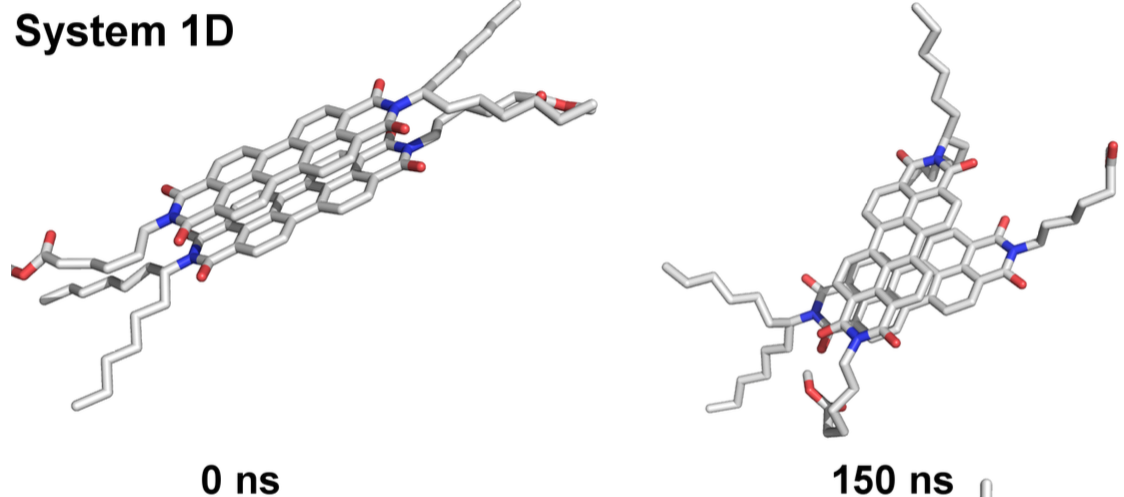
\includegraphics[width=0.45\columnwidth]{image/Figure2a}&
		 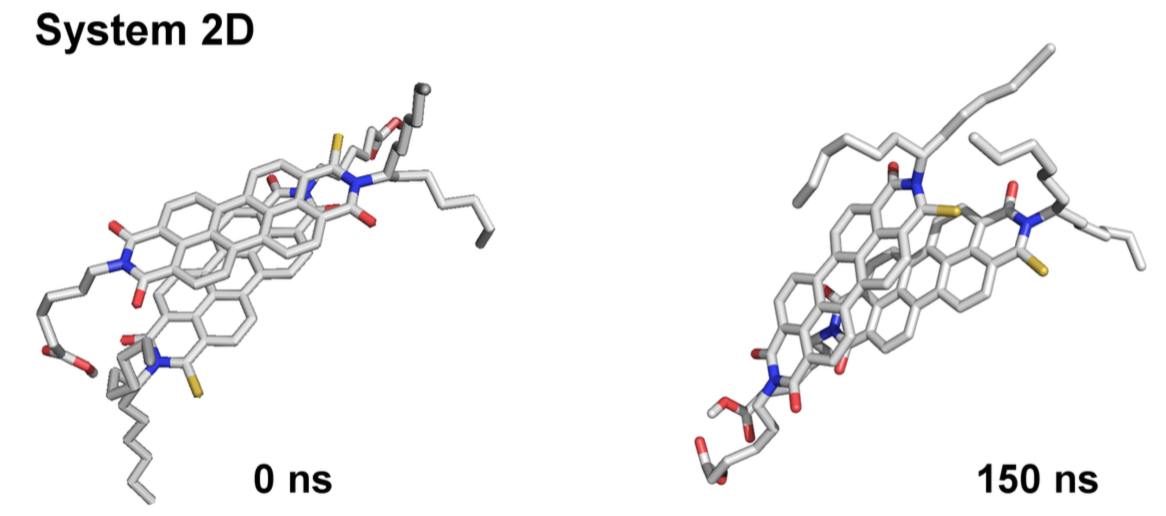
\includegraphics[width=0.45\columnwidth]{image/Figure2b}\\    
		 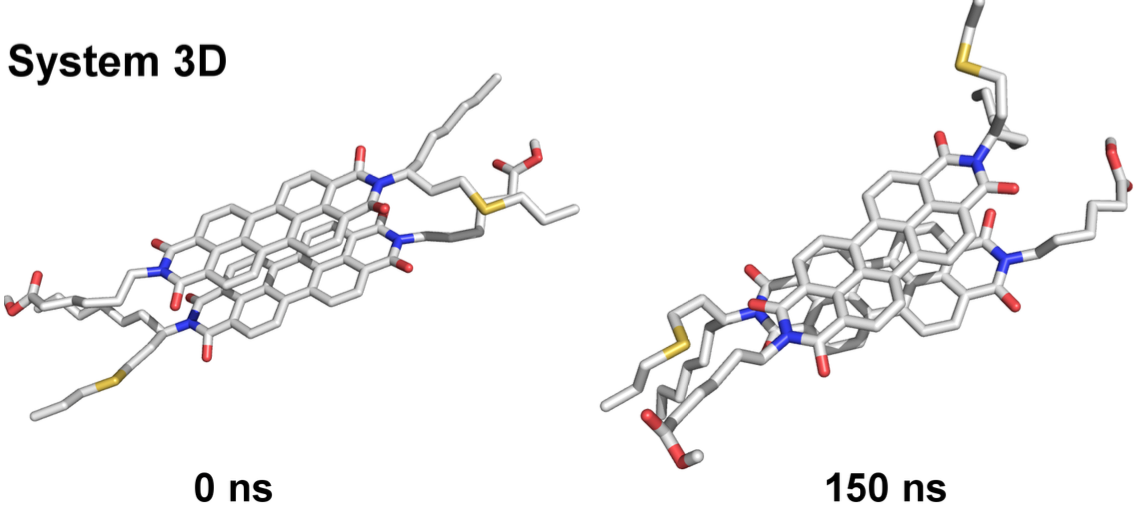
\includegraphics[width=0.45\columnwidth]{image/Figure2c}&     
		 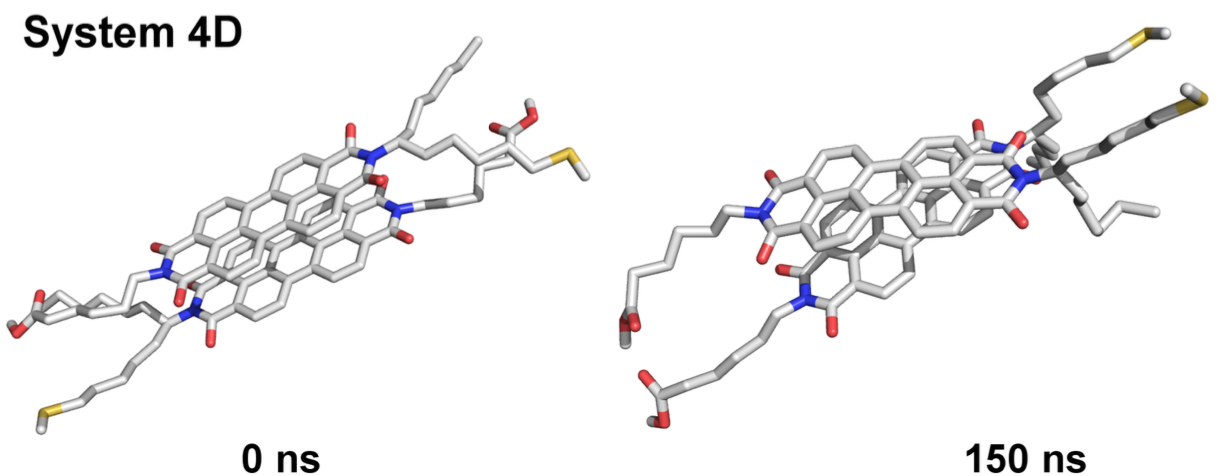
\includegraphics[width=0.45\columnwidth]{image/Figure2d}\\     
		 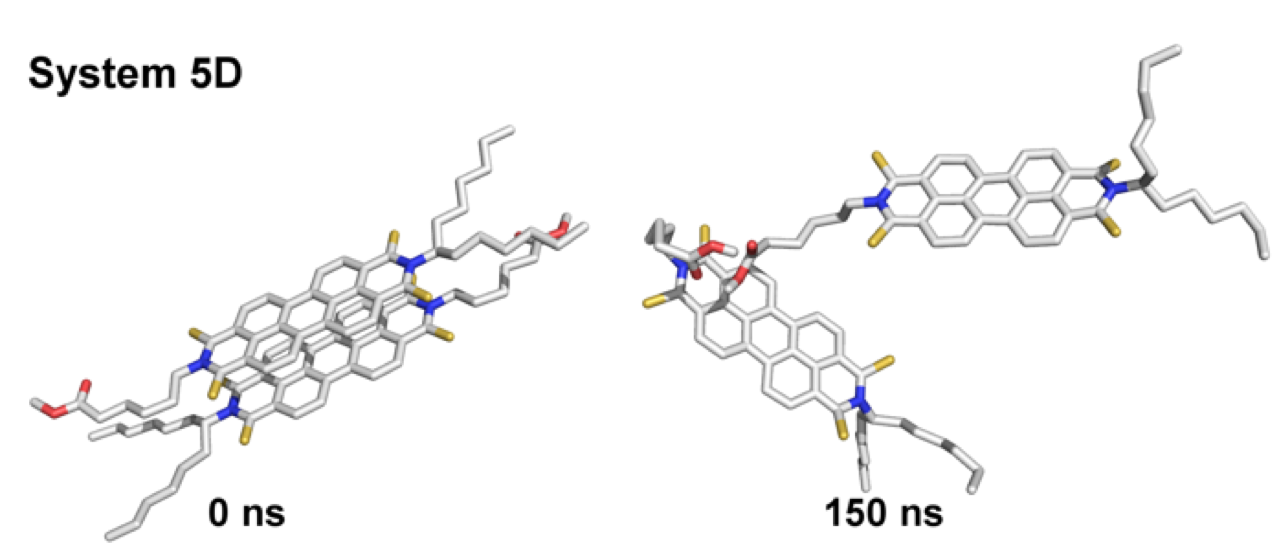
\includegraphics[width=0.45\columnwidth]{image/Figure2e}&
		 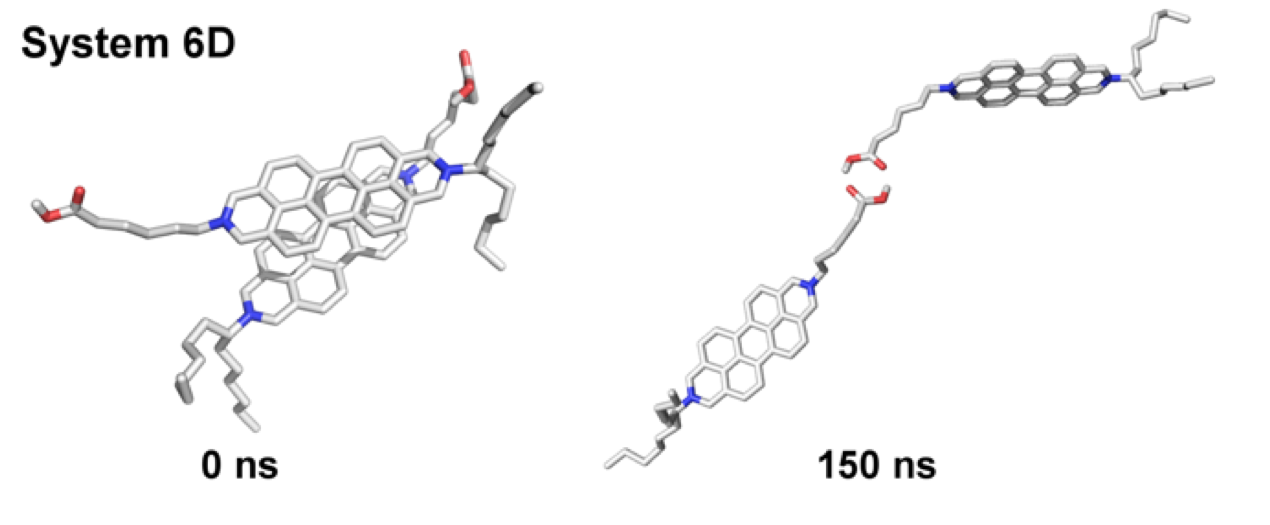
\includegraphics[width=0.45\columnwidth]{image/Figure2f}\\
	\end{tabular}
	\caption{Snapshots of the initial configuration and the final frame of the dimers simulations. Carbon atoms are in grey, oxygen in red, nitrogen in blue and sulfur in yellow. Hydrogen atoms are omitted for clarity.}
	\label{pap:fig03}
\end{figure}

\begin{figure}[htb]
	\begin{tabular}{cccc}
		\small\textbf{System 1D} &  & \small\textbf{System 2D} &\\
		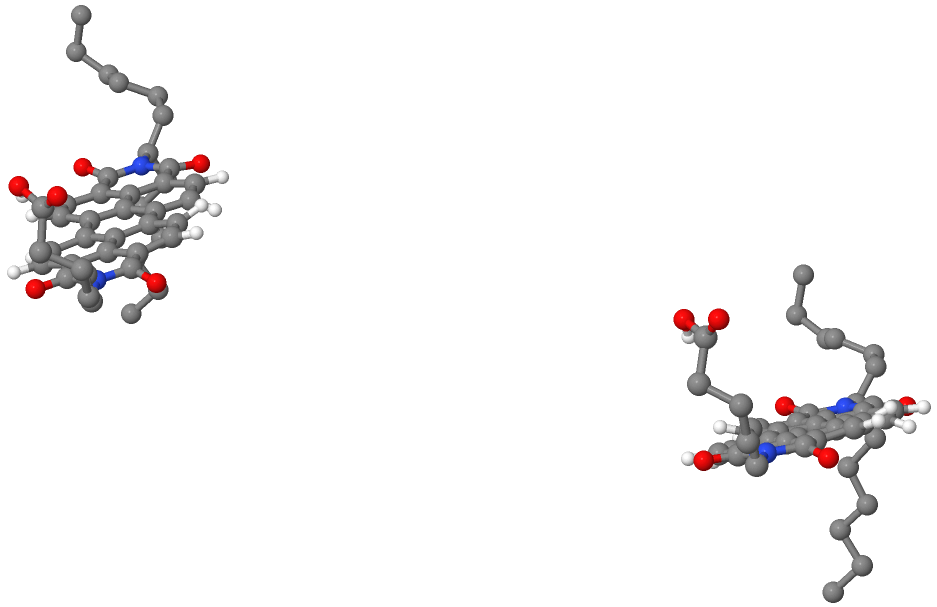
\includegraphics[width=0.2\columnwidth]{image/D_M1_0ns} & 
		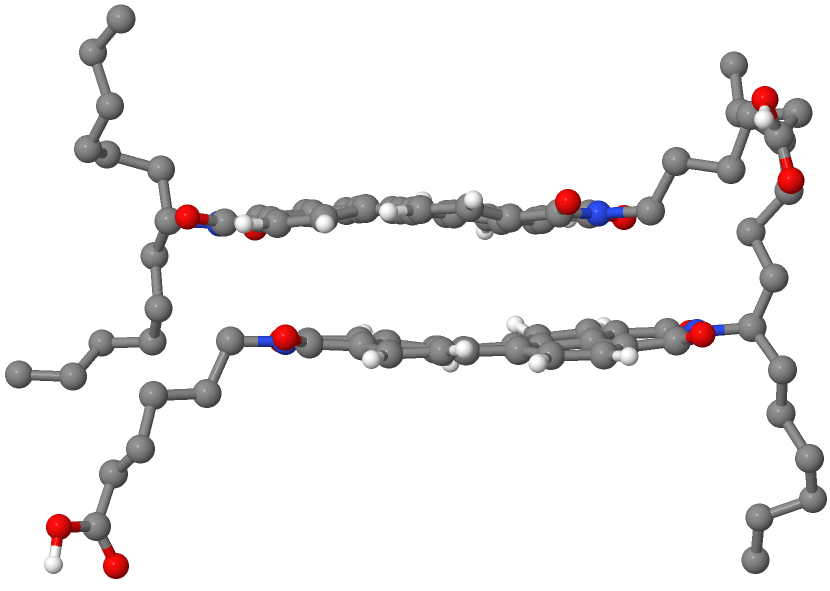
\includegraphics[width=0.2\columnwidth]{image/D_M1_150ns} &
		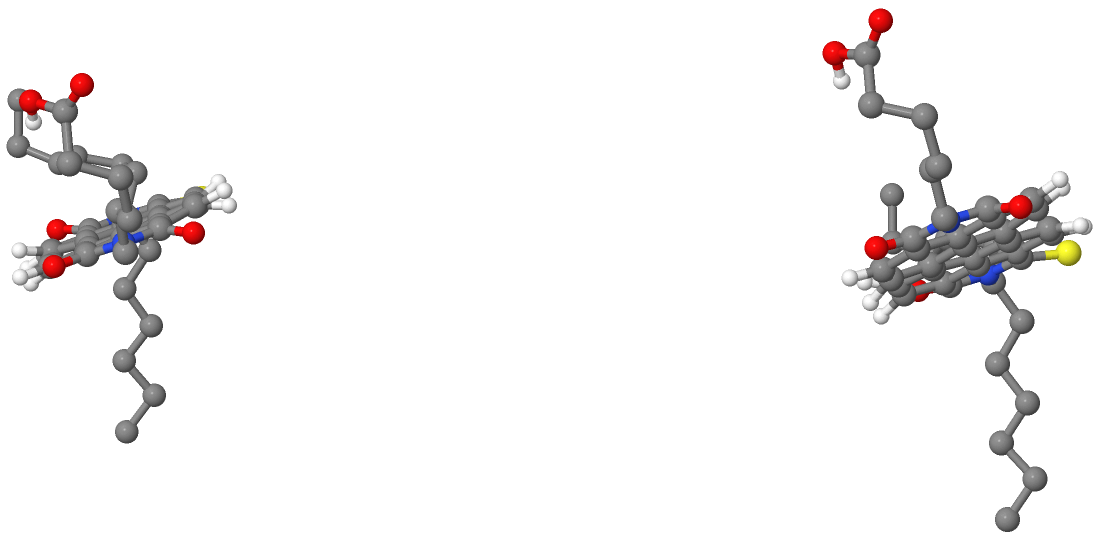
\includegraphics[width=0.2\columnwidth]{image/D_M2_0ns} &
		 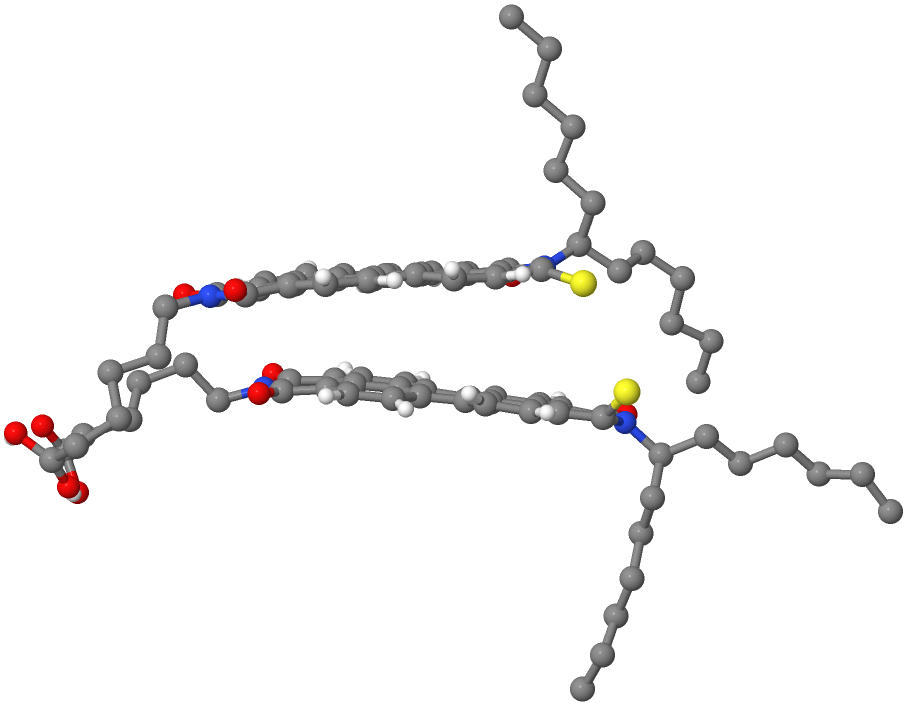
\includegraphics[width=0.2\columnwidth]{image/D_M2_150ns}\\   
		\small\textbf{0 ns} & \small\textbf{150 ns} & \small\textbf{0 ns} & \small\textbf{150 ns} \\
		&&&\\
		\small\textbf{System 3D} &  & \small\textbf{System 4D} &\\
		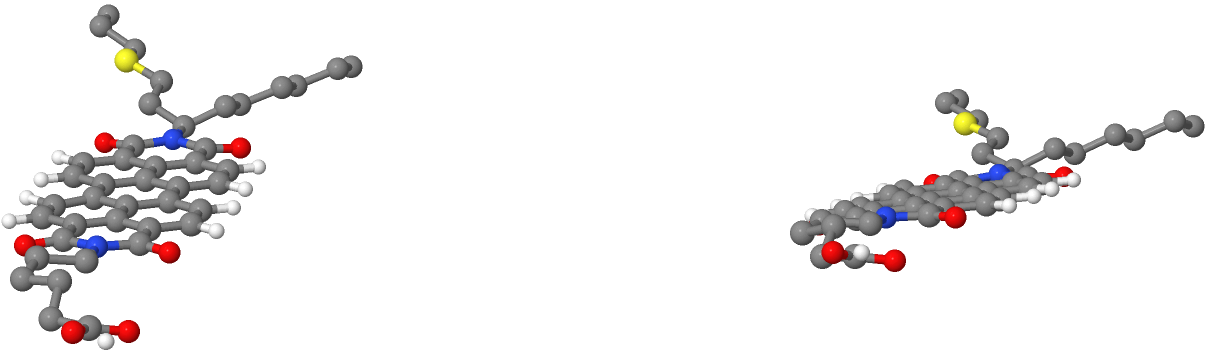
\includegraphics[width=0.2\columnwidth]{image/D_M3_0ns} & 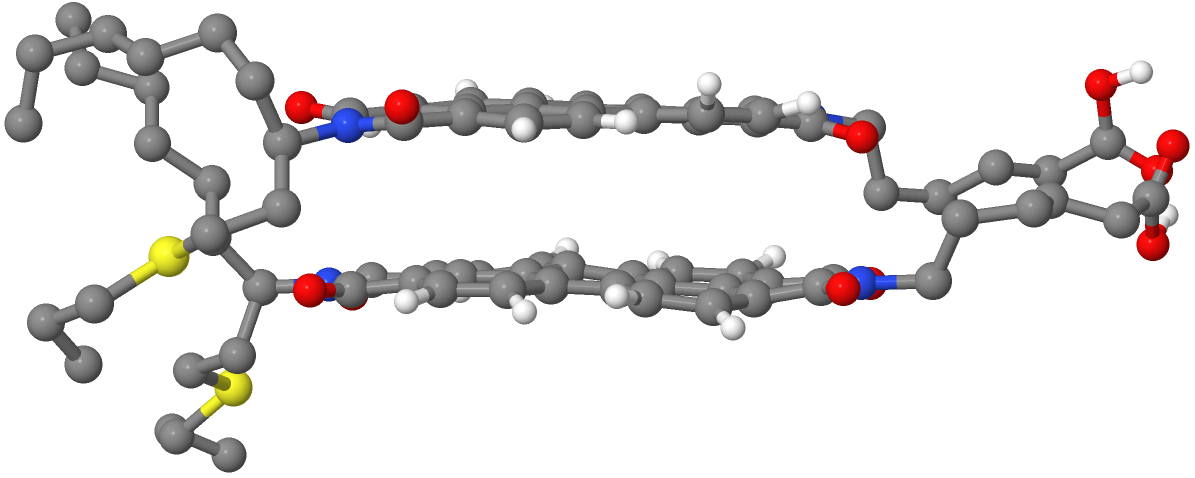
\includegraphics[width=0.2\columnwidth]{image/D_M3_150ns} &
		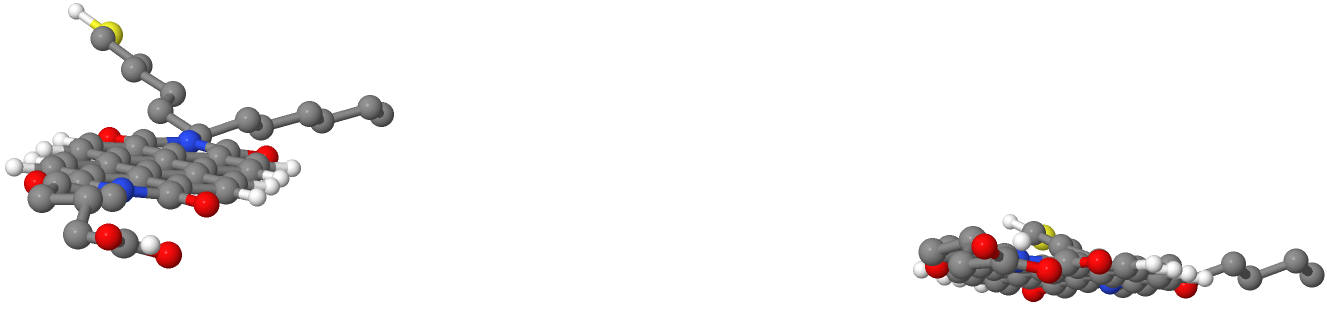
\includegraphics[width=0.2\columnwidth]{image/D_M4_0ns} & 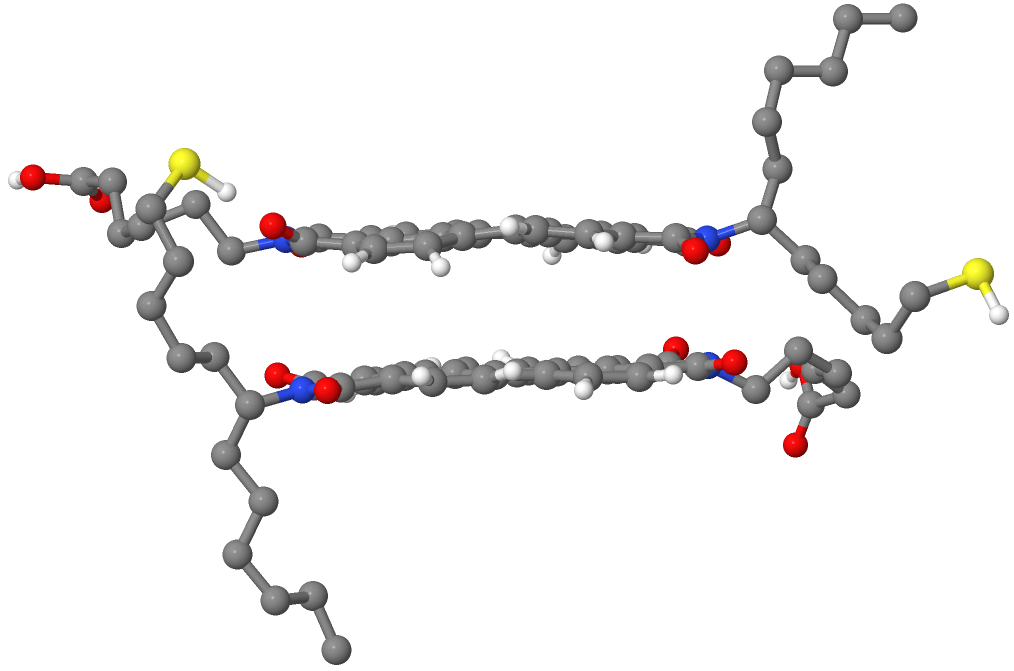
\includegraphics[width=0.2\columnwidth]{image/D_M4_150ns} \\
		\small\textbf{0 ns} & \small\textbf{150 ns} & \small\textbf{0 ns} & \small\textbf{150 ns} \\
		&&&\\
		\small\textbf{System 5D} &  & \small\textbf{System 6D} &\\
		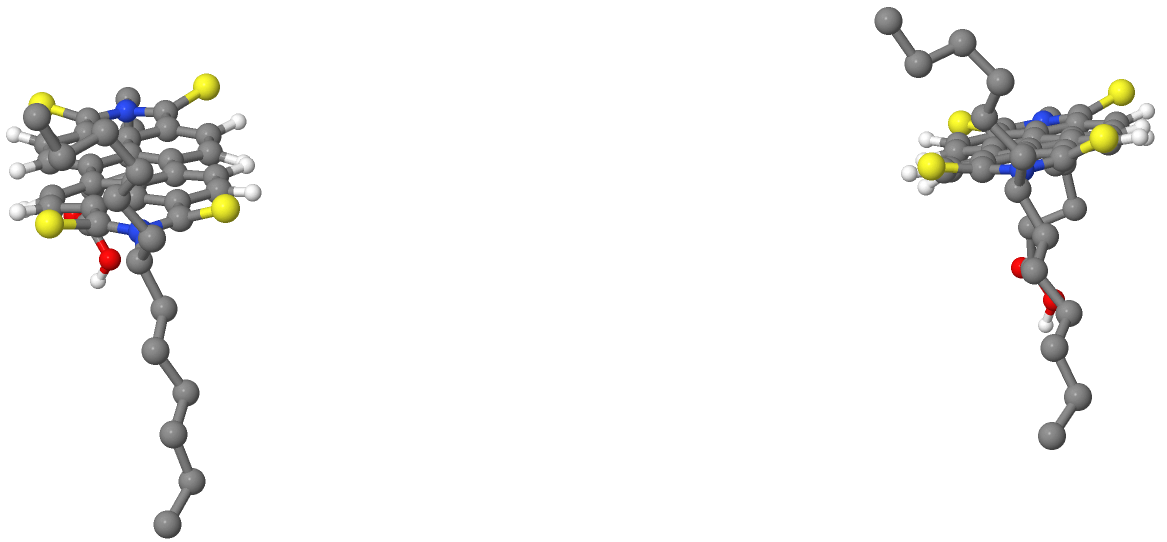
\includegraphics[width=0.2\columnwidth]{image/D_M5_0ns} & 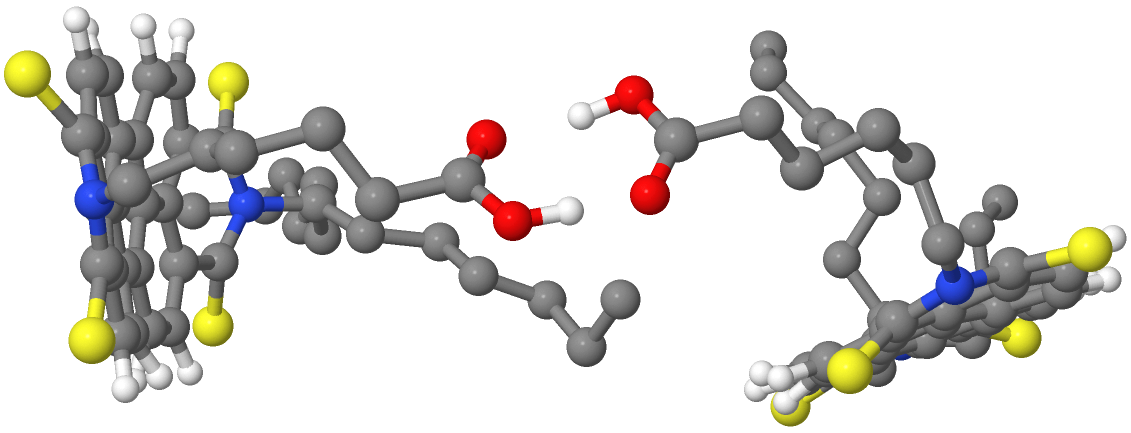
\includegraphics[width=0.2\columnwidth]{image/D_M5_150ns} &
		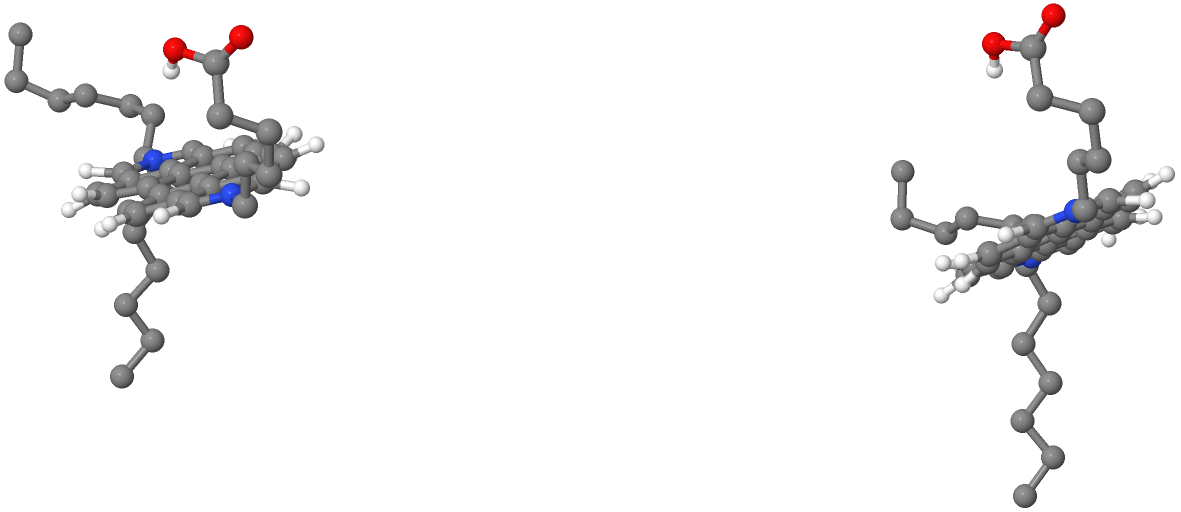
\includegraphics[width=0.2\columnwidth]{image/D_M6_0ns} & 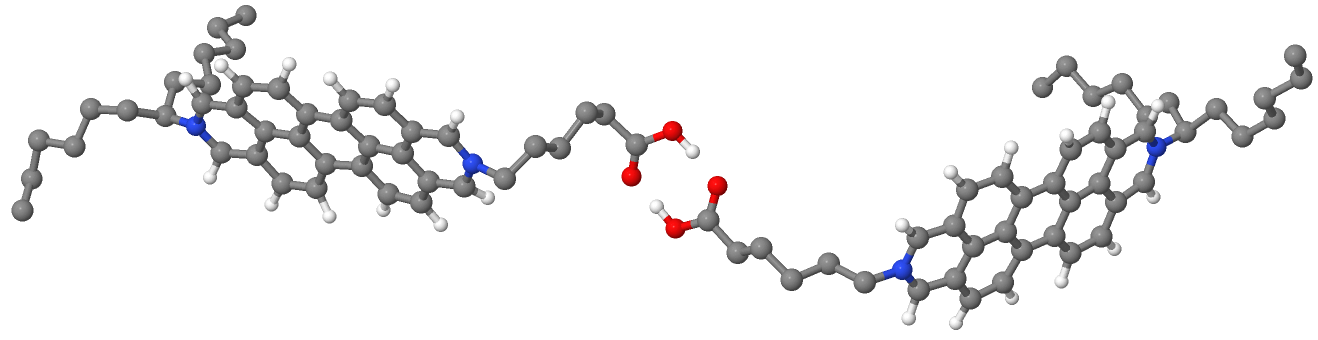
\includegraphics[width=0.2\columnwidth]{image/D_M6_150ns}\\
		\small\textbf{0 ns} & \small\textbf{150 ns} & \small\textbf{0 ns} & \small\textbf{150 ns} \\
	\end{tabular}
	\caption{Snapshots of the initial configuration and the final frame of the dimers simulations for the random disposition case. Carbon atoms are in grey, oxygen in red, nitrogen in blue and sulfur in yellow. Hydrogen atoms are omitted for clarity.}
	\label{pap:fig04}
\end{figure}

\begin{figure}[H]
	\begin{tabular}{cc}
		\includegraphics[width=0.45\columnwidth]{image/Figure3a}&
		\includegraphics[width=0.45\columnwidth]{image/Figure3b}\\
		\includegraphics[width=0.45\columnwidth]{image/Figure3c}&
		\includegraphics[width=0.45\columnwidth]{image/Figure3d}\\
		\includegraphics[width=0.45\columnwidth]{image/Figure3e}&
		\includegraphics[width=0.45\columnwidth]{image/Figure3f}\\                
	\end{tabular}
	\caption{Snapshots of the initial configuration and the final frame of the trimers simulations. Carbon atoms are in grey, oxygen in red, nitrogen in blue and sulfur in yellow. Hydrogen atoms are omitted for clarity.}
	\label{pap:fig05}
\end{figure}

\begin{figure}[htb]
	\begin{tabular}{cccc}
		\small\textbf{System 1T} &  & \small\textbf{System 2T} &\\
		\includegraphics[width=0.2\columnwidth]{image/T_M1_0ns} & \includegraphics[width=0.2\columnwidth]{image/T_M1_150ns} &
		\includegraphics[width=0.2\columnwidth]{image/T_M2_0ns} & \includegraphics[width=0.2\columnwidth]{image/T_M2_150ns} \\   
		\small\textbf{0 ns} & \small\textbf{150 ns} & \small\textbf{0 ns} & \small\textbf{150 ns} \\
		&&&\\
		\small\textbf{System 3T} &  & \small\textbf{System 4T} &\\
		\includegraphics[width=0.2\columnwidth]{image/T_M3_0ns} & \includegraphics[width=0.2\columnwidth]{image/T_M3_150ns} &
		\includegraphics[width=0.2\columnwidth]{image/T_M4_0ns} & \includegraphics[width=0.2\columnwidth]{image/T_M4_150ns} \\
		\small\textbf{0 ns} & \small\textbf{150 ns} & \small\textbf{0 ns} & \small\textbf{150 ns} \\
		&&&\\
		\small\textbf{System 5T} &  & \small\textbf{System 6T} &\\
		\includegraphics[width=0.2\columnwidth]{image/T_M5_0ns} & \includegraphics[width=0.2\columnwidth]{image/T_M5_150ns} &
		\includegraphics[width=0.2\columnwidth]{image/T_M6_0ns} & \includegraphics[width=0.2\columnwidth]{image/T_M6_150ns}\\
		\small\textbf{0 ns} & \small\textbf{150 ns} & \small\textbf{0 ns} & \small\textbf{150 ns} \\
	\end{tabular}
	\caption{Snapshots of the initial configuration and the final frame of the trimers simulations for the random disposition case. Carbon atoms are in grey, oxygen in red, nitrogen in blue and sulfur in yellow. Hydrogen atoms are omitted for clarity.}
	\label{pap:fig06}
\end{figure}

\textbf{Dimers (Systems 1D - 6D)}: The analysis of monomer distances shows that systems 1D through 4D are stable as dimers, regardless the initial configuration within the box (Figure \ref{pap:fig07} and \ref{pap:fig08}). For 1D, the average distance between the two molecules is lower that 0.4 nm during $\sim$ 88\% of the simulation, when the aggregated starting point is used and during 90\% for the random starting point situation. The other systems (2D, 3D and 4D) are also stable and are found in the aggregated state during 85 (96), 94 (98) and 96 (94)\% of the simulation for the ``organized'' (random) starting point. Visual inspection of molecular dynamics simulation (MDS) trajectories indicates that systems 5D and 6D are not stable during the molecular dynamics simulation in toluene and this regardless of the starting configuration. However, the systems presented different behavior. 

For the ``organized'' starting configuration: the monomer from system 5D rotates at the beginning of simulation ($\sim$ 1ns) and becomes separated during the MDS. At system 5T, one monomer rotates at 50 ns followed by side chains interaction. However, this configuration is not stable, since the monomers dissociated after 90 ns. Systems 6D and 6T assume many orientations and remains aggregated during all simulation. Nevertheless, they do not adopt defined geometries. This behavior is typical of an interaction done exclusively by means of the acid chain end via hydrogen bonding. System 5D shows variable distances after 30 ns (Figure \ref{pap:fig07}). The molecules are close to each other (< 0.4 nm) at only 15.4\% (23 ns) of the simulation. System 6D shows instability since the beginning of simulation, with distances higher than 0.4 nm during the simulation time.  

\begin{figure}[htb]
	\centering
	\begin{tabular}{cc}
		\includegraphics[width=0.45\columnwidth]{image/Figure4}&
		\includegraphics[width=0.45\columnwidth]{image/Figure4b}\\
	\end{tabular}
	\caption{Distances between monomers for ``organized'' starting point.}
	\label{pap:fig07}
\end{figure}

\begin{figure}[htb]
	\centering
	\begin{tabular}{cc}
		\includegraphics[width=0.45\columnwidth]{image/distance_1-4}&
		\includegraphics[width=0.45\columnwidth]{image/distance_5-6} \\
	\end{tabular}
	\caption{Distances between monomers for ``random'' starting point.}
	\label{pap:fig08}
\end{figure}

The formation of hydrogen bonds both between two acid chain ends or between an acid chain end and the carbonyl group of the conjugated core are probable to take place for all the 1D-6D systems. One should note that, as it was expected, system 2D has a lower probability of forming such hydrogen bonds interactions because a carbonyl group was replaced by a thionyl one. The same is also true for systems 5D and 6D.\\

The cosine of the angle between the aromatic cores' planes is a useful complementary information towards the determination of the stability of the stack. Values of $\omega = 0^\circ$  (cos $\omega$  = 1) or  $\omega = 180^\circ$ (cos $\omega$ = -1) corresponds to parallel monomers (polyaromatic cores as $\pi-\pi$ stacking), and  $\omega = 90^\circ$ (cos $\omega$ = 0) corresponds to perpendicular molecules (T-shape).\\  

For the ``organized'' starting point, the cosine indicates planar co-facial interacting structures, except for system 1D, which has some fluctuations during the simulation, as it can be seen in Figure \ref{pap:fig09}. For the random starting point, these fluctuations are more common for all the systems in the beginning of the simulation and system 2D has it in the middle of the simulation time. This indicates that, although the parallel co-facial interaction is preferential, as it is also indicated by the minimum distances values, the molecules have some freedom to rotate around their normal axis during the MDS under these thermodynamic conditions. Up to this point, we cannot discern and indicate if this is an effect of the place of the sulfur atom in the structure or if is is just the fact that the hydrogen bonds are dynamic and allow the molecules to rotate. In any case, these results are in agreement with the ones found by Teklebrhan and co-workers.\cite{teklebrhan2012probing} What can be said though is that the 1D-4D systems do not perform T-shape interactions, but this is the case for the system 5D and 6D, as it is reported in Figure \ref{pap:fig10}.

\begin{figure}[p]
	\includegraphics[width=\columnwidth]{image/Figure7}
	\begin{tabular}{cc}
		\includegraphics[width=0.45\columnwidth]{image/Figure7b}&
		\includegraphics[width=0.45\columnwidth]{image/Figure7c} \\
	\end{tabular}
	\caption{Cosine of angle between aromatic cores in function of distance between dimers monomers for the organized starting point. Carbon atoms are in grey, oxygen in red, nitrogen in blue and sulfur in yellow. Hydrogen atoms are omitted for clarity.}
	\label{pap:fig09}
\end{figure}

\begin{figure}[htb]
	\begin{tabular}{cc}
		\includegraphics[width=0.45\columnwidth]{image/angle_1-4}&
		\includegraphics[width=0.45\columnwidth]{image/angle_5-6}\\
	\end{tabular}
	\caption{Cosine of angle between aromatic cores in function of distance between dimers monomers for the random starting point. Carbon atoms are in grey, oxygen in red, nitrogen in blue and sulfur in yellow. Hydrogen atoms are omitted for clarity.}
	\label{pap:fig10}
\end{figure}	

The results obtained previously for systems 5D and 6D are now reproduced if the starting configuration is random. System 5D can assume a stable face-to-face configuration during some periods of the simulation but it is not stable throughout it. System 6D is not stable in this configuration and no stable conformation can be noticed by the distances analysis.\\

\textbf{Trimers (Systems 1T - 6T}: Previous molecular dynamics simulations have shown that molecule 1 (C5Pe) has a high tendency to dimerize in toluene, but it does not form larger aggregates, since it has a long and linear alkyl side chains.\cite{teklebrhan2012probing} However, the distance between the monomers of system 1T is constant from the beginning of the simulation, indicating an average height lower than 0.8 nm.  This is in agreement with experimental work,\cite{eyssautier2011insight} which suggest a height of 0.67 nm. Systems 2T and 4T (after 33 ns) exhibit similar results.\\ 

As it can be seen from Figures \ref{pap:fig11}, \ref{pap:fig12}, \ref{pap:fig13} and \ref{pap:fig14}, the fluctuations in these distances are a function of the starting configuration. In ``organized'' starting configuration, system 3T shows larger distances after 45 ns and the molecules are close to each other ($<$ 0.4 nm) at only 4\% of the simulation. For system 3T, the results show variable molecular dissociation of one monomer, but the remaining dimer is stable. For the random starting configurations, systems 1T and 3T are stable as face-to-face aggregates during almost all the simulation time, whereas 2T takes 75 ns to stabilize in this configuration. The 4T now has the same effect in this situation that 3T had before: the trimer is not stable in the face-to-face configuration although the three molecules are kept together by the hydrogen bonds and the two of them assume the face-to-face configuration, as it is the case of 4D system. 

\begin{figure}[htb]
	\centering
	\includegraphics[width=\columnwidth]{image/Figure8} 
	\begin{tabular}{cc}
		\includegraphics[width=0.5\columnwidth]{image/Figure8b} &
		\includegraphics[width=0.5\columnwidth]{image/Figure8c} \\
	\end{tabular}
	\caption{Distances between monomers for ``organized'' starting point.}
	\label{pap:fig11}
\end{figure}

\begin{figure}[htb]
	\centering
	\includegraphics[width=\columnwidth]{image/Figure10} 
	\begin{tabular}{cc}
		\includegraphics[width=0.5\columnwidth]{image/Figure10b} &
		\includegraphics[width=0.5\columnwidth]{image/Figure10c} \\
	\end{tabular}
	\caption{Angle between monomers for ``organized'' starting point.}
	\label{pap:fig12}
\end{figure}

\begin{figure}[htb]
	\centering
	\begin{tabular}{ccc}
		\includegraphics[width=0.3\columnwidth]{image/distance_M1} &
		\includegraphics[width=0.3\columnwidth]{image/distance_M2} &
		\includegraphics[width=0.3\columnwidth]{image/distance_M3} \\
		\includegraphics[width=0.3\columnwidth]{image/distance_M4} &
		\includegraphics[width=0.3\columnwidth]{image/distance_M5} &
		\includegraphics[width=0.3\columnwidth]{image/distance_M6} \\
	\end{tabular}
	\caption{Distances between monomers for ``random'' starting point.}
	\label{pap:fig13}
\end{figure}


\begin{figure}[htb]
	\centering
	\begin{tabular}{cc}
		\includegraphics[width=0.45\columnwidth]{image/angle_M1} &
		\includegraphics[width=0.45\columnwidth]{image/angle_M2} \\
		\includegraphics[width=0.45\columnwidth]{image/angle_M3} &
		\includegraphics[width=0.45\columnwidth]{image/angle_M4} \\
		\includegraphics[width=0.45\columnwidth]{image/angle_M5} &
		\includegraphics[width=0.45\columnwidth]{image/angle_M6} \\
	\end{tabular}
	\caption{Angle between monomers for ``random'' starting point.}
	\label{pap:fig14}
\end{figure}

When the predominant type of interactions was investigated for the case with the ``organized'' starting point, it was noticed they are constant during the whole simulation for system 1T, 2T, and 4T (Figure 9). Those molecules seem to be stable as a trimer. The interaction between the first two aromatic cores is not influenced when a third monomer is added, which in turn, has an identical behavior with the second molecule. It suggests that the interaction driving the aggregation is made from the poly-aromatic cores. Although, the side chain should contribute to aggregation since it interacts during all the simulation for the four systems. 

The monomers geometries can be also analyzed by the cosine values of the angle between poly-aromatic cores (Figures \ref{pap:fig12} and \ref{pap:fig14}). For all trimer systems, the planar configuration is more likely than others, namely the T-shape. System 3T, in the ``organized'' starting point  (Figure \ref{pap:fig12}) and system 4T in the random starting point (Figure \ref{pap:fig14}) show now variations in these angles, either in the beginning or during the whole simulation. This, added to the fact that the intermolecular distance is similar for both 1-3 and 2-3 molecules, is an indication that the dimer is stable and interacts with the third molecule via the hydrogen bonds. 

The distances between monomers of systems indicate greater variation for system 5T and 6T. System 5T shows larger distances after 30 ns and the molecules are close to each other (< 0.4 nm) at only 13\% (19.5 ns) of the simulation. System 5T shows larger distances during the entire simulation, due to monomers dissociation. The trimers geometry was also analyzed by the cosine values of the angle between poly-aromatic cores. For both systems, the cosine does experience large variation and does not have association to short distances.\\ 

The stable trimers also interact through hydrogen bonds during the simulation. On systems 2T, 3T and 4T, the hydrogen bonds interactions occur basically between carboxylic groups of side chains (Figure 11). For systems 4T, the frequency of these hydrogen bonds is higher than 96\% of the total simulation. For systems 3T, the numbers decrease to 63\%, since only side chains from monomers 1 and 2 interact. Furthermore, only for system 1T, the numbers of hydrogen bonds between the side chains and the carbonyl group of poly-aromatic core are significant (80\%). Moreover, the presence of carboxylic acid groups is important to aggregation, but they were not enough present to maintain the trimer in a parallel orientation, as observed in systems 1T, 3T and 4T (from random starting point).

The side chains from trimers interact through hydrogen bonds during the simulation. At systems 5T, the frequency of hydrogen bonds between carboxylic groups of side chains is higher than 50\% (75 ns) of total simulation, but for system 6T, this number decreases to 26\% (39 ns). Moreover, the presence of carboxylic acid group is important to aggregation, but they were not enough to maintain the aggregated in a parallel orientation.\\


\textbf{General effect of the Sulfur atom}: Up to now, the properties of the aggregates of molecules 1-4 has been discussed for dimers and trimers. Although some differences in their dynamics in solution could be noticed during MDS, no final conclusion on the role of the sulfur hetero-element can be extracted so far. In order to circumvent this shortcut, we have introduced, for the random starting configurations, the study of the radial distribution functions (RDF) for the \ce{S-X} pairwise interactions, where \ce{X} can be: 1 - the oxygen atoms of the aromatic core (aromatic carbonyl groups), 2 - the oxygen atoms of the carboxylic acid group (\ce{COOH}), and 3 - the hydrogen atom of the same group. This was motivated since it is known that sulfur atoms can form non-covalent (Coulomb and/or van der Waals) interactions with oxygen and hydrogen,\cite{jackson2013controlling} sometimes strong enough to lock conformations in place. These graphics can be found in Figure \ref{pap:fig16} for the dimer and \ref{pap:fig17} for the trimer systems.\\

\begin{figure}[htb]
	\begin{tabular}{cc}
		\includegraphics[width=0.45\columnwidth]{image/rdf_14} &
		\includegraphics[width=0.45\columnwidth]{image/rdf_56} \\     
	\end{tabular}
	\caption{Normalized Radial Distribution Functions for the trimer systems.}
	\label{pap:fig15}
\end{figure}	

\begin{figure}[htb]
	\begin{tabular}{cc}
		\includegraphics[width=0.45\columnwidth]{image/rdf_SOar} &
		\includegraphics[width=0.45\columnwidth]{image/rdf_SOcarb} \\
		\includegraphics[width=0.45\columnwidth]{image/rdf_SHcarb} & \\        
	\end{tabular}
	\caption{Normalized Radial Distribution Functions for the \ce{S-X} pairwise interactions, where \ce{X} can be the oxygen atom of the aromatic core, the oxygen atom of the carboxylic group (\ce{COOH}) or its hydrogen for the dimer system.}
	\label{pap:fig16}
\end{figure}	


\begin{figure}[htb]
	\begin{tabular}{cc}
		\includegraphics[width=0.45\columnwidth]{image/rdf_SOar2} &
		\includegraphics[width=0.45\columnwidth]{image/rdf_SOcarb2} \\
		\includegraphics[width=0.45\columnwidth]{image/rdf_SHcarb2} & \\        
	\end{tabular}
	\caption{Normalized Radial Distribution Functions for the \ce{S-X} pairwise interactions, where \ce{X} can be the oxygen atom of the aromatic core, the oxygen atom of the carboxylic group (\ce{COOH}) or its hydrogen for the trimer system.}
	\label{pap:fig17}
\end{figure}	

In dimer and trimer systems, all the peaks found in the \ce{S}-aromatic carbonyl oxygen RDFs are due to intra-molecular configurations. This is known by measuring the \ce{S-O} distances of an isolated molecule of each type. Minor peaks, as it is the case of the ones found around 3, 8 and 14 \AA~for system 2D, are due to the interaction with oxygen atoms of the other molecule interacting with the one bearing the reference sulfur atom. The other systems show similar behavior with wider peaks now due to the fact that sulfur atoms are in flexible parts of the molecule. This allows us to state that there is no particular affinity between sulfur atoms and aromatic carbonyl atoms in the studied structures and this cannot be a likely interaction mechanism.\\

The \ce{S-O} (\ce{COOH}) and \ce{S-H} have now new features that could not be observed in the previous case. Considering both dimer and trimer systems, these two RDFs have intra-molecular peaks centered at around 18 \AA~for molecule 2 (systems 2D and 2T), 22 \AA~for molecule 3 (systems 3D and 3T), and 26 \AA~for molecule 4 (systems 4D and 4T - out of the measurement range, but one can see the peak in the end of the graph). The other peaks are due to inter-molecular interactions between adjacent molecules. Molecule 2, regardless if it is a dimer or a trimer, does not have these additional peaks, indicating that the presence of the sulfur atom on the conjugated backbone does not have any particular affinity with neither oxygen or polar hydrogen atoms of the other molecules. On the other hand, molecule 3 (system 3D) has a ``bump'' for both \ce{S-O} (\ce{COOH}) and \ce{S-H} (\ce{COOH}) RDFs centered at 8 \AA~that does not come from an intra-molecular interaction and is a signature of inter-molecular affinity between the sulfur atom and these oxygen and hydrogen atoms. This behavior is more pronounced in trimer systems, as it expected, since this interaction can take place more easily.\\

This behavior is still more pronounced for molecule 4 (system 4D and 4T): the \ce{S-O} and \ce{S-H} inter-molecular interactions are now very likely to take place and, considering the peak centered in 2.5 \AA~of the S-H RDF that is not present in the \ce{S-O} curve (see Figure \ref{pap:fig09}), one could say that there is also an affinity of this terminal \ce{-SH} group with the acid chain ends of the neighbor molecule. This same characteristic is found for trimer systems (Figure \ref{pap:fig10}).\\

Based on these observations, one can state that sulfur atoms grafted directly to the conjugated backbone has a little influence on the dynamic behavior of dimer and trimer asphaltene systems and one might not be able to differentiate this with what is observed for the case where there is no sulfur atom (molecule 1). Oppositely, the presence of sulfur atoms on the lateral chains, either in the middle of it or as a chain end, has a more pronounced effect on the properties of these molecules (molecules 3 and 4). This is due to the fact that this atom can now interact with acid chain ends of neighbor molecules by means of non-covalent interactions like Coulomb and/or van der Waals.\\

Although the differences herein highlighted can, in our scale, not be of uppermost importance, it is the case in oil industry where huge quantities of molecules are being treated at the same time. These results can help towards the comprehension why crude oils with an elevated sulfur content are more difficult to crack, as a matter of fact. 


\clearpage

\subsection{Schuler's-derivatives systems}

The systems were arranged so that to determine the separated effects of the different heteroatoms and the chain-ends.

\subsubsection{Effect of the heteroatom}

In order to study the effect of the heteroatom on the aggregation process of the PA3-type molecule, we screened the three free positions letting \ce{X} assume the values of \ce{O}, \ce{S} and \ce{NH}. Moreover, the chain-end for this purpose was chosen to be \ce{-CH3} in order to avoid any effect due to hydrogen-bonding on the aggregation mechanism, as it will be studied later on. Thus, the following systems were considered: A13, A23, A33, A43, and A53. Although only one heteroatom is found in family CA22, \textit{i.e.} nitrogen, we also present here, for the sake of comparison, the results obtained for the AAC molecule. In Figure \ref{pap:fig18}, one can find the normalized RDF functions  of these systems under 298 K and 1 bar conditions.

\begin{figure}[h]
	\begin{tabular}{cc}
		\includegraphics[width=0.45\columnwidth]{image/02a} & 	
		\includegraphics[width=0.45\columnwidth]{image/02b} \\
		(a) & (b) \\
	\end{tabular}
	\caption{Aggregation mechanism with \ce{-CH3} ended chains: (a) effect of the heteroatom (A13, A23, A33, A43, A53)  and (b) effect of the asphaltene type (A53/AAC). Each peak of the RDFs corresponds to a neighbor molecule in the $\pi$-stacking structure presented in Figure \ref{pap:fig03}.}
	\label{pap:fig18}
\end{figure}

These curves describe the organization structure in liquid state of the asphaltene solution. Such regular separation between peaks with an interval of around 3.9 \textup{\AA} indicates that the asphaltenes are organized in a stack structure. The first peak centered at $\sim$ 3.9 \textup{\AA} stands for the interactions with the first neighbors generated by the $\pi$-stacking interaction. Depending on the position of the molecule within the stack, it can have one or two first neighbors. The other peaks represent the second, third and fourth neighbors in the stack. In this way, as the RDFs describe a probability density, it is almost twice more probable for an asphaltene to have a first neighbor at 3.9 \AA~than a second neighbor at 7.8\AA.\\ 

Different heteroatom substitution has a slight effect on the shape of the RDFs, although there are intensity changes (not seen here because the normalized version is presented). This is probably due to the fact that the total density of the liquid is slightly changed in function of the heteroatom (as they have different masses and different Van der Waals radii). The most important change concerns the CA22 asphaltene type AAC. This molecule has an aggregation pattern that also follows a stack architecture but high-order neighbors are not as probable as they are for the PA3 type. This is indicative of a short-range order whereas a long-range one is not kept during the simulation. This is evidenced by the snapshots of their molecular architecture after 60 ns of molecular dynamics simulation at 298K and 1 bar in Figure \ref{pap:fig19}.

\begin{figure}[h]
	\begin{tabular}{cc}
		\includegraphics[width=0.45\columnwidth]{image/A33_60ns} & 	
		\includegraphics[width=0.45\columnwidth]{image/AAC_60ns} \\
		(a) & (b) \\
	\end{tabular}
	\caption{60 ns-snapshots of 5 molecules of each asphaltene in toluene at 298K and 1 bar conditions: (a) A33 and (b) AAC. Carbon atoms are presented in gray and nitrogen atoms in blue. Aromatic or polar hydrogen atoms are presented in white. Toluene molecules are omitted for clarity.}
	\label{pap:fig19}
\end{figure}

Whereas PA3-type molecules, regardless of the heteroatom, aggregate forming co-facial planes, CA22-type molecules stack in a not completely planar way, leaving room to the formation of tilted architectures between adjacent molecules. This is the case during the whole simulation. This explains the lower intensity peaks present in the RDF. In order to deeply understand these features, the analysis of the energies of interaction is then a powerful tool to elucidate the effect of changing the heteroatom on the aggregation strength of these molecules. We studied the dimers of each molecule in vacuum dynamics for 10 ns using the same conditions as during the stabilization step. The time-averaged interaction energy $<E_i>$ was determined by:  

\begin{equation}
<E_i>=-(<E^p_d> - 2.<E^p_m>)
\end{equation}

$<E^p_d>$ stands for the average value of the potential energy of the dimers after it has stabilized and $<E^p_m>$ is the average value of the potential energy of a single isolated molecule after it has stabilized. The same method of calculation has been used by Liu \textit{et al.}\cite{liu2015molecular} The interaction energies of PA3 and CA22 dimers in vacuum, reported in Table \ref{pap:tab02} (diagonal values), corroborate the interpretation extracted from the analysis of the RDF functions: for any given molecular structure within the same class, changing one heteroatom by another has a slight effect on these molecules' dimers aggregation. The energies of interaction fluctuate around the average value of 55.7 kcal.mol$^{-1}$ (3.8x10$^{-19}$J) for the PA3 class of molecules. For the CA22 molecule type, the interaction energy is lowered by around 10 kcal.mol$^{-1}$. The out-of-diagonal values reported in this Table will be discussed in the next sections.

\begin{table}[h]
	\centering
	\begin{tabular}{c|cccccc}
		\hline
		& A13 & A23 & A33 & A43 & A53 & AAC \\
		\hline         
		A13 & 56.2 & 40.9 & 37.4 & - & - & 42.2 \\        
		A23 & 40.9 & 52.2 & 46.7 & - & - & 47.4 \\
		A33 & 37.4 & 46.7 & 57.0 & - & - & 35.2 \\
		A43 & - & - & - & 58.9 & - & - \\
		A53 & - & - & - & - & 54.0 & - \\
		AAC & 42.2 & 47.4 & 35.2 & - & - & 45.8 \\
		\hline
	\end{tabular}
	\caption{Interaction energies ($<E_i>$) in kcal.mol$^{-1}$ calculated for PA3- and CA22-type dimer molecules.}
	\label{pap:tab02}
\end{table}

One should keep in mind that these molecules present different contributions of the Van der Waals and the Coulomb terms to the potential energy. Whereas one should expect the Van der Waals energy term to be higher for molecules containing Sulfur atoms than molecules containing Nitrogen and Oxygen atoms (motivated by the increase of the C$_6$ and C$_{12}$ Van der Waals terms, respectively). On the contrary, the Coulomb terms involving Oxygen should be higher than Sulfur's and Nitrogen's, motivated by the increased local dipole moments. In this way, the interaction energies result of both effects taking place at the same time, besides other contributions due to the angle, dihedral and improper torsion terms that are not equivalent elsewhere. The Van der Waals interactions are understood as the combination between Lennard-Jones repulsion terms (with a $r^{-12}$ dependence) and the London dispersion/attractive terms, which is originated from induced dipole-induced dipole interactions (with a $-r^{-6}$ dependence). Finally, it is worth noting that the Coulomb interactions, besides having a repulsive/attractive $r^{-1}$ character, occur between fixed dipoles/charges-fixed dipoles/charges.\\

Decomposing the total potential energy in these terms, we found that the highest contribution to the interaction energy comes from the non-bonding Van der Waals potential terms. These contributions represent 86, 81, 84, 85, 82 and 73 \% of the total interaction energy for A13/A13 ... AAC/AAC interaction pairs, respectively. The Coulomb energy contributions are not higher than 4\%. This result indicates that, for the situations where a molecule interacts with a similar one, the Van der Waals forces govern the aggregation between the adjacent molecules. 

\subsubsection{Effect of chain-end}

Having such results in mind, we studied the presence of \ce{-COOH} functions on the chain-ends for the same molecules under the same conditions, for A11, A21, A31, A41, A51 and AAA. Molecules A12 and AAB are presented in a separate plot that can be found in the ESI. The normalized RDF functions for these systems can be found in Figure \ref{pap:fig20}.

\begin{figure}[h]
	\begin{tabular}{cc}
		\includegraphics[width=0.45\columnwidth]{image/04a} & 	
		\includegraphics[width=0.45\columnwidth]{image/04b} \\
		(a) & (b) \\
	\end{tabular}
	\caption{Aggregation mechanism with \ce{-COOH} ended chains: (a) effect of the heteroatom (A11, A21, A31, A41, A51)  and (b) effect of the asphaltene type (A51/AAA). Each peak of the RDFs corresponds to a neighbor molecule in the $\pi$-stacking structure presented in Figure \ref{pap:fig19}.}
	\label{pap:fig20}
\end{figure}

The RDFs differ significantly from the previous case with no acid chain: they are characteristic of liquids where the aggregates concern the stack of only two molecules, longer stacks presenting a lower probability. The interactions are now governed by another mechanism and the structure of the aggregate is less ordered in comparison to the stack structure, probably due to the presence of H-bonds, which signature can be seen as the 2 \textup{\AA} small peaks. The acid chain-ends have an effect of overwhelming the $\pi$-stacking interactions beyond the second neighbor, hiding the third- and fourth-neighbor peaks.\\

The loss of symmetry due to the formation of H-bonds is identified in the RDFs by the wide peaks appearing for lengths superior to 10 \textup{\AA}. This wide peak is attributed to the interaction between asphaltene aggregates that are not rigid and have gained degrees of freedom from the presence of the H-bonds. Moreover, these wide poorly-defined bands can hide underneath it the peaks due to $\pi$-stacking aggregation. This can be visualized in the snapshots of A31, AAA, A33 and AAC presented in Figures \ref{pap:fig19} and \ref{pap:fig21}.

\begin{figure}[h]
	\begin{tabular}{cc}
		\includegraphics[width=0.5\columnwidth]{image/A31_60ns} & 	
		\includegraphics[width=0.5\columnwidth]{image/AAA_60ns} \\
		(a) & (b) \\
	\end{tabular}
	\caption{60 ns-snapshots of 5 molecules of each asphaltene in toluene at 298K and 1 bar conditions: (a) A31 and (b) AAA.}
	\label{pap:fig21}
\end{figure}

Interestingly, the formation of H-bonds are stable enough under these conditions to avoid the self-stacking as it is the case of the \ce{-CH3}-ended molecules. This characterizes the formation of an elongated cluster in the presence of more than five molecules and could also be responsible for forming larger clusters more rapidly. The interaction energy of two $n$-hexanoic acid chains alone was calculated under the same conditions as before and we have found it to be as high as 22 kcal.mol$^{-1}$ for each pair of \ce{-COOH} groups. When decomposed, this energy is consisted of a balance between the Coulomb and Van der Waals interactions. The intensity of the binding character of Coulomb interaction is around 10 times bigger than the repulsion character of Van der Waals interaction.\\ 

This result shows that the presence of acid chain-ends and the consequent formation of H-bonds within the crude oil is also a great aggregation factor. This can explain why these molecules are so difficult to treat in oil industry's production chain. Total interaction energies can be estimated to be as high as 75 kcal.mol$^{-1}$, including both the $\pi-\pi$ and a pair of H-bond interactions, as aforementioned. Such a strong interaction between two adjacent molecules is almost equivalent to a covalent bond. For larger aggregates, this energy should be multiplied by the number of aromatic cores in interaction and the total number of acid chain-ends.\\

As it has been reported experimentally,\cite{durand2010effect} the macro-aggregates should be linked to each other by weak dispersive interactions between their lateral chains or simply because they are more polar than their environment, causing that they remain close together. This should explain why, experimentally, stirring the sample is enough to separate these aggregates in smaller pieces. In an underneath scale, the interactions should be governed by H-bonds which are much more robust and should keep the nano- and/or micro-aggregates in place. Finally, the same H-bonds and the $\pi$-stacking between the conjugated planes as herein studied are supposed to be the interactions ruling the aggregation phenomena at the nano-scale. This multi-scale model of the organization of asphaltene aggregates was first proposed by Mullins \textit{et al.}\cite{mullins2010modified,mullins2011asphaltenes,mullins2012advances}

\subsubsection{Aggregation within heterogeneous boxes}

Next, we will present the results of aggregation for boxes containing different asphaltenes, be it the same family or not. For the simulation of the mixtures between asphaltenes of the same family, we continued on using the same conditions but varied the relative concentration between the constituents.\\

As it was aforementioned, the effect of the heteroatom on the asphaltene aggregation with a given family can be considered as important as the difference of energies between two different classes of them. This means that, the effect of the heteroatom cannot be, at this point, ignored since the difference in energy found when changing it with a the same family of molecules (say A13 and 133) is of the same order of magnitude of the energy difference found when the asphaltene family is changed (say A13 and AAC). But, as a single model cannot be formulated to capture the effect of all the possible combination of heteroatoms, we excluded from now on the structures containing two different heteroatoms on the conjugated core of the same molecule (A41, A43, A51 and A53). This allows us to still have a large variety of possible combinations.\\

Firstly, we study the binary mixtures within the PA3 molecular family. The combinations were done in order to screen the effect of relative concentration keeping constant the total number of five molecules within the simulation box. The concentrations were screened replacing a molecule of one type of asphaltene by another one at a time. This scheme is better understood after seeing Table S2 in the ESI (Mix 1a to 1d).

The simulation of these systems produces two different RDFs: the self-interaction and the cross-interaction curves. The first one describes the probability of any given molecule to interact with a system of the same nature during the simulation and the second one describes the probability of interaction between two different molecules. The curves for the A13:A23 mixture are presented in Figure \ref{pap:fig22}. A13:A33 and A23:A33 mixtures can be found in Figure S1. 

\begin{figure}[htb]
	\centering
	\includegraphics[width=0.4\columnwidth]{image/06a} 
	\caption{Effect of the mixture of A13 and A23 asphaltene molecules with \ce{-CH3} lateral chain-end. This mixture concerns different ratios between Oxygen and Sulfur in the nano-aggregate.}
	\label{pap:fig22}
\end{figure}

These curves indicate that, regardless of the heteroatom, the asphaltenes have similar aggregation mechanisms, \textit{i.e.}, the self-aggregate forming $\pi$-stacks with equidistant separation. This is represented by the peaks in the RDFs. As a matter of fact, A13 has the same interaction pattern with itself regardless of the concentration of A23 and the same is also valid for A23. This is an indicative that the presence of an asphaltene containing a different heteroatom on the backbone does not interfere on the aggregation of the parent molecule. Furthermore, the fact that not all the peaks are present for a given pair of molecules, e.g. A13-A13, indicates that the reference molecule has no similar to it as a first neighbor but it does have one as a second neighbor, what means that the asphaltenes are randomly intercalated among each others. Similarly, when the reference is A13, for instance, the probability of having A23 neighbors increases with the increase of A23 concentration, as it is expected. These very same conclusions can also be found for the other mixtures, concerning oxygen and nitrogen and sulfur and nitrogen ones.  This allows one to say that, on the basis of these results, the aggregates formation is similar regardless of the combination among the heteroatoms. The major differences in these curves are originated from the random intercalation of the different molecules in the formation of the stack. 

As previously, in order to discriminate if there is indeed any difference in the nano-aggregation process, the energies of interaction between each different asphaltene were studied and they are presented in Table \ref{pap:tab02} (off-diagonal values). It can be seen that the pairwise interaction energy changes for different combination of asphaltenes, \textit{i.e.}, every molecule interacts more strongly with an identical molecule than with a different molecule. This effect might be directly associated to the Coulomb and Van der Waals interactions between these molecules. Upon mixing, the Van der Waals energies are expected to reduce. This is a consequence of the combination rule used to determine the Van der Waals coefficients \ce{C6} and \ce{C12} of two distinct $i,j$ atom pair ($C^{6,12}_{ij}=\sqrt{C^{6,12}_i \times C^{6,12}_j}$) induces that the cross-interactions coefficients to be smaller than the original ones. 

\section{Conclusions}

Several asphaltene structural models have been proposed in the literature, such as the C5Pe molecule. Based on experimental work of Eyssautier and co-workers,\cite{eyssautier2011insight} we have chosen six different model molecules for investigating the role of the sulfur atom position within the asphaltene structure. The molecular dynamics simulations have allowed understanding the stability of asphaltene dimers and trimers in toluene as well as showing that the position of the sulfur atom has an effect on the intermolecular non-covalent interactions that can take place in these systems.\\ 

Although the polar side chain is important for determining the aggregation, the main interactions between the molecules are produced by the poly-aromatic cores, which are responsible to the parallel orientation of molecules. This geometry is confirmed by the cosine of angles between the poly-aromatic cores. 
We suggest that the presence of one sulfur atom in the poly-aromatic core (molecule 2) do not prevent the aggregation, since systems 2D and 2T are stable and the radial distribution functions of the pairwise interaction of this atom and the oxygen atoms of the neighborhood do not show any particular affinity. However, the presence of four sulfur atoms in poly-aromatic core avoids the molecules aggregation in a major part of the simulation and this may be due to both steric hindrance, Coulomb repulsion between sulfur and nitrogen atom of the adjacent molecule. Moreover, this molecular structure can not form hydrogen bonds between the acid chain end and the conjugated core of the molecule. On the other hand, sulfur atoms in the middle of the aliphatic chain, as well as a chain end, have a measurable effect on the stability of both dimers and trimers and this is due to the fact that they have a low, still measurable, interaction with the acid chain end oxygen and hydrogen atoms. Finally, these results can help towards the comprehension why heavy crude oils containing high values of sulfur are experimentally more difficult to treat and to crack.\\

Secondly, we have also studied the effect of mixing different asphaltene molecules on their nano-aggregation and which screening was based on experimentally isolated and identified molecules by Schuler and co-workers.\cite{schuler2015unraveling} Molecular dynamics simulations were used in order to identify the nano-aggregation in homogeneous, heterogeneous and \textit{super}-heterogeneous boxes. The first one consisted of only a type of asphaltene at a time; the second one had, within the same class, different asphaltenes mixed for different concentrations varying the heteroatom and the presence of acid chain-ends; and the third type included the mixing of asphaltenes of different classes with variation of the relative concentration. It seems that the nano-aggregation of these molecules is dependent on the heteroatom on the conjugated core and is more dependent on the chain-end and conjugated core size. The energies of interaction for each mix were calculated and are of the same order of magnitude. However, the energy of interaction between the same type of asphaltene tends to be always higher than the energies between different types and/or classes of molecules. The contribution of the acid lateral chains to the interaction energy was calculated and found to be as high as 22 kcal.mol$^{-1}$. Moreover, changing the heteroatom can induce changes up to 10\% of the total interaction energy if compared to other heteroatom. Finally, one should conclude that the aggregation mechanism might be much more strongly correlated to the size of the conjugated aromatic core and the size and nature of lateral chains than the presence of a particular heteroatom. These results are of great importance to oil industry and can help understanding how the molecular cartography of asphaltene molecules can induce stronger interactions or not. 
%\newgeometry{textwidth=16cm}
\chapter[Phonon calculation]{Acenes}
\minitoc
\restoregeometry

\newpage

\section*{Introduction}
\markright{INTRODUCTION}{}

The strategy in the present work is to perform high-precision quantum mechanical calculations based on harmonic (solid state) ahrmonic (gaz phase) electrical and mechanical approximations to compute spectra for individual molecules and dimers. With the anharmonic approach, unscaled computed outcomes including harmonics, overtones, combinations, intermolecular vibrations and other details of spectra can be compared directly with experimental data. The detailed identification of bands in experimental vibration spectra for crude oils and oil fractions may eventually permit the identification of the presence of members of a family of molecules, and the determination of the significance of specific types of molecular interaction arising in these fluids through spectral decomposition. Potential impacts include: improved speciation, and hence fluid characterization; and improved understanding of association phenomena, such as $\pi-\pi$ interactions, and hence transport property prediction.\\ 

Acenes, a family of linear polynuclear aromatic compounds possessing only $\pi-\pi$ interactions, for which high precision experimental data are available up to pentacene \cite{michaelian2012far}, comprise a benchmark example that illustrates both the potential and the computational challenges found in this line of inquiry. In this respect, various calculation hypotheses used for these large molecules are presented, together with the impact of these calculation hypotheses on the quality vis-à-vis experimental data and the computational cost of vibrational spectra.\\

Spectral assignments, determined on the basis of both wavenumber and relative intensity values, are made primarily using computed spectra for individual molecules, and dimers. In addition, based on experimental observation assessing the presence of deformed molecules in tetracene and pentacene crystals, impact on vibrational spectra of these deformations is evaluated and the phonon spectra is evaluated for the tetracene system. For some cases, assignment ambiguity is only resolved by tracing trends for vibration modes for the acene family as a whole. In the exposition that follows, each of these topics is tackled sequentially. Calculations with tetracene and pentacene monomers (individual molecules) are treated first. Then calculations for dimers and the acene family collectively are treated, and the results synthesized.

\section{Calculation of vibrational spectra of Tetracene and Pentacene Monomers: Comparison with experimental data}

\subsection{Experimental data}

Experimental solid-state infrared spectra of tetracene and pentacene \cite{michaelian2012far} were acquired at room pressure and temperature. The measurements were performed on as received samples. Thus the crystallinity as well as the possible presence of defects in these solids are unknown. For tetracene, two crystal structures have been detected by x-ray diffraction experiments \cite{venuti2004phonons}. At room temperature and pressure, tetracene is triclinic \cite{campbell1962crystal} with space group P\={1}. The unit cell contains two independent molecules at the $(0,0,0)$ and $(1/2,1/2,0)$ inversion sites. Pentacene possesses two polymorphs \cite{venuti2002probing,brillante2005characterization}. One comprises a triclinic layered structure with a herringbone arrangement in the layers, with two equivalent molecules per unit cell \cite{campbell1961crystal}.  The other, commonly found at room temperature, adopts a 14.1 Å d(001)-spacing morphology with an inversion center on both molecules in the unit cell \cite{holmes1999nature,siegrist2001enhanced,mattheus2001polymorphism,mattheus2003identification,mattheus2003modeling}.

\subsection{Computational details: construction of the potential energy surface}

The Becke Three-Parameters Hybrid Functional (B3LYP), a combination of the Becke three-parameter exchange functional (B3) \cite{becke1993density} that includes a mixture of Hartree-Fock exchange with the density functional theory (DFT) exchange-correlation and the LYP correlation functional \cite{lee1988development}, has proven to be a reasonable choice for predicting geometries of aromatic molecules \cite{bauschlicher1995comparison,tirado2008performance}.  Stephens et al. \cite{stephens1994ab} showed that the B3LYP force field yields infrared spectra in very good agreement with experimental data. It has become a standard method for studying vibrational spectra of organic molecules (in the far- and mid- Infrared) in the gas phase \cite{bauschlicher1997calculation,gohaud2005vibrational}. Although the B3LYP method coupled with a sufficiently large basis set is a good candidate to study vibrational spectra of polynuclear aromatic molecules \cite{michaelian2012far}, this standard DFT calculation approach fails to describe long-distance interactions. Consequently, it does not reproduce spectra of interacting molecules \cite{becke1993density,stephens1994ab,kristyan1994can,hobza1995density} where the interpretation of experimental vibration spectra requires consideration of both isolated and interacting molecules.\\

 In parallel to the development to ab initio methods, some progress has been made on implementing the London dispersion force effect into DFT methods, permitting calculations with larger individual molecules and binary pairs. Although the CCSD(T) method in combination with a sufficiently flexible basis set is the most accurate method for reproducing rotation-vibration spectra and to describe intermolecular complexes between aromatic hydrocarbons \cite{begue2006new}, such calculations are impractical for the description of large molecules \cite{begue2012nitrile}. The MP2 method \cite{pople1979derivative}, also able to handle dispersive interactions such as $\pi-\pi$ stacking \cite{chalasinski2000state,johnson2006structure},is a computationally intensive and inadequate method for large molecules too \cite{eilmes2012theoretical}. Chai et al.78  developed a functional based on optimized long-range corrected hybrid density functionals \cite{chai2008systematic}, which employs 100\% Hartree-Fock (HF) exchange for long-range electron-electron interactions, $\omega$B97X, to which they added an empirical dispersive interaction correction \cite{eilmes2012theoretica}. This method was tested by Salzner et al \cite{salzner2011improved} for $\pi$-conjugated oligomers and it overcame the difficulties encountered with standard DFT functionals when dealing with interacting $\pi$-systems.\\
 
 In this work, for isolated molecules and dimers, extended basis-sets consisting of atomic orbitals expressed as fixed linear combinations of Gaussian functions are employed for the calculations.  A split valence 6-311G and 6-311G(p,d) \cite{krishnan1980self,frisch1984self} was needed to provide correct calculation outcomes for naphthalene monomer \cite{saeki2006theoretical}. Validation tests for the $\omega$B97X-D/6-311G calculation method were also performed. The accuracy of DFT calculations in predicting molecular geometries and vibrational frequencies depend on the density functional employed. Thus geometrical optimizations were performed for isolated tetracene, using the $\omega$B97X-D functional as well as the more conventional B3LYP method. The computational results are benchmarked using experimental data obtained by Campbell et al.\cite{campbell1962crystal}.\\
 
 The solid state calculations in the present work were carried out with the use of two approaches:
First, the calculations were carried out with the projector augmented wave (PAW) implementation of Vienna Ab initio Simulation Package (VASP)\cite{kresse1996efficient}. The generalized gradient approximation (GGA) in the PBE parameterization was considered as the exchange correlational functional \cite{perdew1996generalized}. Structural optimizations (triclinic tetracene crystal) were achieved by setting the convergence criteria for total energies are below $5*10^{-6}$ eV, residual forces to be less than $1*10^{-3}$ eV/Å, and stresses limited to 0.02 GPa. To correct the missing dispersion interactions, we have used several recently proposed methods such as PBE functional with pair potential methods D2, D3 (BJ), TS, and TS+SCS. The details of the implementations and usage of these methods can be found elsewhere \cite{grimme2006semiempirical,grimme2011effect,tkatchenko2009accurate,tkatchenko2012accurate,dion2004van}. To obtain accurate band gaps, we have used the GW approximation86.  For getting accurate quasiparticle eigenvalues, we used 200 bands for the summation over the bands in the polarizability and the self-energy formulas, and the polarizability matrices were calculated up to a cutoff  of 200 eV.\\ 
Second, periodic calculations for tetracene were also performed in order to calculated IR intensities with CRYSTAL14 program\cite{dovesi2014crystal14}, using PBE functional and STO-6G (Pople's STO-6G) basis set. Default criteria were used as consider accuracy and SCF convergence. Vibrational frequencies at the $\Gamma$ Point were calculated for the optimized geometry. The empirical dispersion correction by Grimme \cite{grimme2006semiempirical} was performed to take into account weak interactions. 

\subsection{Geometrical parameters of isolated tetracene molecule optimized using B3LYP and $\omega$B97X-D methods associated with 6-311G and 6-311G** basis set}

Geometry optimizations were performed using two different DFT methods (B3LYP and $\omega$B97X-D) implemented in Gaussian 09 software \cite{frisch2009gaussian}, and two basis sets (6-311G and 6-311G**). While Saeki et al. \cite{saeki2006theoretical}  reported a change of symmetry for the naphthalene molecule, from D$_{2}$h to C$_{2}$h (based on MP2/6-311G calculations), optimized geometries for the tetracene molecule, which also possesses D$_{2}$h symmetry, remained planar with D$_{2}$h symmetry in all cases. Calculated bond lengths based on different levels of theory are listed in Table 1 along with their mean deviations from experimental measurements (see also Figure A1 in the supplementary data). For these calculations, irrespective of the level of theory or the basis set employed, the agreement between computed bond lengths and experimental values is very good. The mean deviation from experimental values is less than 0.03 Å. These results show clearly that the choice of calculation method and basis set has a minor influence on the geometry of tetracene. Results obtained with pentacene monomer are comparable. This basis-set insensitivity for DFT approaches has been illustrated previously\cite{bauschlicher1995sensitivity}. It permits the use of smaller basis sets and provides an additional argument for the use of DFT over ab initio methods, since larger molecules can be treated. The $\omega$B97X-D method, which contains a London-force dispersive term, and is reliable for acene molecules was selected for this study and it is used in combination with the 6-311G basis-set.

\begin{figure}[H]
	\centering
	\includegraphics[scale=0.6]{image/tetracene-molecule}\label{tetracene-molecule}
	\caption{Representation of a tetracene molecule.}
\end{figure}

\begin{table}[h]
	\caption{Method and Basis set dependence of C-C bond length (Å)$^{a}$ for tetracene monomer, and mean deviation from experimental data$^{b}$}
	\begin{threeparttable}[b]
	\resizebox{17cm}{!}{
	\begin{tabular}{c c c c c c c c c}
	\toprule
	&$C_{1}-C_{2}$&$C_{2}-C_{3}$&$C_{3}-C_{4}$&$C_{4}-C_{5}$&$C_{5}-C_{6}$&$C_{6}-C_{7}$&$C_{7}-C_{8}$ & \multicolumn{1}{p{2cm}}{\centering Mean \\ deviation}\\
	\midrule
	\multicolumn{1}{p{2.5cm}}{\centering Experimental data$^{a}$} & 1.46 & 1.38 &1.42 &1.42 &1.39& 1.40& 1.46 & \\
	B3LYP/6-311G& \multicolumn{1}{p{2cm}}{\centering 1.43 \\ (-0.03)} & \multicolumn{1}{p{2cm}}{\centering 1.36 \\ (-0.02)} & \multicolumn{1}{p{2cm}}{\centering 1.43 \\ (+0.01)} & \multicolumn{1}{p{2cm}}{\centering 1.43 \\ (+0.01)} & \multicolumn{1}{p{2cm}}{\centering 1.40 \\ (+0.01)} & \multicolumn{1}{p{2cm}}{\centering 1.42 \\ (+0.02)} & \multicolumn{1}{p{2cm}}{\centering 1.43 \\ (-0.03)} & 0.02\\
	B3LYP/6-311G**& \multicolumn{1}{p{2cm}}{\centering 1.43 \\ (-0.03)} & \multicolumn{1}{p{2cm}}{\centering 1.36 \\ (-0.02)} & \multicolumn{1}{p{2cm}}{\centering 1.43 \\ (+0.01)} & \multicolumn{1}{p{2cm}}{\centering 1.43 \\ (+0.01)} & \multicolumn{1}{p{2cm}}{\centering 1.40 \\ (+0.01)} & \multicolumn{1}{p{2cm}}{\centering 1.42 \\ (+0.02)} & \multicolumn{1}{p{2cm}}{\centering 1.43 \\ (-0.03)} & 0.03\\
	$\omega$B97X-D/6-311G& \multicolumn{1}{p{2cm}}{\centering 1.43 \\ (-0.03)} & \multicolumn{1}{p{2cm}}{\centering 1.37 \\ (-0.02)} & \multicolumn{1}{p{2cm}}{\centering 1.44 \\ (+0.02)} & \multicolumn{1}{p{2cm}}{\centering 1.45 \\ (+0.03)} & \multicolumn{1}{p{2cm}}{\centering 1.39 \\ (=)} & \multicolumn{1}{p{2cm}}{\centering 1.41 \\ (+0.01)} & \multicolumn{1}{p{2cm}}{\centering 1.45 \\ (-0.01)} & 0.02\\
	$\omega$B97X-D/6-311G**& \multicolumn{1}{p{2cm}}{\centering 1.43 \\ (-0.03)} & \multicolumn{1}{p{2cm}}{\centering 1.37 \\ (-0.02)} & \multicolumn{1}{p{2cm}}{\centering 1.44 \\ (+0.02)} & \multicolumn{1}{p{2cm}}{\centering 1.45 \\ (+0.02)} & \multicolumn{1}{p{2cm}}{\centering 1.39 \\ (=)} & \multicolumn{1}{p{2cm}}{\centering 1.41 \\ (+0.01)} & \multicolumn{1}{p{2cm}}{\centering 1.45 \\ (-0.01)} & 0.02\\
	\bottomrule
    \end{tabular}}
    
    \begin{tablenotes}
    	\item[a] \small The values in parenthesis indicate the difference between the calculated and experimental bond \\ lengths.\\
    	\item[b] \small Experimental bond lengths are obtained from ref\cite{campbell1962crystal}.
    \end{tablenotes}
\end{threeparttable}
\end{table}


\subsection{Truncation of the potential energy surface}

Vibrational spectroscopy modelling outcomes, whether at the harmonic or anharmonic level, are directly dependent on the quality of the potential energy surface (PES). The PES is generally expressed as a polynomial determined by adjustment of a set of geometric structures of a molecule. Consequently this type of calculation depends on the quality of the electronic calculations of the wave functions as well. 
While it is now common to determine the PES accurately for small molecules (3-5 atoms) \cite{begue2007comparison}, this becomes almost infeasible when solving anharmonic approximations for systems of larger size where powerful computers are required to implement rigorous methods for solving the Schrödinger equation. Truncation of the analytical shape of the PES (degree of the potential), is unavoidable. For example, a tetracene molecule contains 30 atoms, and therefore has $3N - 6 = 84$ normal modes apart from the translational and rotational modes. 84 modes with an order 4 necessitates the calculation for 22171 force constants. Thus, truncation of the PES constitutes the first part of this study. Four levels of approximation were tested. The fundamental bands obtained in these cases, using second-order perturbation theory (PT2), are compared to the ones calculated with the complete PES. The conclusion of these tests are summarized in Table \ref{table2} and elaborated here:

  \begin{table}[htb]
  	\caption{Force constant truncation and separation of low and high mode influences on the values of wavenumbers of tetracene monomer based on a force field extracted from calculations at the $\omega$B97X-D/6-311G level of theory. }
  	\begin{center}
  		\begin{threeparttable}[b]
  		\begin{tabular}{c c c c c c c c}
  			\toprule
  			\multicolumn{1}{p{2.5cm}}{\centering Polynomial \\ degree} &  & 2 & 4$^{c}$ & 4$^{c}$ & 4$^{c}$ & 4$^{c}$ & 6$^{c}$\\
  			\hline
  			\multicolumn{1}{p{2.7cm}}{\centering Force constants \\ (f) considered} &  &  & \multicolumn{1}{p{2cm}}{\centering All f \\ considered} & f>5cm$^{-1}$ & f>5cm$^{-1}$ & f>5cm$^{-1}$ & \multicolumn{1}{p{2cm}}{\centering All f \\ considered} \\
  			\hline
  			\multicolumn{1}{p{2.5cm}}{\centering Number of \\ modes}& & 84  & 84  & 84  &	20  &	10 & 10 \\
  			\multicolumn{1}{p{2.5cm}}{\centering Mode \\ (symmetry)} & Exp. values$^{a}$ &  &  &  &  &  & \\
  			\midrule
  			$\nu_{1}(B_{3u})$ &  & 57 & 48 & 53 & 62 & 	60 & 69 \\
  			$\nu_{2}(A_{u})$ &  &  93 & 90 & 96 & 107 & 103 & 107\\
  			$\nu_{3}(B_{1g})$ & & 154 & 150 & 154 & 161 & 160 & 164\\
  			$\nu_{4}(B_{1u})$ & 166$^{b}$ & 168 & 169 & 160 & 169 & 169 & 171\\
  			$\nu_{5}(B_{2g})$ &  & 196 & 194 & 200 & 204 & 202 & 203\\
  			$\nu_{6}(B_{3u})$ & 271$^{b}$ & 276 & 272 & 277 & 284 & 282 & 284\\
  			$\nu_{7}(B_{3g})$ & & 316 & 317 & 305 & 317 & 317 & 319\\
  			$\nu_{8}(A_{g})$ & 322$^{b}$ & 324 & 322 & 323 & 322 & 320 & 322\\
  			$\nu_{9}(A_{u})$ &  & 327 & 325 & 332 & 330 & 328 & 331\\
  			$\nu_{10}(B_{1g})$ &  & 389 & 382 & 386 & 395 & 392 & 394\\
  			\bottomrule	
  		\end{tabular}
  		
  		\begin{tablenotes}
  		\item[a] Experimental values of wavenumbers are obtained from ref\cite{michaelian2012far}.
  		\item[b] Experimental uncertainty equal to +/- 2 cm$^{-1}$.\\
  		\item[c] Wavenumbers calculated using second-order perturbation theory (PT2)
  	\end{tablenotes}
  \end{threeparttable}
  	\end{center}
  	\label{table2}
  \end{table}

\begin{enumerate}
	\item It is possible to truncate the PES in terms of only significant coupling. For this, it suffices to identify the constant of cubic and quartic force of very low intensity. We have realized calculations by successively suppressing force constants smaller than 2, 5, 8 and 10 $cm^{-1}$.  This study showed that the discrepancy regarding the calculated frequencies of fundamental modes is not higher than 2.8 $cm^{-1}$, and 3.3 $cm^{-1}$ for the combination modes. These disparities are small enough to justify use of this approximation. Moreover this allows setting 7, 33, 48 and 55 \% of the forces to zero when suppressing constants smaller than 2, 5, 8 and 10 $cm^{-1}$, respectively, thus saving computational cost and enabling variational calculations for larger systems. Note, however, that this restriction is potentially acceptable only without any Fermi or Darling-Dennison resonance, often characterized totally or partially using these finest couplings. Regarding the time saved when suppressing the forces lower than 10 $cm^{-1}$ while the wavenumber values of fundamental modes remain the same, it would be tempting to truncate the PES this way, but this would represent a serious risk of losing information regarding combination bands. Indeed our tests show that the upper limit of the truncation to maintain all the information of combination bands consists in considering all the forces higher than 5 $cm^{-1}$. Removal of these forces would disregard combinations whose weight is less important, resulting in the loss of details that provide a complete interpretation of infrared spectra. Thus, for the following tests of truncature and for calculations presented in this study, we will consider a PES calculated with force constants higher than 5 $cm^{-1}$.
	
	\item The second truncation tested in this work consists of separating modes of high and low wavenumber. We assumed that the description of the low-wavenumber modes (mainly torsion modes), were weakly coupled with bending and scissoring modes occurring at higher wavenumber.  This hypothesis has been tested and validated on the base of calculations on the tetracene molecule (Table 2); indeed each of the first 15 modes calculated using the PES truncated to torsional and libration modes are in perfect adequacy with values calculated a posteriori using complete PES. 
	
	\item We have also tested the association of a complete grid of points of the surface at the fourth order, with a fit at the sixth order on the diagonal, in order to refine coupling between closely coupled modes. Because this refining is demanding in terms of computing time, we applied it on the 10 first modes only, supposing that the modes of higher wavenumber were correctly described with a polynome of $4^{th}$ order. The results, listed in Table 2, show that this refining doesn’t bring any improvement for describing the vibrational spectrum of tetracene.
	
	\item The last approximation used in this work consists of applying a second adjustment of the PES; this adjustment would aim to eliminate the weight of vibrators we excluded in point (i), to refine the fit of remaining force constants so that they reflect, in fine, only the couplings between remaining modes. If this had proved to be an acceptable approximation, we could have extended this methodology to the study of specific molecules vibrators of undifferentiated dimension, by calculating a limited number of specific points to sought vibrators. In accordance with what Bowman et al \cite{bowman2008variational} and Begue et al \cite{begue2010calculation}  showed on the study of water clusters, our calculations show that only the separation between libration modes with all other active modes is possible.
	
\end{enumerate}

To conclude, we have shown that partial truncation of PES could be effective for our study. This truncation consists of extracting from a global fit, the force constants of higher order that allow the description of the problem beyond the harmonic approximation. These constants can then be directly used to solve Schr\"{o}dinger's vibrational equation.

This methodology was used in the remainder of our work for the characterization and assignment of the spectra of tetracene and pentacene molecules.

\subsection{Resolution of the vibrational Schrödinger equation (non-core bands with intensity)}

 The presence of overtones and combination bands in infrared spectra is a manifestation of the breakdown of the double-harmonic approximation, usually implemented in electronic structure codes. The calculation of intensities is essential in order to determine which non-fundamental transitions are active and to assign all experimental bands. Since both mechanical (anharmonicity of the potential) and electrical (non-linear dependence of the dipole moment on the normal coordinates) anharmonicities are expected to give non-zero intensities to non-fundamental transitions, these two effects must be considered in the treatment of transition energies and related vibrational wavefunctions. The wavenumber calculations in the mechanical anharmonic approximation were carried out using a variational method developed by Bégué et al \cite{begue2007comparison} Using this method, implemented in the P\textunderscore Anhar.v2.0 program \cite{gohaud2005new},  it was possible to compute all the vibrational frequencies (fundamental, combination bands and overtones) that contribute to the mid- and near-infrared spectrum of tetracene and pentacene. In addition, the activity of each mode was also calculated in the electrical anharmonic approximation using a method developed by Baraille et al \cite{begue2010calculation,baraille2001calculation} , which is also available in the same software.

The experimental spectra of tetracene and pentacene, extracted from the work of Michaelian et al \cite{michaelian2012far} , are shown in Figure \ref{spectra-TP}. The corresponding calculated infrared active transitions both fundamental and combination bands overlay the data and are listed in Table \ref{table3} and Table \ref{table4} where they are further compared with available experimental and theoretical values. Threshold intensity for IR-activity of 0.001 km/mol was chosen for the calculations. This threshold is justified following a discussion of band assignments for each molecule, and presentation of vibrational bands common for the two molecules.

\begin{figure}[htb]
	\centering
	\includegraphics[scale=0.8]{image/spectra-TP}
	\caption[Far-infrared PA spectra of (a) tetracene; (b) pentacene]{Far-infrared PA spectra of (a) tetracene; (b) pentacene. Spectra were acquired using phase modulation at a frequency of 5 Hz and an amplitude of 15 $\lambda$ ($\lambda = 0.6328 \mu m$), extracted from Michaelian et al \cite{michaelian2012far} } \label{spectra-TP}
\end{figure}

\begin{table}[H]
	\caption{Experimental and calculated wavenumbers (cm-1) for fundamental and combination vibrational modes of tetracene.}
		\begin{center}
		\begin{threeparttable}[b]
		\resizebox{17cm}{!}{
	       \begin{tabular}{c c c c c c c c c}
			\toprule
			 &  &  & \multicolumn{1}{p{2cm}}{\centering Experimental \\ values} & \multicolumn{5}{p{12cm}}{\centering Predicted bands}\\
			 \textbf{Mode} & \multicolumn{1}{p{1.8cm}}{\centering \textbf{Type of} \\ \textbf{vibration}} & \textbf{Symmetry} & \multicolumn{1}{p{1.8cm}}{\centering \textbf{Michaelian} \\ \textbf{et al\cite{michaelian2012far}}} & \multicolumn{1}{p{1.8cm}}{\centering \textbf{Michaelian} \\ \textbf{et al\cite{michaelian2012far}}} & \multicolumn{1}{p{1.8cm}}{\centering\textbf{Cataldo}  \\ \textbf{et al\cite{cataldo2013far}}} & \multicolumn{1}{p{1.8cm}}{\centering \textbf{Harmonic} \\ \textbf{cm$^{-1}$}} & \multicolumn{1}{p{1.9cm}}{\centering \textbf{Anharm} \\ \textbf{(PT2) cm$^{-1}$}} & \multicolumn{1}{p{1.9cm}}{\centering \textbf{Theoretical IR} \\ \textbf{Intensity$^{a}$ km/mol}}\\
			 \midrule
			 &  &  & 106(m) &  &  &  &  \\
			 $\nu_{3}$ & Wagging & B$_{1g}$ & 142(m) &  &  & 154R$^{c}$ & 153R$^{c}$ & 0.01$^{b}$ \\
			 3$\nu_{1}$ &  & B$_{3u}$&  &  &   & 171 & 132 &  0.003\\
			 $\nu_{4}$ & Scissoring & B$_{1u}$& 166(s) & B$_{1u}$166 & 160 & 168 & 164 & 1.3\\
			 $\nu_{5}$ & Wagging & B$_{2g}$ & 197(w)&  &  & 196R$^{c}$ & 199R$^{c}$& 0.05$^{b}$\\
			 $\nu_{1}+ \nu_{3}$ &  & B$_{2u}$ &  &  &  & 211 & 201 & 0.005\\
			 $\nu_{1}+ 2\nu_{2}$ &  & B$_{3u}$ & 217(w) &  &  & 243 & 228 & 0.001\\
			 $\nu_{2}+ \nu_{3}$ &  & B$_{1u}$ & 252(vw) & &  & 247 & 247 & 0.002\\
			 $\nu_{6}$ & Wagging & B$_{3u}$ & 271(m) &  B$_{3u}$278 & 266 & 276 & 275 & 1.03\\
			 $\nu_{2}+ \nu_{5}$&  & B$_{2u}$ &  306(vw) &  &  & 289 & 293 & 0.002 \\
			 $\nu_{8}$ & Stretching & A$_{g}$ &  322(w) & &  & 324R$^{c}$ & 322R$^{c}$ &  0.002$^{b}$\\
			 $\nu_{1}+ 2\nu_{3}$ &  & B$_{3u}$ & 342(w) & &  & 365 &  353 & 0.003\\
			 $\nu_{1} + \nu_{8}$ &  & B$_{3u}$ & 367(m) & & & 381 & 379 & 0.003 \\
			 $\nu_{10}$ &\multicolumn{1}{p{1.7cm}}{\centering Alternate \\ wagging} & B$_{1g}$ & 392(m) & B$_{1g}$388R & 374R &  389R & 385R & 0.04$^{b}$\\
			 2$\nu_{1}+ \nu_{6}$ &  & B$_{3u}$ &  &  &   & 390 & 380 &  0.004\\
			 \bottomrule	
	     	\end{tabular}}
	     	
	     		\begin{tablenotes}
	     			\item[a] Theoretical intensities obtained using perturbational-variational calculations, with truncated \\ potential on the 20 first modes.
	     			\item[b] Theoretical intensities obtained for the distorted molecule,\\ at the harmonic level.
	     			\item[c] The letter R indicates Raman-active modes.
	     		\end{tablenotes}
	     	\end{threeparttable}
	\end{center}
	\label{table3}
\end{table}

    For tetracene molecules, three bands were identified previously in the range 100 – 400 cm$^{-1}$ \cite{michaelian2012far,malloci2007time}. Two were noted as infrared active at 166 and 271 cm$^{-1}$, and one (388 cm$^{-1}$) was assigned as Raman-active (Table \ref{table3}). By calculating intensities for all bands, including combination bands and overtones, 8 additional infrared- active vibrations (7 combinations and one second-harmonic) are identified, and the band at 388 cm$^{-1}$ previously assigned as Raman-active is identified as an infrared-active band arising from the B3u mode plus an overtone. Three similar cases where a vibrational transition could correspond either to a  combination band, an overtone, or a Raman-active band, are also shown in Table \ref{table3}.
    
    
  \begin{table}[H]
  	\caption{Experimental and calculated wavenumbers (cm-1) for fundamental and combination vibrational modes for pentacene.}
  	\begin{center}
  		\begin{threeparttable}[b]
  		\resizebox{17cm}{!}{
  		\begin{tabular}{c c c c c c c c c}
  			\toprule
  			&  &  & \multicolumn{1}{p{2cm}}{\centering Experimental \\ values} & \multicolumn{5}{p{12cm}}{\centering Predicted bands}\\
  			\textbf{Mode} & \multicolumn{1}{p{1.8cm}}{\centering \textbf{Type of} \\ \textbf{vibration}} & \textbf{Symmetry} & \multicolumn{1}{p{1.8cm}}{\centering \textbf{Michaelian} \\ \textbf{et al\cite{michaelian2012far}}} & \multicolumn{1}{p{1.8cm}}{\centering \textbf{Michaelian} \\ \textbf{et al\cite{michaelian2012far}}} & \multicolumn{1}{p{1.8cm}}{\centering\textbf{Cataldo}  \\ \textbf{et al\cite{cataldo2013far}}} & \multicolumn{1}{p{1.8cm}}{\centering \textbf{Harmonic} \\ \textbf{cm$^{-1}$}} & \multicolumn{1}{p{1.9cm}}{\centering \textbf{Anharm} \\ \textbf{(PT2) cm$^{-1}$}} & \multicolumn{1}{p{1.9cm}}{\centering \textbf{Theoretical IR} \\ \textbf{Intensity$^{a}$ km/mol}}\\
  			\midrule
  				$\nu_{3}$ & Wagging & B$_{1g}$ & 102(m) & B$_{1g}$105R$^{c}$ & 100R$^{c}$ & 104R$^{c}$ & 97R$^{c}$ & 0.003$^{b}$\\
  				$\nu_{4}$ & Scissoring & B$_{1u}$& 122(m) & B$_{1u}$121 & 117 & 123 & 122 & 1.0\\  				\\
  				$\nu_{1}+ \nu_{3}$ &  & B$_{2u}$ & 141(m) &  &  & 142 & 144 & 0.004\\
  				$\nu_{2}+ \nu_{3}$ &  & B$_{1u}$ & 165(vw) & &  & 178 & 164 & 0.0005\\
  				$\nu_{6}$ & Wagging & B$_{3u}$ & 198(m) &  B$_{3u}$198 & 189 & 198 & 194 & 1.4 \\
  				$\nu_{3}+ \nu_{4}$&  & A$_{u}$ &  223(vw) &  &  & 224 &  & 0 \\
  				$\nu_{2}+ \nu_{5}$&  & B$_{2u}$ &   &  &  & 226 & 222 & 0.002\\
  				$\nu_{9}$ & \multicolumn{1}{p{1.7cm}}{\centering Symmetric \\ stretching} & A$_{g}$ & 257(w) & A$_{g}$266R$^{c}$ & 258R$^{c}$ & 269R$^{c}$ & 265R$^{c}$ & 0.0$^{b}$\\
  				$\nu_{1}+ 2\nu_{3}$ &  & B$_{3u}$ &  & &  & 247 & 251 & 0.0006 \\
  				2$\nu_{1}+ \nu_{6}$ &  & B$_{3u}$ & 272(vw) &  &   & 274 & 274 & 0.0007\\
  				$\nu_{3} + \nu_{6}$ &  & B$_{2u}$ & 296(w) & & & 302 & 291 & 0.003\\
  				$\nu_{1}+ \nu_{9}$ &  & B$_{3u}$ &  & &  & 307 & 292 & 0.003\\
  				$\nu_{2}+ \nu_{7}$ &  & B$_{3u}$ & 317(w) & &  & 321 & 316 & 0.0009\\
  				$\nu_{3}+ \nu_{8}$ &  & B$_{1u}$ & 344(vw) & &  & 351 & 346 & 0.03 \\
  				$\nu_{12}$ & Scissoring & B$_{1u}$& 357(w) & B$_{1u}$369 & 357 & 375 & 374 & 	0.1\\
  				$\nu_{13}$ &\multicolumn{1}{p{1.7cm}}{\centering Alternate \\ wagging} & B$_{3u}$ & 381(m) &  &  &  385 &  374 & 0.03\\
  				\bottomrule
  			\end{tabular}}
  			
  			\begin{tablenotes}
  					\item[a] Theoretical intensities obtained using perturbational-variational calculations, with truncated \\ potential on the 20 first modes.
  					\item[b] Theoretical intensities obtained for the distorted molecule,\\ at the harmonic level.
  					\item[c] The letter R indicates Raman-active modes.
  			\end{tablenotes}
  			\end{threeparttable}
  	\end{center}
  	\label{table4}
  \end{table}


\subsection*{Raman-transition active in infrared: molecular deformation}

Raman transitions can become active in infrared spectre, when a molecule is deformed in the solid state. For example, Homes et al\cite{holmes1999nature} showed experimentally that acene molecules in the solid state are not planar and attributed this observation to crystal-packing forces that induce deformation; additionally, deformation effect on lattice-phonon frequencies has been measured, then enabling discrimination of different solid phases of tetracene \cite{venuti2004phonons} and pentacene \cite{venuti2002probing,brillante2002raman}. 
In order to underpin this contention, we performed calculations on a deformed tetracene molecule, shown in Figure \ref{figure3}. In this conformation the molecule does not possess D$_{2}$h symmetry. The molecule does still possess symmetry, however. The deformation concerns dihedral angles [C$_{1}$-C$_{2}$-C$_{3}$-C$_{4}$], [C$_{2}$-C$_{3}$-C$_{4}$-C$_{5}$], [C$_{4}$-C$_{5}$-C$_{6}$-C$_{7}$], [C$_{5}$-C$_{6}$-C$_{7}$-C$_{8}$], [C$_{9}$-C$_{10}$-C$_{11}$-C$_{12}$] and [C$_{10}$-C$_{11}$-C$_{12}$-C$_{13}$], equal to 175$^{\circ}$ , 178$^{\circ}$ , -178$^{\circ}$, -178$^{\circ}$, -178$^{\circ}$, -178$^{\circ}$, respectively, instead of $\pm$180$^{\circ}$ in the case of the molecule in the D2h conformation. The bond lengths are unchanged. Wavenumbers of fundamental modes and associated intensities calculated with the harmonic approximation are listed in Table A1 in the supplementary data. The calculated vibrational spectrum exhibits only positive wavenumbers, which attests that this deformation is located at a minimum of the PES. The intensities corresponding to the R-denominated-bands of the deformed molecule, calculated at the harmonic level, are given in Table \ref{table3}. For the deformed molecule, modes that would normally be inactive in infrared (Raman active or silent modes), present significant intensities, ranging from 0.002 to 0.05 km/mol.

\begin{figure}[h]
	\centering
	\includegraphics[scale=0.6]{image/Tetracene-def}
	\caption[The deformed dihedral angle C$_{1}$-C$_{2}$-C$_{3}$-C$_{4}$ in Tetracene molecule]{Tetracene molecule. The deformed dihedral angle C$_{1}$-C$_{2}$-C$_{3}$-C$_{4}$ is shown in black.} \label{figure3}
\end{figure}

\subsection*{Assignment based on intensity value}

Transitions for which there is a double hypothesis (142, 192 and 392 cm$^{-1}$) can be resolved on the basis of relative intensity values. Thus the band at 142 cm$^{-1}$ could be attributed to a second harmonic whose intensity would be three times lower than the Raman-active one that becomes optically active for the deformed molecule. The band at 192 cm-1 could be either a combination of an IR-active mode and a Raman-active mode, whose intensity would be ten times lower than a Raman-active band calculated at 196 cm$^{-1}$. The band at 392 cm$^{-1}$ could either be a combination of an overtone and an infrared active mode, or a Raman-active band ten times more intense. From the relative intensities, in each case, the assumption of the Raman-band becoming active is more likely. For other transitions, there is a single hypothesis. The transition, denoted v$_{8}$, located at 322 cm$^{-1}$ is a Raman-active band while the bands located at 252, 306 and 342 cm$^{-1}$ are combination bands.\\ 

For pentacene, Table \ref{table4}, the situation is similar. 11 bands arise from combination vibrations. One, found experimentally at 257 cm$^{-1}$, was previously assigned to a predicted Raman-active mode. Calculations on a deformed pentacene molecule lead to an IR active band at a comparable wavenumber and with a comparable intensity. Thus, this one assignment remains uncertain on the basis of these calculations. 

\subsection*{Use of trends for assignment}

The trends for normal modes of infrared active vibrations found for both tetracene and pentacene molecules (see types of vibration in Table \ref{table3} and Table \ref{table4}) are shown in Figure \ref{figure4} where they are also compared with experimental data. By viewing the wavenumbers in this way, wavenumber assignments for the two molecules can be evaluated in parallel. From the similarity of the trends for tetracene and pentacene, as well as the proximity of the respective computed wavenumbers to experimental ones, the assignment choices - combination bands over Raman-active ones – are supported and this outcome is independent of intensity values. Only one band remains unassigned in the experimental spectrum of tetracene, 106 cm-1. Michaelian et al \cite{michaelian2012far} suggested that it originated from lattice vibration. The pentacene band attributed to a Raman-active vibration, 102 cm$^{-1}$, may be of the same type as well.  These bands and intermolecular bands more broadly are addressed by performing calculations with tetracene and pentacene dimers. 

\begin{figure}[H]
	\centering
	\includegraphics[scale=0.6]{image/comparison}
	\caption[Comparison of theoretical and experimental wavenumbers of tetracene and pentacene]{Comparison of theoretical and experimental wavenumbers of tetracene and pentacene for the same normal modes of vibration. The deviations between experimental and theoretical wavenumbers are represented with dark bars.} \label{figure4}
\end{figure}

\section{Calculation of vibrational spectra of acene dimers: Comparison with experimental data.}

$\pi$-stacking is responsible for the cohesive structure of acene crystals \cite{campbell1962crystal,mattheus2001polymorphism,brock1982temperature,facelli1993determination,brock1990temperature}. Dimers constitute a benchmark for describing $\pi$-stacking phenomena. In order to generalize the effect of $\pi$-stacking on intermolecular vibrations for the acene family as a whole, the calculations described here include those for naphthalene and anthracene dimers in addition to the tetracene and pentacene dimers. Inclusion of these smaller dimers also permits calibration of the computational methodology employed.  

\subsection{Calculated geometry and wavenumbers of dimers and comparison with experimental data}

Far-infrared spectra provide information about intermolecular and inter-ring interactions and about $\pi$-stacking in particular. Hineno et al \cite{hineno1975far}  measured spectra of naphthalene and anthracene in the region 190-50 cm$^{-1}$ at liquid helium temperature and observed that some bands were due to lattice vibrations. In the same way, bands in the experimental vibrational spectra of tetracene and pentacene that cannot be interpreted based on computed wavenumbers for a single molecule are expected to arise from lattice modes. A first step toward understanding $\pi -\pi$ interaction of acene compounds consists of considering the interaction of acene dimers. The choice of the calculation method for describing these electronic interactions is justified, and then the differentiation of inter- and intramolecular vibrations in the acene family, is addressed.\\

\textbf{Naphthalene dimer}: to assess the performance of the $\omega$B97X-D method for $\pi -\pi$ interaction calculations involving aromatic molecules, the robustness of the $\omega$B97X-D/6-311G method for naphthalene dimers, for which a broad literature exists \cite{saeki2006theoretical,brillante2002raman} 50,97,98,99,100, is discussed in light of results based on reliable data and accurate computational results. For example, Gonzalez et al.102 and Tsuzuki et al \cite{tsuzuki2004high} calculated ground-state structures and binding energies of van der Waals dimers of naphthalene using an aromatic intermolecular interaction model, at the MP2 and CCSD(T) levels of theory, respectively, using Pople’s basis sets of various size. Their calculations yield two low energy dimers of similar energy: D$_{2d}$ (crossed) and C$_{2h}$ (parallel-displaced), and two C$_{2v}$ T-shaped structures. Walsh et al \cite{walsh2002ab,rubevs2008investigation}, using calculations at the MP2/6-31*(0.25) level found eight stationary points for naphthalene dimers: the four reported previously and four others of lower symmetry. Following these studies, Saeki et al \cite{saeki2006theoretical} performed vibrational analysis of naphthalene dimers at the MP2/6-311G level of theory and their results are compared with the values obtained in this work. 
In the present work, geometry optimizations of naphthalene dimers in various configurations - parallel displaced (PD), parallel displaced according to C$_{2h}$ symmetry, crossed-parallel according to C$_{2}$ and D$_{2h}$ symmetry - using the $\omega$B97X-D method, with the 6-311G and 6-311G(p,d) basis sets were performed. All stationary points were characterized by frequency calculations to ensure that the optimized structures were located at a local minimum. The basis set superposition error (BSSE) correction developed by Simon et al.106 was included in the calculations for all complexes. Calculations without this correction were carried out to characterize the importance of this error. Negative binding energies indicate exothermic complex formation \cite{boys2002calculation}. Analysis of dimer configurations showed that only the low-level symmetry configurations, C$_{2}$ and parallel-displaced (PD), represented in Figures 5a and b, respectively, correspond to minima on the PES. Vibrational calculations for the symmetric configurations exhibited negative frequencies. This outcome is in agreement with Walsh et al \cite{walsh2002ab} who showed that structures of low symmetry are the most stable. The center of mass separation (r), rotation angle ($\Theta$) for the C$_{2}$ structure, and the distance of relative translation (x1 and x2) for the PD structure are given in Table \ref{table5}. For these two configurations the interaction energies at the different levels of theory considered, with and without BSSE correction, as well as the first harmonics, are reported in Table 6. Interaction energies and associated wavenumbers were obtained using $\omega$B97X-D and 6-311G, 6-311G** and cc-pVDZ basis sets. Computed values are compared with results obtained by Walsh et al \cite{walsh2002ab}, Saeki et al \cite{saeki2006theoretical} and Rubes et al \cite{rubevs2008investigation}. BSSE-correction lowers the absolute value of the energy by 1.5 kcal.mol-1 on average, and represents only 0.04\% of the binding energy.  Thus BSSE-correction does not affect the order of stability of the tested configurations. This outcome is in full agreement with the cited prior work. Further there are no trends for the impact of basis-set and BSSE-correction on the geometry of the dimer configurations. However, by calculating the mean difference of computed values, this work, with those of Saeki et al \cite{saeki2006theoretical} shows the  6-311G basis-set combined with BSSE-correctionto be a preferred option.

\begin{figure}[h]
	\centering
	\includegraphics[scale=0.5]{image/napthalene-dimer}     \label{fig5d}
	\caption[Optimized geometries for naphthalene dimers]{Optimized geometries at the $\omega$B97X-D/6-311G level of theory for naphthalene dimers in the most stable configurations a) C$_{2}$, and b) Parallel-displaced (PD)}  
\end{figure}


\begin{table}[H]
	\caption{Geometry dependence of basis sets on structures PD and C$_{2}$ shown in Figure 4.5}
	\begin{center}
		\begin{threeparttable}[b]
		\begin{tabular}{c c c c c c}
			\toprule
			 & \multicolumn{2}{p{4cm}}{\centering \textbf{C$_{2}$}} & \multicolumn{3}{p{6cm}}{\centering \textbf{PD}}\\
			  & \textbf{$\Theta(\circ)$} & \textbf{r(\AA)} & \textbf{r(\AA)} & \textbf{x$_{1}$(\AA)} & \textbf{x$_{2}$(\AA)}\\
			  \midrule
			  6-311G & 129 & 3.38 & 3.52 & 1.12 & 1.26\\
			  +CP$^{a}$ & 126  & 3.41 & 3.44 & 1.08 & 1.29\\	  
			  6-311G** & 130 & 3.45 & 3.32 & 1.07 & 1.27\\
			  +CP$^{a}$ & 133 & 3.43 & 3.65 & 1.05 & 1.30\\
			  cc-pVDZ+CP$^{a}$ & 134 & 3.45 & 3.49 & 1.11 & 1.28\\
			  Saeki et al\cite{saeki2006theoretical} & 135 & 3.46 & 3.40 & 1.03 &  1.31\\
			  \bottomrule
		\end{tabular}
		
		\begin{tablenotes}
			\item[a] CP refers to the keyword “counterpoise” used in Gaussian to take BSSE-correction in account in the calculations.
		\end{tablenotes}
	\end{threeparttable}
	\end{center}
	\label{table5}
\end{table}


\begin{table}[H]
	\caption{Interaction energies in kcal/mol and associated wavenumber (cm$^{-1}$) of optimized naphthalene dimers.}
	\begin{center}
		\resizebox{16cm}{!}{
		\begin{tabular}{c c c c c c}
			\toprule
			\multicolumn{2}{p{7cm}}{\centering \textbf{Naphtahlene}} & \multicolumn{2}{p{4cm}}{\centering \textbf{C$_{2}$}} & \multicolumn{2}{p{4cm}}{\centering \textbf{PD}}\\
			\midrule
			\textbf{$\omega$B97X-D/ 6-311G} & \multicolumn{1}{p{2cm}}{\centering without \\ counterpoise} & -9.00 & 14 & -8.72 & 30 \\
			(This work)  & \multicolumn{1}{p{2cm}}{\centering with \\ counterpoise}	& -7.55 & 8 & -7.28 & 33\\
			 &  &  &  &  &  \\
			\textbf{$\omega$B97X-D/ 6-311G**} & \multicolumn{1}{p{2cm}}{\centering without \\ counterpoise}& -9.45 & 16 & -9.16 & 32\\
			(This work)  & \multicolumn{1}{p{2cm}}{\centering with \\ counterpoise}	& -7.86 & 12 & -7.58 & 29\\
			 &  &  &  &  &  \\
			\textbf{$\omega$B97X-D/cc-pVDZ} & with & -7.52 & 12 & -7.22 & 25\\
			(This work) & counterpoise &  &  &  &  \\
			 &  &  &  &  &  \\
			\textbf{MP2/6-31G* (0.25)} & with & -8.15 &  & -7.68 & \\
			(Walsh et al\cite{walsh2002ab}) & counterpoise &  &  &   &  \\
			 &  &  &  &  &  \\
			\textbf{MP2/cc-pVDZ} & \multicolumn{1}{p{2cm}}{\centering without \\ counterpoise}& -5.30 & 22 & -5.00 & 8 \\
			(Saeki et al\cite{saeki2006theoretical}) & \multicolumn{1}{p{2cm}}{\centering with \\ counterpoise} & -6.24 &  & -5.89 & \\
			 &  &  &  &  &  \\
			\textbf{DFT/CCSD(T)} &  & -6.23 &  & -5.96 & \\
			(Rubes et al\cite{rubevs2008investigation}) &  &   &  &   &  \\	
			 &  &  &  &  &  \\
			\textbf{SAPT0/aug-cc-pVDZ} &  &   &   & -7.27  & \\
			(Hohenstein et al\cite{hohenstein2010density}) &  &  &  &  & \\
			\bottomrule
		\end{tabular}}
	\end{center}
\end{table}


\textbf{Vibration modes of naphthalene dimers}: Wavenumber calculations for stable dimers were performed using the $\omega$B97X-D/6-311G method with BSSE correction. From vibrational analysis of the monomer (Table A2 in the supplementary data) and the dimer (Table \ref{table7}) the vibrational modes arising from intra- and intermolecular modes can be discriminated. The assignments are reported in Table \ref{table7} for sets of calculations performed as part of this work and from Saeki et al\cite{saeki2006theoretical}. Calculated values are compared with experimental data when available. The calculations were performed with counterpoise correction for both the C$_{2}$ and PD configurations. The calculated intra- and intermolecular wavenumbers, irrespective of calculation details, are readily distinguished for naphthalene. The intermolecular wavenumbers are at $\sim$100 cm$^{-1}$ and lower, while the intramolecular wavenumbers are greater than $\sim$100 cm$^{-1}$.

\begin{table}[H]
	\caption{Calculated wavenumber (cm$^{-1}$) of the intra- and intermolecular vibrational modes of the naphthalene dimer in the configuration a) and b) at the $\omega$B97X-D/6311G level with BSSE-correction, compared with frequencies obtained at the MP2/cc-pVDZ level in the article of Saeki et al\cite{saeki2006theoretical}.}
	\begin{center}
		\begin{threeparttable}[b]
		\resizebox{17cm}{!}{
	\begin{tabular}{c c c c c c c}
   \toprule
   \multicolumn{2}{p{6cm}}{\centering Configuration C$_{2}$ \\
   	$\omega$B97X-D/6-311G $^{a}$} & \multicolumn{1}{p{3cm}}{\centering Saeki et al\cite{saeki2006theoretical} \\ MP2/cc-pVDZ $^{b}$} & \multicolumn{2}{p{6cm}}{\centering Configuration PD \\	$\omega$B97X-D/6-311G $^{a}$} & \multicolumn{1}{p{3cm}}{\centering Saeki et al\cite{saeki2006theoretical} \\ MP2/cc-pVDZ $^{b}$} & \multicolumn{1}{p{3cm}}{\centering Experimental \\ values\cite{krainov1964vibrational}}\\
   \midrule
   Harmonic & PT2 &  &  Harmonic & PT2 &  &  \\
   \textbf{Intramolecular} &  &   &   &   &   &   \\
   184 & 181 & 185 & 188 & 181 & 180 &  176\\
   192 & 187 & 188 & 196 & 188 & 187 & 195\\
   199 & 198 & 203 & 207 & 201 & 201 &  \\
   203 & 202 & 205 & 208 & 201 & 207 & \\
   378 & 370 & 351 & 380 & 372 & 351 &  \\
   378 & 371 & 351 & 381 & 372 & 351 & 359 \\
   404 & 398 & 386 & 405 & 396 & 385 &  \\
   405 & 398 & 387 & 405 & 397 & 387 & \\ 
   \textbf{Intermolecular} &  &  &  &  &  \\
   14 &  16 &  22 & 33 & 29 &  8 & \\
   32 & 34 &  45 &  36 & 35 & 39 & \\
   50 & 50 &  64 &  55 & 51 & 54 & \\
   78 & 83 &  95 & 75 &  68 & 81 & \\
   85 & 89 & 103 & 88 &  85 & 100 & \\
   94 & 99 & 106 & 101 & 98 & 110 & \\
   	\bottomrule
    \end{tabular}}

\begin{tablenotes}
	\item[a] with counterpoise correction
	\item[b] without counterpoise correction
\end{tablenotes}
\end{threeparttable}
\end{center}
\label{table7}
\end{table}


\subsection{Pi-stacking in the acene family}

Optimization at the $\omega$B97XD/6-311G level with BSSE correction gives rise to the expected parallel tilted configuration \cite{brock1990temperature} for anthracene, tetracene and pentacene dimers, as shown in Figure 6. This configuration closely resembles that found in triclinic tetracene\cite{campbell1962crystal} and pentacene\cite{holmes1999nature} crystals. The associated interaction energies are reported Table \ref{table8}.  Other configurations were found to be unstable. They possess negative calculated harmonic values and were clearly not located at a minimum of the PES. So, only naphthalene has a more energetically stable C$_{2}$ configuration. Computations related to both the C$_{2}$ and PD configurations for naphthalene are shown in Table \ref{table7}. The PD configuration results are used for comparisons with other acene family members where it is the most stable configuration.
For a given geometry, in this case parallel-tilted, the binding interaction energy increases with the number of interacting cycles in a non-linear manner. This result is consistent with previous studies by Hohenstein et al \cite{hohenstein2010density} and Grimme et al\cite{grimme2008special} who compared interaction energies of naphthenic and aromatic dimers of increasing size using the B2PLYP/TZV(2d,p) level of theory. They found that arene dimers were strongly preferred over equivalent naphthenic dimers, especially for anthracene and tetracene, which were stabilized by 3 to 4 kcal.mol$^{-1}$. The calculations reported here are in accordance with these prior results and confirm the prevalence of $\pi$-stacking interactions.  

The wavenumbers assigned to intermolecular (Table \ref{table9}) and intramolecular (Table \ref{table10}) modes of vibration for the acene family were calculated at the $\pi$B97XD/6-311G level of theory using BSSE correction. The characteristic wavenumbers for intermolecular vibrations fall in the same range for all  acene dimers. The lower bound wavenumbers are 15 - 33 cm$^{-1}$ and the upper bound wavenumbers are 94 - 112 cm$^{-1}$. The wavenumbers for the intramolecular vibrations are found at higher wavenumbers but begin to overlap with the intermolecular vibration wavenumbers starting with anthracene where the intermolecular mode at a wavenumber of 111 cm$^{-1}$ with an intensity of 0.8 is not readily discriminated from the intramolecular mode at 112 cm$^{-1}$ with an intensity of 1.2, on the basis of wavenumber or intensity value. Thus, inter and intramolecular vibrations are easily discriminated for naphthalene, and the inter- and intramolecular vibration modes are uncorrelated. For anthracene, tetracene and pentacene, the lowest intramolecular vibration modes fall within the range of intermolecular vibrations.\\ 

Four vibration modes, given in Table \ref{table9}, corresponding to rotation, translation, rotation of the dimer combined with translation and rotation movements of one molecule relative to the other, are common for all four dimers. The last two intermolecular modes are compound-specific. For tetracene, the two additional modes comprise twisting movements of molecular pairs in the same (87 cm$^{-1}$) and in the opposite direction (112 cm$^{-1}$). For pentacene, one is a wagging movement (74 cm$^{-1}$) and the other comprises an opposite direction wagging movement combined with vertical translation normal to the two molecules (95 cm$^{-1}$). For anthracene, one mode is a rotation of one molecule relative to the other, and the second is split into two modes. These latter two modes, at 111 and 112 cm$^{-1}$, consist of a butterfly movement by one molecule with a half-twisting movement by the other simultaneously.\\

The other vibration modes, shown in Table \ref{table10} correspond to intramolecular vibrations. For every type of vibration, simultaneous vibration of each molecule is observed, either in the same or opposite direction, resulting in two wavenumbers. These alternating motions are characterized by wavenumbers and intensities that depend on the value of the dipole moment. The butterfly vibration mode presents very different wavenumbers depending on whether the molecular movements are in the same or opposite direction. Differences range in value from 8 to 42 cm$^{-1}$. The impact of relative movement increases with the number of aromatic rings, due to the correlation with twisting modes at higher frequencies. 

\begin{figure}[H]
	\centering
	\includegraphics[scale=0.55]{image/acene-dimers}    
	\caption[Acene dimers in the parallel displaced configuration]{Acene dimers in the parallel displaced (PD) configuration: a) naphthalene, b) anthracene, c) tetracene, d) pentacene}  \label{figure6}
\end{figure}


\begin{table}[H]
	\caption{Intermolecular distance and Interaction energies calculated for acene dimers.}
	\begin{center}
		\renewcommand{\multirowsetup}{\centering}
		\resizebox{17cm}{!}{
		\begin{tabular}{c c c c c c}
			\toprule
			\multicolumn{2}{p{7cm}}{\centering \textbf{Dimers}} & \textbf{Naphthalene} & \textbf{Anthracene} & \textbf{Tetracene} & \textbf{Pentacene}\\
			\midrule
			\multicolumn{2}{p{6cm}}{\centering Intermolecular distance r(\AA)} & 3.41 &3.27 & 2.96 & 2.98 \\
			\hline
			\multirow{2}{2cm}{Interaction energies kcal/mol} & \multicolumn{1}{p{4cm}}{\centering $\omega$B97XD/6-311G + \\
			BSSE corection} & -7.53 & -11.52 & -15.73 & -20.44\\
			 & \multicolumn{1}{p{4cm}}{\centering Hohenstein et al\cite{hohenstein2010density} \\ SAPT0/aug-cc-pVDZ} &-7.27 &  	-12.24 & -17.49 & -22.91\\ 
			\bottomrule		 		 				
		\end{tabular}}
	\end{center}
	\label{table8}
\end{table}

\begin{table}[H]
	\caption{Calculated intermolecular vibrational modes (cm$^{-1}$) and their intensities for naphthalene, anthracene, tetracene and pentacene dimers.}
	\begin{center}
		\begin{threeparttable}[b]
		\begin{tabular}{c c c c c}
			\toprule
			\textbf{Type*} & \textbf{Naphthalene} & \textbf{Anthracene} & \textbf{Tetracene} & \textbf{Pentacene}\\
			\midrule
			Rotation 1/2 & 33(0.04) & 22(0.004) & 15(0.002) & 19(0.002)\\
			Translation 1/2 & 36(0) & 34(0) & 31(0) & 27(0)\\
			\multicolumn{1}{p{4cm}}{\centering Total rotation + \\ Translation 1/2 } & 		55(0) & 57(0) & 52(0) & 57(0)\\
			& 75(0.21) &  75(0.05) &  87(0.14) &  74(0.07)\\
			Rotation 1/2 & 88(0.08) &  87(0.8) & 80(0.96) & 72(0.9)\\
			& 101(0) &  111(0.8)/112(1.2) &  112(0) &  95(0)\\
			\bottomrule
		\end{tabular}
		
		\begin{tablenotes}
			\item[*] 1/2 means one molecule relative to the other one
		\end{tablenotes}
	\end{threeparttable}
\end{center}
\label{table9}
\end{table}

\textbf{Trends in values for specific bands in the acene family}: In order to visualize the effect of the number of aromatic rings on the wavenumbers of specific vibration modes, intramolecular vibration modes and intermolecular vibrations are presented in Figure \ref{figure7} and Figure \ref{figure8}, respectively. Intramolecular vibration modes, shift to lower wavenumbers with increasing molecule size irrespective of the vibrational mode considered, as was observed for monomers. Butterfly (B), Twisting ($\tau$), Wagging ($\omega$), Stretching ($\sigma$), and Rocking ($\rho$) movements behave similarly. By contrast, the intermolecular vibration modes, found at similar wavenumbers for all the molecules in the acene family, appear specific to this family, and may be used as a reliable fingerprint. In addition, twisting vibration bands appear for dimers of tetracene at (208 cm$^{-1}$) and pentacene at (168 cm$^{-1}$) that replace corresponding twisting bands for monomers at 154 and 104 cm$^{-1}$. The absence of a mode at 154 cm$^{-1}$ for tetracene dimers supports the hypothesis that the feature observed experimentally at 142 cm$^{-1}$ for monomers (see Table \ref{table3}) is an overtone.

\begin{figure}[h]
	\centering
	\includegraphics[scale=0.85]{image/intramolecular-v}
	\caption[Comparison of theoretical intramolecular vibration modes for acenes dimers]{Comparison of theoretical intramolecular vibration modes for naphtalene, anthracene, tetracene and pentacene dimers: B s and B o designate butterfly modes, same (s) and opposite (o) direction respectively; $\tau, \sigma, \omega$, and $\rho$ take place for twisting, stretching, wagging and rocking modes respectively} \label{figure7}
\end{figure}

\begin{figure}[h]
	\centering
	\includegraphics[scale=0.75]{image/intermolecular-v}
	\caption[Comparison of theoretical intermolecular vibration modes for acenes dimers]{Comparison of theoretical intermolecular vibration modes for naphthalene, anthracene, tetracene and pentacene dimers} \label{figure8}
\end{figure}

\subsection{The impact of molecule distortion on the vibration modes of acene dimers}

The impact of molecular distortion on vibration modes for dimers was evaluated in the same manner as for monomers. The molecular conformations were perturbed as illustrated in Figure 3 and the distance r (defined in Figure \ref{figure6}) between the molecules was set equal to 3.4, 3.4 and 2.9 Å for naphthalene, anthracene and tetracene dimers, respectively.  As distortion reduces the aromaticity of the molecules, the stability of $\pi$-stacked dimers is expected to be reduced or eliminated. Table 11, where interaction energies for these systems are listed, highlights this loss of stability. For example, no conformations for distorted pentacene dimers correspond to local minima in the PES. Distortion did not affect intramolecular modes of vibration overall for dimers as shown in Table A3 in the supplementary data. Only butterfly vibration modes for anthracene and tetracene, whose wavenumbers get closer to the ones observed for monomers, shown in Table \ref{table10}, appear to be affected. Some other modes, for which two wavenumbers are given in Table A3, do not exhibit the combined movement of the two molecules either in the same direction or in the opposite direction (as observed for the other intramolecular modes), but movement of the molecules simultaneously. These exceptions are a consequence of the decoupling between the molecules forming the distorted dimer. However, the intermolecular vibration modes, shown in Table \ref{table12}, are shifted to lower wavenumbers compared to the symmetric analogues shown in Table \ref{table9}. For the symmetric dimers, the intermolecular vibration modes are effectively independent of molecule size, while for the distorted molecules, the vibration modes tend to lower values as molecular size increases. 
The behavior of the symmetric dimers is attributed to a balancing of opposing effects. One would expect intermolecular vibration modes to shift to lower wavenumbers with increasing ring number (as is observed for intramolecular modes). However, the intensity of the intermolecular interactions increases with the number of rings (Table \ref{table8}) for symmetric dimers, and this tends to increase wavenumbers. This compensative effect is diminished or absent for the distorted dimers, hence the difference in behavior, and wavenumber invariance for a given intermolecular vibration mode may be a characteristic of $\pi$-stacking interactions. 

\subsection{Identification of unassigned peaks in the experimental spectra of tetracene and pentacene}

 By subtracting the intermolecular wavenumbers from the symmetric dimer vibrational spectra of tetracene and pentacene, and comparing the resultant spectra with the spectra of the corresponding monomers, there are two peaks, one for tetracene at 117 cm$^{-1}$ and one for pentacene at 108 cm$^{-1}$, with intensities in the same order of magnitude as the ones calculated for fundamental bands for tetracene (0.34 km/mol) and pentacene (0.15 km/mol). These peaks arise because for every vibrational mode occurring for monomers, there are two quasi-degenerate modes arising for dimers depending on whether the molecules vibrate in the same or in the opposite direction. Thus modes that are Raman-active for a monomer become infrared-active for dimers vibrating in the opposite direction. 
 
 With this final set of assignments, the inter- and intramolecular vibration analysis for the acene family of compounds is complete. Figure \ref{figure9} gives a direct comparison of experimental and calculated spectra with our conclusion as for assignment. There are no residual unassigned peaks in the available experimental spectra and ultra low wavenumber intermolecular peaks are hypothesized.  While these have yet to be measured experimentally, identification and discrimination of inter- and intramolecular bands at low wavenumbers will play a more important role in the future as the range of IR measurements broadens. For example, by using coherent synchrotron radiation it is becoming possible to make experimental photoacoustic IR measurements in the range 7 to 30 cm$^{-1}$ as demonstrated recently by Billinghurst and Michaelian\cite{billinghurst2010photoacoustic}. DFT calculations have much to contribute to this development, and the interpretation of results obtained.
 
 
  \begin{table}[H]
  	\singlespacing
 	\caption{Intramolecular vibration modes (cm$^{-1}$) and the corresponding intensities in brackets (km/mol) for naphthalene, anthracene, tetracene and pentacene dimers. Values of corresponding monomer modes are written below in italics.} 
 	\begin{threeparttable}
 	\centering    
 	\begin{tabular}{c c c c c}
 		\hline 		
 		\textbf{Type*} & \textbf{Naphthalene} & \textbf{Anthracene} & \textbf{Tetracene} & \textbf{Pentacene}\\
 		\hline
 		\multicolumn{1}{p{3cm}|}{Butterfly sw} & \multicolumn{1}{p{3cm}}{\centering 188(3.8) \\ \textit{177(3.2)}} & \multicolumn{1}{p{3cm}}{\centering 111(0.8)/112(1.2) \\ \textit{93(1.5)}} & \multicolumn{1}{p{3cm}}{\centering 59(0.6) \\ \textit{57(0.8)}} & \multicolumn{1}{p{3cm}}{\centering 42(0.4) \\ \textit{38(0.5)}} \\
 		\multicolumn{1}{p{3cm}|}{Butterfly ow} & \multicolumn{1}{p{3cm}}{\centering 196(0) \\ \textit{177(3.2)}} & \multicolumn{1}{p{3cm}}{\centering 128(0) \\ \textit{93(1.5)}} & \multicolumn{1}{p{3cm}}{\centering 94(0) \\ \textit{57(0.8)}} & \multicolumn{1}{p{3cm}}{\centering 84(0) \\ \textit{38(0.5)}} \\
 		\multicolumn{1}{p{3cm}|}{Twisting sw} & \multicolumn{1}{p{3cm}}{\centering 207(1.2) \\ \textit{191(0)}} & \multicolumn{1}{p{3cm}}{\centering 148(0.6) \\ \textit{124(0)}} & \multicolumn{1}{p{3cm}}{\centering 117(0.3) \\ \textit{93(0)}} & \multicolumn{1}{p{3cm}}{\centering 108(0.2) \\ \textit{74(0)}} \\
 		\multicolumn{1}{p{3cm}|}{Twisting ow} & \multicolumn{1}{p{3cm}}{\centering 208(0) \\ \textit{191(0)}} & \multicolumn{1}{p{3cm}}{\centering 149(0.02) \\ \textit{124(0)}} & \multicolumn{1}{p{3cm}}{\centering 124(0) \\ \textit{93(0)}} & \multicolumn{1}{p{3cm}}{\centering 101(0.002) \\ \textit{74(0)}} \\
 		\multicolumn{1}{p{3cm}|}{Scissoring sw} & \multicolumn{1}{p{3cm}}{\centering 381(2.2) \\ \textit{379(1.5)}} & \multicolumn{1}{p{3cm}}{\centering 244(2.1) \\ \textit{243(1.4)}} & \multicolumn{1}{p{3cm}}{\centering 168(1.7) \\ \textit{168(1.3)}} & \multicolumn{1}{p{3cm}}{\centering 123(1.5) \\ \textit{123(1.0)}} \\
 		\multicolumn{1}{p{3cm}|}{Scissoring ow} & \multicolumn{1}{p{3cm}}{\centering 380(0) \\ \textit{379(1.5)}} & \multicolumn{1}{p{3cm}}{\centering 243(0) \\ \textit{243(1.4)}} & \multicolumn{1}{p{3cm}}{\centering 169(0) \\ \textit{168(1.3)}} & \multicolumn{1}{p{3cm}}{\centering 125(0) \\ \textit{123(1.0)}} \\
 		\multicolumn{1}{p{3cm}|}{Wagging sw} & \multicolumn{1}{p{3cm}}{\centering 405(0) \\ \textit{403(0)}} & \multicolumn{1}{p{3cm}}{\centering 250(0) \\ \textit{276(1.1)}} & \multicolumn{1}{p{3cm}}{\centering 162(0) \\ \textit{196(0)}} & \multicolumn{1}{p{3cm}}{\centering 116(0) \\ \textit{150(0)}} \\
 		\multicolumn{1}{p{3cm}|}{Wagging ow} & \multicolumn{1}{p{3cm}}{\centering 405(0.02) \\ \textit{403(0)}} & \multicolumn{1}{p{3cm}}{\centering 253(0.2) \\ \textit{276(1.1)}} & \multicolumn{1}{p{3cm}}{\centering 176(0.2) \\ \textit{196(0)}} & \multicolumn{1}{p{3cm}}{\centering 130(0.08) \\ \textit{150(0)}} \\
 		\multicolumn{1}{p{3cm}|}{Twisting sw} & \multicolumn{1}{p{3cm}}{\centering 498(0) \\ \textit{494(0)}} & \multicolumn{1}{p{3cm}}{\centering 285(0.02) \\ \textit{281(0)}} &  208(0) &  168(0.05) \\
 		\multicolumn{1}{p{3cm}|}{Twisting ow} & \multicolumn{1}{p{3cm}}{\centering 499(15.2) \\ \textit{494(0)}} & \multicolumn{1}{p{3cm}}{\centering 286(0.08) \\ \textit{281(0)}} &  212(0.09) &  168(0.2) \\
 		\multicolumn{1}{p{3cm}|}{Wagging sw} & \multicolumn{1}{p{3cm}}{\centering 504(45.0) \\ \textit{504(28.7)}} & \multicolumn{1}{p{3cm}}{\centering 396(0.2) \\ \textit{394(0.05)}} & \multicolumn{1}{p{3cm}}{\centering 282(1.6) \\ \textit{276(1.1)}} & \multicolumn{1}{p{3cm}}{\centering 204(2.2) \\ \textit{198(1.3)}} \\
 		\multicolumn{1}{p{3cm}|}{Wagging ow} & \multicolumn{1}{p{3cm}}{\centering 507(0) \\ \textit{504(28.7)}} & \multicolumn{1}{p{3cm}}{\centering 396(0.04) \\ \textit{394(0.05)}} & \multicolumn{1}{p{3cm}}{\centering 286(0) \\ \textit{276(1.1)}} & \multicolumn{1}{p{3cm}}{\centering 210(0.002) \\ \textit{198(1.3)}} \\
 		\multicolumn{1}{p{3cm}|}{Stretching sw} & \multicolumn{1}{p{3cm}}{\centering 534(0) \\ \textit{534(0)}} & \multicolumn{1}{p{3cm}}{\centering 407(0) \\ \textit{407(0)}} & \multicolumn{1}{p{3cm}}{\centering 324(0) \\ \textit{324(0)}} & \multicolumn{1}{p{3cm}}{\centering 269(0) \\ \textit{269(0)}} \\
 		\multicolumn{1}{p{3cm}|}{Stretching ow} & \multicolumn{1}{p{3cm}}{\centering 534(0.09) \\ \textit{534(0)}} & \multicolumn{1}{p{3cm}}{\centering 407(0.04) \\ \textit{407(0)}} & \multicolumn{1}{p{3cm}}{\centering 325(0.06) \\ \textit{324(0)}} & \multicolumn{1}{p{3cm}}{\centering 269(0.05) \\ \textit{269(0)}} \\
 		\multicolumn{1}{p{3cm}|}{Rocking sw} & \multicolumn{1}{p{3cm}}{\centering 537(0) \\ \textit{537(0)}} & \multicolumn{1}{p{3cm}}{\centering 412(0) \\ \textit{412(0)}} & \multicolumn{1}{p{3cm}}{\centering 316(0) \\ \textit{316(0)}} & \multicolumn{1}{p{3cm}}{\centering 246(0) \\ \textit{247(0)}} \\
 		\multicolumn{1}{p{3cm}|}{Rocking ow} & \multicolumn{1}{p{3cm}}{\centering 537(0.06) \\ \textit{537(0)}} & \multicolumn{1}{p{3cm}}{\centering 412(0.01) \\ \textit{412(0)}} & \multicolumn{1}{p{3cm}}{\centering 316(0.03) \\ \textit{316(0)}} & \multicolumn{1}{p{3cm}}{\centering 247(0.05) \\ \textit{247(0)}} \\
 		\multicolumn{1}{p{3cm}|}{Twisting sw} & \multicolumn{1}{p{3cm}}{\centering 658(0.4) \\ \textit{656(0)}} &  & \multicolumn{1}{p{3cm}}{\centering 335(0.03) \\ \textit{327(0)}} & \multicolumn{1}{p{3cm}}{\centering 256(0.02) \\ \textit{247(0)}} \\
 		\multicolumn{1}{p{3cm}|}{Twisting ow} & \multicolumn{1}{p{3cm}}{\centering 659(0) \\ \textit{656(0)}} &  & \multicolumn{1}{p{3cm}}{\centering 336(0) \\ \textit{327(0)}} & \multicolumn{1}{p{3cm}}{\centering 257(0.008) \\ \textit{247(0)}} \\
 		\multicolumn{1}{p{3cm}|}{Wagging sw} &  & \multicolumn{1}{p{3cm}}{\centering 496(70.5) \\ \textit{495(0)}} & \multicolumn{1}{p{3cm}}{\centering 390(0) \\ \textit{389(0)}} & \multicolumn{1}{p{3cm}}{\centering 302(0.005) \\ \textit{247(0)}} \\
 		\multicolumn{1}{p{3cm}|}{Wagging ow} &  & \multicolumn{1}{p{3cm}}{\centering 496(0.5) \\ \textit{495(0)}} & \multicolumn{1}{p{3cm}}{\centering 390(0.02) \\ \textit{389(0)}} & \multicolumn{1}{p{3cm}}{\centering 303(0.07) \\ \textit{247(0)}} \\
 		\bottomrule
 	\end{tabular}
 	
 	\begin{tablenotes}
 		\item[sw] same way (i.e. resulting dipole moment in the same direction for the two molecules
 		\item[ow] opposite way (i.e. resulting dipole moment in opposite direction for the molecules
 	\end{tablenotes}
 \end{threeparttable}
 	\label{table10}
 \end{table}
 
 
 \begin{table}[H]
 	\caption{Interaction energies calculated for distorted acene dimers.}
 	\begin{center}
 		\begin{tabular}{c c c c c}
 			\toprule
 			\multicolumn{2}{p{6cm}}{\centering \textbf{Dimers}} & \textbf{Naphthalene} & \textbf{Anthracene} & \textbf{Tetracene}\\
 			\midrule 
 			Interaction & $\omega$B97XD/6-311G + & +1.23 & -4.27 & -10.81\\
 			energies (kcal/mol) & BSSE correction & (+8.76) & (+7.25) & (+4.92) \\
 			\bottomrule
 		\end{tabular}
 	\end{center}
 	\label{table11}
 \end{table}
 
 
 \begin{figure}[H]
 	\centering
 	\includegraphics[scale=0.8]{image/final-exp}
 	\caption[Final assignment of the experimental infrared transitions for tetracene and pentacene]{Final assignment of the experimental infrared transitions for a) tetracene and b) pentacene. Calculated wavenumbers are indicated on the spectra with orange lines, and corresponding values above. Experimental values are indicated for comparison, and represented with dark lines} \label{figure9}
 \end{figure}
 
 
 \begin{table}[htb]
 	\caption{Calculated intermolecular vibrational modes (cm$^{-1}$) and their intensities for distorted dimers of naphthalene, anthracene and tetracene.}
 	\begin{center}
 		\begin{tabular}{c c c c}
 			\toprule
 			\textbf{Type*} & \textbf{Naphthalene} & \textbf{Anthracene} & \textbf{Tetracene}\\
 			\midrule 
 			Translation 1/2 & 12(0.015) & 11(0.004) & 6(0) \\
 			Rotation 1/2 & 32(0.04) & 21(0.004) & 13(0.004)\\
 			Translation 1/2 & 47(0.007) & 33(0.002) & 21(0.005)\\
 			Rotation + Translation & 60(0.006) & 41(0.009) & 33(0.003)\\
 			\multicolumn{1}{p{4cm}}{\centering Translation \\ (remoteness of molecules)} & 73(0.008) & 55(0.01) & 46(0.2)\\
 			Rotation 1/2 & 94(0.14) & 73(0.2) &  \\
 			\multicolumn{1}{p{4cm}}{\centering Twisting of \\ the full system} &  &  & 
 			74(0.08)\\
 			\bottomrule
 			\end{tabular}  \label{table12}
 	\end{center}
 	\footnotemark{* 1/2 means one molecule relative to the other.}
 \end{table}
 
 \section{Normal Vibrational Modes in Crystals}
 
 \subsection{Basic theory}
 
 The behavior of a system of interacting electrons $r$ and nuclei $R$ is determined by the solutions of the time-dependent Schrödinger equation:
 
 \begin{equation}
 i\hbar \frac{\partial \hat{\Phi}(r,R;t)}{\partial t} = \left( - \sum_{I} \frac{\hbar^{2}}{2M_{I}} \frac{\partial^{2}}{\partial R_{I}^{2}} - \sum_{i} \frac{\hbar^{2}}{2m} \frac{\partial^{2}}{\partial r_{i}^{2}} + V (r,R)\right) \hat{\Phi} (r,R;t)
 \end{equation}
 
 where $V(r,R)$is the potential describing the coulombian interactions. The Born-Oppenheimer (or adiabatic) approximation (valid for $M_{I} >> m$ ) allows to split the problem into an electronic problem depending upon nuclear positions :
 
 \begin{equation}
 \hat{\Phi} (r,R;t) \cong \phi (R) \psi (r|R)e^{-i\hat{E}t/\hbar}
 \end{equation}
 
 where $ r \equiv (r_{1}, \ldots, r_{N})$ and $R \equiv (R_{1}, \ldots, R_{n})$
 
 
 \textit{i.e.}
 \begin{equation}
 \left( - \sum_{i} \frac{\hbar^{2}}{2m} \frac{\partial^{2}}{\partial r_{i}^{2}} + V (r,R)\right) \psi (r|R) = E(R) \psi (r|R)
 \end{equation}
 
 
 and a nuclear problem under an effective interatomic potential determined by the electrons:
 
 \begin{equation}
 \left( - \sum_{I} \frac{\hbar^{2}}{2M_{I}} \frac{\partial^{2}}{\partial R_{I}^{2}} + E(R)\right) \phi(R) = \hat{E} \phi(R)
 \end{equation}
 
 $ E(R)$ determines the Potential Energy Surface and the equilibrium geometry. At equilibrium, forces $ F_{I}$ on nuclei vanish:
 
 \begin{equation}
 F_{I} = -\frac{\partial E(R)}{\partial R_{I}} = 0
 \end{equation}
 
 \textbf{Harmonic approximation}: the interatomic potential energy is expended to 2$^{nd}$ order. The resulting Hamiltonian transform into a sum of independent oscillators.
 
 Normal mode frequencies,$\omega$ and displacement patterns, $U_{I}^{\alpha}$ for Cartesian component $\alpha$ of atom, $I$ at atomic position $R_{I}$ are determined by secular equation:
 
 \begin{equation}
 \sum_{J, \beta} \left( C_{IJ}^{\alpha\beta} - M _{I} \omega^{2} \delta_{IJ} \delta_{\alpha\beta}\right) U_{J}^{\beta} = 0
 \end{equation}
 
 where $ C_{IJ}^{\alpha\beta}$ is the matrix of \textit{inter-atomic force constants}, \textit{i.e.} second derivatives of the energy with respect to atomic positions:
 
 \begin{equation}
 C_{IJ}^{\alpha\beta} \equiv \frac{\partial^{2} E (\{R\})}{\partial R_{I}^{\alpha} \partial R_{J}^{\beta}} = - \frac{\partial F_{\alpha I} (\{R\})}{\partial R_{J}^{\beta}}
 \end{equation}
 
 In crystal, normal modes are classified by a wave-vector $q$ . Phonon frequencies,$\omega(q)$ , and displacement patterns,$U_{s}^{\alpha} (q)$ , are determined by the secular equations:
 
 \begin{equation}
 \sum_{t, \beta} \left( \tilde{C}_{st}^{\alpha\beta} - M_{s} \omega^{2}(q) \delta_{st} \delta_{\alpha\beta}\right) U_{t}^{\beta} (q) = 0
\end{equation}
 
 Introduce monochromatic perturbation $u$ to atomic positions $R_{I} = R_{1} + \tau_{s}$ as
 
 \begin{equation}
 R_{I} [u_{s}(q)] = R_{1} + \tau_{s} + u_{s} (q)e^{iq.R_{1}}
 \end{equation}
 
 where $R_{1}$ represents the lattice vector and $\tau_{s}$ the equilibrium position of the $s$ -th atom in the unit cell.
 Fourier transform of force constants at $q$ are second derivatives of the energy with respect to such monochromatic perturbations:
 
 \begin{equation}
 \tilde{C}_{st}^{\alpha\beta} (q) \equiv \sum_{R} e^{iqR} C_{st}^{\alpha\beta} (R) = \frac{1}{N_{c}} \frac{\partial ^{2} E}{\partial u_{s}^{\alpha} (q) \partial u_{t}^{\beta} (q)}
 \end{equation}
 
 
 
 \subsection{Results and discussion}
 
 We performed first-principle calculations for tetracene in order to clarify its structural and electronic properties of the solid-state system. These calculations strongly suggest the necessity to go beyond the standard DFT approach. First, we have shown that dispersion corrected methods are necessary to provide an improvement in the calculated lattice parameters and volume of the unit cell to compare with experimental values. The complete list of resulting lattice parameters, angles, and volumes along with experimental results for all the compounds are presented in Table \ref{table13}. Furthermore, the mean absolute deviations observed for the calculation of these parameters for all the methods under consideration depend on the type of dispersion correction, and the relative errors on structural properties calculated using each method, in particular concerning the volume, may vary significantly. As mentioned by Lebegue et al \cite{appalakondaiah2015dispersion}, it has been demonstrated that one has to test all the dispersion corrected DFT methods for the C-, H-, N- and O- based energetic solids before concluding the ground state properties. In the present work, we show that the situation is the same for the S-based energetic solids. Since the D3 correction yields the most accurate structural descriptions of this model system, it has been used to calculate the vibrational, structural and electronic properties.\\
 
 \begin{table}[htb]
 	\caption{Lattice parameters of Tetracene molecule calculated in VASP code} \label{table13}
 	\begin{center}
 	\begin{threeparttable}
 		\begin{tabular}{c c c c c c c}
 			\toprule
 			 & \textbf{D2} & \textbf{D3} & \textbf{TS} & \textbf{TS-SCS} & \textbf{PBE*} & \textbf{Exp} \\
 			 \midrule
 			 \textbf{a} &7.54 (7.41) &  7.92 & 7.71 & 7.70 & 9.25 & 7.90\\
 			 \textbf{b}& 5.96 (5.83) & 6.00 & 5.99 & 6.08 & 7.21 & 6.03 \\
 			 \textbf{c}& 13.28 (13.39) & 13.38 & 13.38 & 13.47 & 16.62 & 13.53 \\
 			 \textbf{$\alpha$} & 102.10 (102.21) & 101.21 & 101.36 & 100.97 & 101.36 &100.30\\
 			 \textbf{$\beta$} & 114.33 (113.23) & 113.26 & 113.61 & 114.39 & 112.14 & 113.20\\
 			 \textbf{$\gamma$} &85.20 (85.11) & 85.89 & 85.74 & 85.68 & 86.67 & 86.30\\
 			 \textbf{Volume ($\AA^{3}$)} & 531.41 (519.01) & 572.96 & 554.74 &  563.74 & 1007.16 & 582.85\\
 			 \bottomrule
 		\end{tabular} 
 		
 		\begin{tablenotes}
 			\item[*] without dispersion correction
 			\item[()] Parenthesis values were calculated with CRYSTAL program
 		\end{tablenotes}
 	\end{threeparttable}
 	\end{center}
 \end{table}
 
 \begin{figure}[h]
 	\centering
 	\includegraphics[scale=0.7]{image/T-a}
 \end{figure}
 
 \begin{figure}[h]
 	\centering
 	\includegraphics[scale=0.7]{image/T-b}
 \end{figure}
 
 \begin{figure}[h]
 	\centering
 	\includegraphics[scale=0.7]{image/T-c}
 \end{figure}
 
 Table \ref{table14} reports all the results obtained for tetracene, from the isolated up to the solid-state system. Beyond the numerical differences due to the various Hamiltonians used for these calculations, the results show significant differences on both vibration frequencies and intensities that are to be attributed to the effect of the chemical environment. Indeed, the signatures of some particular modes (such as $\nu_{2}$, $\nu_{8}$ and $\nu_{10}$) are modified with respect to the isolated system due to intermolecular interactions. Besides, our previous study on tetracene dimers revealed that intermolecular interactions induced the appearance of some characteristic spectral signatures at very low wavenumbers. For instance, the mode experimentally found at 106 cm$^{-1}$, which has been assigned, with aid of calculations, to a libration mode, is part of the characteristic signatures of intermolecular vibrations of acenes; the same mode was also assigned at 102 cm$^{-1}$ for the pentacene system. In fact, this mode cannot be only associated to a dimer: it results from the vibrations of the whole tetracene molecules within the network that constitutes the aggregate or the cristalline system. Our VASP calculations clearly show that this vibration mode is linked to distortions ofthe  crystalline network, which can be seen as the « breathing » of the network. Such a deformation was already partially taken into account in the study of a dimer. Some other modes of the crystalline network constitute, to a lesser extent, the remaining characteristic signatures of the intermolecular vibrations. More difficult to detect experimentally, these modes are theoretically found at 69.7 cm$^{1}$ ($\nu_{1}$), 128.5 c$^{-1}$ ($\nu_{3}$) and 320.8-323.8 cm$^{-1}$ ($\nu_{8}$). Unfortunately, there is no experimental data available below 100 cm$^{-1}$ for the tetracene system. But it seems that the $\nu_{3}$ and $\nu_{8}$ modes can now be identified as the modes of medium intensity reported from experimental data at 142 and 322 cm$^{-1}$, respectively. No fundamental mode nor combination mode of the isolated tetracene can be associated with the presence of those new experimental signatures.
 
 From all the modes calculated below 400 cm$^{-1}$, whatever their intensities are, they do not seem to be coupled to the vibration of the crystalline network. It suggests that calculations of the isolated molecule (or its dimer) are a sufficient approximation to identify these vibration modes. In the present case, it explains the fact that no assignation problem was found for regions beyond 150 cm$^{-1}$ during the molecular study of tetracene and its dimer. At the molecular level, calculations on small aggregates can be sufficient to identify the modes of the crystalline network that are significantly impacted.
 
 To conclude, the use of a model able to describe the chemical environment was essential to identify the spectral signatures of the inter-molecular modes that we try to characterize in our study of asphaltenes (or, at least, of acenes systems). The calculated phonon spectrum thus seems to answers, even if our calculations up to now do not account for both mechanical and electrical anharmonicities. Such conditions are all the more necessary for an exhaustive study of the modes of each isolated molecule. Particularly, it allows an identification of the combination modes as well as the harmonics for which the signatures have been clearly evidenced by photo-acoustic measurements. Only a double approach (both molecular and solid-state) can allow one to completely identify the photo-acoustic results of acenes molecules in the crystalline state.
 
 \begin{table}[H]
 	\singlespacing
 	\caption{ Calculated vibrational frequencies (cm$^{-1}$) of the monomer, dimer and solid-state (PBE tetracene system).} \label{table14}
 	\begin{center}
 		\begin{threeparttable}
 		\begin{tabular}{c c c c c}
 			\toprule
 			\multicolumn{2}{p{4.5cm}}{\centering \textbf{Monomer}} & \textbf{Dimer} & \multicolumn{1}{p{4cm}}{\centering \textbf{Experimental} \\ \textbf{(P.A.) this work}} & \textbf{VASP/CRYSTAL}\\
 			Assignment & $\nu$(cm$^{-1}$) & $\nu$(cm$^{-1}$) & $\nu$(cm$^{-1}$) & $\omega$(cm$^{-1}$) \\
 			& Int(km/mol) & Int(km/mol) & & Int(relative) \\
 			\midrule
 			& & \textit{15 (<0.01)} & & \\
 			& & \textit{31 (0)} & & \\
 			& & \textit{52 (0)} & & \\
 		   $\nu_{1}$& 57 (0.8) & 59 (0.6) &  & 69.7 (8.2) \\
 		   & & \textit{80 (1.0)} & & \\
 		   & & \textit{87 (0.1)} & & \\
 		  & & 94 (0) & & \\
 		  & & 112 (0) & & \\
 		  $\nu_{2}$ & 93 (0) & 117 (0.3) & 106 (m) + sh & \multicolumn{1}{p{4cm}}{\centering 102.4 (2.1) \\ 105.7 (9.5)}\\
 		  & & 124 (0) & & \\
 		  3$\nu_{1}$& 132 (<0.01) & & & \\
 		  $\nu_{3}$& 153 (0.01) &  & 142 (m) & \multicolumn{1}{p{4cm}}{\centering 128.5 (7.1) \\ 148 (0.1)}\\ 
 		  & & 162 (0)&  & \\
 		  $\nu_{4}$& 164 (1.3) & 168 (1.7) & 166 (s) + sh & 164.6 (15.5) \\
 		  & & 169 (0) & & \\
 		  $\nu_{5}$ & 196 (0.05) & 176 (0.2) & 197 (w) & 170.1 (0.1) \\
 		  $\nu_{1}+\nu_{3}$ & 201 (<0.01) &  &  & \\
 		  & & 208 (0) & & \\
 		  &  & 212 (0.09) & 217 (w) & \\
 		  $\nu_{1}+ 2\nu_{2}$ & 228 (<0.01) & & & \\
 		  $\nu_{2}+\nu_{3}$& 247 (0.01) &  & 252 (vw) & \\
 		  $\nu_{6}$ & 275 (1.03) & 282 (1.6) & 271 (m) & 267.4 (3.0)\\
 		  	&  & 286 (0) &  & 274.6 (2.6)\\
 		  	$\nu_{2}+ \nu_{5}$ & 293 (<0.01) &  & 306 (vw) & \\
 		  	& & 316 (0) & & \\
 		   & & 316 (0.03) & & \\
 		    &  & 324 (0) & 322 (w) & 320.8 (0.9)\\
 		    $\nu_{8}$& 322 (<0.01) & 325 (0.06) & & 323.8 (0.5)\\
 		    &  & 335 (0.03) & 342 (w) & \\
 		    & & 335 (0) & & \\
 		    $\nu_{1}+ 2\nu_{3}$ & 353 (<0.01) & &  & \\	
 		    $\nu_{1}+ \nu_{8}$ & 379 (<0.01) & & & \\
 		    $\nu_{10}$ & 385 (0.04) & 390 (0.02) &  392 (m) & \\
 		    2$\nu_{1}+ \nu_{6}$ & 380 (<0.01) &  & & \\
 		    \bottomrule	    
 		  \end{tabular}
 		  
 		  \begin{tablenotes}
 		  	\item[] Italic: Intermolecular modes
 		  \end{tablenotes}
 		\end{threeparttable}
 	\end{center}
 \end{table}
 
 
 
 We are aware that it is not possible to jump to conclusions on the basis of the results of a single system. In the same way, additional calculations were performed within this work for other compounds of the acene family, as well as other systems of the aromatic polycycle molecules family. The aim of these additional calculations is verifying if the position and activity of the network modes identified for the tetracene molecule, and particularly the mode clearly localise at around 106 cm-1, depend on the size, length or on the moiety of the polycycle system in study.\\
 
 The first parameter we studied is the chain-length within the acene family. A series of calculations on the benzene, naphthalene, anthracene and pentacene calculations was performed. The crystalline structures from which we were able to do our calculation are presented hereafter. More particularly, the benzene molecule has three different phases: Phase I correspond to an orthorhombic Pbca space group that contain four molecules per unit cell. In opposite, the two other phases called II and III contain two molecules in the unit cell and crystallizes in a monoclinic system (space group P21/c) at high pressure \cite{meijer1996density,katrusiak2010association}. In that case molecule configuration observed by differents study is T-Shape \cite{katrusiak2010association}. Under ambient conditions of temperature and under low-pressure, crystals of the naphthalene belong to the monoclinic system (space group P21/a) and contain two molecules per unit cell \cite{fabbiani2006exploration}. Under the same conditions, the crystals of both anthracene and tetracene crystallize in a monoclinic phase P21/a \cite{brock1990temperature} and in a triclinic phase P-1 \cite{sondermann1985x} respectively. Crystals of the pentacene system crystallize into a triclinic phase (space group P-1); it is reported to have two polymorphs structures in its bulk phase, polymorph C \cite{campbell1962crystal} and polymorph H \cite{mattheus2001polymorphism}. The ensemble of the numerical results relative to the cell parameters and cell volumes can be found in Tables \ref{table-benzsol}, \ref{table-Naphsol}, \ref{table-Anthrasol}, \ref{table-penta} and \ref{table-pentaC} . A representation of these crystalline cells is given in Figures \ref{fig-benzsol}, \ref{fig-Naphsol}, \ref{fig-Anthrasol} and  \ref{fig-Pentasol}.
 
 	\begin{figure}[H]
 		\begin{center}
 			\subfigure{\includegraphics[scale=0.04]{image/Benzene-b}}
 			\subfigure{\includegraphics[scale=0.04]{image/Benzene-c}}
 		\end{center}
 		\caption{The ac and ab planes of Benzene crystal}  \label{fig-benzsol}
 	\end{figure}
 	
 	
 	\begin{table}[H]
 		\caption{Lattice parameters of Benzene molecule calculated in VASP code} \label{table-benzsol}
 		\begin{center}
 			\begin{threeparttable}
 			\begin{tabular}{c c c c c c c}
 				\toprule
 				& \textbf{D2} & \textbf{D3} & \textbf{TS} & \textbf{TS-SCS} & \textbf{PBE*} & \textbf{Exp} \\
 				\midrule
 				\textbf{a} &7.24 (6.90)& 7.45 & 7.32 & 7.33  & 8.29 & 7.36\\
 				\textbf{b}& 9.09 (9.13) & 9.54 & 9.41 & 9.42 & 10.35 & 9.37\\
 				\textbf{c}& 6.63 (6.55) & 6.84 & 6.71 & 6.72 & 7.73 & 6.70 \\
 				\textbf{Volume ($\AA^{3}$)}& 434.57 (412.45) & 485.94& 462.14 & 463.15 & 662.85 & 465.60\\
 				\bottomrule
 			\end{tabular}
 			
 			\begin{tablenotes}
 				\item[*] without dispersion correction
 				\item[()] Parenthesis values were calculated with CRYSTAL program
 			\end{tablenotes}
 		\end{threeparttable}
 		\end{center}
 	\end{table}
 
 
 	\begin{figure}[H]
 		\begin{center}
 			\subfigure{\includegraphics[scale=0.04]{image/Naphthalene-b}}
 			\subfigure{\includegraphics[scale=0.042]{image/Naphthalene-c}}
 		\end{center}
 		\caption{The ac and ab planes of Naphthalene crystal} \label{fig-Naphsol}
 	\end{figure}
 	
 	\begin{table}[H]
 		\caption{Lattice parameters of Naphthalene molecule calculated in VASP code} \label{table-Naphsol}
 		\begin{center}
 			\begin{threeparttable}
 			\begin{tabular}{c c c c c c c}
 				\toprule
 				& \textbf{D2} & \textbf{D3} & \textbf{TS} & \textbf{TS-SCS} & \textbf{PBE*} & \textbf{Exp} \\
 				\midrule
 				\textbf{a} &7.71 (7.78) & 8.00 & 7.85 & 7.89 & 9.64 & 8.03\\
 				\textbf{b}& 5.84 (5.74) & 6.07 & 6.01 & 6.03 & 6.51 & 5.89 \\
 				\textbf{c}& 8.50 (8.57) & 8.68 & 8.63 & 8.65 & 9.14 & 8.57 \\
 				\textbf{$\beta$} & 125.18 (125.25) & 123.40 & 123.68 & 123.69 & 121.46 & 123.59\\
 				\textbf{Volume ($\AA^{3}$)} & 313.24 (312.75) & 351.97 & 338.45 & 342.52 & 488.96 & 337.65\\
 				\bottomrule
 			\end{tabular}
 			
 			\begin{tablenotes}
 				\item[*] without dispersion correction
 				\item[()] Parenthesis values were calculated with CRYSTAL program
 			\end{tablenotes}
 		\end{threeparttable}
 		\end{center}
 	\end{table}
 

 
 	\begin{figure}[H]
 		\begin{center}
 			\subfigure{\includegraphics[scale=0.04]{image/Anthracene-b}}
 			\subfigure{\includegraphics[scale=0.042]{image/Anthracene-c}}
 		\end{center}
 		\caption{The ac and ab planes of Anthracene crystal}  \label{fig-Anthrasol}
 	\end{figure}
 
 	\begin{table}[htb]
 		\caption{Lattice parameters of Anthracene molecule calculated in VASP code} \label{table-Anthrasol}
 		\begin{center}
 			\begin{threeparttable}
 			\begin{tabular}{c c c c c c c}
 				\toprule
 				& \textbf{D2} & \textbf{D3} & \textbf{TS} & \textbf{TS-SCS} & \textbf{PBE*} & \textbf{Exp} \\
 				\midrule
 				\textbf{a} &8.04 (8.40) & 8.39 &8.23 & 8.26 & 9.97 &8.55 \\
 				\textbf{b}& 5.99 (5.67) & 6.12 & 6.03 & 6.07 & 6.54 & 6.02 \\
 				\textbf{c}& 11.14 (11.30) & 11.25 & 11.17 & 11.21 & 11.60 & 11.17 \\
 				\textbf{$\beta$} & 126.09 (128.26) & 124.95 & 125.46 & 125.42 & 121.61 & 124.60\\
 				\textbf{Volume ($\AA^{3}$)} & 433.85 (422.71) & 473.17 & 452.06 & 457.75 & 644.25 & 473.17\\
 				\bottomrule
 			\end{tabular}
 			
 			\begin{tablenotes}
 				\item[*] without dispersion correction
 				\item[()] Parenthesis values were calculated with CRYSTAL program
 			\end{tablenotes}
 		\end{threeparttable}
 		\end{center}
 	\end{table}
 	
 	
 	\begin{figure}[H]
 		\begin{center}
 			\subfigure{\includegraphics[scale=0.042]{image/PentaceneC-b}}
 			\subfigure{\includegraphics[scale=0.042]{image/PentaceneC-c}}
 			\subfigure{\includegraphics[scale=0.042]{image/PentaceneH-a}}
 		\end{center}
 		\caption{The ac, ab planes of Pentacene Polymorph C at the top and bc plane of Pentacene Polymorph H at the bottom}  \label{fig-Pentasol}
 	\end{figure}
 	
 	\begin{table}[htb]
 		\caption{Lattice parameters of Pentacene molecule (Polymorphe H) calculated in VASP code} \label{table-penta}
 		\begin{center}
 			\begin{threeparttable}
 			\begin{tabular}{c c c c c c c}
 				\toprule
 				& \textbf{D2} & \textbf{D3} & \textbf{TS} & \textbf{TS-SCS} & \textbf{PBE*} & \textbf{Exp} \\
 				\midrule
 				\textbf{a} &6.16 (6.18) & 6.27 & 6.13 & 6.37 & 6.93 & 6.27\\
 				\textbf{b}& 7.25 (7.32) & 7.77 & 7.54 & 7.68 & 8.79 & 7.78 \\
 				\textbf{c}& 13.96 (13.98) & 14.48 & 14.33 & 14.46 & 15.36 & 14.53 \\
 				\textbf{$\alpha$} & 78.99 (78.92) & 76.72 & 77.89 & 77.62 & 72.10 &76.48\\
 				\textbf{$\beta$} & 88.69 (90.73) & 88.19 & 87.76 & 87.66 & 86.85 & 87.68\\
 				\textbf{$\gamma$} & 83.83(83.00) & 84.43 & 84.49 & 84.42 & 85.07 & 84.68\\
 				\textbf{Volume ($\AA^{3}$)} & 608.37 (615.63) & 683.04 & 644.52 & 687.62  & 886.39 & 685.15\\
 				\bottomrule
 			\end{tabular}
 			
 			\begin{tablenotes}
 				\item[*] without dispersion correction
 				\item[()] Parenthesis values were calculated with CRYSTAL program
 			\end{tablenotes}
 		\end{threeparttable}
 		\end{center}
 	\end{table}
 	
 	\begin{table}[H]
 		\caption{Lattice parameters of Pentacene molecule (Polymorphe C) calculated in VASP code} \label{table-pentaC}
 		\begin{center}
 			\begin{threeparttable}
 			\begin{tabular}{c c c c c c c}
 				\toprule
 				& \textbf{D2} & \textbf{D3} & \textbf{TS} & \textbf{TS-SCS} & \textbf{PBE*} & \textbf{Exp} \\
 				\midrule
 				\textbf{a} &7.40 (7.02) & 7.81 & 7.67 & 7.61 & 9.03 & 7.90\\
 				\textbf{b}& 5.98 (5.70) & 6.09 & 6.02 & 6.09 & 6.54 & 6.06 \\
 				\textbf{c}& 15.70 (15.68) & 15.97 & 15.82 & 15.92 & 16.23 & 16.01 \\
 				\textbf{$\alpha$} & 102.67 (89.98) & 101.97 & 102.08 & 101.40 & 101.91 & 101.90\\
 				\textbf{$\beta$} & 113.48 (97.19) & 112.31 & 112.73 & 112.57 & 110.91 & 112.60\\
 				\textbf{$\gamma$} &84.98 (90.00) & 85.33 & 85.53 & 85.63 & 86.42 & 85.80\\
 				\textbf{Volume ($\AA^{3}$)} & 622.05 (622.95) & 686.75 & 659.16 & 668.18  & 878.28 & 692.38\\
 				\bottomrule
 			\end{tabular}
 			
 				\begin{tablenotes}
 					\item[*] without dispersion correction
 					\item[()] Parenthesis values were calculated with CRYSTAL program
 				\end{tablenotes}
 			\end{threeparttable}
 		\end{center}
 	\end{table}
 	
 	The second parameter is the one characterising at the same time the chain lengths and “widths”. Calculations for the phenanthrene, pyrene and chrysene molecules were then performed. Furthermore, an additional calculation was performed for the fluorene molecule in order to verify that the signature of the interaction modes does not depend of the nature of the aromatic cycles composing the studied systems. The crystalline structures used for our modelling correspond to those already found in literature for low-pressure room-temperature conditions, \textit{i.e.}, monoclinic P21 \cite{fabbiani2006exploration}, monoclinic I2/c \cite{burns1960refinement}, monoclinic P21/a \cite{fabbiani2006exploration} and orthorombic Pnam  \cite{belsky1984fluorene}, for phenanthrene, chrysene, pyrene and fluorene, respectively. The numerical results so-obtained are reported in Tables \ref{table-phenan}, \ref{table-pyresol}, \ref{table-chrysol} and \ref{table-fluorenesol}, and the corresponding crystalline cells are shown in Figures \ref{fig-Phenansol}, \ref{fig-pyrenesol}, \ref{fig-chrysol} and \ref{fig-fluorenesol} .
 	
 	
 		\begin{figure}[H]
 			\begin{center}
 				\subfigure{\includegraphics[scale=0.04]{image/Phenanthrene-b}}
 				\subfigure{\includegraphics[scale=0.04]{image/Phenanthrene-c}}
 			\end{center}
 			\caption{The ac and ab planes of Phenanthrene crystal} \label{fig-Phenansol}
 		\end{figure}
 		
 		\begin{table}[H]
 			\caption{Lattice parameters of Phenanthrene molecule calculated in VASP code} \label{table-phenan}
 			\begin{center}
 				\begin{threeparttable}
 					\begin{tabular}{c c c c c c c}
 						\toprule
 						& \textbf{D2} & \textbf{D3} & \textbf{TS} & \textbf{TS-SCS} & \textbf{PBE*} & \textbf{Exp} \\
 						\midrule
 						\textbf{a} & 7.91 (8.61) & 8.31 & 8.12 & 8.14 & 9.59 & 8.47\\
 						\textbf{b}& 6.04 (5.46) & 6.13 & 6.06 & 6.09 & 6.86 & 6.17\\
 						\textbf{c}& 9.30 (9.24) & 9.44 & 9.35 & 9.37 & 10.08 & 9.47\\
 						\textbf{$\beta$} & 95.89 (95.32) & 97.18 & 96.73 & 96.73 & 100.43 & 98.01\\
 						\textbf{Volume ($\AA^{3}$)}& 441.56 (432.83) & 477.42 & 456.69 & 460.92 & 651.81 & 489.72\\
 						\bottomrule
 					\end{tabular}
 					
 					\begin{tablenotes}
 						\item[*] without dispersion correction
 						\item[()] Parenthesis values were calculated with CRYSTAL program
 					\end{tablenotes}
 				\end{threeparttable}
 			\end{center}
 		\end{table}
 	
 	\begin{figure}[H]
 		\begin{center}
 			\subfigure{\includegraphics[scale=0.042]{image/Pyrene-b}}
 			\subfigure{\includegraphics[scale=0.042]{image/Pyrene-c}}
 		\end{center}
 		\caption{The ac and ab planes of Pyrene crystal}  \label{fig-pyrenesol}
 	\end{figure}
 	
 	\begin{table}[H]
 		\caption{Lattice parameters of Pyrene molecule calculated in VASP code}  \label{table-pyresol}
 		\begin{center}
 			\begin{threeparttable}
 			\begin{tabular}{c c c c c c c}
 				\toprule
 				& \textbf{D2} & \textbf{D3} & \textbf{TS} & \textbf{TS-SCS} & \textbf{PBE*} & \textbf{Exp} \\
 				\midrule
 				\textbf{a} & 14.64 (13.22) & 14.93 & 15.02 & 15.10 & 16.17 & 15.35\\
 				\textbf{b}& 3.98 (4.41) & 4.04 & 3.93 & 4.00 & 4.64 & 3.85\\
 				\textbf{c}& 8.03 (8.01) & 8.42 & 8.43 & 8.42 & 9.10 & 8.65\\
 				\textbf{$\beta$} & 101.56 (98.28) & 101.88 & 102.02 & 101.83 & 103.82 & 103.03\\
 				\textbf{Volume ($\AA^{3}$)}& 470.08 (461.94) & 497.74 & 487.22 & 497.70 & 690.67 & 498.00\\
 				\bottomrule
 			\end{tabular}
 			
 			\begin{tablenotes}
 				\item[*] without dispersion correction
 				\item[()] Parenthesis values were calculated with CRYSTAL program
 			\end{tablenotes}
 		\end{threeparttable}
 		\end{center}
 	\end{table}
 	
 
 		\begin{figure}[H]
 			\begin{center}
 				\subfigure{\includegraphics[scale=0.042]{image/Chrysene-b}}
 				\subfigure{\includegraphics[scale=0.04]{image/Chrysene-C}}
 			\end{center}
 			\caption{The ac and ab planes of Chrysene crystal}  \label{fig-chrysol}
 		\end{figure}
 		
 		\begin{table}[H]
 			\caption{Lattice parameters of Chrysene molecule calculated in VASP code} \label{table-chrysol}
 			\begin{center}
 				\begin{threeparttable}
 				\begin{tabular}{c c c c c c c}
 					\toprule
 					& \textbf{D2} & \textbf{D3} & \textbf{TS} & \textbf{TS-SCS} & \textbf{PBE*} & \textbf{Exp} \\
 					\midrule
 					\textbf{a} & 7.85 (8.67) & 8.18 & 8.13 & 8.04 & 9.61 & 8.39\\
 					\textbf{b}& 6.08 (5.40) & 6.23 & 6.13 & 6.13 & 6.54 & 6.20\\
 					\textbf{c}& 25.10 (24.88) & 25.39 & 25.19 & 25.15 & 26.10 & 25.20\\
 					\textbf{$\beta$} & 117.05 (114.80) & 116.39 & 116.56 & 116.87& 115.76 & 116.20\\
 					\textbf{Volume ($\AA^{3}$)}& 1067.63 (1057.28)& 1157.58 & 1123.04 & 1105.90 & 1476.90 & 1175\\
 					\bottomrule
 				\end{tabular}
 				
 					\begin{tablenotes}
 						\item[*] without dispersion correction
 						\item[()] Parenthesis values were calculated with CRYSTAL program
 					\end{tablenotes}
 				\end{threeparttable}
 			\end{center}
 		\end{table}
 		
 			\begin{figure}[H]
 				\begin{center}
 					\subfigure{\includegraphics[scale=0.042]{image/Fluorene-c}}
 					\subfigure{\includegraphics[scale=0.04]{image/Fluorene-b}}
 				\end{center}
 				\caption{The ab and ac planes of Fluorene crystal}  \label{fig-fluorenesol}
 			\end{figure}
 			
 				\begin{table}[H]
 					\caption{Lattice parameters of Fluorene molecule calculated in VASP code}  \label{table-fluorenesol}
 					\begin{center}
 						\begin{threeparttable}
 						\begin{tabular}{c c c c c c c}
 							\toprule
 							& \textbf{D2} & \textbf{D3} & \textbf{TS} & \textbf{TS-SCS} & \textbf{PBE*} & \textbf{Exp} \\
 							\midrule
 							\textbf{a} & 7.96 (8.25) & 8.30 & 8.08 & 8.16 & 9.77 & 8.48 \\
 							\textbf{b}& 18.40 (18.61) & 18.90 & 18.77 & 18.82 & 19.54 & 18.92\\
 							\textbf{c}& 5.54 (5.26) & 5.72 & 5.64 & 5.68 & 6.16 & 5.72\\
 							\textbf{Volume ($\AA^{3}$)}& 810.91 (807.12) & 897.69 & 855.73 & 871.59 & 1176.23 & 916.60\\
 							\bottomrule
 						\end{tabular}
 						
 						\begin{tablenotes}
 							\item[*] without dispersion correction
 							\item[()] Parenthesis values were calculated with CRYSTAL program
 						\end{tablenotes}
 					\end{threeparttable}
 					\end{center}
 				\end{table}
 				
 				\begin{table}[H]
 					\caption{ Calculated vibrational frequencies (cm$^{-1}$) of the monomer, dimer and solid-state (PBE Benzene system).}  \label{table-freqBen}
 					\begin{center}
 						\begin{threeparttable}
 						\begin{tabular}{c c c c c}
 							\toprule
 							\multicolumn{2}{p{4.5cm}}{\centering \textbf{Monomer}} & \textbf{Dimer} & \multicolumn{1}{p{4cm}}{\centering \textbf{Experimental}} & \textbf{VASP/CRYSTAL}\\
 							Assignment & $\nu$(cm$^{-1}$) & $\nu$(cm$^{-1}$) & $\nu$(cm$^{-1}$) & $\omega$(cm$^{-1}$) \\
 							& Int(km/mol) & Int(km/mol) & & Int(km/mol) \\
 							\midrule
 							&  &  \textit{7 (0.04)}& & \\
 							&  & \textit{12 (<0.01)} &  & \\
 							&  & \textit{48 (<0.01)}&  & \\
 							& & \textit{56 (0.07)} &  & \\
 							&  & \textit{63 (0.08)}&  & \textit{63 (0.69)} \\
 							&  & \textit{75 (0.03)} &  & \textit{71 (0.05)} \\
 							&   &  &    &  \textit{101 (0.69)}\\
 							&   & &  & \textit{119 (4.24)}\\
 							&   &   &   &  \textit{126 (1.11)}\\
 							&   &   &   & \textit{128 (4.83)}\\
 							\multirow{2}{2cm}{\centering $\nu_{1}$}& \multirow{2}{2cm}{\centering 426 (0)} & 424 (0.003) &   & 410 (0.05)\\
 							&   &   425 (0.003) &  & 419 (0.79)\\ 
 							\bottomrule	    
 						\end{tabular}
 						
 						\begin{tablenotes}
 							\item[] Italic: Intermolecular modes
 						\end{tablenotes}
 					\end{threeparttable}
 					\end{center}
 				\end{table}	
 				
 	
 	
 	\begin{table}[H]
 		\caption{ Calculated vibrational frequencies (cm$^{-1}$) of the monomer, dimer and solid-state (PBE Naphthalene system).} \label{table-freqNaph}
 		\begin{center}
 			\begin{threeparttable}
 				\begin{tabular}{c c c c c}
 					\toprule
 					\multicolumn{2}{p{4.5cm}}{\centering \textbf{Monomer}} & \textbf{Dimer} & \multicolumn{1}{p{4cm}}{\centering \textbf{Experimental} \\ ref \cite{krainov1964vibrational}} & \textbf{VASP/CRYSTAL}\\
 					Assignment & $\nu$(cm$^{-1}$) & $\nu$(cm$^{-1}$) & $\nu$(cm$^{-1}$) & $\omega$(cm$^{-1}$) \\
 					& Int(km/mol) & Int(km/mol) & & Int(km/mol) \\
 					\midrule
 					&  & \textit{33 (0.04)} & & \\
 					&  & \textit{36 (0)} &  & \\
 					&  & \textit{55 (0)} &  & \\
 					&  & \textit{72 (0.21)} &  & \textit{88 (1.74)}\\
 					&  & \textit{88 (0.08)} &  & \textit{106 (1.78)}\\
 					&  & \textit{101 (0)} &  & \\
 					\\
 					\multirow{2}{2cm}{\centering $\nu_{1}$} & \multirow{2}{2cm}{\centering 177 (3.2)}& 188 (3.8) & \multirow{2}{2cm}{\centering 176} & \multirow{2}{2cm}{\centering 174 (2.60)}\\
 					&   &   196 (0) &  & \\
 					\multirow{3}{2cm}{\centering $\nu_{2}$} & \multirow{3}{2cm}{\centering 191 (0)}& 207 (1.2) & \multirow{3}{2cm}{\centering 195} & 190 (0.04)\\
 					&   &   208 (0) &  & 208 (0.03)\\
 					&   &    &   & 210 (1.26)\\
 					\multirow{2}{2cm}{\centering $\nu_{3}$} & \multirow{2}{2cm}{\centering 379 (1.5)}& 381 (2.2) & \multirow{2}{2cm}{\centering 359} & 362 (0.35)\\
 					&   &   380 (0) &  & 364 (1.54)\\
 					\multirow{2}{2cm}{\centering $\nu_{4}$} & \multirow{2}{2cm}{\centering 403 (0)}& \multirow{2}{2cm}{\centering 405 (0.02)} &  & 386 (0)\\
 					&   &   &  & 391 (0)\\
 					\bottomrule	    
 				\end{tabular}
 				
 				\begin{tablenotes}
 					\item[] Italic : Intermolecular modes
 				\end{tablenotes}
 			\end{threeparttable}
 		\end{center}
 	\end{table}	
 	
 		\begin{table}[H]
 			\caption{ Calculated vibrational frequencies (cm$^{-1}$) of the monomer, dimer and solid-state (PBE Anthracene system).} \label{table-freqAnthra}
 			\begin{center}
 				\begin{threeparttable}
 				\begin{tabular}{c c c c c}
 					\toprule
 					\multicolumn{2}{p{4.5cm}}{\centering \textbf{Monomer}} & \textbf{Dimer} & \multicolumn{1}{p{4cm}}{\centering \textbf{Experimental} \\ ref \cite{kalescky2013description}/ ref \cite{bree1968infrared}} & \textbf{VASP/CRYSTAL}\\
 					Assignment & $\nu$(cm$^{-1}$) & $\nu$(cm$^{-1}$) & $\nu$(cm$^{-1}$) & $\omega$(cm$^{-1}$) \\
 					& Int(km/mol) & Int(km/mol) & & Int(km/mol) \\
 					\midrule
 					&  &  \textit{22 (0.004)} & & \\
 					&  & \textit{34 (0)} &  & \\
 					& & \textit{57 (0)} &63 m & \\
 					&  & \textit{75 (0.05)} & 72 w& \\
 					&  & \textit{87 (0.8)} & & \textit{98(1.37)}\\
 					\\
 					\multirow{2}{2cm}{\centering $\nu_{1}$} & \multirow{2}{2cm}{\centering 93 (1.5)} & 111 (0.8)& \multirow{1}{2cm}{\centering 106/104 m} & 101 (4.03)\\
 					& & 112 (1.2) & 110 s & 119 (0.05)\\
 					\multirow{2}{2cm}{\centering $\nu_{2}$} & \multirow{2}{2cm}{\centering 124 (0)}& 148 (0.6) & \multirow{1}{2cm}{\centering 137/126 s} & 153 (1.77)\\
 					&  & 149 (0.02) &166 s & 155 (0.07)\\
 					\multirow{2}{2cm}{\centering $\nu_{4}$}& \multirow{2}{2cm}{\centering 243 (1.4)} & 244 (2.1) & \multirow{2}{2cm}{\centering 234/235 s} & 239 (1.25)\\
 					& & 244 (0) &  & 239 (0.33)\\ 
 					\multirow{2}{2cm}{\centering $\nu_{5}$}& \multirow{2}{2cm}{\centering 276 (1.1)} & 250 (0) & \multirow{2}{2cm}{\centering 244}& 236 (0)\\
 					&  & 253 (0.2) &  & 237 (0)\\
 					&   & 285 (0.02) & \multirow{2}{2cm}{\centering 287}& 278 (0)\\
 					& & 286 (0.08) &  & 281 (0)\\
 					\multirow{2}{2cm}{\centering $\nu_{6}$} & \multirow{2}{2cm}{\centering 394 (0.05)}& 396 (0.2) & \multirow{1}{2cm}{\centering 380/361vw} & 375 (0.23)\\
 					& & 396 (0.04) & 380 w & 379 (0.36)\\
 					\multirow{2}{2cm}{\centering $\nu_{7}$} &\multirow{2}{2cm}{\centering 407 (0)} & 407 (0) & \multirow{2}{2cm}{\centering 397} & 389 (0)\\
 					& & 407 (0.04) & & 391 (0)\\
 					\bottomrule	    
 				\end{tabular}
 				
 				\begin{tablenotes}
 					\item[] Italic: Intermolecular modes 
 				\end{tablenotes}
 			\end{threeparttable}
 			\end{center}
 		\end{table}
 		
 			\begin{table}[H]
 				\caption{ Calculated vibrational frequencies (cm$^{-1}$) of the monomer, dimer and solid-state (PBE Pentacene system).} \label{table-freqPenta}
 				\begin{center}
 					\begin{threeparttable}
 					\begin{tabular}{c c c c c}
 						\toprule
 						\multicolumn{2}{p{5cm}}{\centering \textbf{Monomer}} & \textbf{Dimer} & \multicolumn{1}{p{4cm}}{\centering \textbf{Experimental} \\ \textbf{(P.A.) ref \cite{spillebout2014discerning}}} & \textbf{VASP/CRYSTAL}\\
 						Assignment & $\nu$(cm$^{-1}$) & $\nu$(cm$^{-1}$) & $\nu$(cm$^{-1}$) & $\omega$(cm$^{-1}$) \\
 						& Int(km/mol) & Int(km/mol) & & Int(relative) \\
 						\midrule
 						& & \textit{19 (<0.01)} & & \\
 						& & \textit{27 (0)} & & \\
 						&  38 (0.5) & 42 (0.4) &  & 58 (0.46) \\
 						& & \textit{57 (0)} & & \\
 						& & \textit{72 (0.9)} & & \\
 						& & \textit{74 (0.07)} & & \\
 						&  & 84 (0) & & \\
 						\\
 						\multirow{2}{2cm}{\centering $\nu_{3}$} & \multirow{2}{2cm}{\centering 104(0.003)} & 101 (0.002) & \multirow{2}{2cm}{\centering 102 (m)}  & \multirow{2}{2cm}{\centering \textit{102 (5.17)}}\\
 						& & 108 (0.2) & & \\
 						\multirow{2}{2cm}{\centering $\nu_{4}$}& \multirow{2}{2cm}{\centering 123 (1.0)} &\multirow{2}{2cm}{\centering 123 (1.5)} &\multirow{2}{2cm}{\centering 122 (m)} &117 (0.99)\\
 						&  &   &   &  127 (0.21)\\
 						&   &  125 (0) &   &  \multirow{2}{2cm}{\centering 134 (6.1)}\\
 						&  &  130 (0.08) &  &  \\
 						\multirow{2}{2cm}{\centering $\nu_{1} + \nu_{3}$} &\multirow{2}{2cm}{\centering 142 (0.04)} &  & \multirow{2}{2cm}{\centering 141 (m)} & 140 (0.68)\\
 						&  &   &   &  148 (1.58)\\ 
 						\multirow{2}{2cm}{\centering $\nu_{2}+ \nu_{3}$} & \multirow{2}{2cm}{\centering 178(<0.01)} & 168 (0.2) & \multirow{2}{2cm}{\centering 165 (vw)} &  \\
 						& & 168 (0.05) & & \\
 						&  &   & 188 (w) & 180 (2.54)\\
 						$\nu_{6}$ & 198 (1.4) & 204 (2.2) & 198 (m) & 204 (2.36) \\
 						$\nu_{3}+\nu_{4}$ & 224 (0) & \multirow{2}{2cm}{\centering 210(0.002)} & \multirow{2}{2cm}{\centering 223 (vw)} & \\
 						$\nu_{2}+ \nu_{5}$ & 226 (0.002) & & & \\
 						$\nu_{1}+ 2\nu_{3}$& 247 (0) & 247 (0.05) & \multirow{2}{2cm}{\centering 257 (w)} & \multirow{2}{2cm}{\centering 254 (0.29)}\\
 						$\nu_{9}$ & 269 (0.03) & 255 (0.02) &  & \\
 						$2\nu_{1}+ \nu_{6}$ & 274 (<0.01) &  & 272 (vw) & 272 (0.45)\\
 						$\nu_{3}+ \nu_{6}$& 302 (<0.01) & 302 (0.005) & \multirow{2}{2cm}{\centering 296 (w)} & \\
 						$\nu_{1}+ \nu_{9}$ & 307 (<0.01) & 303 (0.07)&  & \\	
 						$\nu_{2}+ \nu_{7}$ & 321 (<0.01) & & 317 (w)& \\
 						$\nu_{3}+ \nu_{8}$ & 351 (0.03) &  &  344 (vw) & \\
 						\multirow{2}{2cm}{\centering $\nu_{12}$} & \multirow{2}{2cm}{\centering 375 (0.1)} &  & \multirow{2}{2cm}{\centering 357 (w)} &352 (1.12)\\
 						&  &   &   & 355 (0.27)\\
 						\multirow{2}{2cm}{\centering $\nu_{13}$} & \multirow{2}{2cm}{\centering 385 (0.03)} &  & \multirow{2}{2cm}{\centering 381 (m)} & 382 (0.01)\\
 						&   &    &   & 386 (0.34)\\
 						\bottomrule	    
 					\end{tabular}
 					
 					\begin{tablenotes}
 						\item[] Italic: Intermolecular modes
 					\end{tablenotes}
 				\end{threeparttable}
 				\end{center}
 			\end{table}
 			
 			
 		\begin{table}[H]
 			\caption{ Calculated vibrational frequencies (cm$^{-1}$) of the monomer, dimer and solid-state (PBE Phenanthrene system).}  \label{table-freqPhen}
 			\begin{center}
 				\begin{threeparttable}
 				\begin{tabular}{c c c c c}
 					\toprule
 					\multicolumn{2}{p{4.5cm}}{\centering \textbf{Monomer}} & \textbf{Dimer} & \multicolumn{1}{p{4cm}}{\centering \textbf{Experimental} \\ ref \cite{godec1976interpretation}/ ref \cite{bree1972vibrational}} & \textbf{VASP/CRYSTAL}\\
 					Assignment & $\nu$(cm$^{-1}$) & $\nu$(cm$^{-1}$) & $\nu$(cm$^{-1}$) & $\omega$(cm$^{-1}$) \\
 					& Int(km/mol) & Int(km/mol) & & Int(km/mol) \\
 					\midrule
 					&  &  \textit{11 (0.003)}& & \\
 					&  & \textit{14 (0.005)} &  & \\
 					&  & \textit{42 (0.02)}&  & \textit{57 (0.4)}\\
 					&  & \textit{69 (0.2)} &  & \textit {63 (1.05)}\\
 					&  & \textit{74 (0.06)}&  & \textit{73 (0.01)}\\
 					&  & \textit{81 (0.02)} & 89 & \textit{88 (0.91)} \\
 					&   &    &    &  \textit{93 (1.88)}\\
 					\\
 					\multirow{2}{2cm}{\centering $\nu_{1}$}& \multirow{2}{2cm}{\centering 99 (0)} & 102 (1.04) & \multirow{2}{2cm}{\centering 97}& 103 (0.34)\\
 					&   & 113 (0.61)  &    & 118 (1.88)\\
 					\multirow{2}{2cm}{\centering $\nu_{2}$} & \multirow{2}{2cm}{\centering 103 (1.06)}& 123 (0.44)& \multirow{1}{2cm}{\centering 124/127} & 119 (0.05)\\
 					&  &  126 (0.02) & 143 sh  & 127 (0.53)\\
 					\multirow{2}{2cm}{\centering $\nu_{3}$} &  \multirow{2}{2cm}{\centering 235 (5.01)}& 239 (9.23)& \multirow{2}{2cm}{\centering 229(w)/233s} & 231 (0.44)\\
 					&  & 244 (0.35)  &   & 241 (0.86)\\
 					\multirow{2}{2cm}{\centering $\nu_{4}$} & \multirow{2}{2cm}{\centering 251 (0)} & 250 (0.31) & \multirow{4}{4cm}{\centering 248(s)/250m} & 241 (0.12) \\
 					&  &  255 (0.5)&   & 243 (4.21)\\
 					\multirow{2}{2cm}{\centering $\nu_{5}$} & \multirow{2}{2cm}{\centering 255 (0.43)} & 255 (0.21)&  & 250 (2.51)\\
 					&   &  259 (0.13) &  & 251 (0.04) \\
 					&   &   & 289(w) & \\
 					&  &    &  \multirow{2}{2cm}{\centering 398(vw)/395vw}& 394 (0.34)\\
 					&  &    &   & 395 (0.11)\\
 					\multirow{2}{2cm}{\centering $\nu_{6}$} & \multirow{2}{2cm}{\centering 412 (0)} & 411 (0.03)& \multirow{2}{2cm}{\centering 409(w)/408ms} & 403 (0.1)\\
 					&   &  415 (0.28) &  & 408 (0.63)\\
 					\bottomrule	    
 				\end{tabular}
 				
 				\begin{tablenotes}
 					\item[] Italic: Intermolecular modes
 				\end{tablenotes}
 			\end{threeparttable}
 			\end{center}
 		\end{table}
 		
 		\begin{table}[H]
 			\caption{ Calculated vibrational frequencies (cm$^{-1}$) of the monomer, dimer and solid-state (PBE Pyrene system).}  \label{table-freqPyr}
 			\begin{center}
 				\begin{threeparttable}
 				\begin{tabular}{c c c c c}
 					\toprule
 					\multicolumn{2}{p{4.5cm}}{\centering \textbf{Monomer}} & \textbf{Dimer} & \multicolumn{1}{p{4cm}}{\centering \textbf{Experimental} \\ ref \cite{michaelian2009far}} & \textbf{VASP/CRYSTAL}\\
 					Assignment & $\nu$(cm$^{-1}$) & $\nu$(cm$^{-1}$) & $\nu$(cm$^{-1}$) & $\omega$(cm$^{-1}$) \\
 					& Int(km/mol) & Int(km/mol) & & Int(km/mol) \\
 					\midrule
 					&  &  \textit{17 (<0.01)}& & \\
 					&  & \textit{30 (0)} &  & \\
 					&  & \textit{40 (0)}&  & \\
 					&  & \textit{69 (0.01)} &  & \textit {50 (0.05)}\\
 					&  & \textit{94 (0.01)}& 83 (m) & \textit{94 (5.98)}\\
 					&  & \textit{95 (0)} &  & \\
 					\\
 					\multirow{2}{2cm}{\centering $\nu_{1}$}& \multirow{2}{2cm}{\centering 100 (0.66)} & \multirow{2}{2cm}{\centering 115 (1.60)} & \multirow{2}{2cm}{\centering 98 (m)}& \textit{97 (2.31)}\\
 					&   &   &    & 105 (0.33)\\
 					&   &   &  121 (w)& \\
 					&   &   &  138 (vw) & 135 (2.71)\\
 					\multirow{2}{2cm}{\centering $\nu_{2}$} & \multirow{2}{2cm}{\centering 157 (0)}& \multirow{2}{2cm}{\centering 162 (0.03)}& \multirow{2}{2cm}{\centering 157 (w)} & 157 (0.77)\\
 					&  &   &   & 162 (4.27)\\
 					&  &   & 181 (vw) & \\
 					&   &   & 197 (vw) &  \\
 					\multirow{2}{2cm}{\centering $\nu_{3}$} &  \multirow{2}{2cm}{\centering 220(12.56)}& \multirow{2}{2cm}{\centering 225(24.34)}& \multirow{2}{2cm}{\centering 221 (m)} & 211 (4.64)\\
 					&  &   &   & 231 (7.89)\\
 					$\nu_{4}$ & 260 (0) & 264 (0) & \multirow{2}{2cm}{\centering 260 (w)} & 261 (0) \\
 					$\nu_{5}$ & 269 (0) & 275 (0.18)&  & 264 (0)\\
 					&   &   & 284 (w) &  \\
 					&   &   & 305 (vw) & \\
 					&  &   & 323 (w) &  \\
 					\multirow{2}{2cm}{\centering $\nu_{6}$} & \multirow{2}{2cm}{\centering 370 (1.54)} & \multirow{2}{2cm}{\centering 370 (2.05)}& \multirow{2}{2cm}{\centering 353 (m)} & 349 (0.53)\\
 					&   &   &   & 350 (1.71)\\
 					\multirow{2}{2cm}{\centering $\nu_{7}$} & \multirow{2}{2cm}{\centering 412 (0)}& \multirow{2}{2cm}{\centering 416(0.004)} & \multirow{2}{2cm}{\centering 396 (vw)}& 391 (0.82)\\
 					&   &   &   & 394 (0.04)\\
 					\bottomrule	    
 				\end{tabular}
 				
 				\begin{tablenotes}
 					\item[] Italic: Intermolecular modes
 				\end{tablenotes}
 			\end{threeparttable}
 			\end{center}
 		\end{table}
 				
 	
 		\begin{table}[H]
 			\caption{ Calculated vibrational frequencies (cm$^{-1}$) of the monomer, dimer and solid-state (PBE Chrysene system).}  \label{table-freqChry}
 			\begin{center}
 				\begin{threeparttable}
 				\begin{tabular}{c c c c c}
 					\toprule
 					\multicolumn{2}{p{4.5cm}}{\centering \textbf{Monomer}} & \textbf{Dimer} & \multicolumn{1}{p{4cm}}{\centering \textbf{Experimental} \\ ref \cite{zhang1996far}} & \textbf{VASP/CRYSTAL}\\
 					Assignment & $\nu$(cm$^{-1}$) & $\nu$(cm$^{-1}$) & $\nu$(cm$^{-1}$) & $\omega$(cm$^{-1}$) \\
 					& Int(km/mol) & Int(km/mol) & & Int(km/mol) \\
 					\midrule
 					&  &  \textit{15 (0.002)}& & \\
 					&  & \textit{26 (0.02)} &  & \\
 					&  & \textit{34 (0)}&  & \textit{41 (0.01)}\\
 					$\nu_{1}$ & 50 (0.21) & 53 (0.2) &  & 69 (0.11)\\
 					$\nu_{2}$ &79 (0.34)  & 76 (0.02)&  & \\
 					&  & \textit{86 (0)} &  &  \\
 					&   &  \textit{88 (0.18)}  &    &  \textit{112 (2.88)}\\
 					&   & \textit{95 (0.95)}&  & \textit{114 (3.19)}\\
 					\\
 					&   &  100 (0) &  & \multirow{2}{2cm}{\centering 100 (0.09)}\\
 					&   &  115 (0)&  &  \\
 					\multirow{2}{2cm}{\centering $\nu_{3}$}& \multirow{2}{2cm}{\centering 138 (0)} & 145 (0) & & 134 (0.63)\\
 					&   & 157 (0.01)  &    & 158 (0.26)\\
 					\multirow{2}{2cm}{\centering $\nu_{4}$} & \multirow{2}{2cm}{\centering 181 (0)} & 190 (0) &  &   \\
 					&   &  194 (0.13) &  &  \\
 					\multirow{2}{2cm}{\centering $\nu_{5}$} & \multirow{2}{2cm}{\centering 192 (0.52)}& 194 (0.73)&  & \multirow{2}{2cm}{\centering 189 (0.82)}\\
 					&   &  195 (0)&  &  \\
 					\multirow{2}{2cm}{\centering $\nu_{6}$} & \multirow{2}{2cm}{\centering 243 (7.50)} & 248 (14.70) & \multirow{2}{2cm}{\centering 232} & 247 (1.18)\\
 					&   &  254 (0)&  & 251 (10.72)\\
 					\multirow{2}{2cm}{\centering $\nu_{7}$} & \multirow{2}{2cm}{\centering 300 (0)} & 302 (0) &  &  \\
 					&   & 303 (0.06)&  & \\
 					\multirow{2}{2cm}{\centering $\nu_{8}$} & \multirow{2}{2cm}{\centering 301 (0.24)} & 308 (0) &  & 292 (2.56)\\
 					&  &  309 (0.44)&  & 295 (0.09)\\
 					\multirow{2}{2cm}{\centering $\nu_{9}$} & \multirow{2}{2cm}{\centering 396 (0)} & 396 (0.005) &   &  \\
 					&   & 396 (0) &  & \\
 					\bottomrule	    
 				\end{tabular}
 				
 				\begin{tablenotes}
 					\item[] Italic: Intermolecular modes
 				\end{tablenotes}
 			\end{threeparttable}
 			\end{center}
 		\end{table}
 		
 		
 				
 		\begin{table}[H]
 			\caption{ Calculated vibrational frequencies (cm$^{-1}$) of the monomer, dimer and solid-state (PBE Fluorene system).}  \label{table-freqFluore}
 			\begin{center}
 				\begin{threeparttable}
 				\begin{tabular}{c c c c c}
 					\toprule
 					\multicolumn{2}{p{4.5cm}}{\centering \textbf{Monomer}} & \textbf{Dimer} & \multicolumn{1}{p{4cm}}{\centering \textbf{Experimental} \\ ref \cite{michaelian2014raman}} & \textbf{VASP/CRYSTAL}\\
 					Assignment & $\nu$(cm$^{-1}$) & $\nu$(cm$^{-1}$) & $\nu$(cm$^{-1}$) & $\omega$(cm$^{-1}$) \\
 					& Int(km/mol) & Int(km/mol) & & Int(km/mol) \\
 					\midrule
 					&  &  \textit{20 (0.01)}& & \\
 					&  & \textit{23 (0.06)} &  & \\
 					&  & \textit{35 (0.02)}&  & \\
 					& & \textit{74 (0.06)} &  & \\
 					&  & \textit{85 (0.1)}&  & \textit{83 (0.07)} \\
 					&  & \textit{89 (0.02)} &  & \textit{88 (1.02)} \\
 					\\
 					\multirow{2}{2cm}{\centering $\nu_{1}$}& \multirow{2}{2cm}{\centering 100 (0.84)} & 119 (1.16) & \multirow{2}{2cm}{\centering 108 (m)}  & \textit{100 (5.17)}\\
 					&   &   124 (0.02) &  & 101 (2.18)\\
 					&   &   & \multirow{2}{2cm}{\centering 122 (w)} & 110 (1.13)\\
 					&   &   &   & 118 (0.83)\\
 					\multirow{2}{2cm}{\centering $\nu_{2}$} & \multirow{2}{2cm}{\centering 140 (0)} & 148 (0.04) & \multirow{2}{2cm}{\centering 140 (w)} & \multirow{2}{2cm}{\centering 123 (0.93)}\\ 
 					&    &   162 (0.04) &   &   \\
 					&    &    & 151 (vw) &  \\
 					&    &    &  172 (w) & 160 (0.02)\\
 					\multirow{2}{2cm}{\centering $\nu_{3}$} & \multirow{2}{2cm}{\centering 220 (0.22)} & 221 (0.18)& \multirow{2}{2cm}{\centering 217 (m)} & 222 (0.04)\\
 					&   &  222 (0.17) &  & 226 (2.87)\\
 					\multirow{2}{2cm}{\centering $\nu_{4}$} & \multirow{2}{2cm}{\centering 254 (9.39)} & 265 (6.20) & \multirow{2}{2cm}{\centering 256 (m)} & \multirow{2}{2cm}{\centering 248(14.23)}\\
 					&    &   277 (16.91) &  & \\
 					&    &     & \multirow{2}{2cm}{\centering 266 (m)}& 262 (42.37)\\
 					&   &    &   &  266 (0.01)\\
 					\multirow{2}{2cm}{\centering $\nu_{5}$} & \multirow{2}{2cm}{\centering 286 (0)} & 292 (0.04) & \multirow{2}{2cm}{\centering 302 (w)} &  \\
 					&     &  297 (0.11) &   &  \\
 					\multirow{2}{2cm}{\centering $\nu_{6}$} & \multirow{2}{2cm}{\centering 429 (0.45)} & 430 (0.54) & \multirow{4}{4cm}{\centering 411 (s)} & 405 (9.39)\\
 					&   &   430 (0.23) &    & 405 (4.71)\\
 					\multirow{2}{2cm}{\centering $\nu_{7}$} & \multirow{2}{2cm}{\centering 439 (8.29)} &  440 (19.00)  &  & \multirow{2}{2cm}{\centering 407(19.44)}\\
 					&   &    442 (1.09) &   &  \\   
 					\bottomrule	    
 				\end{tabular}
 				
 				\begin{tablenotes}
 					\item[] Italic: Intermolecular modes
 				\end{tablenotes}
 			\end{threeparttable}
 			\end{center}
 		\end{table}	
 	
 	The results associated to the acene family, i.e., naphthalene, anthracene and pentacene, are reported in Tables \ref{table-freqNaph}, \ref{table-freqAnthra} and \ref{table-freqPenta} hereafter. The calculation conditions in this piece of modelling are identical to those used just before for the tetracene molecule. The main conclusions arising from the study of these systems are in agreement with those obtained for the tetracene system. Indeed, for these three systems, the structural parameters and unit cell volumes are better described by the PBE-D3 level of theory if a comparison is made with the other methods used in this work (except for the two anthracene and benzene systems where the TS and the TSC data are in relative better agreement in comparison to the experimental data \cite{buvcko2013tkatchenko}. The agreement between our theoretical and experimental data meets the requirements to the frequency calculation of the crystalline network. Moreover, the inclusion of the dispersive terms (like D3 or the modified D2:TS) must be introduce onto the frequency calculation because of the well-known dispersive character of the intermolecular modes to describe. The vibrational results calculated for these systems are reported in Table \ref{table-freqBen}, \ref{table-freqNaph}, \ref{table-freqAnthra}, \ref{table-freqPenta}, \ref{table-freqPhen}, \ref{table-freqPyr}, \ref{table-freqChry} and \ref{table-freqFluore} in which the frequency values can also be found for each acene family-member monomer and dimer. According to the conclusions drawn for the tetracene system case, one can find for these three systems at least an active signature associated to a network vibrational mode around 100 cm$^{-1}$ (88 and 106 cm$^{-1}$ for naphthalene, 98 cm$^{-1}$ for anthracene, and 102 cm$^{-1}$ for pentacene). One should note that the benzene molecule (also in the acene family) in its T-Shape conformation needs a specific analysis. As a matter of fact, for this conformation, the intermolecular interactions of the crystal network do not correspond any longer to the simple pi-pi interactions (as it is the case of the other systems herein studied) but to interactions of the type pi-H, as demonstrated by Katrusiak et coll \cite{katrusiak2010association}. Yet, although the interactions are of different nature, our calculations show that the main active vibrational signature of the crystalline network remains localised in the 100-130 cm$^{-1}$ region. Moreover, in the following paragraphs, it will be shown that the spectral position remains unchanged for different systems only for this (these) specific mode(s). For all the other modes, depending on the symmetry of the system and on the strength of the long-range interactions between neighbour molecules, the spectral signatures can vary in position and in intensity. This observation only constitutes the major information to be extracted from our calculations given the aim of this work.
 	The vibrational data obtained within the same calculation conditions for the polyaromatic phenanthrene, pyrene and chrysene molecule lead to the same conclusions: each system owns at least one active signature found around 100 cm$^{-1}$ and inherent to the network (88 and 106 cm$^{-1}$ for phenanthrene, 94 and 97 cm-1 for pyrene, 112 and 114 cm$^{-1}$ for chrysene). The fluorene molecule, besides having a different aromatic constitution (other than benzenic rings) lead to the similar results, for which the modes were estimated to be found at 88 and 100 cm$^{-1}$.
 	
 	The available vibrational data for these nine systems are not easily exploitable for the network modes characterization. For these modes, indeed, either the data is incomplete or the intramolecular signatures (highlighted by the calculations of the monomers) overlap the intermolecular ones in the 100-150 cm$^{-1}$ zone.  For example, the modes associated to pyrene (monomer calc 100 cm$^{-1}$ int 0.66 km.mol$^{-1}$ – solid state calc 97 cm$^{-1}$ int 2.31 km.mol$^{-1}$) and fluorene (monomer calc 100 cm$^{-1}$ int 0.84 km.mol$^{-1}$ – solid state calc 100 cm$^{-1}$ int 5.71 km.mol$^{-1}$) are respectively measured at 98 and 108 cm$^{-1}$, illustrating this problem.
 	The tetracene molecules case differs since, as indicated in Table \ref{table14}, the isolated tetracene molecule strictly owns a single signature in the zone of study (93 cm$^{-1}$) that could potentially hide the network’s one. Nevertheless, as the intensity of this mode for the monomer is expected to be zero accordingly to our calculations, one should not have problems assigning it. Even though, as previously, assigning these network modes remains a difficult task and one cannot assure that this single network mode (calc 102 cm$^{-1}$ int 2.1 km.mol$^{-1}$) corresponds undoubtly to the one observed experimentally at 106 cm-1. Notably, since an active mode (int 9.5 km.mol$^{-1}$) of the monomer was also found at 106 cm-1 in the solid state calculations, one should be prudent to interpret such results. Occasional overlap of two vibrators is then a limiting factor for our capability to identify the nature of these observed vibrators in some cases. Still, this fact does not question the presence of these active network modes that we intend to identify, neither the fact that these modes can always be associated to one or two intermolecular vibrations invariably found between 90 and 120 cm$^{-1}$ regardless of the system in study. Third, the same type of vibrational data is still not available for the benzene, naphthalene, phenanthrene and chrysene molecules.\\ 
 	
 	Anyhow, our calculations can lead experimentalists to locate the presence or not of intramolecular interactions at very low wavenumbers under any given condition (P, T, concentration, …). Noteworthy, only the 70-150 cm$^{-1}$ zone is herein commented since it is where the signatures we intend to identify are located. Notwithstanding, for the ensemble of systems, the calculated data presented in Tables 1.24-31 were also extended to englobe the 150-400 cm$^{-1}$, allowing in this way both the validation of our calculations in a better experimentally identified zone and the identification of the specific modes of the ‘non interacting’ modes. As such, the solid state calculations herein performed are generally in a very good agreement with the available experimental data. This also contributes to the validation of our results using the same calculation conditions for the regions below 150 cm$^{-1}$. 
 	
 		
 	
 
 \section*{Conclusions}
 
 The DFT calculations presented in this work provide detailed and accurate descriptions of experimental photoacoustic far IR spectra for tetracene and pentacene and for far IR spectra of the acene family as a whole.  The impacts of molecular distortion on monomer and dimer spectra and dimer stability, and the interpretation of peaks in photoacoustic IR spectra of crystalline solids are discussed in detail. Distortion breaks molecular symmetry and this adds to the complexity of the interpretation of the resulting spectra. Inter- and intramolecular vibrations in the acene family of compounds are discriminated, and combinations of inter- and intramolecular vibrations are identified specially with the use od solid-state conditions. Peak assignment ambiguity, and the potential impacts of molecular distortion on peak intensity are addressed for tetracene and pentacene. By examining computed and experimental spectra for the family of acene molecules concurrently, trends in vibration modes with molecular size were used to reinforce assignments, and to reattribute assignments made previously in the experimental tetracene and pentacene spectra. In particular, both dimer and solid state calculations permitted re-assignment of an infrared active peak arising in tetracene at 142 cm$^{-1}$ and assignment of large infrared active peaks at 117 and 108 cm$^{-1}$ for tetracene and pentacene respectively that may permit their identification in an acene mixture. The intermolecular vibrations for naphthalene, anthracene, tetracene and pentacene, are found in the same wavelength range of the far infrared spectrum and are not readily discriminated one from the other. The specificity of the acene $\pi$-stacking interactions, reinforced by calculations with distorted dimers (and solid-state), allows not only the identification of this family of molecules, but also highlights the presence of $\pi$-stacking interaction in a mixture as a whole.\\
 
 	Conclusions: If our previsions turn out to be generalizable for all kind of molecular families and molecules, this could give experimentalists an additional tool of characterisation to identify the presence of systems more or less associated and interacting by means of pi-pi of pi-H interactions in the solid state. This work is a complement of the work already performed concerning the characterisation of the H-bond interactions in asphaltene systems (ref DM Hugo). In this way, we believe to be henceforth capable of disposing all the vibrational pieces of information concerning the three potential types of interactions present in the asphaltenic medium and provide, in this way, experimentalists a way to find out the nature of the interactions present in petroleum fluids and their residues and, to a lesser extent, to identify the chemical nature of oil’s constituents. 
 
 \newpage
 
 \section*{Supplementary Data}
 
 \begin{figure}[h]
 	\centering
 	\includegraphics[scale=0.8]{image/geometrical-data}
 	\caption[Geometrical data for a tetracene molecule]{Geometrical data for a tetracene molecule by Campbell et al \cite{campbell1962crystal} and values optimized in the framework of various DFT calculations, used in this work}
 \end{figure}
 
 \begin{figure}[h]
 	\centering
 	\includegraphics[scale=0.8]{image/mode-trunc}
 	\caption[Effect of mode truncature on the first ten mode on wavenumber of tetracene ]{Effect of mode truncature on the wavenumber obtained using $\omega$B97X-D/6-311G for the first ten vibration modes of a tetracene molecule, with force truncature (f>5cm$^{-1}$)}
 \end{figure}
 
 \begin{table}
 	\caption{Computed wavenumbers and intensities for distorted tetracene based on the harmonic approximation at the $\omega$B97X-D/6-311G level of calculation. Comparison with symmetric tetracene (D$_{2h}$)}
 	\begin{center}
 		\begin{tabular}{c c c c c}
 			\toprule
 			& \multicolumn{2}{p{8cm}}{\centering \textbf{Tetracene with D$_{2h}$ symmetry}} & \multicolumn{2}{p{8cm}}{\centering \textbf{Distorted Tetracene}}\\
 			Mode & \multicolumn{1}{p{4cm}}{\centering Harmonic \\ wavenumber (cm$^{-1}$)} & \multicolumn{1}{p{3.5cm}}{\centering Harmonic Intensity \\ (km.mol$^{-1}$)}& \multicolumn{1}{p{4cm}}{\centering Harmonic \\ wavenumber (cm$^{-1}$)} & \multicolumn{1}{p{3.5cm}}{\centering Harmonic Intensity \\ (km.mol$^{-1}$)}\\
 			\midrule
 			$\nu_{1}$ & 57 & 0.86 & 58 & 0.87 \\
 			$\nu_{2}$ & 93 & 0 & 93 & 0.03 \\
 		   $\nu_{3}$ & 154 & 0 & 154 & 0.01\\
 		   $\nu_{4}$ & 168 & 1.24 & 168 & 1.22\\
 		   	$\nu_{5}$ & 196 & 0 & 197 & 0.05\\
 		   	$\nu_{6}$ & 276 & 1.03 & 277 & 1.06\\
 		   	$\nu_{7}$& 316 & 0 & 316 & 0.002\\
 		   	$\nu_{8}$& 324 & 0 & 324 & 0.002\\
 		   	$\nu_{9}$& 328 & 0 & 328 & 0.02\\
 		   	$\nu_{10}$& 389 & 0 & 389 & 0.04\\
 		   				\bottomrule
 		\end{tabular}
 	\end{center}
 \end{table}
 

\begin{table}[htb]
	\caption{Calculated and Experimental wavenumbers (cm-1)\cite{boys1970calculation} of the vibrational modes of a naphthalene molecule. Values in parenthesis represent the deviation between the calculated and experimental wavenumbers.}
	\begin{center}
		\begin{tabular}{c c c c c c c c}
		\toprule
		\textbf{Mode} & \textbf{Symmetry} & \multicolumn{2}{p{3.4cm}}{\textbf{B3LYP/6-311G}} & \multicolumn{2}{p{3.7cm}}{\textbf{$\omega$B97X-D/6-311G}} & \textbf{Saeki et al\cite{saeki2006theoretical}} & \textbf{Exp\cite{gonzalez2000quantum}}\\
		\midrule
		&  & Harmonic & PT2 & Harmonic & PT2 &  & \\
		\cline{3-6}
		$\nu_{32}$& b$_{1g}$ &	177(+1) & 176(0) & 177(+1) & 176(0) & 168(-8) & 176\\
		$\nu_{28}$ & a$_{1u}$ & 189(-6) & 186(-9) & 190(-5) & 187(-8) & 182(-13) & 195\\
		$\nu_{40}$ & b$_{3u}$ & 373(+14) & 372(+13) & 379(+20) & 377(+18) & 356(-3) & 359\\
		$\nu_{20}$ & b$_{1u}$ & 401(+15) & 394(+8) & 404(+18) & 398(+12) & 377(-9) & 386\\
		\bottomrule				
		\end{tabular}
\end{center}
\end{table}


 
 \begin{table}[htb]
 	\caption{Intramolecular vibration modes (cm$^{-1}$) and the corresponding intensities in brackets (km/mol) for distorted naphthalene, anthracene and tetracene dimers. Values of corresponding dimer modes of molecules in D$_{2h}$ configuration are written below in italics.}
 	\centering    
 	\begin{tabular}{c|c c c}
 		\hline 		
 		\textbf{Type} & \textbf{Naphthalene} & \textbf{Anthracene} & \textbf{Tetracene}\\
 		\hline
 		\multicolumn{1}{p{3cm}|}{Butterfly sw} & \multicolumn{1}{p{3cm}}{\centering 190(8.8) \\
 			\textit{188(3.8)}} & \multicolumn{1}{p{3.5cm}}{\centering 101(0.003) \\
 			\textit{111(0.8)/112(1.2)}} & \multicolumn{1}{p{3cm}}{\centering 77(1.6) \\
 			\textit{59(0.6)}}\\
 		\multicolumn{1}{p{3cm}|}{Butterfly ow} & \multicolumn{1}{p{3cm}}{\centering 183(0.03) \\
 			\textit{196(0)}} & \multicolumn{1}{p{3.5cm}}{\centering 103(4.2) \\
 			\textit{128(0)}} & \multicolumn{1}{p{3cm}}{\centering 54(0.005) \\
 			\textit{94(0)}}\\
 		\multicolumn{1}{p{3cm}|}{Twisting sw} & \multicolumn{1}{p{3cm}}{\centering 206(0.2) \\
 			\textit{207(1.2)}} & \multicolumn{1}{p{3.5cm}}{\centering 137(0.05) \\
 			\textit{148(0.6)}} & \multicolumn{1}{p{3cm}}{\centering 106(0.4) \\
 			\textit{117(0.3)}}\\
 		\multicolumn{1}{p{3cm}|}{Twisting ow} & \multicolumn{1}{p{3cm}}{\centering 208(0.06) \\
 			\textit{208(0)}} & \multicolumn{1}{p{3.5cm}}{\centering 141(0.005) \\
 			\textit{149(0.02)}} & \multicolumn{1}{p{3cm}}{\centering 102(0.04) \\
 			\textit{124(0)}}\\
 		\multicolumn{1}{p{3cm}|}{Scissoring sw} & \multicolumn{1}{p{3cm}}{\centering 382(2.1) \\
 			\textit{381(2.2)}} & \multicolumn{1}{p{3.5cm}}{\centering 244(1.9) \\
 			\textit{244(2.05)}} & \multicolumn{1}{p{3cm}}{\centering 168(1.8) \\
 			\textit{168(1.7)}}\\
 		\multicolumn{1}{p{3cm}|}{Scissoring ow} & \multicolumn{1}{p{3cm}}{\centering 382(0.2) \\
 			\textit{380(0)}} & \multicolumn{1}{p{3.5cm}}{\centering 243(0.2) \\
 			\textit{243(0)}} & \multicolumn{1}{p{3cm}}{\centering 168(0.1) \\
 			\textit{169(0)}}\\
 			\multicolumn{1}{p{3cm}|}{Wagging sw} & \multicolumn{1}{p{3cm}}{\centering 411(1.9) \\
 				\textit{405(0)}} & \multicolumn{1}{p{3.5cm}}{\centering 251(0.3) \\
 				\textit{250(0)}} & \multicolumn{1}{p{3cm}}{\centering 164(0.03) \\
 				\textit{162(0)}}\\
 		\multicolumn{1}{p{3cm}|}{Wagging ow} & \multicolumn{1}{p{3cm}}{\centering 410(0.03) \\
 			\textit{405(0.02)}} & \multicolumn{1}{p{3.5cm}}{\centering 248(0.2) \\
 			\textit{253(0.17)}} & \multicolumn{1}{p{3cm}}{\centering 154(0.1) \\
 			\textit{176(0.2)}}\\
 			\multicolumn{1}{p{3cm}|}{Twisting sw} & \multicolumn{1}{p{3cm}}{\centering 502(0.1) \\
 				\textit{498(0)}} & \multicolumn{1}{p{3.5cm}}{\centering 282(0.05) \\
 				\textit{285(0.02)}} & \multicolumn{1}{p{3cm}}{\centering 203(0.03) \\
 				\textit{208(0)}}\\
 		\multicolumn{1}{p{3cm}|}{Twisting ow} & \multicolumn{1}{p{3cm}}{\centering 503(0.3) \\
 					\textit{499(15.2)}} & \multicolumn{1}{p{3.5cm}}{\centering 281(0.003) \\
 					\textit{286(0.08)}} & \multicolumn{1}{p{3cm}}{\centering 201(0.2) \\
 					\textit{212(0.09)}}\\	
 		\multicolumn{1}{p{3cm}|}{Wagging sw} & \multicolumn{1}{p{3cm}}{\centering 492(59) \\
 			\textit{504(45.0)}} & \multicolumn{1}{p{3.5cm}}{\centering 400(0.01) \\
 			\textit{396(0.2)}} & \multicolumn{1}{p{3cm}}{\centering 281(2.2) \\
 			\textit{282(1.55)}}\\		
 		\multicolumn{1}{p{3cm}|}{Wagging ow} & \multicolumn{1}{p{3cm}}{\centering 495(1.2) \\
 			\textit{507(0)}} & \multicolumn{1}{p{3.5cm}}{\centering 398(0.01) \\
 			\textit{396(0.04)}} & \multicolumn{1}{p{3cm}}{\centering 279(0.2) \\
 			\textit{286(0)}}\\	
 		\multicolumn{1}{p{3cm}|}{Stretching sw} & \multicolumn{1}{p{3cm}}{\centering 533(0.02) \\
 			\textit{534(0)}} & \multicolumn{1}{p{3.5cm}}{\centering 407(0.007) \\
 			\textit{407(0)}} & \multicolumn{1}{p{3cm}}{\centering 324(0.007) \\
 			\textit{324(0)}}\\	
 		\multicolumn{1}{p{3cm}|}{Stretching ow} & \multicolumn{1}{p{3cm}}{\centering 532(0.01) \\
 			\textit{534(0.09)}} & \multicolumn{1}{p{3.5cm}}{\centering 407(0.02) \\
 			\textit{407(0.04)}} & \multicolumn{1}{p{3cm}}{\centering 324(0.07) \\
 			\textit{325(0.06)}}\\
 		\multicolumn{1}{p{3cm}|}{Rocking sw} & \multicolumn{1}{p{3cm}}{\centering 536(0.1)/536(0.2)$^{1}$ \\
 			\textit{537(0)}} & \multicolumn{1}{p{3.5cm}}{\centering 413(0.03) \\
 			\textit{412(0)}} & \multicolumn{1}{p{3cm}}{\centering 316(0.01)/316(0.004)$^{1}$ \\
 			\textit{316(0)}}\\
 		\multicolumn{1}{p{3cm}|}{Rocking ow} & \multicolumn{1}{p{3cm}}{\centering 536(0.1)/536(0.2)$^{1}$ \\
 			\textit{537(0.06)}} & \multicolumn{1}{p{3.5cm}}{\centering 413(0.009) \\
 			\textit{412(0.01)}} & \multicolumn{1}{p{3cm}}{\centering 316(0.01)/316(0.004)$^{1}$ \\
 			\textit{316(0.03)}}\\
 		\multicolumn{1}{p{3cm}|}{Twisting sw} & \multicolumn{1}{p{3cm}}{\centering 660(0.06) \\
 			\textit{658(0.4)}} &  & \multicolumn{1}{p{3cm}}{\centering 331(0.03)/331(0.02)$^{1}$ \\
 			\textit{335(0.03)}}\\
 		\multicolumn{1}{p{3cm}|}{Twisting ow} & \multicolumn{1}{p{3cm}}{\centering 660(0.007) \\
 			\textit{659(0)}} &  & \multicolumn{1}{p{3cm}}{\centering 331(0.03)/331(0.02)$^{1}$ \\
 			\textit{336(0)}}\\
 		\multicolumn{1}{p{3cm}|}{Wagging sw} &  & \multicolumn{1}{p{3.5cm}}{\centering 487(66.8) \\
 			\textit{496(70.5)}} & \multicolumn{1}{p{3cm}}{\centering 389(0.02) \\
 			\textit{390(0)}}\\
 		\multicolumn{1}{p{3cm}|}{Wagging ow} &  & \multicolumn{1}{p{3.5cm}}{\centering 490(1.07) \\
 			\textit{497(0.5)}} & \multicolumn{1}{p{3cm}}{\centering 389(0.02) \\
 			\textit{390(0.02)}}\\
 		\hline
 	\end{tabular}\\
 	\begin{flushleft}
 	\footnotemark[1]{The vibrational modes for which two values are indicated correspond to modes for which one molecule vibrates at a time}	
 	\end{flushleft}
 	\label{A33}
 \end{table}
%	\newgeometry{textwidth=16cm}
	\chapter*{Conclusion Générale}
	\addcontentsline{toc}{chapter}{Conclusion Générale}
	\markboth{Conclusion Générale}{Conclusion Générale}
	\minitoc
	\restoregeometry
	
	
	
	Le cœur du présent travail de thèse consistait en une caractérisation théorique des spectres IR et Raman d'une série d'hétérocycles aromatiques définis comme modèles moléculaires en raison de leur représentativité de la diversité des systèmes asphalténiques. Ces derniers étant un enjeu conséquent pour l'industrie du pétrole, un effort de recherche se concentre en effet sur la compréhension de leur structure chimique et des interactions qui en découlent, responsables des propriétés physico-chimiques observées (agrégation en premier lieu, mais également précipitation et floculation).\\ 
	
	Pour répondre au double objectif de la résolution de la nature chimique des asphaltènes, d'une part, et des interactions à l'origine du phénomène d'agrégation, d'autre part, J. Shaw et K. Michaelian ont proposé un schéma de travail reposant sur la spectroscopie infra-rouge. Ce travail de thèse s'inscrit dans la mise en œuvre de leur méthodologie, en fournissant des données théoriques fiables à même de guider les expérimentateurs dans l'interprétation et la caractérisation de leurs spectres. L'idée générale de nos travaux est de caractériser les signatures vibrationnelles des modes inter et intra-moléculaires, de même que leurs modifications sous l'effet de l'environnement ou encore de la position et du nombre d'hétéroéléments. Pour peu que l'on parvienne à dégager de nos calculs des tendances, sinon des conclusions, quant à la fréquence et à la position des signatures vibrationnelles de ces modèles, en fonction de l'environnement et de la composition chimique, ces tendances serviront de guide à l'expérimentateur pour l'analyse des spectres réels.\\  
	
	La mise en place d'une stratégie calculatoire à même de répondre à ces problématiques s'est révélée ardue, du fait de la dimension des systèmes étudiés et de la nécessité d'incorporer à nos calculs des interactions longue portée, encore mal décrites par les méthodes de type DFT. Une part conséquente du présent travail a donc été consacrée au choix des outils méthodologiques les plus adaptés, ainsi qu'au choix d'approximations judicieuses, permettant de diminuer le coût calculatoire sans entamer la qualité des simulations. 
	Sur les sept chapitres regroupés dans ce manuscrit, trois sont ainsi consacrés au détail des méthodes et approximations employées, tandis qu'un chapitre à part entière présente les résultats de calculs préliminaires, menés sur des molécules test, dans le but de démontrer la pertinence de la stratégie calculatoire mise en place et son aptitude à traduire, avec une précision satisfaisante, les propriétés ciblées. 
	La part importante de ces chapitres préliminaires se veut représentative de l'effort méthodologique réalisé tout au long de ce travail de thèse, essentiel pour répondre au sujet ambitieux que représente la structure chimique des asphaltènes. Ces réflexions méthodologiques s'étendent à toutes les échelles de calcul envisagées, puisque les problématiques poursuivies sont multiples. Rappelons qu'il s'agit de déterminer l'influence 
	\begin{itemize}
	\item du nombre et de la position des hétéroéléments,
	\item de l'environnement (état gazeux, liquide ou solide),
	\item et des interactions à l'origine des processus d'agrégation
	\end{itemize}
sur les modes de vibration des systèmes asphalténiques.\\
 
	Par souci de clarté, nous avons fait le choix d'associer à chacune de ces problématiques un chapitre spécifique, mais il est bien évident que les résultats obtenus, bien qu'à différents niveaux calculatoires (moléculaire, solide ou dynamique moléculaire), demeurent intimement liés. 
	Ainsi, notre chapitre cinq se concentrait sur l'influence des hétéroatomes, et présentait donc des résultats de calculs moléculaires. Dans cette partie, nos calculs portaient sur une série de six motifs moléculaires, contenant ou non une proportion d'hétéroéléments (N, S ou O), d'abord étudiés isolément puis sous forme de dimères (de sorte à simuler l'effet de l'interaction). Il est à noter que nos résultats se révèlent en bon accord avec les spectres expérimentaux, démontrant une fois encore la pertinence de notre prise en compte des anharmonicités électrique et mécanique pour la REVS. Toutefois, nos calculs ont révélé que les signatures vibrationnelles caractéristiques des modes intermoléculaires associés aux dimères se trouvaient aux bas nombre d'ondes (0-150 cm$^{-1}$), soit dans une zone traditionnellement mal décrites par les calculs moléculaires. Ces conclusions se déduisent de la confrontation des spectres vibrationnels des monomères et des dimères, qui montrent, pour les systèmes contenant de l'oxygène, du soufre et du carbone, une correspondance parfaite pour l'ensemble des bandes, à l'exception des bandes induites par les interactions intermoléculaires, que l'on voit apparaître aux bas nombre d'ondes sur les spectres des dimères. Le cas des motifs contenant de l'azote se révèle plus spécifique, puisque monomères et dimères présentent des différences dans la signature des modes de vibration intramoléculaires dans la région en-dessous de 600 cm$^{-1}$. De fait, les systèmes contenant de l'azote peuvent être plus aisément caractérisés en tant que systèmes isolés ou en tant que systèmes en interaction, au travers de l'analyse de deux zones spectrales distinctes. Pour l'ensemble des autres systèmes, la conclusion quant à la présence ou l'absence d'interactions se déduit d'une analyse aux bas nombres d'onde. 	
Du point de vue structural, et non plus strictement vibrationnel, les configurations envisagées pour les dimères modèles étudiés révèlent qu'il n'existe pas d'orientation privilégiée des hétéroéléments, de sorte que l'interaction prépondérante demeure le $\pi$-stacking.\\ 	

	
	Le passage de l'état gazeux, simulé au travers de calculs moléculaires, à l'état solide, présenté dans le chapitre six, avait pour objectif de comprendre l'effet de l'environnement en caractérisant la modification des signatures des modes de vibration précédemment analysés. Les modes de réseau calculés, par la prise en compte d'un environnement plus représentatif des systèmes réels, ont ainsi été comparés aux modes de vibration intermoléculaires présentés au chapitre cinq. Cette comparaison révèle que, pour l'ensemble des systèmes aromatiques considérés, une bande active caractéristique des interactions intermoléculaires se retrouve systématiquement aux alentours de 100 cm$^{-1}$, quels que soient la taille du système, la nature du noyau aromatique (benzénique ou non) ou encore le type d'hétéroélément présent.\\ 

 
 
 	Enfin, les simulations en dynamique moléculaire menées dans le but d'analyser l'influence des hétéroéléments et des proportions de mélanges des espèces modèles sur le comportement de nano-agrégats, ont fait l'objet d'une analyse au chapitre sept. De ces modélisations, il ressort que les noyaux polyaromatiques, au cœur de la structure chimique des asphaltènes, jouent un rôle prépondérant dans l'agrégation de ces systèmes. La position des hétéroatomes au sein des modèles se révèle influer sur les interactions de $\pi$-stacking à l'origine du phénomène. Toutefois, bien que la proportion d'hétéroatomes soit conséquente au sein des asphaltènes -- ce qui porte à penser qu'ils possèdent une influence remarquable dans les processus de nano-agrégation --, ce sont la taille et la nature des ramifications qui jouent véritablement un rôle décisif dans la description du phénomène. \\
	
	
	En conclusion générale, les modes de vibration caractérisés tout au long de ce travail permettent de fournir aux expérimentateurs des critères d'analyse pour l'interprétation des spectres IR et Raman. 
	Le résultat principal de la présente étude réside dans l'interprétation des modes de vibration intermoléculaires, caractéristiques des interactions de type $\pi-\pi$ et $\pi-H$, identifiables aux bas nombres d'onde (soit aux alentours de 100 cm$^{-1}$). La présence, sur les spectres expérimentaux, de bande(s) dans cette zone révèle sans ambiguité l'existence de systèmes en interaction. Au-delà de ce résultat, au demeurant directement utilisable par les spectroscopistes, l'ensemble de nos calculs représente une avancée vers la compréhension de la structure et des propriétés des asphaltènes. Notamment, la méthodologie calculatoire poursuivie, de par sa fiabilité, ainsi que les différentes échelles de calcul utilisées, font de cette exploration un véritable travail de développement. Pour la rendre complète, la finalisation de cette étude devra toutefois passer par :
	
	\begin{itemize}
	\item le calcul de spectres au bas nombre d'ondes, sur des systèmes pour lesquels on ne dispose pas de données de référence, dans le but de valider nos conclusions
	\item une analyse, par exemple, des composantes principales (ACP) des spectres vibrationnels, afin d'étudier la distribution des échantillons (technique déjà employée en archéologie et en pharmacologie), problématique cruciale dès que l'on dispose d'un trop grand nombre de données à analyser et/ou à hierarchiser comme dans le cas des asphaltènes. 
	\end{itemize}













 	
	
	
	
	
	

	
	
	
\begin{appendices}
	\newgeometry{textwidth=16cm}
\chapter[Calcul de la polarisabilité]{Calcul de la polarisabilité}
\minitoc
\restoregeometry

\newpage
	
\section{Calcul de la polarisabilité en fonction de la fréquence imaginaire}
	
En l'absence de champ électrostatique, les interactions entre deux systèmes, sont décrites en fonction de leurs moments permanents et des polarisabilités statiques. Pour un champ périodique de pulsation $\omega$, les interactions sont modifiées et les polarisabilités dépendent de cette pulsation. L'étude des forces de dispersion à longue distances nécessite la connaissance d'intégrales qui tiennent compte de l'ensemble de fréquences $\omega$. Pour des raisons mathématiques simples, les intégrations de fonctions discontinues restent difficiles. On doit se ramener alors à la connaissance de la variation des polarisabilités dépendantes des fréquences imaginaires de chacun des deux systèmes pris isolement puisque ces fonctions sont continues.\\
	
Un champ oscillant de fréquence $\omega$ provoque sur un système donné une distorsion de la distribution des charges. Si $\omega$ est loin d'une résonance, les charges induites peuvent facilement s'interpréter à partir des moments électriques du système. Si $\omega$ est proche d'une résonance, les moments électriques induits sont très importants est seule une émission où une absorption d'un photon, associée à un changement d'état quantique du système peut se produire. Nous n'aborderons pas ici le problème dans son détail et renverrons le lecteur au travail effectué par Ayma et al \cite{ayma1997etude}.\\
	
	
L'énergie d'induction résulte de la distorsion d'un système (se trouvant dans un état $m_{b}$) sous l'effet d'un champ $F_{\alpha}^{b}$ et d'un gradient de champ $F_{\beta\gamma}^{b}$, induite par ses plus proches voisins (système $a$). Elle dépend directement des propriétés statiques : 
	
\begin{equation}
E_{ind} = -\frac{1}{2} \alpha_{\alpha\beta}^{m_{b}} (0) F_{\alpha}^{b} F_{\beta}^{b} - \frac{1}{3!} A\alpha , \beta\gamma (0) F_{\alpha}^{b} F_{\beta\gamma}^{b} - \ldots
\end{equation}
	
Elle est rarement la source prépondérante d'une attraction entre deux système et peut être souvent négligée en comparaison des énergies électrostatiques et des dispersion. 
	
Le calcul de l'énergie de dispersion nécessite quant à lui la connaissance des polarisabilités dynamiques qui représentent la réponse du système à une variation dépendante du temps provoquée par le champ électrique externe. 
	
L'expression des coefficients de dispersion déterminée à partir de l'énergie au second ordre de perturbation.
	
\begin{equation}
C_{2k} = \sum_{r\neq=0} \sum_{t\neq=0} 4\pi \sum_{m=-l}^{l} d_{m} (l,l) \frac{|\langle \psi_{r}(a) | \sum_{k_{a}} r_{k_{a}} Y_{l}^{m}| \psi_{0} (a) \rangle \langle \psi_{t}(b)| \sum_{k_{b}} r_{k_{b}} Y_{l}^{-m}| \psi_{0}(b)\rangle|^{2}}{\Delta E_{\gamma_{0} L\rightarrow \gamma_{r} L'} + \Delta E_{\gamma_{0} L\rightarrow \gamma_{t} L"}}
\end{equation}
		
s'exprime facilement en fonction des forces d'oscillateurs ($l + 1$)-polaires :
	
\begin{equation}     
C_{2k} = \sum_{r\neq=0} \sum_{t\neq=0} 4\pi \sum_{m=-l}^{l} d_{m} (l,l)  \frac{f_{\gamma_{0}L\rightarrow \gamma_{r}L'}^{l_{a}} f_{\gamma_{0}L \rightarrow \gamma_{t}L"}^{l_{b}}}{\Delta E_{\gamma_{0}L\rightarrow \gamma_{r}L'} \Delta E_{\gamma_{0}L\rightarrow \gamma_{t}L"} (\Delta E_{\gamma_{0}L\rightarrow \gamma_{r}L'} + \Delta E_{\gamma_{0}L\rightarrow \gamma_{t}L'})}
\end{equation}
		
Chaque terme de cette somme fait intervenir des grandeurs dépendantes de $a$ et de $b$. On peut transformer ce problème à deux centres, en deux problèmes à un centre, en introduisant la polarisabilité à la fréquences imaginaires : 
	
\begin{equation}
\alpha_{l}(i\omega) = \frac{8\pi}{(2l + 1)} \sum_{s} \frac{(E_{s} - E_{0}) |\langle \psi_{0}| \sum_{k_{a}} r_{k_{a}}^{l} Y_{l}^{0} | \psi_{s}\rangle|^{2}}{\Delta E^{2} + \omega^{2}}
\end{equation}

et en utilisant l'astuce mathématique proposée par Dalgarno et al\cite{dalgarno1966calculation,linder1962generalized,chan1965long,dalgarno1966long} où : 
	
\begin{equation}
\frac{1}{X + Y} = \frac{2}{\pi} \int_{0}^{\infty} \frac{XY}{(X^{2} + u^{2}) (Y^{2} + u^{2})} \hspace{0.3cm} du \hspace{1.5cm} avec \hspace{0.5cm} X,Y > 0
\end{equation}
	
L'expression classique des coefficients de dispersion s'écrit : 
	
\begin{center}
\fbox{$C_{2k} = \sum_{(l_{a},l_{b})}^{k-1} \frac{d_{m} (l_{a},l_{b})=0}{2\pi} \int_{0}^{\infty} \alpha^{l_{a}} (i\omega) \alpha^{l_{b}} (i\omega)d\omega$}
\end{center}
		
dans laquelle : 
	
\begin{center}
\fbox{$\alpha_{LL'}^{l_{a}} (i\omega) = \sum_{\gamma L} \frac{f_{\gamma_{0}L \rightarrow \gamma L'}^{l_{a}}}{(\Delta E_{\gamma_{0}L \gamma_{r}L'} + \omega^{2})} $}
\end{center}
	
et où $\gamma$ représente l'ensemble des nombres quantiques excepté le nombre quantique orbitalaire L.
	
Le calcul de $\alpha(i\omega)$ sous cette forme infinie, semble à priori impossible puisque nous ne disposons que de très peu de données expérimentales te théoriques sur les forces d'oscillateurs pour les états très excites. Le calcul des polarisabilités imaginaires est alors effectué à l'aide de la méthode time dependent gauge invariant (TDGI). La gamme de fréquences généralement utilisée est comprise entre 0 et 3 u.a. puisque, au delà, les valeurs de la polarisabilité deviennent très faibles et négligeables.
	
A partir de ces valeurs dynamiques, le coefficients de dispersion d'ordre 6 dont l'expression à depuis longtemps établie par Casimir- Polder \cite{casimir1948influence}, est la suivante : 
	
\begin{equation}
C_{6}= \frac{3}{\pi} \int_{0}^{\infty} \alpha_{LL'_{a}}^{1} (i\omega)\ x \ \alpha_{LL"_{b}}^{1} (i\omega) d\omega \label{3.65}
\end{equation}
	
Dans le cas de deux atomes $a$ et $b$ se trouvant dans leur état fondamental, le terme en $C_{6}$ est obtenu par un simple ajustement de l'expression \ref{3.65}.\\
	
Le terme en $C_{8}$ obtenu pour deux systèmes isotropes est calculé de la même façon. 
	
\begin{equation}
\bar{C_{8}} = \frac{15}{\pi} \int_{0}^{\infty} [\bar{\alpha}_{LL'_{a}}^{1} (i\omega) \bar{C}_{LL"_{b}} (i\omega) + \bar{C}_{LL'_{a}} (i\omega) \bar{\alpha}_{LL"_{b}}^{1} (i\omega)] d\omega
\end{equation}
	
où $C_{LL'}(i\omega) = \frac{1}{3} \alpha^{2}_{LL'}(i\omega)$ \cite{orr1971perturbation} représente la polarisabilité quadrupolaire obtenue en remplaçant l'opérateur $\overrightarrow{r}$ de perturbation par $\overrightarrow{r}^{2}$.
	
			


	\newgeometry{textwidth=16cm}
\chapter[Calcul de Phonon]{Calcul de Phonon}
\minitoc
\restoregeometry

\newpage
	\section*{Introduction}
	La spectroscopie vibrationnelle fournit de nombreuses informations sur la structure des matériaux. Dans le cas, des structures cristallines où l'interprétation des spectres expérimentaux est très difficile en raison de l'influence du champ cristallin sur les motifs, c'est possible éliminer ces difficultés par l'utilisation en parallèle de deux méthodes spectroscopiques: les spectroscopies Raman et Infrarouge. \\
	
	En effet, la spectroscopie Raman et la spectroscopie Infrarouge sont des techniques expérimentales complémentaires, flexibles et puissantes qui sont utilisées dans la caractérisation de matériaux. Elles donnent des informations directes sur la surface d'énergie potentielle au voisinage de la position d'équilibre et permet ainsi un examen des caractéristiques structurales des systèmes étudies. Cependant, dans le pratique, l'analyse et l'attribution des données du spectre sont difficiles, ce qui conduit souvent l'expérimentateur à se focaliser sur les caractéristiques de groupes fonctionnels et des familles de bandes associées. Une perte de certaines informations données par le spectre est donc inéluctable. \\
		
	Les méthodes ab initio apportent une solution à ce problème dans une certaine mesure, en déterminant précisément le spectre vibrationnelle d'un système. Il est alors possible d'attribuer sans équivoque les données issues du spectre aux modes normaux d'oscillation correspondant, rendant ainsi possible une meilleure compréhension du spectre vibrationnel, ainsi qu'une meilleure caractérisation des propriétés chimiques du système considéré. Des alors qu'il sera possible de réaliser de manière routinière des calculs de type ab initio de haute qualité sur des systèmes de plus en plus complexes, cela permettra potentiellement aux expérimentateurs de réaliser des analyses complémentaires de plus en plus fiables du spectre obtenu. 
	
		
\section{Dynamique du réseau cristallin: Hypothèses fondamentales}
	
	Comme point de départ, nous considérons une maille élémentaire d'un cristal parfait, n'étant soumis à aucune vibration. Le réseau de Bravais correspondant est constitué de tous les points décrits par les vecteurs $\overrightarrow{R}$ tel que:
	
	\begin{equation}
	\overrightarrow{R}= n_{1}\overrightarrow{a_{1}} + n_{2}\overrightarrow{a_{2}} + n_{3}\overrightarrow{a_{3}}
	\end{equation}
	
Où,$\overrightarrow{a_{1}}, \overrightarrow{a_{2}}, \overrightarrow{a_{3}}$ sont les vecteurs primitifs de la maille élémentaire et $n_{i}\in Z$. La position $\overrightarrow{r_{j}}$ d'un atome j à sa position d'équilibre dans la cellule primitive spécifiée par $\overrightarrow{R}$ est donnée par:	

\begin{equation}
\overrightarrow{r_{j}} (\overrightarrow{R}) = \overrightarrow{R} + \overrightarrow{d_{j}}
\end{equation}

La position de l'atome j soumis à des vibrations est donnée par:

\begin{equation}
\overrightarrow{r_{j}} (\overrightarrow{R}) = \overrightarrow{R} + \overrightarrow{d_{j}} + \overrightarrow{u_{j}}(\overrightarrow{R})
\end{equation}	

Où $\overrightarrow{u_{j}}(\overrightarrow{R})$ représente le déplacement de l'atome j par rapport à la position d'équilibre L'hypothèse de l'amplitude de déplacement $\overrightarrow{u}(\overrightarrow{R})$ faible sera admise dans tout ce qui va suivre, ceci permettant de considérer l'approximation harmonique. On précise cependant qu'une telle approche exclut l'étude de certaines propriétés comme par exemple, la diffusion d'un ion dans un cristal ou le comportement des solides à des températures proches de leur point de fusion. De la même façon, certaines propriétés, telles que la dilatation thermique et la conductibilité thermique, ne peuvent s'expliquer qu'en introduisant des termes anharmoniques.
\bigskip
Consideron, un cristal dans une base monoatomique, dans lequel on peut décrire l'énergie potentielle d'interaction entre les ions comme une somme d'interactions de paires. Soit $\phi(\overrightarrow{x})$ le potentiel d'interaction entre 2 ions sépares par le vecteur $\overrightarrow{x}$. Ce potentiel ne dépend que de la position relative des ions. En tenant compte des vibrations, on a: 
\begin{equation}
\overrightarrow{x}= \overrightarrow{R} - \overrightarrow{R'} + \overrightarrow{u}(\overrightarrow{R}) -\overrightarrow{u}(\overrightarrow{R'})
\end{equation}

\begin{figure}[H]
	\centering
	\includegraphics[scale=0.7]{image/reseauB}
	\caption[Réseau de Bravais et vecteur de déplacement pour une base monoatomique]{Réseau de Bravais et vecteur de déplacement u($\overrightarrow{R}$) pour une base monoatomique.}
\end{figure}



L'énergie potentielle totale s'écrit donc:

\begin{equation}
U = \frac{1}{2} \sum_{\substack{\overrightarrow{R},\overrightarrow{R'}\\ \overrightarrow{R}\neq \overrightarrow{R'}}} \phi [\overrightarrow{R} - \overrightarrow{R'} + \overrightarrow{u}(\overrightarrow{R})- \overrightarrow{u}(\overrightarrow{R'})]
\end{equation}

Dans l'hypothèse où les déplacements $\overrightarrow{u}(\overrightarrow{R})$ sont faibles, on peut développer $\phi(\overrightarrow{x})$ autour de $(\overrightarrow{R}-\overrightarrow{R'})$, et on obtient (avec $\alpha$, $\beta$= x,y,z):

\begin{equation*}
U = \frac{1}{2}\sum_{\substack{\overrightarrow{R},\overrightarrow{R'}\\ \overrightarrow{R}\neq \overrightarrow{R'}}} \left\{\phi(\overrightarrow{R}-\overrightarrow{R'}) + \sum_{\alpha} [u_{\alpha}(\overrightarrow{R})- u_{\alpha}(\overrightarrow{R'})] \frac{\partial\phi}{\partial x_{\alpha}}\Big|_{\overrightarrow{R}-\overrightarrow{R'}}\right.
\end{equation*}
\begin{equation}
\left.+\frac{1}{2} \sum_{\alpha,\beta}[u_{\alpha}(\overrightarrow{R})-u_{\alpha}(\overrightarrow{R'})][u_{\beta}(\overrightarrow{R})-u_{\beta}(\overrightarrow{R'})] \frac{\partial^{2}\phi}{\partial x_{\alpha} \partial x_{\beta}}\Big|_{\overrightarrow{R}-\overrightarrow{R'}} + \ldots\right\} \label{equation1}
\end{equation}

Le premier terme de l'équation (\ref{equation1}) correspond au potentiel sans tenir compte des vibrations (réseau statique), il s'écrit:

\begin{equation}
U_{stat} = \frac{1}{2} \sum_{\substack{\overrightarrow{R},\overrightarrow{R'}\\ \overrightarrow{R}\neq \overrightarrow{R'}}} \phi(\overrightarrow{R}-\overrightarrow{R'}) = \frac{N}{2} \sum_{\overrightarrow{R}\neq0} \phi(\overrightarrow{R})
\end{equation}

Le terme linéaire de (\ref{equation1}) s'annule, le coefficient de $u_{\alpha}(\overrightarrow{R})$ correspondant à la somme des forces qui s'exercent sur l'ion R à l'équilibre

On a : 

\begin{equation}
\frac{1}{2} \sum_{\overrightarrow{R'}} \frac{\partial\phi}{\partial x_{\alpha}}\Big|_{\overrightarrow{R}-\overrightarrow{R'}} = \frac{\partial U_{stat}}{\partial R_{\alpha}} = 0
\end{equation}

L'approximation harmonique revient à négliger dans le développement (\ref{equation1}) tous les termes d'ordre supérieur à deux. Il vient :

\begin{equation}
U = U_{stat} + U_{harm}
\end{equation}
avec
\begin{equation}
U_{harm} = \frac{1}{4} \sum_{\substack{\overrightarrow{R},\overrightarrow{R'}\\ \overrightarrow{R}\neq \overrightarrow{R'}}} \sum_{\alpha,\beta}[u_{\alpha}(\overrightarrow{R})-u_{\alpha}(\overrightarrow{R'})] \phi_{\alpha\beta} (\overrightarrow{R}-\overrightarrow{R'})[u_{\beta}(\overrightarrow{R})-u_{\beta}(\overrightarrow{R'})] \label{equation2}
\end{equation}
où  \begin{equation}
\phi_{\alpha\beta}(x) = \frac{\partial^{2}\phi}{\partial x_{\alpha}\partial x_{\beta}}
\end{equation}

Le potentiel harmonique peut alors s'écrire :

\begin{equation}
U_{harm}= \frac{1}{2} \sum_{\overrightarrow{R},\overrightarrow{R'}} \sum_{\alpha,\beta} u_{\alpha} (\overrightarrow{R})D_{\alpha\beta}(\overrightarrow{R}-\overrightarrow{R'})u_{\beta}(\overrightarrow{R'}) \label{equation3}
\end{equation}

On peut vérifier que (\ref{equation2}) s'exprime sous la forme générale (\ref{equation3}) si :

\begin{equation}
D_{\alpha\beta} (\overrightarrow{R}-\overrightarrow{R'}) = \delta_{\overrightarrow{R},\overrightarrow{R'}} \sum_{\overrightarrow{R"}} \phi_{\alpha\beta} (\overrightarrow{R}-\overrightarrow{R"}) - \phi_{\alpha\beta} (\overrightarrow{R}-\overrightarrow{R'})
\end{equation}

Nous indiquerons que l'on peut aussi, du point de vue quantique, décomposer les vibrations d'un solide en une somme de modes propres, chaque mode étant régi par une équation de type oscillateur harmonique.

\section{Quantification des ondes élastiques La notion de phonos}

Pour déterminer les niveaux d'énergie d'un cristal harmonique (avec une base monoatomique) formé de N ions, il faut déterminer les valeurs propres de l'hamiltonien quantique correspondant à l'hamiltonien classique (afin d'alléger les notations les $\hat{}$ des opérateurs sont omis):

\begin{equation}
H = \frac{1}{2m} \sum_{R} p^{2}(R) + U_{harm} \label{equation4}
\end{equation}

Où $U_{harm}$ est donné par (\ref{equation3}).
\\

On peut montrer, dans le cas d'une chaine linéaire, que le Hamiltonien qui est l'équivalent à une dimension de (\ref{equation4}), peut être exprimé comme une somme de N Hamiltoniens découples de type oscillateur harmonique. Chaque Hamiltonien est associé à un mode propre de vibration du cristal.
\begin{equation}
H|n_{1},\ldots,n_{v},\ldots,n_{N-1}\rangle = E|n_{1},\ldots,n_{v},\ldots,n_{N-1}\rangle
\end{equation}

où
\begin{equation}
E = \sum_{v=1}^{N-1}\hbar\omega_{v}\left(n_{v}+\frac{1}{2}\right)
\end{equation}

Ce résultat se généralise à 3 dimensions et l'on peut écrire (\ref{equation4}) sous la forme de 3 N Hamiltoniens correspondant à des oscillateurs harmoniques découples, les fréquences de ces oscillateurs correspondant aux 3 N modes normaux classiques. La contribution à l'énergie totale d'un mode normal particulier, de pulsation $\omega_{s}(k_{v})$, ne peut prendre que l'ensemble discret de valeurs :
\begin{equation}
\left(n_{k_{v,s}}+\frac{1}{2}\right)\hbar\omega_{s}(k_{v})
\end{equation}
où $n_{k_{v,s}}$, appelé nombre d'occupation du mode normal v,s, prend les valeurs 0,1,2,... L'énergie totale est la somme des énergies des modes normaux :

\begin{equation}
E = \sum_{k_{v,s}} \left (n_{k_{v,s}}+\frac{1}{2}\right)\hbar\omega_{s}(k_{v}) \label{equation5}
\end{equation}

Nous avons décrit le résulte \ref{equation5} en terme de nombre d'occupation des modes normaux de vecteur d'onde $k_{v}$ et d'indices s, où s caractérise la polarisation et la branche (acoustique ou optique) du mode normal considéré. En général, le langage des modes normaux est remplacé par une description de type corpusculaire, équivalente à la terminologie utilisée dans la description quantique du champ électromagnétique (E.M). Dans cette théorie, les énergies des modes normaux de la radiation E.M. dans une cavité sont données par $(n+1/2)\hbar\omega$ où $\omega$ est la fréquence angulaire du mode. Dans ce cas, on ne parle pas du nombre d'occupation n du mode de fréquence $\omega$, mais du nombre n de phonos de fréquence $\omega$.

De la même maniéré, au lieu de parler du nombre d'occupation $n_{kv,s}$ du mode normal de fréquence $\omega_{s}(k_{v})$, on dit qu'il y a $n_{kv,s}$ phonos de types s, de vecteur d'onde $k_{v}$, présents dans le cristal. Cette terminologie est particulièrement utile lorsqu'on examine les processus d'échange d'énergie entre modes normaux ou entre une onde E.M et une vibration du réseau Cependant, Il faut bien réaliser qu'un phonon qui est délocalise sur l'ensemble du cristal.

\section{Théorie classique du cristal harmonique}

\subsection{Approximation adiabatique}

L'état fondamental d'un système est décrit classiquement par l'équation de Schr\"{o}dinger stationnaire :

\begin{equation}
H\left(\{r_{i}\},\{R_{\kappa}\})\Psi(\{r_{i}\},\{R_{\kappa}\}) = E\Psi(\{r_{i}\},\{R_{\kappa}\}\right)
\end{equation}

Où $\{r_{i}\}$ est l'ensemble des coordonnées des électrons, i=1, ...,$N_{e}$, où $N_{e}$ est le nombre d'électrons présents dans le systèmes $\{R_{\kappa}\}$ est l'ensemble des coordonnées des noyaux, $\kappa$=1, ...,$N_{i}$, avec $N_{i}$ le nombre de noyaux présents dans le système Pour simplifier, nous désignerons dorénavant $\{r_{i}\}$ et $\{R_{\kappa}\}$ respectivement par r et R (même chose pour la notation des vecteurs). Le hamiltonien global s'écrit :

\begin{equation}
H(r,R) = T_{i}(R) + U_{ii}(R) + T_{e}(r) + U_{ee}(r)+ U_{ie}(r,R)
\end{equation}

Où $T_{i}(R)$ et $U_{ii}(R)$ représentent les opérateurs d'énergie cinétique et d'énergie potentielle des ions, $T_{e}(R)$ et $U_{ii}(R)$ les opérateurs d'énergie cinétique et d'énergie potentielle des électrons et $U_{ie}(r,R)$ l'opérateur d'interaction électron-ion

Ils sont définis respectivement par :

\begin{equation}
T_{i}(R) = -\sum_{\kappa} \frac{\hbar^{2}}{2M_{\kappa}} \bigtriangledown^{2}_{R_{\kappa}}
\end{equation}

\begin{equation}
U_{ii}(R)= + \sum_{\kappa<\kappa'} \frac{Z_{\kappa}Z_{\kappa'}e^{2}}{|R_{\kappa}-R_{\kappa'}|}
\end{equation}

\begin{equation}
T_{e}(r) = -\sum_{i} \frac{\hbar^{2}}{2m_{e}} \bigtriangledown^{2}_{r_{i}}
\end{equation}

\begin{equation}
U_{ee}(r)= + \sum_{i<j} \frac{e^{2}}{|r_{i}-r_{j}|}
\end{equation}

\begin{equation}
U_{ie} (r,R) = -\sum_{i,\kappa} \frac{Z_{\kappa}e^{2}}{|r_{i}-R_{\kappa}|}
\end{equation}
L'approximation adiabatique consiste à considérer le terme cinétique des noyaux, Ti(R), comme une perturbation:

\begin{equation}
H(r,R) = H_{BO}(r,R) + T_{i}(R)
\end{equation}

Ainsi, le Hamiltonien de Born-Oppenheimer, $H_{BO}$, ne présente plus d'opérateur différentiel par rapport aux positions nucléaires. Par conséquent, ces dernières peuvent être considérées comme des variables classiques et non plus quantiques. Les positions nucléaires se comportent alors comme des paramètres. D'un point de vue physique, on considère que les électrons s'adaptent instantanément à la position des noyaux. Dans l'approximation de Born- Oppenheimer, l'état fondamental du système est alors solution du problème aux valeurs propres:

\begin{equation}
H_{BO}(r,R)\phi(r,R) = E_{BO}(R)\phi(r,R)
\end{equation}

\subsection{Cas du cristal harmonique}

\begin{figure}[H]
	\centering
	\includegraphics[scale=0.7]{image/figsolid}
	\caption[Chaque maille unitaire est repérée par un vecteur R$_{a}$]{Chaque maille unitaire est repérée par un vecteur R$_{a}$, où a=1,2, ..., N. Les atomes de la maille sont repérés par $\tau_{\kappa}$ et leur déplacement par $\Delta\tau_{\kappa}$ ($\kappa$ variant de 1 à r)}
\end{figure}

Intéressons- nous maintenant au cas particulier d'un cristal, c'est-à-dire d'un solide périodique composé de N mailles élémentaires contenant r atomes par cellule unité. Alors, l'indice $\kappa$ utilisé jusqu'à présent est remplacé par le couple (a,$\kappa$). Ainsi, la position d'équilibre de l'atome $\kappa$ dans la maille a est donnée par :

\begin{equation}
R_{a\kappa}^{0}= R_{a} + \tau_{\kappa}
\end{equation}
où $R_{a}=a_{1}x_{1} + a_{2}x_{2} + a_{3}x_{3}$ est un vecteur de translation du réseau cristallin (les vecteurs $x_{i}$ étant les vecteurs primitifs du réseau direct) et $\kappa = 1, 2,\ldots,r$ désignant les atomes de la maille unitaire. Chaque atome peut se déplacer de sa position d'équilibre d'une quantité $\Delta\tau_{a,\kappa}$ (dépendant à la fois de $\kappa$ et de a) de sorte que sa position instantanée est donnée par :

\begin{equation}
R_{a,\kappa} = R_{a}+ \tau_{\kappa} + \Delta\tau_{a,\kappa}\\
= R^{0}_{a,\kappa} + \Delta\tau_{a,\kappa}
\end{equation}

Pour calculer les phonos, c'est-à-dire les fréquences propres de vibration, nous ferons l'hypothèse d'un cristal périodique infini. En d'autres termes, nous négligerons les effets de surface. Un problème survient cependant : une infinité de valeurs seront nécessaires à la description des propriétés du cristal. Nous serons ainsi amené à imposer des conditions limites périodiques, nous permettant de traiter un cristal de volume fini répété de manière périodique. 

Le problème n'est plus alors de résoudre une infinité d'équations du mouvement mais un ensemble de 3r équations homogènes dont les inconnues sont les vecteurs propres de polarisation $\eta_{\kappa,\alpha}$ (définis plus loin) et ce, pour un ensemble infini de vecteurs q de la première zone de Brillouin. En pratique, on doit se restreindre à un ensemble fini de vecteurs q. Cela correspond à imposer des conditions limites périodiques de Born von Karman, non plus sur un cristal infini mais sur un cristal fini:

\begin{equation}
\tau_{\kappa}(R_{a} + N_{i}x_{i}) = \tau_{\kappa}(R_{a})
\end{equation}

pour chacun des trois vecteurs primitifs $x_{i}$ et où les $N_{i}$ sont des nombres entiers satisfaisant la relation $N=N_{1}N_{2}N_{3}$, limitant de ce fait le nombre de vecteurs q permis dans la zone de Brillouin :

\begin{equation}
q= \frac{n_{1}}{N_{1}}b_{1}+ \frac{n_{2}}{N_{2}}b_{2}+ \frac{n_{3}}{N_{3}}b_{3}, \; \; \; \;     n_{i}  entiers
\end{equation}

En pratique on se limite  à $N_{i} =2$ ou 3. Nous avons vu que la dynamique du réseau était déterminée par l'energie de Born- Oppenheimer $E_{BO}(\{R_{a,\kappa}\})$. Dorénavant, nous désignerons cette energie par $E_{BO}(\{\Delta\tau_{a,\kappa}\})$ étant donné que les positions d'équilibre des atomes donnent une contribution constante  à l'energie et que nous ne nous intéressons qu'aux propriétés dynamiques qui ne font intervenir que les déplacements. Nous supposerons les déplacements atomiques suffisamment faibles de manière à pouvoir utiliser l'approximation harmonique\cite{}. En absence de champ électrique macroscopique, l'énergie de BO s'écrit:

\begin{equation}
E_{BO}^{harm}(\Delta\tau) = \sum_{\alpha\kappa} \left(\frac{\partial E_{BO}}{\partial\tau_{\kappa\alpha}}\right)_{0} \Delta\tau_{\kappa\alpha} + \frac{1}{2} \sum_{a,\kappa,\alpha b} \sum_{,\kappa',\beta} \left(\frac{\partial^{2}E_{BO}}{\partial\tau_{a,\kappa,\alpha}\partial\tau_{b,\kappa',\beta}}\right)_{0} \Delta\tau_{a,\kappa,\alpha}\Delta\tau_{b,\kappa',\beta}
\end{equation}

où $\alpha$ et $\beta$ sont des indices se rapportant aux trois directions de l'espace. Le terme du premier ordre est nul car nous nous sommes placés aux positions d'équilibre. La dérivée seconde est évaluée aux positions d'équilibre (indice 0). En reprenant les notations introduites précédemment, on définit alors: 

\begin{equation}
C_{\kappa,\alpha\kappa'\beta}(a,a') = \frac{\partial^{2}E_{BO}}{\partial\tau_{a,\kappa,\alpha}\partial\tau_{b,\kappa',\beta}}
\end{equation}

Ces coefficients sont appelés les constantes de force interatomiques. 

\subsection{Calcul du spectre de phonons au point $\Gamma$}

Dans tout ce qui va suivre, et quelque soit le système considéré, dans le cadre de cette thèse, nous avons calculé le spectre de phonons uniquement au centre de la zone de Brillouin (point $\Gamma$). Il est par conséquent utile de préciser les propriétés de ce point. 


Les caractéristiques du problème au point $\Gamma$ $(\overrightarrow{q}= 0)$ sont intéressantes et spécifiques par certains aspects :

\begin{itemize}
	\item[\textbullet] La matrice W$(\overrightarrow{q})$ qui est la matrice regroupant l'ensemble des valeurs propres $\omega_{m}(\overrightarrow{q})$ est plus simple à calculer au point $\Gamma$ qu'aux autres points du réseau réciproque, toutes les opérations de symétrie étant présentes en ce point. Ce qui permet:
	\begin{itemize}
	\item de réduire le nombre de calculs explicites de dérivées à un minimum;
	\item de factoriser la matrice W$(\Gamma) = W(0)$ avant la diagonalisation;
	\item d'éliminer les trois modes acoustiques.	
	\end{itemize}
	
	\bigskip
	
\item[\textbullet] En effet, une propriété unique au point $(\Gamma)$, qui n'as pas d'équivalence  dans la théorie des bandes, est que trois des modes ont une fréquences nulle, car ils correspondent aux translations pures du cristal entier. En fait, il est possible de les négliger (il est à noter que le fait d'imposer des conditions aux limites périodiques exclu la possibilité de décrire les modes rotationnels de l'ensemble du cristal).
\bigskip

\item[\textbullet] W(0) possédant toute la symétrie ponctuelle du cristal, elle peut alors être factorisée selon les représentations irréductibles du groupe ponctuel correspondant.
\bigskip

\item[\textbullet] Les modes du point $(\Gamma)$ sont les seuls qui peuvent interagir avec les ondes électromagnétiques, permettant d'atteindre les spectres IR ou Raman. 
\bigskip

\item[\textbullet] Un traitement spécifiques est requit pour le calcul des fréquences en ce point pour les semi-conducteurs polaires et les isolants. 
\bigskip

\item[\textbullet] A l'aide de l'approche en super maille, la résolution du problème au point $\Gamma$ permet l'étude des vibrations aux autres points $\overrightarrow{q}$. Cependant, cet aspect n'ayant pas été abordé lors de ma thèse, il ne sera pas traité ici. 
\end{itemize}




	\include{grand-resumes/frances}
\end{appendices}
\renewcommand{\bibname}{Références bibliographiques}
\bibliography{biblio}
\bibliographystyle{unsrt}
\end{document}